 %===================================
%
%        oO   FWR Toolbox User's Guide   Oo
%
%===================================
%
% File : FWRUserGuide.tex
% Date : 27dec07
% Author : HILAIRE Thibault
%
% $Id: FWRUserGuide.tex 202 2009-01-03 22:32:11Z hilaire $
%===================================

\documentclass{article}






%========
% packages
%========
\usepackage{THmacros}					% personal macros
\usepackage{amsmath} % assumes amsmath package installed
\usepackage{amssymb}  % assumes amsmath package installed
\usepackage[latin1]{inputenc}			% french accents
\usepackage{graphicx}					% pdf logo
	\graphicspath{{fig/}}
\usepackage{theorem}					% for definition, remarks
\usepackage{mathrsfs}					% for \mathscr font
\usepackage{hhline}						% hhline macro (in tabular)
\usepackage{pmat}						% for dashed matrix
\usepackage	[						%
	hyperindex = true, 					%
	breaklinks = true, 					%
	colorlinks = true, 					%
	urlcolor = blue, 						%
	linkcolor = blue, 					%
	citecolor = green,					%
	bookmarks = true, 					%
	bookmarksopen = true, 				%
	bookmarksopenlevel = 1,				%
	naturalnames = true					%
			]{hyperref}					% links in pdf
\usepackage{algorithm2e}
\usepackage{dsfont}						% \mathds{1} replace \mathbb{1}
\usepackage{multicol}
\usepackage{array}
\usepackage{longtable}
\usepackage{listings}

\lstset{breaklines=true,tabsize=4,basicstyle=\ttfamily,columns=flexible}		%listing definition

%=======
% macros
%=======
\newcommand{\matlab}[1]{\texttt{#1}}		% display a matlab name
\theorembodyfont{\itshape}
\newtheorem{definition}{Definition}
\newtheorem{remark}{Remark}
\newtheorem{proposition}{Proposition}
\newtheorem{lemma}{Lemma}
\newtheorem{problem}{Problem}

%list of functions
%== definition of a command ==
\newenvironment{command}[2][\DefaultOptCommand]{%
	\def\DefaultOptCommand{#2}%
	\subsubsection{\matlab{#2}}\hypertarget{command:#1}{}%
}
{}%{\newpage}

\newcommand{\desc}[1]{\paragraph*{#1 :}\ \\}

\newcommand{\funcName}[2][\DefaultOptCommand]{%
	\def\DefaultOptCommand{#2}%
	\matlab{\hyperlink{command:#1}{#2}}%
}

%hyphenation
\hyphenation{pa-ra-me-tri-za-tion}



%===========
\begin{document}


%======
% cover
%======
\thispagestyle{empty}
\begin{center}
	
\includegraphics[scale=0.5]{construct/FWRlogo.pdf}\\
	\Huge Finite Wordlength Realizations Toolbox User's Guide\\
	v 0.99\\
%	{\footnotesize\I{(still beta version)}\\}
%	\vspace{1cm}
%	\Large
%	\textsc{Thibault HILAIRE}\\
%	\href{mailto:thibault.hilaire@irisa.fr}{\texttt{thibault.hilaire@irisa.fr}} \\
%	\large
%	\textsc{Cairn project, INRIA/IRISA\\ 6 rue K\'erampont, 22305 LANNION - Frane}\\
%	\Large
%	\vspace{0.5cm}
	\vspace{3cm}
	\Large\url{http://fwrtoolbox.gforge.inria.fr/}
\end{center}


%==============
% Table of Contents
%==============
\newpage\ \newpage
\tableofcontents
\newpage


%========
% Abstract
%========
\section*{Abstract}
The FWR Toolbox is a MATLAB toolbox used to analyze  the Finite Word Length effects of linear time-invariant digital   filters/controllers implementations.\\
When digital filter/controller are implemented in computing machines (micro-controller, DSP, FPGA, etc.) with finite precision, a degradation occurs. It comes from:
\begin{itemize}
	\item  the addition of roundoff noise after each arithmetic operation,
	\item  the rounding of the embedded parameters.
\end{itemize}
The FWR Toolbox provides a general description of any possible realization (direct form, state-space, $\delta$ or shift operator, observer-state-feedback, cascad decomposition, etc...) in a form that allows a straightforward analysis of the FWL effects.
Several tools are provided to compute open-loop/closed-loop sensitivity, related stability measure, roundoff noise gain, ..., and to find \I{optimal} realizations, according to these criteria. It is also possible to generate fixed-point code (C code, VHDL, ...).


%This toolbox is based on the work done during the PhD thesis of Thibault \textsc{Hilaire}, (Philippe \textsc{Chevrel} and Yvon \textsc{Trinquet} as advisors) with the IRCCyN Lab (\I{Institut de Recherche en Communication et en Cybern\'etique de Nantes}, France) and PSA Peugeot-Citro\"en and the work done at IRISA Lab (\I{nstitut de Recherche en Informatique et Syst�mes Al�atoires}, France) in the Cairn (ex-R2D2) project.

\newpage


%=======
% Licence
%=======
\section*{License}
Copyright \textsc{T. Hilaire} (\href{mailto:thibault.hilaire@nt.tuwien.ac.at}{\texttt{thibault.hilaire@nt.tuwien.ac.at}}), Institute of Communications and Radio-Frequency Engineering, Vienna University of Technology, Austria.\\


This software is governed by the CeCILL-C license under French law and abides by the rules of distribution of free software. You can use, modify and/ or redistribute the software under the terms of the CeCILL-C license as circulated by CEA, CNRS and INRIA at the following URL \url{http://www.cecill.info}.

As a counterpart to the access to the source code and  rights to copy, modify and redistribute granted by the license, users are provided only with a limited warranty  and the software's author, the holder of the economic rights, and the successive licensors have only limited liability.\\
In this respect, the user's attention is drawn to the risks associated with loading, using, modifying and/or developing or reproducing the software by the user in light of its specific status of free software, that may mean that it is complicated to manipulate, and that also therefore means that it is reserved for developers and experienced professionals having in-depth computer knowledge. Users are therefore encouraged to load and test the software's suitability as regards their
requirements in conditions enabling the security of their systems and/or data to be ensured and,  more generally, to use and operate it in the same conditions as regards security.

The fact that you are presently reading this means that you have had knowledge of the CeCILL-C license and that you accept its terms. A copy of the CeCILL-C license is given in the \texttt{COPYING} file of the distribution.\\

\noindent This product could include software (\texttt{ASA}) developed by Lester Ingber and other contributors : \url{http://www.ingber.com/}.\\
This product could include software (\texttt{Asamin}) developed by Shinichi Sakata : \url{http://www.econ.lsa.umich.edu/~sakata/software}.


\section*{Authors}

\begin{itemize}
	\item[$\bullet$] Thibault HILAIRE (main contributor): \\\href{mailto:thibault.hilaire@nt.tuwien.ac.at}{\texttt{thibault.hilaire@nt.tuwien.ac.at}}, Institute of Communications and Radio-Frequency Engineering, Vienna University of Technology, Austria.
	\item[$\bullet$] Yu FENG:\\ \href{mailto:yu.feng@emn.fr}{\texttt{yu.feng@emn.fr}}, \'Ecole des Mines de Nantes, France.
\end{itemize}



\section*{Acknowledgment}

This toolbox is based on
\begin{itemize}
	\item the work done during Thibault \textsc{Hilaire}'s PhD thesis, (Philippe \textsc{Chevrel} and Yvon \textsc{Trinquet} as advisors) with the IRCCyN Lab (\I{Institut de Recherche en Communication et en Cybern\'etique de Nantes}, France) and PSA Peugeot-Citro\"en
	\item the work done at IRISA Lab (\I{nstitut de Recherche en Informatique et Syst�mes Al�atoires}, France) in the Cairn (ex-R2D2) project.
	\item the work done by Yu Feng during his Master's thesis at IRCCyN Lab.
\end{itemize}
This toolbox is now maintained (and still enriched) during my postdoc position at the Institute of Communications and Radio-Frequency Engineering, Vienna University of Technology, Austria.

The logo comes from \url{http://environnement.ecoles.free.fr}.

The authors would like to thank people who help us for this toolbox, directly or indirectly:
\begin{itemize}
	\item Philippe \textsc{Chevrel} -- IRCCyN Lab  and �cole des Mines de Nantes, France
	\item Olivier \textsc{Sentieys}, Daniel \textsc{M�nard} -- INRIA-IRISA Cairn Team and Universit� de Rennes 1, France
	\item James \textsc{Whidborne} -- Department of Aerospace Science, Cranfield University, UK
\end{itemize}

\newpage


%=========
% Installation
%=========
\section{Installation}
Instructions for installing the FWR Toolbox can be found in the section entitled \I{Installing Toolboxes} in the computer specific section of the MATLAB user's guide.\\
We recommend that you locate the files from this toolbox in a directory named \matlab{FWRToolbox} of the toolbox directory and add it in the MATLAB path.

This toolbox may require the \I{Adaptative Simulating Annealing} (\texttt{ASA}) software (\url{http://www.ingber.com/}) and its Matlab's gateway (\texttt{Asamin} \url{http://www.econ.ubc.ca/ssakata/public_html/software}) in order to find optimal realization with the global optimization algorithm ASA.\\

The latest version of the toolbox can be download with the anonymous Subversion access with the following command (or with your favorite SVN client):
\begin{center}
	\texttt{svn checkout svn://scm.gforge.inria.fr/svn/fwrtoolbox}
\end{center}

Warning : the \texttt{Control System Toolbox} is required in order to use the FWR Toolbox.





%==========
% Introduction
%==========
\section{Introduction to FWL problem}

% - FWL problem
% - measures
% - optimal design pb


% the introduction comes from the TCAS-I paper
When digital filters are implemented, they are implemented with finite precision due to the finite wordlength (FWL) of the representation of numbers within the computing machine. There are two FWL effects. The first is the addition of noise into the system resulting from the rounding of variables before and after each arithmetic operation - the ``round-off noise''. The second is the degradation in the performance and/or the stability resulting from rounding of the filter coefficients - the ``coefficient sensitivity''. The FWL problem is hence to analyze the effects to ensure that they do not cause significant deterioration in the performance of an implemented filter. The effects are obviously dependent upon the chosen wordlength and on the chosen arithmetic format (floating-point, fixed-point, etc.). Slightly less obvious is the fact that the FWL effects are very dependent upon the particular realization, (direct form, cascade, etc.), and upon the chosen operator (shift operator, $\delta$ operator, etc.). Thus in seeking to alleviate the FWL effects, the realization must also be considered.

The FWL effects have been studied for many years. Although many of the early works were motivated by problems in control systems \cite{Bert58,SlaughterTAC64},  the analysis of the effects were often considered in the open loop. See \cite{LiuTCT71} for a comprehensive review of early work. Further reviews can be found in \cite{Will92,Geve93,IstepanianDCIF}. There has also been a large amount of work that considers the problem of round-off noise (e.g.\ \cite{SandbergBSTJ67,Mull76,Hwan77}).

Early consideration of the transfer function sensitivity to rounding errors in the coefficients can be found in \cite{KnowlesOlcaytoTCAS68,AgarwalBurrusTCAS75}. The work of Thiele \cite{Tavs84,Thiele84,Thiele86} is particularly important in defining a norm on the input-output sensitivity that is tractable. This sensitivity measure provides the foundation for much of the subsequent work. Solutions for other similar  measures can be found in \cite{Geve93,YanMooreCAS92} and further developed in, for example, \cite{LiAndersonGeversPerkins92,XiaoTSP97,Hina02a}. A related measure using a statistical analysis of the input-output sensitivity has been developed \cite{IwatsukiTCAS90}. An extension to the multivariable system case is provided in \cite{LutzHakimiTCAS88}. The closed-loop control case has  also been considered, for example in \cite{MadievskiAndersonGeversAUTO95}. Methods for the simultaneous minimization of a sensitivity measure with round-off noise \cite{LuHinamotoTSP2005} and subject to scaling requirements \cite{HinamotoTCASII2005} have also been developed recently.

The sensitivity of the  poles (and zeros) is also a commonly used measure of the coefficient rounding effect. An early analysis appears in \cite{Kaiser66}. Mantey \cite{ManteyTAC68} showed that the poles/eigenvalues are dependent on the state-space realization. It is well-known that an eigenvalue sensitivity  is minimized if the system is normal \cite{Skel84}. However  Gevers and Li \cite{Geve93} subsequently determined the realization that would minimize a pole sensitivity measure combined with a zero sensitivity measure proposed in \cite{Will86}. Much subsequent work (see \cite{Li98,Whid01b,Wu01,Ko04a}, for example) has considered various similar eigenvalue sensitivity measures for closed-loop control systems.

Most of the significant results have expressed the filter in the state space form. Although \B{most realizations can be transformed into the state-space form,  this form is not completely general and has several limitations}. Firstly, the analysis of the rounding effect of a specific coefficient in a particular realization form can become very difficult after transformation to the state space form. Secondly, many realization forms require the computation of intermediate variables that cannot be expressed in the state-space form. Furthermore, the state space form is specific to the chosen operator. In reality all implementable operators are actually implemented using the shift operator. For example, a realization expressed in the form of a $\delta$-operator is actually implemented using a shift operator in combination with an intermediate variable.

Thus a description that includes intermediate variables is required. The FWR Toolbox proposes a particular implicit state-space description that is not subject to these limitations. The proposed specialized implicit form provides a generalized description of any realization in a form that allows a straightforward analysis of the FWL effects as will be shown in section \ref{chapt:implicit}.   The description is macroscopic in that it does not require coding details and is platform independent but gives a  direct relationship between the description and the implementation algorithm.
Note that the idea of representing the intermediate variables in the description has been considered previously \cite{ChanTAC80} (see also \cite{ChanICASSP79,MoroneyWillskyHouptTAC80}), but the description form is less general than the implicit form considered in this paper. For example, $\delta$-realizations cannot be described using this form.

%Some FWL measures, like the transfer function sensitivity, the pole sensitivity or the roundoff noise gain can be expressed for




%==============
% The Implicit form
%==============
\section{A unifying framework}\label{chapt:implicit}

%======================================
\subsection{The Specialized Implicit Framework (SIF)}

To show the utility of the implicit realization, we consider an example of the implementation of a $\delta$-operator state-space realization. It is well-known \cite{Geve93,Midd90a,GoodallRIC2001} that the $\delta$-operator is  numerically superior to the usual shift operator  generally resulting in less sensitive implementations with less rounding noise.

For a realization expressed with the $\delta$-operator, the input/output relation is
\begin{equation}\label{eq:delta_realization}
	\left\lbrace\begin{array}{rcl}
		\delta[X(k)] &=& A_\delta X(k) + B_\delta U(k) \\
		Y(k) &=& C_\delta X(k) + D_\delta U(k)
	\end{array}\right.
\end{equation}
with $\delta=\frac{q-1}{\Delta}$, where $\Delta$ is a strictly positive constant
and $q$ is the delay operator \cite{Geve93}.
This is equivalent, in infinite precision, to the classical state-space realization
\begin{equation}\label{eq:q_realization}
	\left\lbrace\begin{array}{rcl}
		q[X(k)] &=& A_q X(k) + B_q U(k) \\
		Y(k) &=& C_q X(k) + D_q U(k)
	\end{array}\right.
\end{equation}
with $A_q=\Delta A_\delta+I$, $B_q=\Delta B_\delta$, $C_q=C_\delta$ and $D_q=D_\delta$.


With these two equivalent realizations, the parametrization is different, therefore when the parameters are subjected to FWL rounding, the two realizations are no longer equivalent, and the impact of the quantization is different. In addition, in order to implement  the $\delta$-operator,  intermediate variables are necessary.  These  are also subject to FWL quantization. So the following algorithm
\begin{align}\label{eq:delta_algorithm}
	T &\leftarrow A_\delta X(k) + B_\delta U(k) \nonumber\\
	X(k+1) &\leftarrow X(k) + \Delta T \\
	Y(k) &\leftarrow C_\delta X(k) + D_\delta U(k) \nonumber
\end{align}
implements \eqref{eq:delta_realization} where $T$ is an intermediate variable vector.

There are many other possible implementation forms, such  as  direct form I or II, cascade/parallel decomposition, lattice filters, mixed $q$/$\delta$, etc., and many of these also require intermediate variables. In order to consider all of them within a general unifying framework, we propose a description, in a single equation, of the filter implementation. The equation provides an explicit description of the parametrization, and allows the analysis of the FWL effects, but is still a macroscopic description. Furthermore, the description is given within a formalism such that the description takes the form of an implicit state-space system. This specialized implicit framework (SIF) is given by	
\begin{equation}\label{eq:def_implicit}
	\begin{pmatrix}
		J\hspace{-1mm} & 0 & 0\\
		-K\hspace{-1mm} & I_{n}\hspace{-2mm} & 0\\
		-L\hspace{-1mm} & 0 & I_{p}
	\end{pmatrix}\hspace{-1mm}
	\begin{pmatrix}
		T(k+1)\\
		X(k+1)\\
		Y(k)
	\end{pmatrix}\hspace{-1mm}
	=\hspace{-1mm}
	\begin{pmatrix}
		0 & M & N\\
		0 & P & Q\\
		0 & R & S\\
	\end{pmatrix}\hspace{-1mm}
	\begin{pmatrix}
		T(k)\\
		X(k)\\
		U(k)
	\end{pmatrix}
\end{equation}
where
\begin{itemize}
 	\item $J \in \Rbb{l}{l}$, $K \in \Rbb{n}{l}$, $L \in \Rbb{p}{l}$, $M \in \Rbb{l}{n}$, $N \in \Rbb{l}{m}$, $P \in \Rbb{n}{n}$, $Q \in \Rbb{n}{m}$, $R \in \Rbb{p}{n}$, $S \in \Rbb{p}{m}$, $T(k) \in \mathbb{R}^{l}$, $X(k) \in \mathbb{R}^{n}$, $U(k) \in \mathbb{R}^{m}$ and $Y(k) \in \mathbb{R}^{p}$,
	\item  matrix $J$ is lower triangular with $1$'s on the diagonal, i.e.
		 \begin{equation}\label{eq:defJ}
		 	J = \begin{pmatrix}
		 		1 		& 0 		& \hdots 	& 0\\
		 		\star	& 1    	&		    	&  0\\
		 		\vdots	& 		&  \ddots	& \vdots\\
		 		\star	& \star & \hdots	& 1
		 	\end{pmatrix},
		 \end{equation}%
	\item $T(k+1)$ is the intermediate variable in the calculations of step $k$ (the column of $0$'s in the second matrix shows that $T(k)$ is not used for the calculation at step $k$ -- this characterizes the concept of an intermediate variable),
	\item $X(k+1)$ is the stored state-vector ($X(k)$ is effectively stored from one step to the next, in order to compute $X(k+1)$ at step $k$).
\end{itemize}
$T(k+1)$ and $X(k+1)$ form the descriptor-vector: $X(k+1)$ is stored from one step to the next, while $T(k+1)$ is computed and used within one time step.


\par It is implicitly assumed  that the computations associated with the realization \eqref{eq:def_implicit} are executed in row order giving the following algorithm:
\begin{align*}
	&\text{[i]} & JT(k+1) & \leftarrow MX(k) + NU(k)\\
	&\text{[ii]} & X(k+1)  & \leftarrow KT(k+1) + PX(k) + QU(k)\\
	&\text{[iii]} & Y(k)    & \leftarrow LT(k+1) + RX(k) + SU(k)
\end{align*}
Note that in practice, steps [ii] and [iii] could be exchanged to reduce the computational delay.
Also note that because the computations are executed in row order and $J$ is lower triangular with $1$'s on the diagonal, there is no need to compute $J^{-1}$.%  The example in \ref{chapt:example} shows how to exploit this particularity that gives an extra degree of freedom (eq. \eqref{eq:example_Emplicit}).

Equation \eqref{eq:def_implicit} is equivalent in infinite precision to the classical state-space form
\begin{equation}\label{eq:eq_form}
	\begin{pmatrix}
		T(k+1)\\X(k+1)\\ \hline Y(k)
	\end{pmatrix}
	=
	\left(\begin{array}{cc|c}
		0 & J^{-1}M & J^{-1}N \\
		0 & A_Z & B_Z \\ \hline
		0 & C_Z & D_Z
	\end{array}\right)
	\begin{pmatrix}
		T(k) \\ X(k) \\ \hline U(k)
	\end{pmatrix}
\end{equation}
with $A_Z\in\Rbb{n}{n}$, $B_Z\in\Rbb{n}{m}$, $C_Z\in\Rbb{p}{n}$ and $D_Z\in\Rbb{p}{m}$ where
\begin{align}
	A_Z &= KJ^{-1}M+P,   &  B_Z &= KJ^{-1}N+Q,   \label{eq:defAZandBZ}\\	
	C_Z &= LJ^{-1}M+R, &  	D_Z &= LJ^{-1}N+S. \label{eq:defCZandDZ}
\end{align}

%	\begin{equation}
%		\begin{pmatrix}
%			A & B \\
%			C & D
%		\end{pmatrix}
%		=
%		\begin{pmatrix}
%			K\\
%			L
%		\end{pmatrix}
%		J^{-1}
%		\begin{pmatrix}
%			M & N
%		\end{pmatrix}
%		+
%		\begin{pmatrix}
%			P & Q \\
%			R & S
%		\end{pmatrix}
%	\end{equation}
Note that \eqref{eq:eq_form} corresponds to a different parame\-trization than  \eqref{eq:def_implicit}.
The system transfer function is given by
\begin{equation}\label{eq:tf}
	H(z)=C_Z(zI_n-A_Z)^{-1}B_Z+D_Z.
\end{equation}


%===============
\subsection{definitions}

	To complete the framework, the following definitions are required.

\begin{definition}\label{def:realization}
	A \B{realization}, $\mathcal{R}$, is defined by the specific set of matrices $J$, $K$, $L$, $M$, $N$, $P$, $Q$, $R$ and $S$ used to describe a realization with the implicit form of \eqref{eq:def_implicit} :
	\begin{equation}
		\mathcal{R} :\triangleq (J,K,L,M,N,P,Q,R,S).
	\end{equation}
\end{definition}
\begin{remark}
$\mathcal{R}$ can also be defined by the matrix $Z\in\Rbb{(l+n+p)}{(l+n+m)}$
\begin{equation}\label{eq:def_Z}
	Z \triangleq \begin{pmatrix} -J & M & N \\ K & P & Q \\ L & R & S \end{pmatrix}
\end{equation}
and the dimensions $l$, $m$, $n$ and $p$, so $\mathcal{R}$ could be defined by $\mathcal{R}:=(Z,l,m,n,p)$.
\end{remark}

\begin{definition}
	$\mathscr{R}_{H}$ denotes the set of realizations with transfer function $H$. These realizations are said to be equivalent.
\end{definition}


In order to encompass realizations with some special structure ($q$-operator  state-space, $\delta$-operator  state-space, direct form, cascade, lattice filters, etc.), we define a set of realizations that possess a particular structure.

\begin{definition}\label{def:structuration}
	A \B{structuration}\footnote{This is a useful French word that we have purloined. It is also used in the field of social sciences. Here it means the set of structured realizations.} $\mathscr{S}$ is a set of realizations having a common structure: some coefficients or some dimensions are fixed \emph{a priori}.
\end{definition}
Some examples of common structurations are given in the next section.

\begin{definition}
	$\mathscr{R}^{\mathscr{S}}_{H}$ is the set of equivalent structured realizations. Realizations from $\mathscr{R}^{\mathscr{S}}_{H}$ are structured according to $\mathscr{S}$ and have a transfer function $H$. Hence $	 \mathscr{R}^{\mathscr{S}}_{H} \triangleq \mathscr{R}_{H} \cap \mathscr{S}$.
% 	\begin{equation}
% 		\mathscr{R}^{\mathscr{S}}_{H} \triangleq \mathscr{R}_{H} \cap \mathscr{S}.
% 	\end{equation}
\end{definition}


\begin{definition}
	A \B{parametrization} of a realization $\mathcal{R}$ is the set of  coefficients of $Z$ that are significant for the realization.
\end{definition}

%For example, with the $q$-operator state-space realization of \eqref{eq:q_realization}, the parametrization is given by the matrices $A_q$, $B_q$, $C_q$ and $D_q$. But for the $\delta$-operator state-space realization of \eqref{eq:delta_realization}, the parametrization is given by the matrices $A_\delta$, $B_\delta$, $C_\delta$, $D_\delta$ and the parameter $\Delta$. %We will see in the next section that the $\delta$-operator state-space realization includes some additional parameters that are always set to unity or zero. These are not `significant coefficients' and hence are not included in the parametrization.

%===============
\subsection{Examples}

	\subsubsection{Classical state-space}
	
The classical state-space realization can, of course, be expressed with the SIF.\\
The realization
\begin{equation}\label{eq:ss2}
	\left\lbrace\begin{array}{rcl}
		X(k+1) &=& A_qX(k) + B_qU(k) \\
		Y(k) &=& C_qX(k) + D_qU(k)
	\end{array}\right.
 \end{equation}
correspond to the implicit form with $l=0$, So
%\begin{equation}
%	\begin{pmatrix}
%		. & . & .\\
%		. & I_{n} & 0\\
%		. & 0 & I_m
%	\end{pmatrix}
%	\begin{pmatrix}
%		T(k+1)\\
%		X(k+1)\\
%		Y(k)
%	\end{pmatrix}
%	=
%	\begin{pmatrix}
%		. & . & .\\
%		. & A_q & B_q\\
%		. & C_q & D_q\\
%	\end{pmatrix}
%	\begin{pmatrix}
%		T(k)\\
%		X(k)\\
%		U(k)
%	\end{pmatrix}
%\end{equation}
%ou encore
\begin{equation}
	Z =
	\begin{pmatrix}
		. & . & . \\
		. & A_q & B_q \\
		. & C_q & D_q
	\end{pmatrix}
\end{equation}

	
	
	
	\subsubsection{State-space with $\delta$ operator}


The $\delta$-state-space realization corresponds to
\begin{equation}
	\left\lbrace\begin{array}{rcl}
		\delta[X(k)] &=& A_\delta X(k) + B_\delta U(k) \\
		Y(k) &=& C_\delta X(k) + D_\delta U(k)
	\end{array}\right.
\end{equation}
with $\delta = \frac{q-1}{\Delta}$ and $\Delta>0$.\\
This is realized with
\begin{equation}\label{eq:implicit_delta2}
	\begin{pmatrix}
		I_{n} & 0 & 0\\
		-\Delta I_{n} & I_{n} & 0\\
		0 & 0 & I_{p}
	\end{pmatrix}
	\begin{pmatrix}
		T(k+1)\\
		X(k+1)\\
		Y(k)
	\end{pmatrix}
	=
	\begin{pmatrix}
		0 & A_\delta & B_\delta\\
		0 & I_{n} & 0\\
		0 & C_\delta & D_\delta\\
	\end{pmatrix}
	\begin{pmatrix}
		T(k)\\
		X(k)\\
		U(k)
	\end{pmatrix}
\end{equation}



	\subsubsection{Cascade decomposition}
	Let's consider two systems $\mathcal{R}_1$ and $\mathcal{R}_2$ with the following SIF expression:
\begin{equation}
	\begin{pmatrix}
		J_1  & 0 & 0 \\
		-K_1 & I  & 0 \\
		-L_1 & 0 & I
	\end{pmatrix}
	\begin{pmatrix}
		T_1(k+1) \\
		X_1(k+1) \\
		Y_1(k)
	\end{pmatrix}
	=
	\begin{pmatrix}
		0 & M_1 & N_1 \\
		0 & P_1 & Q_1 \\
		0 & R_1 & S_1 \\
	\end{pmatrix}
	\begin{pmatrix}
		T_1(k) \\
		X_1(k) \\
		U_1(k)
	\end{pmatrix}
\end{equation}
\begin{equation}
	\begin{pmatrix}
		J_2  & 0 & 0 \\
		-K_2 & I  & 0 \\
		-L_2 & 0 & I
	\end{pmatrix}
	\begin{pmatrix}
		T_2(k+1) \\
		X_2(k+1) \\
		Y_2(k)
	\end{pmatrix}
	=
	\begin{pmatrix}
		0 & M_2 & N_2 \\
		0 & P_2 & Q_2 \\
		0 & R_2 & S_2 \\
	\end{pmatrix}
	\begin{pmatrix}
		T_2(k) \\
		X_2(k) \\
		U_2(k)
	\end{pmatrix}
\end{equation}	
\fig[scale=0.35]{cascade}{Two systems cascaded}
The two systems are put on cascade.\\
The intermediate variables receive the result of the first system, so the cascaded system has the following SIF realization:
\begin{footnotesize}	
	\begin{equation*}
		\begin{pmat}({..|.|})
			J_1 & 0 & 0 & 0 & 0 & 0 \cr
			-L_1 & I & 0 & 0 &0 & 0 \cr
			0 & -N_2 & J_2 & 0 & 0 & 0 \cr\-
			-K_1 & 0 & 0 & I & 0 & 0 \cr
			0 & -Q_2 & -K_2 & 0 & I & 0 \cr\-
			0 & -S_2 & -L_2 & 0 & 0 & I \cr
		\end{pmat}
		\begin{pmatrix}
			T_1(k+1) \\
			T(k+1) \\
			T_2(k+1) \\
			X_1(k+1) \\
			X_2(k+1) \\
			Y_2(k)
		\end{pmatrix}
		=
		\begin{pmat}({..|.|})
			0 & 0 & 0 & M_1 & 0 & N_1 \cr
			0 & 0 & 0 & R_1 & 0 & S_1 \cr
			0 & 0 & 0 & 0 & M_2 & 0 \cr\-
			0 & 0 & 0 & P_1 & 0 & Q_1 \cr
			0 & 0 & 0 & 0 & P_2 & 0 \cr\-
			0 & 0 & 0 & 0 & R_2 & 0 \cr
		\end{pmat}
		\begin{pmatrix}
			T_1(k) \\
			T(k) \\
			T_2(k) \\
			X_1(k) \\
			X_2(k) \\
			U_1(k)
		\end{pmatrix}
	\end{equation*}
\end{footnotesize}
So
\begin{equation}
	Z = \begin{pmat}({..|.|})
		-J_1 & 0 & 0 & M_1 & 0 & N_1 \cr
		L_1 & -I & 0 & R_1 & 0 & S_1 \cr
		0 & N_2 & -J_2  & 0 & M_2 & 0 \cr\-
		K_1 & 0 & 0 & P_1 & 0 & Q_1 \cr
		0 & Q_2 & K_2 & 0 & P_2 & 0 \cr\-
		0 & S_2 & L_2 & 0 & R_2 & 0 \cr
	\end{pmat}
\end{equation}

	

\subsubsection{Others forms}

A lot of other possible structurations are considered. Here are some of them:
\begin{itemize}
	\item Direct Form I with $q$-operator (\funcName{DFIq2FWR})
	\item $\rho$ Direct Form II transposed (\funcName{rhoDFIIt2FWR}), that encompasses the Direct Form II with $q$ and $\delta$-operators
	\item cascade and parallel decomposition (\funcName[@FWR/plus]{plus}, \funcName[@FWR/mtimes]{mtimes})
	\item classical state-space realizations (\funcName{SS2FWR})
	\item $\delta$-state-space realizations (\funcName{SSdelta2FWR})
	\item Modal form with $\rho$-operator (\funcName{Modalrho2FWR})
	\item ...
\end{itemize}


%======================
\subsection{Equivalent classes}
\newcommand{\mt}[1]{\mathcal{#1}}

In order to exploit the potential offered by the specialized implicit form in improving implementations, it is necessary to describe sets of equivalent system realizations. However, non-minimal realizations  may provide better implementations (the $\delta$-form can be seen as a non-minimal realization when expressed in the implicit state-space form with the shift operator. Hence the notion of equivalence needs to be extended so that the system state dimension does not need to be preserved.
The \I{Inclusion Principle}, introduced by \v{S}iljak and Ikeda \cite{Iked84,Silj91} in the context of  decentralized control, has been used to allows the formalization of the \I{equivalence} and \I{inclusion} relations between two realizations $\mathcal{R}$ and $\tilde{\mathcal{R}}$ (see \cite{Hila07b}).

Although this extension of the \I{Inclusion Principle} gives the formal description of equivalent classes, it is of practical interest to consider realizations of the same dimensions ($\tilde{l}=l$ and $\tilde{n}=n$) where transformations from one realization to another is only a similarity transformation.
\begin{proposition}\label{prop:inclusion_principle2}
	Consider a realization  $\mathcal{R}:=(Z,l,m,n,p)$. % with $l,m,n,p$ as dimension.\\
	All the realizations $\tilde{\mathcal{R}}:=(\tilde{Z},l,m,n,p)$ with
	\begin{equation}\label{eq:UYWtransformation}
		\tilde{Z} =
		\begin{pmatrix}
			\mt{Y}\\
			&\mt{U}^{-1}\\
			&&I_{p}
		\end{pmatrix}
		Z
		\begin{pmatrix}
			\mt{W}\\
			&\mt{U}\\
			&&I_{m}
		\end{pmatrix}
	\end{equation}
	and $\mt{U}$, $\mt{W}$, $\mt{Y}$ are non-singular matrices, are equivalent to $\mathcal{R}$.\\
	Eq. \eqref{eq:UYWtransformation} defines a "$\mt{U}\mt{Y}\mt{W}$-transformation.
\end{proposition}
It is also possible to just consider a subset of similarity transformations that preserve a particular structure, say cascade or delta. These are always a particular case of proposition \ref{prop:inclusion_principle2}.\\
For example, if an initial $\delta$-structured realization $\mathcal{R}:=(Z_0,n,m,n,p)$ is given, the subset of equivalent $\delta$-structured realization is defined by
\begin{equation}\label{eq:RHSdelta}
	\mathscr{R}_{H}^{\mathscr{S}_{\delta}} = \left\{
	\begin{array}{l}
		\mathcal{R}:=(Z,n,m,n,p) \backslash\\
	 	\hspace{3mm}Z=\begin{pmatrix}\mt{U}^{-1}\\ &\mt{U}^{-1}\\ &&I_p\end{pmatrix} Z_0 \begin{pmatrix}\mt{U}\\ &\mt{U}\\ &&I_m\end{pmatrix}\\
		\hspace{3mm}\forall \mt{U}\in\Rbb{n}{n} \text{\ non-singular}
	\end{array}
	 \right\}
\end{equation}
In addition to a description of the various existing realizations with the exact parametrization, this formalism gives an algebraic characterization of equivalent classes. These classes can be used to search for an optimal structured realization (see Section \ref{chapt:measures}).


%=============================================
\subsection{Finite Wordlength measures}\label{chapt:measures}

%
\subsubsection{Coefficient's quantization}
A coefficient's quantization depends both on its value and its representation.

Firstly if the value of a coefficient is such that it will be quantized without error, then that parameter makes no contribution to the overall coefficient sensitivity. Hence we introduce weighting matrices $W_J$ to $W_S$ (and also $W_Z$) respectively associated with matrices $J$ to $S$ of a realization, such that
\begin{equation}\label{eq:defW}
	\pa{W_X}_{i,j} \triangleq
	\begin{cases}
		0 & \text{if $X_{i,j}$ is exactly implemented,}\\
		1 & \text{otherwise.}
	\end{cases}
\end{equation}
%
%Secondly, different representation schemes may be considered. Here we consider both fixed-point and floating-point representations of coefficients expressed using  $\beta$ bits.

%A fixed-point coefficient $x$ is represented by $(-1)^s.N.2^{-\beta_f}$, where $s\in\{0,1\}$, $N$ is an integer coded with $\beta_g$ bits and $\beta_f$ an integer (not stored in the representation) such that $\beta_g+\beta_f+1=\beta$. The quantized $x^\dagger$ of $x$ is such that% $\abs{x^\dagger-x}<2^{-(\beta_f+1)}$.
% \begin{equation}
% 	\abs{x^\dagger-x}<2^{-(\beta_f+1)}.
% \end{equation}

%A floating-point coefficient is represented by $(-1)^s.w.2^e$ where $w\in[0,1[$ (or $w\in[0.5,1[$ for a normalized floating-point representation) and $e$ is an integer coded with $\beta_e$ bits\footnote{The difference with fixed-point is that $e$ is coded with $\beta_e$ bits and can changed. With fixed-point, $\beta_f$ is fixed and implicit.} ($\beta_{e}+\beta_w+1=\beta$). The quantized $x^\dagger$ of $x$ is, in this case, such that %$ \abs{x^\dagger-x}<x.2^{-(\beta_w+1)}$.
% \begin{equation}
% 	\abs{x^\dagger-x}<x.2^{-(\beta_w+1)}.
% \end{equation}

%The choice of $\beta_f$ and $e$ can be unique for each coefficient ($e=\lceil \log_2 \abs{x} \rceil$ and $\beta_f=\beta-1-\lceil \log_2 \abs{x} \rceil$, where $\lceil\cdot\rceil$ is the \I{ceiling} operator).  Alternatively, $\beta_f$ and $e$ are defined for a group of coefficients (in order to reduce the required bit-shifts and the subsequent computational cost). This defines the \emph{block-fixed-point} and \emph{block-floating-point} schemes.
%Following \cite{Wu03a}, we introduce the \I{generalized} dynamic range bit $\beta_r$ ($\beta_r=\beta_g$ or $\beta_e$) and the \I{precision} bit length $\beta_p$ ($\beta_p=\beta_f$ or $\beta_w$).

%Usually, the blocks used in block-representation correspond to the matrices $J$ to $S$, but there is no necessity for this, and blocks can be chosen at will.
%To define the blocks of a realization $\mathcal{R}:=(Z,l,m,n,p)$, we introduce the matrix $\eta_Z$ such that
%\begin{equation}
%	\pa{\eta_Z}_{i,j} \triangleq
%		\left\lbrace\begin{array}{l}
%			\text{the largest absolute value of}\\
%			\text{the block in which }  Z_{i,j} \text{ resides.}
%		\end{array}\right.
%\end{equation}

%This allows a completely general definition of the blocks. Thus there could  be just a single unique block, or every block could consist of only one coefficient.
%For example, denoting
%$\mathscr{E}_{a,b}\in\Rbb{a}{b}$ as a matrix of $1$s and
%\begin{equation}
%	\norm{X}_{\max} \triangleq \underset{i,j}{\max} \abs{X_{i,j}},
%\end{equation}
%then using a block-representation corresponding to the matrices $J$ to $S$ gives
%	\begin{equation*}
%		\eta_Z = \begin{pmatrix}
%			\norm{J}_{\max} \mathscr{E}_{l,l} & \norm{M}_{\max} \mathscr{E}_{l,n} & \norm{N}_{\max} \mathscr{E}_{l,m} \\
%			\norm{K}_{\max} \mathscr{E}_{n,l} & \norm{P}_{\max} \mathscr{E}_{n,n} & \norm{Q}_{\max} \mathscr{E}_{n,m} \\
%			\norm{L}_{\max} \mathscr{E}_{p,l} & \norm{R}_{\max} \mathscr{E}_{p,n} & \norm{S}_{\max} \mathscr{E}_{p,m}		
%		\end{pmatrix}.
%	\end{equation*}
%With a single unique block for $Z$ we get $\eta_Z = \norm{Z}_{\max} \mathscr{E}_{l+n+p,l+n+m}$,
%% \begin{equation}
%% 	\eta_Z = \norm{Z}_{\max} \mathscr{E}_{l+n+p,l+n+m},
%% \end{equation}
%and for one block per coefficient we get $	\pa{\eta_Z}_{i,j} = \abs{Z_{i,j}}$.
%% \begin{equation}
%% 	\pa{\eta_Z}_{i,j} = \abs{Z_{i,j}}.
%% \end{equation}

%\begin{proposition}
%During the quantization process, $Z$ is perturbed to $Z+r_Z\times\Delta$ where
%	\begin{equation}
%		r_Z \triangleq
%		\begin{cases}
%			W_Z & \text{for fixed-point representation,} \\
%			2\eta_Z \times W_Z & \text{for floating-point representation,}
%		\end{cases}
%	\end{equation}
%$\Delta$ is a matrix dependant on the $\beta_p$ \I{precision} bit length, and $\times$ denotes the Schur product.
%If ${\beta_p}_{i,j}$ is the precision bit-length of $Z_{i,j}$, then $\abs{\Delta_{i,j}}<2^{-({\beta_p}_{i,j}+1)}$.
%	% \begin{equation}
%% 		\abs{\Delta_{i,j}}<2^{-({\beta_p}_{i,j}+1)}.
%% 	\end{equation}
%\end{proposition}
%\begin{remark}
%	With this formalism for the different representation schemes, note that the choice of the scale parameter ($e$ or $\beta_f$) is defined for each coefficient ($e_{i,j}=\left\lceil \log_2 \abs{{\eta_Z}_{i,j}} \right\rceil$ and ${\beta_f}_{i,j}=\beta-1-\left\lceil \log_2 \abs{{\eta_Z}_{i,j}} \right\rceil$) and that it is also possible to define the minimum bit length $\beta$ to code each coefficient without overflow or underflow \cite{Hila06c}.
%\end{remark}



In the toolbox, the notation $(\beta,\gamma)$ is used for the fixed-point representation of a variable or coefficient (2's complement scheme), according to figure \ref{fig:bits_vf}: $\beta$ is the total wordlength in bits of the representation, whereas $\gamma$ is the fractional part wordlength (it gives the binary-point position of the representation). They are fixed for each variable and coefficient, and implicit, unlike the floating-point representation. $\beta$ and $\gamma$ will be suffixed by the variable/coefficient they refer to. These parameters could be scalars, vectors or matrices, according to the variables they refer to.
\fig[scale=0.5]{bits_vf}{Fixed-point representation}

To represent a value $x$ without overflow, a fixed-point representation $(\beta_x,\gamma_x)$ may satisfy:
\begin{equation}
	\beta_x-\gamma_x-1 \geq \left\lfloor \strut \log_2|x| \right\rfloor + 1
\end{equation}
where the $\left\lfloor a \right\rfloor$ operation rounds $a$ to the nearest integer lower or equal to $a$ (for positive numbers $\left\lfloor a \right\rfloor$ is the integer part).

In order to simplify the expressions that manipulate wordlengths or binary point positions, matrix extensions of $\log_2$, floor operator $\left\lfloor.\right\rfloor$ and power of $2$ are used. For example, if $M\in\Rbb{p}{q}$, then $\log_2(M)\in\Rbb{p}{q}$ such as $\pa{\log_2(M)}_{i,j} \triangleq \log_2(M_{i,j})$.


%
\subsubsection{Input-Output sensitivity}

 The open-loop transfer function sensitivity measure is defined by
 \begin{equation}
 	M_{L_{2}}^W = \norm{\dede{H}{Z} \times r_{Z}}_{F}^2.
 \end{equation}
 where $\dede{H}{Z}\in\Rbb{l+n+p}{l+n+q}$ is the \I{transfer function sensitivity matrix}.
 It is the matrix of the $L_{2}$-norm of the sensitivity of the transfer function $H$ with
 respect to each coefficient  $Z_{i,j}$. It is defined by
 \begin{equation}
 	\pa{\dede{H}{Z}}_{i,j} \triangleq \norm{\dd{H}{Z_{i,j}}}_{2},
 \end{equation}
  	In SISO case, the $M_{L_{2}}^W$ measure is equal to
 \begin{equation}
 	M_{L_{2}}^W = \norm{\dd{H}{Z} \times r_{Z}}_2^2.
 \end{equation}
 and is then an extension to the SIF of the classical state-space sensitivity measure
 \begin{equation}
 	M_{L_2} \triangleq \norm{\dd{H}{A}}_2^2 + \norm{\dd{H}{B}}_2^2 + \norm{\dd{H}{C}}_2^2.
 \end{equation}
 This measure is implemented with the function \funcName[@FWR/MsensH]{MsensH}.\\
 See \cite{Hila06a},\cite{Hila07b} for more details.


%
\subsubsection{Pole sensitivity}


The pole sensitivity measure of $\mathcal{R}$ is defined by
\begin{equation}
	\Psi = \sum_{k=1}^n \norm{ \dd{\abs{\lambda_k}}{Z} \times r_Z }_F^2.
\end{equation}
(it is also possible to only consider the sensitivity of $\lambda_k$ instead of the sensitivity of $\abs{\lambda_k}$.

A \I{pole sensitivity matrix} can also be constructed to evaluate the overall impact of each coefficient. Let  $\dede{\abs{\lambda}}{Z}$ denote the pole sensitivity matrix defined by
\begin{equation}
	\pa{\dede{\abs{\lambda}}{Z}}_{i,j} \triangleq \sqrt{ \sum_{k=1}^n \pa{\dd{\abs{\lambda_k}}{Z_{i,j}}}^2}.
\end{equation}

Then, The pole sensitivity measure is then given by:
\begin{equation}
	\Psi=\norm{\dede{\abs{\lambda}}{Z} \times r_Z}_F^2.
\end{equation}

This measure is implemented with the function \funcName[@FWR/MsensPole]{MsensPole}.\\
See \cite{Hila06b},\cite{Hila07b} for more details.


%
\subsubsection{Output roundoff noise}

When implemented a realization $\mathcal{R}$, the steps (i) to (iii) are modified by the add of noises $\xi_T(k)$, $\xi_X(k)$ and $\xi_Y(k)$:
\begin{equation}\label{eq:implemented_sys}
	\begin{array}{r>{\hspace{-3mm}}c<{\hspace{-3mm}}l}
		J.T(k+1)  &\leftarrow&  M.X(k) + N.U(k) + \xi_T(k) \\
		X(k+1)  &\leftarrow&  K.T(k+1) + P.X(k) + Q.U(k) + \xi_X(k) \\
		Y(k)  &\leftarrow&  L.T(k+1) + R.X(k) + S.U(k) + \xi_Y(k)
	\end{array}
\end{equation}
These noises added depend on:
\begin{itemize}
	\item the way the computations are organized (the order of the sums) and done,
	\item the fixed-point representation of the inputs, the outputs,
	\item and the fixed-point representation chosen for the states, the intermediate variables and the coefficients.
\end{itemize}
The add of these noises are equivalent to a noise $\xi'(k)$ added on the output.
The Output Noise Power is defined as the power of $\xi'(k)$:
\begin{equation}
	P \triangleq E{ \xi'(k)\xi'(k)^\top }
\end{equation}
where the $E{.}$ is the mean operator.\\


The Roundoff Noise Gain is the output noise power computed in a specific computational scheme : the noises are supposed to
appear only after each multiplication and are modeled by centered white noise statistically independent. Each noise is
supposed to have the same power $\sigma_0^2$ (determined by the wordlength chosen for all the variables and coefficients).

The Roundoff Noise Gain is defined by
\begin{equation}
	G \triangleq \frac{P}{\sigma_0^2}
\end{equation}

These measures are implemented with the function \funcName[@FWR/ONP]{ONP} and \funcName[@FWR/RNG]{RNG}. See \cite{Hila07c} and \cite{Hila08c}.


%
\subsubsection{Closed-loop measures}\label{sec:closed_loop}

\newcommand{\np}{\ensuremath{n_{\mathcal{P}}}}	


These measures are also extended to the closed-loop context. They now concern the closed-loop transfer function or the closed-loop poles.

Consider the plant $\mathcal{P}$ together with the controller $\mathcal{C}$ according to the standard form shown in Figure~\ref{fig:standard_form}, where $W(k)\in\mathbb{R}^{p_1}$ is the exogenous input,  $Y(k)\in\mathbb{R}^{p_2}$ the control input, $Z(k)\in\mathbb{R}^{m_1}$ the controlled output and $U(k)\in\mathbb{R}^{m_2}$ the measured output.

\begin{figure}[!htbp]
	\centering
		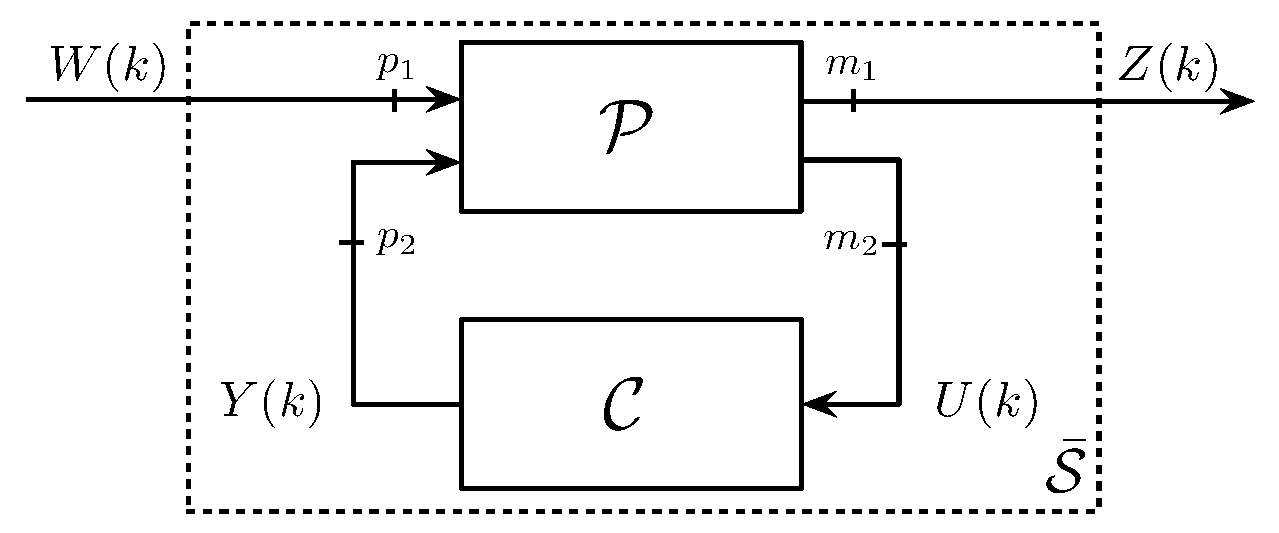
\includegraphics[width=0.6\textwidth]{standard_form.pdf}
		\caption{Closed-loop control system}
	\label{fig:standard_form}
\end{figure}

The controller is defined as $\mathcal{C}:=(Z,l,m_2,n,p_2)$ and the plant $\mathcal{P}$ as
\begin{equation}\label{eq:standard_form}
	\mathcal{P}:=
	\left(\begin{array}{c|cc}
		A & B_1 & B_2 \\
		\hline
		C_1 & D_{11} & D_{12} \\
		C_2 & D_{21} & 0		
	\end{array}\right)
\end{equation}
where $A\in\Rbb{\np}{\np}$, $B_1\in\Rbb{\np}{p_1}$, $B_2\in\Rbb{\np}{p_2}$, $C_1\in\Rbb{m_1}{\np}$, $C_2\in\Rbb{m_2}{\np}$, $D_{11}\in\Rbb{m_1}{p_1}$, $D_{12}\in\Rbb{m_1}{p_2}$, $D_{21}\in\Rbb{m_2}{p_1}$ and 	 $D_{22}\in\Rbb{m_2}{p_2}$ is assumed to be zero only to simplify the mathematical expressions.


The closed-loop system $\bar{\mathcal{S}}$ is then given by
\begin{equation}
	\bar{\mathcal{S}}=F_l(\mathcal{P},\mathcal{C}):=
	\left(\begin{array}{c|cc}
		\bar{A} & \bar{B} \\
		\hline\\[-3mm]
		\bar{C} & \bar{D}
	\end{array}\right)	
\end{equation}
%\cite[p. 8]{Alaz99a}
where  $F_l(\cdot,\cdot)$ is the well-known lower linear fractional transform \cite{Zhou96} and where $\bar{A}\in\Rbb{\np+n}{\np+n}$, $\bar{B}\in\Rbb{\np+n}{p_1}$, $\bar{C}\in\Rbb{m_1}{\np+n}$ and $\bar{D}\in\Rbb{m_1}{p_1}$ are such that
\begin{align}
		\bar{A}&= \begin{pmatrix}
			A + B_2 D_Z C_2	&\quad	B_2 C_Z \\
			B_Z C_2	&\quad	A_Z
		\end{pmatrix}, \label{eq:defAbar} &
		\bar{B} &= \begin{pmatrix}
			B_1 + B_2 D_Z D_{21} \\
			B_Z  D_{21}
		\end{pmatrix},\\
		\bar{C} &= \begin{pmatrix}
			C_1 + D_{12} D_Z C_2	&\quad	D_{12} C_Z
		\end{pmatrix}, &
		\bar{D} &=  D_{11} + D_{12} D_Z D_{21}.
\end{align}
The closed-loop transfer function is
\begin{equation}
%	\bar{H} : z \to \bar{C}\pa{zI_{\np+n}-\bar{A}}^{-1}\bar{B}+\bar{D}
% ?? slightly neater and dimension of I is obvious ??
	\bar{H} : z \mapsto \bar{C}\pa{zI -\bar{A}}^{-1}\bar{B}+\bar{D}.
\end{equation}


These notations will be used  in the toolbox.\\
Then, the following measures are considered:
\begin{itemize}
	\item the input-output sensitivity (\funcName[@FWR/MsensHcl]{MsensH\_cl})
		\begin{equation}
		 	\bar{M}_{L_{2}}^W = \norm{\dd{\bar{H}}{Z} \times r_{Z}}_2^2.
		 \end{equation}	
	\item the pole-sensitivity and related stability measure (\funcName[@FWR/MsensPolecl]{MsensPole\_cl} and \funcName[@FWR/Mstability]{Mstability})
	 	\begin{equation}
	 		\bar{\Psi} = \sum_{k=1}^n \norm{ \dd{\abs{\bar{\lambda}_k}}{Z} \times r_Z }_F^2.
	 	\end{equation}
	\item the roundoff noise gain (\funcName[@FWR/RNGcl]{RNG\_cl})
	
\end{itemize}

See \cite{Hila08b}.


%========================
% The optimal realization problem
%========================
\section{The optimal realization problem}


The problem of determining the best realization can be posed as follows:
\begin{problem}[Optimal realization problem]
	Consider a trans\-fer function $H$ and a sensitivity measure $\mathcal{J}$.
	The \I{optimal design problem} is to find the best realization $\mathcal{R}_{opt}$ with transfer function $H$ according to the criteria $\mathcal{J}$, that is
	\begin{equation}
		\mathcal{R}_{opt} = \underset{\mathcal{R}\in\mathscr{R}_H}{\arg\ \min\ } \mathcal{J}(\mathcal{R}).
	\end{equation}
\end{problem}

Due to the size of $\mathscr{R}_H$, this problem cannot be solved practically. Indeed, a solution may even have infinite dimension. Hence the following problem is introduced to restrict the search to a particular structuration.

\begin{problem}[Optimal structured realization problem]\label{pb:structured_design}
	The problem to find the optimal structured realization $\mathcal{R}_{opt}^{\mathscr{S}}$, that is
	\begin{equation}
		\mathcal{R}_{opt}^{\mathscr{S}} = \underset{\mathcal{R}\in\mathscr{R}_H^{\mathscr{S}}}{\arg\ \min\ } \mathcal{J}(\mathcal{R}).
	\end{equation}
\end{problem}%



The \I{Inclusion Principle} (Proposition \ref{prop:inclusion_principle2}) provides the means to search over the structured realizations set $\mathscr{R}_H^{\mathscr{S}}$.\\
Since the measure $\mathcal{J}$ could be non-smooth and/or non-convex, the Adaptive Simulated Annealing (ASA) \cite{Ingb96} method could be used  to solve  Problem \ref{pb:structured_design}. This method has worked well for other optimal realization problems \cite{Wu01}. \\
The FWR Toolbox can also use simplex or Quasi-Newton algorithm to solve problem \ref{pb:structured_design}.


%=======
% Tutorial
%=======
\section{Tutorial}


\subsection{First example}
Let's consider this discrete state-space system:
\begin{verbatim}
>> A = [ 1.4590 -0.91037 0.39565; 1 0 0; 0 0.5 0 ];
>> B = [ 0.5; 0; 0 ];
>> C = [ 0.28261 0.13244 0.15183 ];
>> D = 0.0031689;
>> Sys = ss(A,B,C,D, 1e-2);
\end{verbatim}
Then, we can create a first Finite Wordlength Realization
\begin{verbatim}
R = SS2FWR(Sys);
\end{verbatim}
First, let's display this FWR object
\begin{verbatim}
>> R
R has 1 input, 1 output, 3 states, and 0 intermediate variable.
Z=
   1.4590e+00  -9.1037e-01   3.9565e-01   5.0000e-01
   1.0000e+00            0            0            0
            0   5.0000e-01            0            0
   2.8261e-01   1.3244e-01   1.5183e-01   3.1689e-03
\end{verbatim}
It is also possible to display, for example, the associated matrices $Wo$ (observability grammian), $P$ and $W_Z$:
\begin{verbatim}
>> R.Wo
ans =
   1.0232e+00  -6.1354e-01   3.9081e-01
  -6.1354e-01   5.5557e-01  -2.7112e-01
   3.9081e-01  -2.7112e-01   1.8322e-01

>> R.P
ans =
   1.4590e+00  -9.1037e-01   3.9565e-01
   1.0000e+00            0            0
            0   5.0000e-01            0

>> R.WZ
ans =
     1     1     1     1
     0     0     0     0
     0     1     0     0
     1     1     1     1
\end{verbatim}
This last result shows that some coefficients will be considered as exactly implemented (coefficients where $(W_Z)_{ij}$ is null), whereas some will be modified during the quantization.\\
It is possible to ask for the input-output sensitivity and the sensitivity matrix
\begin{verbatim}
>> [M MZ] = MsensH(R)
M =
   1.4391e+01

MZ =
   1.9730e+00   1.9730e+00   9.8651e-01   1.0115e+00
            0            0            0            0
            0   8.4062e-01            0            0
   1.1358e+00   1.1358e+00   5.6788e-01   1.0000e+00
\end{verbatim}
To have the sensitivity for all the coefficients, it is possible to set $W_Z$ to 1
\begin{verbatim}
>> R.WZ=ones(4);
>> [M MZ] = MsensH(R);
>> MZ
MZ =
   1.9730e+00   1.9730e+00   9.8651e-01   1.0115e+00
   1.3716e+00   1.3716e+00   6.8582e-01   7.4536e-01
   8.4062e-01   8.4062e-01   4.2031e-01   4.2805e-01
   1.1358e+00   1.1358e+00   5.6788e-01   1.0000e+00
\end{verbatim}

Now, it could be interesting to find, among the equivalent state-space realizations, one that minimize this input-output sensitivity. For this purpose, we need to create a Finite Wordlength Structuration:
\begin{verbatim}
>> S = SS2FWS( Sys)
 has 1 input, 1 output, 3 states, and 0 intermediate variable.
Z=
   1.4590e+00  -9.1037e-01   3.9565e-01   5.0000e-01
   1.0000e+00            0            0            0
            0   5.0000e-01            0            0
   2.8261e-01   1.3244e-01   1.5183e-01   3.1689e-03
T=
     1     0     0
     0     1     0
     0     0     1
\end{verbatim}
In addition to a FWR object, a FWStructuration includes a parameter \matlab{T}, that allows to get all the state-space equivalent realizations $(T^{-1}AT,T^{-1}B,CT,D)$.\\
To consider a new realization, deduced from the original one with this transformation, we simply give a new value for $T$:
\begin{verbatim}
>> S.T=rand(3)
 has 1 input, 1 output, 3 states, and 0 intermediate variable.
Z=
   3.7455e-01   1.3029e+00  -4.6071e+00  -2.0013e+00
   2.1170e-01  -9.4236e-01   5.5850e+00   5.0983e-01
  -1.2475e-02  -4.9193e-01   2.0268e+00   1.8077e+00
   3.2995e-01   1.8533e-01   3.9119e-01   3.1689e-03
T=
   3.8156e-01   1.8687e-01   6.4631e-01
   7.6552e-01   4.8976e-01   7.0936e-01
   7.9520e-01   4.4559e-01   7.5469e-01
\end{verbatim}
The original realization is stored in \matlab{S.Rini}, whereas the actual realization is obtained with \matlab{S.R}.\\
It is important to remark that all the equivalent realizations deduced from the original one have the same $W_Z$ matrix. So, in order to consider fully parameterized realizations, it is important to set $W_Z$ to a matrix with all coefficients set to 1, with \matlab{S.Rini.WZ=ones(size(S.Rini.WZ));}.\\
It is possible to compare these two realizations and their I/O-sensitivity


\begin{verbatim}
>> MsensH(S.Rini)
ans =
   1.4391e+01

>> MsensH(S.R)
ans =
   5.8668e+02
\end{verbatim}

Now, the most interesting thing is to search for the optimal realization.\\
First, we need to set the options for the search
\begin{verbatim}
>> options = {'method','simplex','Display','Iter','MaxFunEvals',1e4};
\end{verbatim}
Then, we can run the optimization:
\begin{verbatim}
>> S = optim( S, optins, @MsensH)
\end{verbatim}

The options are cells of pairs. Some options concern the \funcName[@FWS/optim]{optim} methods, while some are directly passed to the Matlab optimization algorithm used (\matlab{fminsearch}, \matlab{fminunc}, ...).
\matlab{\{'method','simplex'\}} allows to use the \matlab{fminsearch} algorithm, whereas \matlab{\{'Display','Iter'\}} and \matlab{\{'MaxFunEvals',1e4\}} allow to display each iteration and set the maximum number of function evaluation to $10^4$. See \matlab{optimset} for all the possible options and the method \funcName[@FWS/optim]{optim} for all the possible options.

\matlab{S} has now the \I{optimal} value for $T$.






%===========
% The classes
%===========
\section{The classes}
The the \matlab{FWR toolbox} is based on two classes:
\begin{itemize}
	\item the \matlab{FWR} class to describe the Finite Wordlength Realizations
	\item the \matlab{FWS} class for the Finite Wordlength Structurations
\end{itemize}


%==========================
\subsection{The \matlab{FWR} class}

The \matlab{FWR} class describes a realization expressed with the SIF (see def. \ref{def:realization}). It contains the following fields:
\begin{itemize}
	\item \matlab{l}, \matlab{m}, \matlab{n} and \matlab{p} : dimensions of the realization ($l$ intermediate variables, $m$ inputs, $n$ states and $p$ outputs)
	\item \matlab{J}, \matlab{K}, \matlab{L}, \matlab{M}, \matlab{N}, \matlab{P}, \matlab{Q}, \matlab{R} and \matlab{S} : correspond to matrices $J$ to $S$
	\item \matlab{Z} : the $Z$ matrix defined in \eqref{eq:def_Z} from $J$ to $S$
	\item  \matlab{WJ}, \matlab{WK}, \matlab{WL}, \matlab{WM}, \matlab{WN}, \matlab{WP}, \matlab{WQ}, \matlab{WR} and \matlab{WS} : the weighting matrices $W_J$ to $W_S$  (they imply which parameter is exactly implemented ($0$, $\pm1$, a power of two or any number that will not be changed during the quantization), see \eqref{eq:defW})
	\item \matlab{WZ} : the $W_Z$ matrix
	\item \matlab{AZ}, \matlab{BZ}, \matlab{CZ} and \matlab{AZ} : matrices $A_Z$, $B_Z$, $C_Z$ and $D_Z$ (see equations \eqref{eq:defAZandBZ} and \eqref{eq:defCZandDZ})
	\item \matlab{Wc}, \matlab{Wo} : commandability and observability gramians $W_c$ and $W_o$
	\item \matlab{FPIS} : a \I{Fixed-Point Implementation Scheme} (see section \ref{sec:FPIS})
	\item \matlab{fp}, \matlab{block}, \matlab{rZ} : these fields are related to the coefficient representation
	\begin{itemize}
		\item \matlab{fp} : sets if the implementation uses the fixed-point or the floating-point representation. \matlab{fp} can take the values \matlab{'fixed'} (1=default) or \matlab{'floating'} (2).
		\item \matlab{block} : sets the coefficient's block. Coefficients in the same block share the same representation (binary-point position). \matlab{block} can take the values \matlab{'full'} (1), \matlab{'natural'} (2=default), or \matlab{'none'} (3).
		\item \matlab{rZ} : gives how much $Z$ is changed during the quantization process : $Z$ is perturbed to $Z+r_Z\times\Delta$ where
 	\begin{equation}
 		r_Z \triangleq
 		\begin{cases}
 			W_Z & \text{for fixed-point representation,} \\
 			2\eta_Z \times W_Z & \text{for floating-point representation,}
 		\end{cases}
 	\end{equation}
 	and $\eta_Z$ is such that
 	\begin{equation}
 		\pa{\eta_Z}_{i,j} \triangleq
 			\left\lbrace\begin{array}{l}
 				\text{the largest absolute value of}\\
 				\text{the block in which }  Z_{i,j} \text{ resides.}
 			\end{array}\right.
 	\end{equation}
	\end{itemize}
		These fields are only used for the sensitivities measure (\funcName[@FWR/MsensH]{MsensH}, \funcName[@FWR/MsensPole]{MsensPole}, ...), and are independent from the FPIS. These fields will probably disapear.\\
		See \cite{Hila07b} for \I{block-fixed-point} and \I{block-floating-point} representation.

\end{itemize}

When a FWR object is created, it is not possible to change its dimensions (fields \matlab{l}, \matlab{m}, \matlab{n} and \matlab{p} or the size of the matrices) or the fields \matlab{AZ}, \matlab{BZ}, \matlab{CZ}, \matlab{AZ}, \matlab{Wc} and \matlab{Wo}.\\
Fields \matlab{Z} and \matlab{WZ} are redundant with fields \matlab{J} to \matlab{S} and \matlab{WJ} to \matlab{WS}, but they can both be usefull. Changing \matlab{Z} automatically changes fields \matlab{J} to \matlab{S} and reciprocally (the same with \matlab{WZ}). Fields \matlab{AZ}, \matlab{BZ}, \matlab{CZ}, \matlab{AZ}, \matlab{Wc} and \matlab{Wo} are deduced accordingly.

%
\subsubsection{Fixed-Point Implementation Scheme}\label{sec:FPIS}

The FPIS is a structure to set the \I{Fixed-Point Implementation Scheme}. It is composed by:
 	\begin{itemize}
 		\item the fixed-point format of the input $(\beta_U,\gamma_U)$
 		and its maximum magnitude value $\overset{\max}{U}$
 		\item the fixed-point format of the intermediate variables $(\beta_T,\gamma_T)$
 		\item the fixed-point format of the states $(\beta_X,\gamma_X)$
 		\item the fixed-point format of the output $(\beta_Y,\gamma_Y)$
 		\item the fixed-point format of the coefficients $(\beta_Z,\gamma_Z)$
 		\item the fixed-point format of the accumulator $(\beta_{ADD}+\beta_{G},\gamma_{ADD})$ ($\beta_G$ guard bits)
 		\item the right-shift bits after each scalar product $d_{ADD}$ (\matlab{shiftADD})
 		\item the right-shift bits after each multiplication by a coefficient $d_Z$ (\matlab{shiftZ})
 		\item the computational scheme : \I{Roundoff After Multiplication} (RAM) or \I{Roundoff Before Multiplication} (RBM)
 	\end{itemize}

 	The algorithm
 	\begin{align*}
 		&\text{[i]} & JT(k+1) & \leftarrow MX(k) + NU(k)\\
 		&\text{[ii]} & X(k+1)  & \leftarrow KT(k+1) + PX(k) + QU(k)\\
 		&\text{[iii]} & Y(k)    & \leftarrow LT(k+1) + RX(k) + SU(k)
 	\end{align*}
 	requires to implement $l+n+p$ scalar products.\\
 	Each scalar product
 	\begin{equation}
 		S = \sum_{i=1}^n P_i E_i
 	\end{equation}
 	where $\pa{P_i}_{1 \leq i \leq n}$ are given coefficients and
 	$\pa{E_i}_{1 \leq i \leq n}$ some bounded variables, can be
 	implemented according to the following algorithms \ref{algo:setFPIS:RAM} and
 	\ref{algo:setFPIS:RBM}, and where $P'_i$, $E'_i$ and $S'_i$ are the integer representations
 	(according to their fixed-point format) to $P_i$,$E_i$ and
 	$S_i$.\\
	\begin{multicols}{2}{
 	\begin{algorithm}[H]
		\caption{\I{Roundoff After Multiplication} (RAM)\label{algo:setFPIS:RAM}}
 		$Add\leftarrow 0$\\
 		\For{$i$ from 0 to $n$}{$Add\leftarrow \pa{ P_i' * E_i' } >> d_i$}
 		$S'_i \leftarrow Add >> d'_i$
 	\end{algorithm} \ \\
 	\begin{algorithm}[H]
		\caption{\I{Roundoff Before Multiplication} (RBM)\label{algo:setFPIS:RBM}}
 		$Add\leftarrow 0$\\
 		\For{$i$ from 0 to $n$}{$Add\leftarrow \pa{ P_i' >> d_i } * E_i'$}
 		$S'_i \leftarrow Add >> d_i'$
 	\end{algorithm}}
	\end{multicols}
	Of course, $d_i$ represents the right-shift after each multiplication and $d'_i$ represents the final shift. They respectively correspond to the $d_Z$ and $d_{ADD}$ shift in the SIF algorithm.

 	The user may specify all the wordlengths ($\beta_U$, $\beta_T$, $\beta_X$, $\beta_Y$, $\beta_{ADD}$, $\beta_g$
 	and $\beta_Z$) and $\overset{\max}{U}$.
	
	See \cite{Hila08c} and the function \funcName[@FWR/setFPIS]{setFPIS} for more details.



%
\subsubsection{Methods}

The FWR's methods are : \\
% Generated by SimpleDoc (�T. Hilaire) - 09-Mar-2009

\begin{longtable}{|p{3.4cm}|p{8.4cm}|}
	\hline \funcName[complexFFT]{complexFFT} & Create FFT with complex coefficients (for FFT2FWR)\\
	\hline \funcName[strideM]{strideM} & Create a stride permutation matrix (for FFT2FWR)\\
	\hline \funcName[twiddleM]{twiddleM} & Create a diagonal matrix of twiddle factors (for FFT2FWR)\\
	\hline
\end{longtable}


%=========================
\subsection{The \matlab{FWS} class}\label{sec:FWSclass}

The \matlab{FWS} class describes a structuration and the way to search over the set of equivalent realizations of this structuration. This is done by defining the parameters used to search over the equivalent set and how theses parameters give new realizations (via the $\mt{U}\mt{Y}\mt{W}$-transformation, eq. \eqref{eq:UYWtransformation}, or directly).

%When creating a structuration, the goal is to help to manipulate equivalent realizations in that structuration (set of realizations with a given structure). For example, the equivalent state-space realizations can be handled with a structuration created by the command
%\begin{verbatim}
%	S = SS2FWS( ss(A,B,C,D,Te) );
%\end{verbatim}
%Then, it is possible to consider a realization, with state-space structure, from  a transformation matrix $T$


It contains the following fields :
\begin{itemize}
	\item \matlab{Rini} : the initial realization of this structuration (all the other equivalent structured realizations are computed \I{from} this realization),
	\item \matlab{R} : the actual considered realization,
	\item \matlab{paramsName} : name of the parameters used to search over the equivalent set,
	\item \matlab{paramsValue} : value of this parameters (they define the actual considered realization \matlab{R}),
	\item \matlab{paramsSize} : size of these parameters,
	\item \matlab{indices} : vector of indices. To do the optimization, the values of the parameters are put together in a row vector, and \matlab{indices} stores these indices, in that row, of each parameters (it is used when some parameters are fixed during the optimization). This is also internally used when some parameters are fixed,
	\item \matlab{UYWfun} : handle to a function that gives the transformation matrices $\mt{U}$, $\mt{Y}$ and $\mt{W}$ from the parameters,
	\item \matlab{Rfun} : handle to a function that gives the realization from the parameters (when the \matlab{UYWfun} cannot be defined),
	\item \matlab{dataMeasure} : cell of extra data used for the FWL measures (to store values that do not change from one realization to another equivalent) : every FWL measure can add what it needs inside,
	\item \matlab{dataFWS} : cell of extra data used to store internal values (can be used when defining a structuration).
\end{itemize}

The parameters (their names, values and sizes are stored in \matlab{paramsName}, \matlab{paramsValue} and \matlab{paramsSize}) can be used directly by their names, like any other fields : if \matlab{S} is a structuration, with parameters named \matlab{'T1'} and \matlab{'T2'}, expressions \matlab{S.T1} and \matlab{S.T2} allow to access the corresponding values.\\
All the fields of the \matlab{FWS} class are accessible with the \matlab{.fieldname} method (\matlab{get}), but it is only possible to change \matlab{Rini}  and the parameters (it is not possible to change their sizes). And changing one parameter will automatically change \matlab{R}.

When a structuration \matlab{S} is defined, it is then possible to search over all the equivalent realizations with the same structuration by changing the values of the associated parameters (those where the names are in \matlab{paramsName}). \matlab{S.R} gives the new realization (automatically update when \matlab{paramsValue} change, with \matlab{S.\I{paramName}=...}). This can be done with the \funcName[@FWS/optim]{optim} method, that uses quasi-Newton, simplex or ASA algorithm.

There is two ways to define how the parameters give a new realization. Only one of the two fields \matlab{UYWfun} and  \matlab{Rfun} must be filled. The function \matlab{UYWfun} must be preferred, because it allows to compute more quickly the FWL measures whose comportment with the $\mt{UYW}$-transformation is defined.

%
\subsubsection{\matlab{UYWfun} function}
	\desc{Purpose}
		The \matlab{UYWfun} is a function that defines how to search over all the equivalent realizations. It transforms the parameters of the structuration (given by \matlab{args}) in transformation matrices $\mt{U}$, $\mt{Y}$ and $\mt{W}$. The \matlab{cost\_flag} indicates if the transformation is valid.
	\desc{Syntax}
		\matlab{function [U,Y,W,cost\_flag] = \I{my\_UYW\_fun}( Rini, paramsValue, dataFWS)}
	\desc{Arguments}
		\begin{tabular}{l@{\ :\ }l}
			\matlab{U,Y,W} & matrices $\mt{U}$, $\mt{Y}$ and $\mt{W}$ \\
			\matlab{cost\_flag} & boolean that indicates if the parameters forms a valid transformation \\
			\matlab{Rini} & initial FW Realization \\
			\matlab{paramsValue} & cells of parameters values\\
			\matlab{dataFWS} & cell of extra data (that can be used to store internal values)
		\end{tabular}\\		

The parameters' values are accessible with \matlab{paramsValue} : the $i$\textsuperscript{th} parameter (in the order it is built) is given by \matlab{paramsValue\{i\}}. Most of the time, \matlab{Rini} and \matlab{dataFWS} are not useful (\matlab{U}, \matlab{Y} and \matlab{W} often directly depend on \matlab{paramsValue}).

%
\subsubsection{\matlab{Rfun} function}
	\desc{Purpose}
		The \matlab{Rfun} is a function that directly creates a new realization from the parameters' values, without returning $\mt{U}$, $\mt{Y}$ and $\mt{W}$ matrices.
	\desc{Syntax}
		\matlab{function [R,cost\_flag] = \I{my\_R\_fun}( Rini, paramsValue, dataFWS)}
	\desc{Arguments}
		\begin{tabular}{l@{\ :\ }l}
			\matlab{R} & new realization \\
			\matlab{cost\_flag} & boolean that indicates if the parameters forms a valid transformation \\
			\matlab{Rini} & initial FW Realization \\
			\matlab{paramsValue} & cells of parameters' values \\
			\matlab{dataFWS} & cell of extra data (that can be used to store internal values)
		\end{tabular}\\	

Everyone who creates a FWS should follow theses definitions.

%
\subsubsection{Methods}
The FWS's methods are : \\
% Generated by SimpleDoc (�T. Hilaire) - 09-Mar-2009

\begin{longtable}{|p{3.4cm}|p{8.4cm}|}
	\hline \funcName[complexFFT]{complexFFT} & Create FFT with complex coefficients (for FFT2FWR)\\
	\hline \funcName[strideM]{strideM} & Create a stride permutation matrix (for FFT2FWR)\\
	\hline \funcName[twiddleM]{twiddleM} & Create a diagonal matrix of twiddle factors (for FFT2FWR)\\
	\hline
\end{longtable}





%==========================
% FWR functions/methods reference
%==========================
\newpage
\section{FWR Toolbox reference}

% create
\subsection{create realizations and structurations}
In additions to the FWR/FWS's methods, the following functions can be used to create classical realizations and structurations : \\

% Generated by SimpleDoc (�T. Hilaire) - 09-Mar-2009

\begin{longtable}{|p{3.4cm}|p{8.4cm}|}
	\hline \funcName[complexFFT]{complexFFT} & Create FFT with complex coefficients (for FFT2FWR)\\
	\hline \funcName[strideM]{strideM} & Create a stride permutation matrix (for FFT2FWR)\\
	\hline \funcName[twiddleM]{twiddleM} & Create a diagonal matrix of twiddle factors (for FFT2FWR)\\
	\hline
\end{longtable}

Here is the detailed list:

% Generated by SimpleDoc (�T. Hilaire) - 09-Mar-2009

\begin{command}[@FWR/algorithmCfloat]{algorithmCfloat}
	\desc{Purpose}
Return the algorithm associated to this realization.
The algorithm is written in C-code with float
	\desc{Syntax}
\matlab{code = algorithmCfloat( R, funcName)}
	\desc{Parameters}
		\begin{tabular}{l@{\ :\ }p{9cm}}
\matlab{code} &  resulting C-code (with float)                  \\
\matlab{R} &  FWR object                                        \\
\matlab{funcName} &  name of the C-function (default=\matlab{myFilter})\\
		\end{tabular}
	\desc{Description}
Transform in \texttt{C}-code with \texttt{float} the algorithm of the realization:
\begin{align*}
&\text{[i]} & JT(k+1) & \leftarrow MX(k) + NU(k)\\
&\text{[ii]} & X(k+1)  & \leftarrow KT(k+1) + PX(k) + QU(k)\\
&\text{[iii]} & Y(k)    & \leftarrow LT(k+1) + RX(k) + SU(k)
\end{align*}
All the operations with matrices are expanded, and null multiplications are removed, identity multiplications are simplified, etc.\\
The input or a pointer to the vector of inputs is given to the function. The function returns the output or a pointer to a vector of putputs.\\
The intermediate variables are stored in a variable \matlab{T}. The states are stored in \matlab{static} variables \matlab{xn} and \matlab{xnp} (\matlab{xnp} is not necessary if $P$ is upper triangular), and a permutation of the vector (a permutation of the pointer to the vector) is performed for the next call.
	\desc{Example}
\begin{lstlisting}[language=C]
>> algorithmCfloat(R)
ans =
float myFilter( float u)
{
// states
static float* xn = (float*) calloc( 8*sizeof(float));
// intermediate variables
float T = -0.6630104844*xn[0] + 2.9240526562*xn[1] + -4.8512758825*xn[2]
+ 3.5897338871*xn[3] + 0.0000312390*xn[4] + 0.0001249559*xn[5]
+ 0.0001874339*xn[6] + 0.0001249559*xn[7] + 0.0000312390*u    ;
// output(s)
y = T    ;
// states
xn[0] = xn[1];
xn[1] = xn[2];
xn[2] = xn[3];
xn[3] = T    ;
xn[4] = xn[5];
xn[5] = xn[6];
xn[6] = xn[7];
xn[7] = u    ;
}
\end{lstlisting}
\desc{See also}
\funcName[@FWR/algorithmLaTeX]{algorithmLaTeX}
\end{command}



\begin{command}[@FWR/algorithmLaTeX]{algorithmLaTeX}
	\desc{Purpose}
Return the pseudocode algorithm described in \LaTeX
(to be used with package {algorithm2e})
	\desc{Syntax}
\matlab{code = algorithmLaTeX( R)         }\\
\matlab{code = algorithmLaTeX( R, caption)}
	\desc{Parameters}
		\begin{tabular}{l@{\ :\ }p{9cm}}
\matlab{R} &  FWR object                                  \\
\matlab{caption} &  caption used to describe the algorithm\\
\matlab{} &  (default=\matlab{'Pseudocode algorithm ...'})         \\
		\end{tabular}
	\desc{Description}
Return a \LaTeX-code that describe the algorithm of the realization:
\begin{align*}
&\text{[i]} & JT(k+1) & \leftarrow MX(k) + NU(k)\\
&\text{[ii]} & X(k+1)  & \leftarrow KT(k+1) + PX(k) + QU(k)\\
&\text{[iii]} & Y(k)    & \leftarrow LT(k+1) + RX(k) + SU(k)
\end{align*}
All the operations with matrices are expanded, and null multiplications are removed, identity multiplications are simplified, etc.\\
The package \textit{algorithm2e} is used.\\
The file \matlab{@FWR/private/myFilter.tex.template} is used as a
template.
	\desc{Example}
The following \LaTeX-code is produced by this function:
\begin{lstlisting}[language={[LaTeX]tex}]
\begin{algorithm}[h]
\caption{Pseudocode algorithm ...}
\KwIn{$u$: real}
\KwOut{$y$: real}
\KwData{$xn, xnp$: array [1..13] of reals}
\SetLine
\Begin{
\tcp{\emph{Intermediate variables}}
$xnp(1) \leftarrow 0.5529838718*xn(1) + -0.5379265439*xn(2) + 0.0291718129*xn(3) + 0.6715678041*u    $\;
$xnp(2) \leftarrow 0.5379265439*xn(1) + 0.0971133953*xn(2) + -0.3562792507*xn(3) + -0.3237597311*u    $\;
$xnp(3) \leftarrow 0.0291718129*xn(1) + 0.3562792507*xn(2) + -0.0728567423*xn(3) + 0.0792887747*u    $\;
\tcp{\emph{Outputs}}
$y      \leftarrow 0.6715678041*xn(1) + 0.3237597311*xn(2) + 0.0792887747*xn(3) + 0.0985311609*u    $\;
\tcp{\emph{Permutations}}
$xn \leftarrow xnp$\;
}
\end{algorithm}
\end{lstlisting}
And it corresponds to the algorithm \ref{algo:algorithmLaTeX:algo}:
\begin{algorithm}[h!]
\caption{Pseudocode algorithm ...\label{algo:algorithmLaTeX:algo}}
\KwIn{$u$: real}
\KwOut{$y$: real}
\KwData{$xn, xnp$: array [1..13] of reals}
\SetLine
\Begin{
\tcp{\emph{Intermediate variables}}
$xnp(1) \leftarrow 0.5529838718*xn(1) + -0.5379265439*xn(2) + 0.0291718129*xn(3) + 0.6715678041*u    $\;
$xnp(2) \leftarrow 0.5379265439*xn(1) + 0.0971133953*xn(2) + -0.3562792507*xn(3) + -0.3237597311*u    $\;
$xnp(3) \leftarrow 0.0291718129*xn(1) + 0.3562792507*xn(2) + -0.0728567423*xn(3) + 0.0792887747*u    $\;
\tcp{\emph{Outputs}}
$y      \leftarrow 0.6715678041*xn(1) + 0.3237597311*xn(2) + 0.0792887747*xn(3) + 0.0985311609*u    $\;
\tcp{\emph{Permutations}}
$xn \leftarrow xnp$\;
}
\end{algorithm}
\desc{See also}
\funcName[@FWR/algorithmCfloat]{algorithmCfloat}, \funcName[@FWR/implementLaTeX]{implementLaTeX}
\end{command}



\begin{command}[@FWR/computationalCost]{computationalCost}
	\desc{Purpose}
Give the number of additions and multiplications implied in the realization
	\desc{Syntax}
\matlab{[add, mul] = computationalCost( R, tol)}
	\desc{Parameters}
		\begin{tabular}{l@{\ :\ }p{9cm}}
\matlab{add} &  number of additions             \\
\matlab{mul} &  number of multiplications       \\
\matlab{R} &  FWR object                        \\
\matlab{tol} &  tolerance (default value = 1e-8)\\
		\end{tabular}
	\desc{Description}
The number of additions and multiplications is based on the number of trivial parameters
and null parameters.\\
The evaluation is based on the following proposition, applied on the three steps [i],
[ii] and [iii] of algorithm \eqref{eq:def_implicit} :
\begin{proposition}
Let $Y\in\Rbb{a}{b}$ be a constant, and $V\in\Rbb{b}{1}$ a variable.\\
The calculus $YV$ needs $a(b-1)-n^0_Y$ additions and $ab-n^1_Y$ multiplications, where
$n^0_Y$ is the number of null elements of $Y$ and $n^1_Y$ is the number of trivial elements
($0$,$1$,$-1$) of $Y$ (these elements don't imply a multiplication)
\end{proposition}
Then, the algorithm requires $(l+n+p)(l+m+n-1)-l-n^0_Z$ additions and $(l+n+p)(l+m+n)-n^1_Z$
multiplications.
\end{command}



\begin{command}[@FWR/computeW]{computeW}
	\desc{Purpose}
Compute (or update) the weighting matrices ($W_J$ to $W_S$, and $W_Z$) of a FWR object
	\desc{Syntax}
\matlab{R = computeW(R,tol)}
	\desc{Parameters}
		\begin{tabular}{l@{\ :\ }p{9cm}}
\matlab{R} &  FWR object                                                  \\
\matlab{tol} &  tolerance (default=1e-8) (maximal distance to 0, -1 or +1)\\
		\end{tabular}
	\desc{Description}
For $X$ in $\{J,K,L,M,N,P,Q,R,S\}$ and $X=Z$, the weighting matrices
$W_J$, $W_K$, $W_L$, $W_M$, $W_N$, $W_P$, $W_Q$, $W_R$, $W_S$ and $W_Z$ are computed according to
\begin{equation}
(W_X)_{ij} = \left\{
\begin{array}{ll}
0 & \text{if } \abs{X_{ij}}<\epsilon \text{ or } \abs{X_{ij}+1}<\epsilon \text{ or } \abs{X_{ij}-1}<\epsilon \\
1 & \text{else}
\end{array}\right.
\end{equation}
Where $\epsilon$ is the tolerance ($1e-8$ as default value). Here,
the proximity to $0$ and $\pm1$ are considered (the other power of 2 are not considered).
\end{command}



\begin{command}[@FWR/display]{display}
	\desc{Purpose}
Display the realization (dimensions and Z)
	\desc{Syntax}
\matlab{display(R)}
	\desc{Parameters}
		\begin{tabular}{l@{\ :\ }p{9cm}}
\matlab{R} &  FWR object\\
		\end{tabular}
	\desc{Description}
Display the dimensions (inputs, outputs, states and intermediate variables) and $Z$.
	\desc{Example}
\begin{verbatim}
R has 1 input, 1 output, 4 states, and 0 intermediate variable.
3.5897e+00  -1.2128e+00   3.6551e-01  -1.6575e-01   1.5625e-02
4.0000e+00            0            0            0            0
0		2.0000e+00            0            0            0
0            0   5.0000e-01            0            0
1.5174e-02   5.7416e-04   1.7304e-03   1.6844e-04   3.1239e-05
\end{verbatim}
\desc{See also}
\funcName[@FWS/display]{display}
\end{command}



\begin{command}[@FWR/double]{double}
	\desc{Purpose}
Convert FWR object to double (return Z matrix)
	\desc{Syntax}
\matlab{d = double(R)}
	\desc{Parameters}
		\begin{tabular}{l@{\ :\ }p{9cm}}
\matlab{d} &  double    \\
\matlab{R} &  FWR object\\
		\end{tabular}
	\desc{Description}
return the $Z$ matrix.
\desc{See also}
\funcName[@FWR/display]{display}
\end{command}



\begin{command}[@FWR/FWR]{FWR}
	\desc{Purpose}
FWR class' constructor
	\desc{Syntax}
\matlab{R = FWR()                            }\\
\matlab{R = FWR(R1)                          }\\
\matlab{R = FWR(J,K,L,M,N,P,Q,R,S, fp, block)}
	\desc{Parameters}
		\begin{tabular}{l@{\ :\ }p{9cm}}
\matlab{R} &  FWR object created                                                                                                                                     \\
\matlab{R1} &  FWR object to be copied                                                                                                                               \\
\matlab{J,K,...,S} &  matrices of the realization                                                                                                                    \\
\matlab{fp} &  fixed-point or floating-point representation                                                                                                          \\
\matlab{} & \matlab{'fixed'} (default value) or \matlab{'floating'}                                                                                                                    \\
\matlab{block} &  block-representation scheme. The coefficients in a same block share the same representation (same scale factor, etc...). Take the following values:\\
\matlab{} &  \matlab{'full'}: same representation for all coefficients of R                                                                                                   \\
\matlab{} &  \matlab{'natural'} (default value): blocks are made of matrices J,K,L,M,N,P,Q,R,S                                                                                \\
\matlab{} &  \matlab{'none'}: each coefficient has its own representation (according to its value)                                                                            \\
		\end{tabular}
	\desc{Description}
Constructor of the \matlab{FWR} class.\\
It could create an empty object ($l=m=n=p=0$), copy an object or create a \matlab{FWR} object from matrices $J$ to $S$: in that case, the other parameters are deduced (only $0$, $1$ or $-1$ are considered as exactly implemented).
\desc{See also}
\funcName[@FWS/FWS]{FWS}
\end{command}



\input{SimpleDoc/@FWR/FWRmat2LaTeX.tex}
\begin{command}[@FWR/get]{get}
	\desc{Purpose}
Get some properties of a FWR object
(or list the properties if \matlab{propName} is ignored)
	\desc{Syntax}
\matlab{value = get(R, propName)}
	\desc{Parameters}
		\begin{tabular}{l@{\ :\ }p{9cm}}
\matlab{value} &  value of the property            \\
\matlab{R} &  FWR object                           \\
\matlab{propName } &  name of the property (string)\\
		\end{tabular}
	\desc{Description}
This function is most of the time called by \funcName{@FWR/subsref}.\\
The value of every field (\matlab{l}, \matlab{m}, \matlab{n} and \matlab{p} ; \matlab{J},
\matlab{K}, \matlab{L}, \matlab{M}, \matlab{N}, \matlab{P}, \matlab{Q}, \matlab{R} and \matlab{S};
\matlab{Z} ; \matlab{WJ}, \matlab{WK}, \matlab{WL}, \matlab{WM}, \matlab{WN}, \matlab{WP},
\matlab{WQ}, \matlab{WR} and \matlab{WS} ;	\matlab{WZ} ; \matlab{AZ}, \matlab{BZ}, \matlab{CZ}
and \matlab{AZ}) can be evaluated with this command, but \matlab{l}, \matlab{m}, \matlab{n}, \matlab{p},
\matlab{AZ}, \matlab{BZ}, \matlab{CZ} and \matlab{AZ} cannot be modified.\\
Changing \matlab{Z} changes fields \matlab{J} to \matlab{S}, and reciprocally (this is
the same with \matlab{WZ}).
\desc{See also}
\funcName[@FWR/set]{set}, \funcName[@FWR/subsref]{subsref}, \funcName[@FWR/subsasgn]{subsasgn}, \funcName[@FWS/get]{get}
\end{command}



\begin{command}[@FWR/implementLaTeX]{implementLaTeX}
	\desc{Purpose}
Return the associated fixed-point algorithm described in \LaTeX
(to be used with package \matlab{algorithm2e})
	\desc{Syntax}
\matlab{code = implementLaTeX( R)         }\\
\matlab{code = implementLaTeX( R, caption)}
	\desc{Parameters}
		\begin{tabular}{l@{\ :\ }p{9cm}}
\matlab{R} &  FWR object                                      \\
\matlab{caption} &  caption used to describe the algorithm    \\
\matlab{} &  (default = \matlab{'Numerical fixed-point algorithm ...'})\\
		\end{tabular}
	\desc{Description}
Return the associated fixed-point algorithm in \LaTeX. It uses the package
\textit{algorithm2e}. All the wordlengths and the fixed-point positions should be
first computed by adjusting the FPIS with
\funcName{@FWR/setFPIS}.\\
The file \matlab{@FWR/private/myFilter.tex.template} is used as a
template.
	\desc{Example}
It returns \LaTeX-code like this
\begin{lstlisting}[language={[LaTeX]tex}]
\begin{algorithm}[h]
\caption{Numerical fixed-point algorithm ...}
\KwIn{$u$: 16 bits integer}
\KwOut{$y$: 16 bits integer}
\KwData{$xn, xnp$: array [1..13] of 16 bits integers}
\KwData{$Acc$: 32 bits integer}
\SetLine
\Begin{
\tcp{\emph{Intermediate variables}}
$Acc \leftarrow (xn(1) * 18120)$\;
$Acc \leftarrow Acc + (xn(2) * -8813)$\;
$Acc \leftarrow Acc + (xn(3) * 239)$\;
$Acc \leftarrow Acc + (u     * 11003)$\;
$xnp(1) \leftarrow Acc >> 15$\;
$Acc \leftarrow (xn(1) * 17627)$\;
$Acc \leftarrow Acc + (xn(2) * 1591)$\;
$Acc \leftarrow Acc + (xn(3) * -2919)$\;
$Acc \leftarrow Acc + (u     * -5304)$\;
$xnp(2) \leftarrow Acc >> 14$\;
$Acc \leftarrow (xn(1) * 3824)$\;
$Acc \leftarrow Acc + (xn(2) * 23349)$\;
$Acc \leftarrow Acc + (xn(3) * -2387)$\;
$Acc \leftarrow Acc + (u     * 5196)$\;
$xnp(3) \leftarrow Acc >> 15$\;
\tcp{\emph{Outputs}}
$Acc \leftarrow (xn(1) * 22006)$\;
$Acc \leftarrow Acc + (xn(2) * 5304)$\;
$Acc \leftarrow Acc + (xn(3) * 650)$\;
$Acc \leftarrow Acc + (u     * 1614)$\;
$y      \leftarrow Acc >> 14$\;
\tcp{\emph{Permutations}}
$xn \leftarrow xnp$\;
}
\end{algorithm}
\end{lstlisting}
That corresponds to the algorithm \ref{algo:implementLaTeX:algo}.
\begin{algorithm}[h]
\caption{Numerical fixed-point algorithm ...\label{algo:implementLaTeX:algo}}
\KwIn{$u$: 16 bits integer}
\KwOut{$y$: 16 bits integer}
\KwData{$xn, xnp$: array [1..13] of 16 bits integers}
\KwData{$Acc$: 32 bits integer}
\SetLine
\Begin{
\tcp{\emph{Intermediate variables}}
$Acc \leftarrow (xn(1) * 18120)$\;
$Acc \leftarrow Acc + (xn(2) * -8813)$\;
$Acc \leftarrow Acc + (xn(3) * 239)$\;
$Acc \leftarrow Acc + (u     * 11003)$\;
$xnp(1) \leftarrow Acc >> 15$\;
$Acc \leftarrow (xn(1) * 17627)$\;
$Acc \leftarrow Acc + (xn(2) * 1591)$\;
$Acc \leftarrow Acc + (xn(3) * -2919)$\;
$Acc \leftarrow Acc + (u     * -5304)$\;
$xnp(2) \leftarrow Acc >> 14$\;
$Acc \leftarrow (xn(1) * 3824)$\;
$Acc \leftarrow Acc + (xn(2) * 23349)$\;
$Acc \leftarrow Acc + (xn(3) * -2387)$\;
$Acc \leftarrow Acc + (u     * 5196)$\;
$xnp(3) \leftarrow Acc >> 15$\;
\tcp{\emph{Outputs}}
$Acc \leftarrow (xn(1) * 22006)$\;
$Acc \leftarrow Acc + (xn(2) * 5304)$\;
$Acc \leftarrow Acc + (xn(3) * 650)$\;
$Acc \leftarrow Acc + (u     * 1614)$\;
$y      \leftarrow Acc >> 14$\;
\tcp{\emph{Permutations}}
$xn \leftarrow xnp$\;
}
\end{algorithm}
\desc{See also}
\funcName[@FWR/algorithmLaTeX]{algorithmLaTeX}, \funcName[@FWR/implementMATLAB]{implementMATLAB}, \funcName[@FWR/implementVHDL]{implementVHDL}
\end{command}



\begin{command}[@FWR/implementMATLAB]{implementMATLAB}
	\desc{Purpose}
Create the associated fixed-point algorithm in Matlab language
(it uses integer to simulate fixed-point). The algorithm is written in a file (by default, in \matlab{'myFilter.m'} file)
	\desc{Syntax}
\matlab{implementMATLAB( R,fileName)}
	\desc{Parameters}
		\begin{tabular}{l@{\ :\ }p{9cm}}
\matlab{R} &  FWR object                                                  \\
\matlab{fileName} &  filename of the created function (default=\matlab{'myFilter'})\\
		\end{tabular}
	\desc{Description}
Generate a Matlab file (named \matlab{'myFilter.m'} by default) that emulates the fixed-point algorithm
corresponding to the realization. The rounding operations are realized by the \texttt{floor} function.
All the wordlengths and the fixed-point positions should be first computed by adjusting the FPIS with
\funcName{@FWR/setFPIS}.\\
The file \matlab{@FWR/private/myFilter.m.template} is used as a
template.
	\desc{Example}
It creates a matlab file like
\begin{lstlisting}%[language=matlab]
% Fixed-point algorithm in Matlab language
% (it uses integer to simulate fixed-point)
%
% y = myFilter(u)
%
% y: filtered output(s)
% u: intput(s)
%
% date: 08-Dec-2008 18:12:26
% Automatically generated by implementMATLAB / FWRToolbox
function y = myFilter(u)
% initialize
u = round(2.^11.*u);
y = zeros( size(u,1), 1 );
xn = zeros(3,1);
xnp = zeros(3,1);
for i=1:size(u,1)
% intermediate variables
Acc0 = xn(1) * 18120;
Acc0 = Acc0 + xn(2) * -8813;
Acc0 = Acc0 + xn(3) * 239;
Acc0 = Acc0 + u(i)  * 11003;
xnp(1) = floor( Acc0/2^15 );
Acc1 = xn(1) * 17627;
Acc1 = Acc1 + xn(2) * 1591;
Acc1 = Acc1 + xn(3) * -2919;
Acc1 = Acc1 + u(i)  * -5304;
xnp(2) = floor( Acc1/2^14 );
Acc2 = xn(1) * 3824;
Acc2 = Acc2 + xn(2) * 23349;
Acc2 = Acc2 + xn(3) * -2387;
Acc2 = Acc2 + u(i)  * 5196;
xnp(3) = floor( Acc2/2^15 );
% output(s)
Acc3 = xn(1) * 22006;
Acc3 = Acc3 + xn(2) * 5304;
Acc3 = Acc3 + xn(3) * 650;
Acc3 = Acc3 + u(i)  * 1614;
y(i)   = floor( Acc3/2^14 );
%permutations
xn = xnp;
end
y = 2.^-11.*y;
\end{lstlisting}
It could be used to compute the fixed-point output of the associated realization, with the fixed-point
algorithm.
\begin{verbatim}
>> u=10*rand(1000,1);
>> y=myFilter(u);
\end{verbatim}
\desc{See also}
\funcName[@FWR/implementLaTeX]{implementLaTeX}, \funcName[@FWR/implementVHDL]{implementVHDL}
\end{command}



\begin{command}[@FWR/implementVHDL]{implementVHDL}
	\desc{Purpose}
Create the associated fixed-point algorithm in VHDL.
Two files are generated \matlab{'xxxx\_entity.vhd'} and \matlab{'xxx\_types.vhd'} where
xxxx is the name given (\matlab{'myFilter'} by default)
	\desc{Syntax}
\matlab{implementVHDL( R,fileName)}
	\desc{Parameters}
		\begin{tabular}{l@{\ :\ }p{9cm}}
\matlab{R} &  FWR object                                      \\
\matlab{fileName} &  name of the function (default=\matlab{myFilter})\\
		\end{tabular}
	\desc{Description}
Generate two VHDL files (named "myFilter\_entity.vhd" and "myFilter\_types.vhd" by default)
that realizes the fixed-point algorithm corresponding to the
realization.\\
All the wordlengths and the fixed-point positions should be first computed by adjusting the FPIS with
\funcName{@FWR/setFPIS}.\\
The files \matlab{@FWR/private/FP\_types.vhd.template} and \matlab{@FWR/private/FP\_entity.vhd.template} are used as a
template.
	\desc{Example}
This function produces a \texttt{myFilter\_types.vhdl} file
\begin{lstlisting}[language=VHDL]
library IEEE;
use IEEE.STD_LOGIC_1164.all;
use IEEE.STD_LOGIC_arith.all;
use IEEE.STD_LOGIC_SIGNED.all;
-- purpose: filtering (generic fixed-point specificatin)
-- type   : sequential/arithmetic
-- inputs : u(n)
-- output : y(n)
-- author : automatically generated by
-- date   : 08-Dec-2008 18:41:00
package FP_types is
-- input data with FP format (16,4,11)
subtype datain is integer range -2**15 to 2**15-1;
-- filtered output data with FP format (16,4,11)
subtype dataout is integer range -2**15 to 2**15-1;
-- states
subtype state1 is integer range -2**15 to 2**15-1;   -- format (16,5,10)
subtype state2 is integer range -2**15 to 2**15-1;   -- format (16,4,11)
subtype state3 is integer range -2**15 to 2**15-1;   -- format (16,3,12)
-- intermediate variables
end FP_types;
\end{lstlisting}
It also produces a \texttt{myFilter\_entity.vhdl} file
\begin{lstlisting}[language=VHDL]
library IEEE;
use IEEE.STD_LOGIC_1164.all;
use IEEE.STD_LOGIC_arith.all;
use IEEE.STD_LOGIC_SIGNED.all;
library work;
use work.FP_types.all;
entity myFilter is
port (
rstb    : in  std_logic; -- asynchronous reset asynchrone active low
clk     : in  std_logic; -- global clock
u       : in  datain; -- input data
y       : out dataout); -- filtered output
end myFilter;
architecture RTL of myFilter is
-- states
signal xn1 : state1 := 0;
signal xn2 : state2 := 0;
signal xn3 : state3 := 0;
-- intermediate variables
begin
-- output(s)
y <= (    xn1 * 22006 + xn2 * 5304 + xn3 * 650 + u   * 1614) / 2**14;
S1: process(rstb,clk)
begin
if rstb = '0' then                  -- asynchronous reset
xn1 <= 0;
xn2 <= 0;
xn3 <= 0;
elsif clk'event and clk = '1' then  -- rising clock edge
-- states
xn1 <= (    xn1 * 18120 + xn2 * (-8813) + xn3 * 239 + u   * 11003) / 2**15;
xn2 <= (    xn1 * 17627 + xn2 * 1591 + xn3 * (-2919) + u   * (-5304)) / 2**14;
xn3 <= (    xn1 * 3824 + xn2 * 23349 + xn3 * (-2387) + u   * 5196) / 2**15;
end if;
end process S1;
end RTL;
\end{lstlisting}
\desc{See also}
\funcName[@FWR/implementLaTeX]{implementLaTeX}, \funcName[@FWR/implementMATLAB]{implementMATLAB}
\end{command}



\begin{command}[@FWR/l2scaling]{l2scaling}
	\desc{Purpose}
Perform a $L_2$-scaling on the FWR
	\desc{Syntax}
\matlab{R = l2scaling(R, Wcii)}\\
\matlab{[U,Y,W] = l2scaling(R)}
	\desc{Parameters}
		\begin{tabular}{l@{\ :\ }p{9cm}}
\matlab{R} &  FWR object                                                                 \\
\matlab{U,Y,W } &  transformation matrices applied on R                                  \\
\matlab{Wcii } &  vector (size $(1,l+n)$) of controllability gramians desired            \\
\matlab{} &  if \matlab{Wcii} is omitted, strict $L_2$-scaling is applied ( \matlab{Wcii=ones(1,n+l)} )\\
		\end{tabular}
	\desc{Description}
Perform a $L_2$-scaling.\\
The scaling forces the transfer functions from the inputs to the states and the intermediate variables to have a unitary $L_2$-norm. Theses norms are given by the diagonal terms of $W_c$ and $J^{-1}\pa{NN^\top+MW_cM^\top}J^{-\top}$.\\
The $L_2$-scaling is a $\mt{U}\mt{Y}\mt{W}$-transformation where $\mt{U}$ and $\mt{W}$ are diagonal with:
\begin{eqnarray}
\pa{\mt{U}}_{ii} &=& \sqrt{\pa{W_c}_{ii}} \\
\pa{\mt{W}}_{ii} &=& \sqrt{\pa{J^{-1}\pa{NN^\top+MW_cM^\top}J^{-\top}}_{ii}}
\end{eqnarray}
It is also possible to assign some particular values for the diagonal terms of the two gramians.
\desc{See also}
\funcName[@FWR/relaxedl2scaling]{relaxedl2scaling}
	\desc{References}
\cite{Feng09a} Y.�Feng, P.�Chevrel, and T.�Hilaire. A practival strategy of an efficient and sparse FWL implementation of LTI filters. In submitted to ECC'09, 2009.\\
%\cite{Hila09a}	T.�Hilaire. Low parametric sensitivity realizations with relaxed l2-dynamic-range-scaling constraints. submitted to IEEE Trans. on Circuits \& Systems II, 2009.
\end{command}



\begin{command}[@FWR/MsensH]{MsensH}
	\desc{Purpose}
Compute the open-loop transfer function sensitivity measure (and the
sensitivity matrix)
	\desc{Syntax}
\matlab{[M MZ]  = MsensH(R)}
	\desc{Parameters}
		\begin{tabular}{l@{\ :\ }p{9cm}}
\matlab{M} &  sensitivity measure\\
\matlab{MZ} &  sensitivity matrix\\
\matlab{R} &  FWR object         \\
		\end{tabular}
	\desc{Description}
The open-loop transfer function sensitivity measure is defined by
\begin{equation}
M_{L_{2}}^W = \norm{\dede{H}{Z} \times r_{Z}}_{F}^2.
\end{equation}
where $\dede{H}{Z}\in\Rbb{l+n+p}{l+n+q}$ is the \I{transfer function sensitivity matrix}.
It is the matrix of the $L_{2}$-norm of the sensitivity of the transfer function $H$ with
respect to each coefficient  $Z_{i,j}$. It is defined by
\begin{equation}
\pa{\dede{H}{Z}}_{i,j} \triangleq \norm{\dd{H}{Z_{i,j}}}_{2},
\end{equation}
In SISO case, the $M_{L_{2}}^W$ measure is equal to
\begin{equation}
M_{L_{2}}^W = \norm{\dd{H}{Z} \times r_{Z}}_2^2
\end{equation}
and is then an extension to the SIF of the classical state-space sensitivity measure
\begin{equation}
M_{L_2} \triangleq \norm{\dd{H}{A}}_2^2 + \norm{\dd{H}{B}}_2^2 + \norm{\dd{H}{C}}_2^2.
\end{equation}
The $M_{L_2}^W$ measure can be evaluated by the following propositions
\begin{proposition}
\begin{equation}
\dd{H}{Z} =  H_1 \cd H_2
\end{equation}
where $H_1$ and $H_2$ are defined by
\begin{eqnarray}
H_1 : z &\mapsto& C_Z (zI_n-A_Z)^{-1} M_1 + M_2 \\
H_2 : z &\mapsto& N_2 + N_1 (zI_n-A_Z)^{-1} B_Z
\end{eqnarray}
with
\begin{align}
M_1 &\triangleq  \begin{pmatrix} KJ^{-1} & I_n & 0 \end{pmatrix}, &
M_2 &\triangleq  \begin{pmatrix} LJ^{-1} & 0 & I_{p_2} \end{pmatrix}, \\
N_1 &\triangleq  \begin{pmatrix} J^{-1}M \\ I_n \\ 0 \end{pmatrix}, &
N_2 &\triangleq  \begin{pmatrix} J^{-1}N \\ 0 \\ I_{m_2} \end{pmatrix}.
\end{align}
\end{proposition}
\begin{proposition}
The transfer function sensitivity matrix $\dede{H}{Z}$ can be computed as
\begin{equation}
\pa{ \dede{H}{Z} }_{i,j} = \norm{ H_1 E_{i,j} H_2 }_2
\end{equation}
with
\begin{equation}
H_1 E_{i,j} H_2 :=
\left(\begin{array}{cc|c}
A_Z & 0 & B_Z \\
M_1 E_{i,j} N_1 & A & M_1 E_{i,j} N_2 \\
\hline \vspace{-3.5mm}\\
M_2 E_{i,j} N_1 & C_Z & M_2 E_{i,j} N_2
\end{array}\right)
\end{equation}
and $E_{i,j}$ is the matrix of appropriate size with all elements being $0$ except the $(i,j)$th element which is unity.
\end{proposition}
\begin{remark}
In the SISO case, the problem becomes simpler by noting that
\begin{align}
\pa{ \dede{H}{Z} }_{i,j} &=  \norm{ (H_2H_1)_{i,j} }_2 \\
&= \norm{
\left(\begin{array}{cc|c}
A_Z & 0 & B_Z \\
M_1 N_1 & A_Z & M_1 N_2 \\
\hline \vspace{-3.5mm}\\
M_2 N_1 & C_Z & M_2 N_2
\end{array}\right)_{i,j}}_2
\end{align}
The $(l+n+1)\times(l+n+1)$ $H_2$-norm evaluations here require  only $l+n+1$ Lyapunov equations to be solved .
\end{remark}
\desc{See also}
\funcName[@FWR/MsensHcl]{MsensH\_cl}, \funcName[@FWR/wprodnorm]{w\_prod\_norm}
	\desc{References}
\cite{Hila07d}	T.�Hilaire and P.�Chevrel. On the compact
formulation of thederivation of a transfer matrix with respect to
another matrix. Technical Report RR-6760, INRIA, 2008.\\
\cite{Hila06a} T.�Hilaire, P.�Chevrel, and J.-P. Clauzel. Low
parametric sensitivity realization design for FWL implementation
of MIMO controllers : Theory and application to the active control of vehicle longitudinal oscillations. In Proc. of Control Applications of Optimisation CAO'O6, April 2006.\\
\cite{Hila07b} T.�Hilaire, P.�Chevrel, and J.�Whidborne. A
unifying framework for finite wordlength realizations. IEEE Trans.
on Circuits and Systems, 8(54), August 2007.\\
\end{command}



\begin{command}[@FWR/MsensHcl]{MsensH\_cl}
	\desc{Purpose}
Compute the closed-loop transfer function sensitivity measure (and the
sensitivity matrix)
	\desc{Syntax}
\matlab{[M MZ]  = MsensH\_cl( R, Sysp)}
	\desc{Parameters}
		\begin{tabular}{l@{\ :\ }p{9cm}}
\matlab{M} &  sensitivity measure        \\
\matlab{MZ} &  sensitivity matrix        \\
\matlab{R} &  FWR object                 \\
\matlab{Sysp} &  plant system (ss object)\\
		\end{tabular}
	\desc{Description}
The closed-loop transfer function sensitivity measure is very similar to the open-loop transfer function sensitivity. It is defined by
\begin{equation}
\bar{M}_{L_{2}}^W = \norm{\dede{\bar{H}}{Z} \times r_{Z}}_{F}^2.
\end{equation}
where $\dede{\bar{H}}{Z}\in\Rbb{l+n+p}{l+n+q}$ is the \I{transfer function sensitivity matrix}.
It is the matrix of the $L_{2}$-norm of the sensitivity of the transfer function $\bar{H}$ with
respect to each coefficient  $Z_{i,j}$. It is defined by
\begin{equation}
\pa{\dede{\bar{H}}{Z}}_{i,j} \triangleq \norm{\dd{\bar{H}}{Z_{i,j}}}_{2},
\end{equation}
In SISO case, the $\bar{M}_{L_{2}}^W$ measure is equal to
\begin{equation}
\bar{M}_{L_{2}}^W = \norm{\dd{\bar{H}}{Z} \times r_{Z}}_2^2.
\end{equation}
The $M_{L_2}^W$ measure can be evaluated by the following
propositions\cite{Hila07d}
\begin{proposition}
\begin{equation}
\dd{\bar{H}}{Z} =  \bar{H}_1 \cd \bar{H}_2
\end{equation}
where $H_1$ and $H_2$ are defined by
\begin{eqnarray}
\bar{H}_1 : z &\mapsto& \bar{C}\pa{ zI-\bar{A} }^{-1} \bar{M}_1 + \bar{M}_2 \\
\bar{H}_2 : z &\mapsto& \bar{N}_1 \pa{ zI-\bar{A} }^{-1}\bar{B} + \bar{N}_2
\end{eqnarray}
with
\begin{eqnarray}
\bar{M}_1 = \begin{pmatrix}
B_2LJ^{-1} & 0 & B_2 \\
KJ^{-1} & I_n & 0
\end{pmatrix} &&
\bar{N}_1 =\begin{pmatrix}
J^{-1}NC_2 & J^{-1}M \\
0 & I_{n} \\
C_2 & 0
\end{pmatrix}\\
\bar{M}_2 = \begin{pmatrix} D_{12}LJ^{-1} & 0 & D_{12} \end{pmatrix} &&
\bar{N}_2 = \begin{pmatrix} J^{-1}ND_{21} \\ 0 \\ D_{21} \end{pmatrix}
\end{eqnarray}
\end{proposition}
\desc{See also}
\funcName[@FWR/MsensH]{MsensH}, \funcName[@FWR/wprodnorm]{w\_prod\_norm}
	\desc{References}
\cite{Hila07d}	T.�Hilaire and P.�Chevrel. On the compact
formulation of the derivation of a transfer matrix with respect to
another matrix. Technical Report RR-6760, INRIA, 2008.\\
\cite{Hila07e}	T.�Hilaire, P.�Chevrel, and J.�Whidborne. Low
parametric closed-loop sensitivity realizations using fixed-point
and floating-point arithmetic. In Proc. European Control Conference (ECC'07), July 2007.\\
\cite{Hila08b}	T.�Hilaire, P.�Chevrel, and J.�Whidborne. Finite
wordlength controller realizations using the specialized implicit
form. Technical Report RR-6759, INRIA, 2008.\\
\end{command}



\begin{command}[@FWR/MsensPole]{MsensPole}
	\desc{Purpose}
Compute the open-loop pole sensitivity measure
(and the pole sensitivity matrix) for a FWR object
	\desc{Syntax}
\matlab{[M, dlambda\_dZ, dlk\_dZ] = MsensPole( R, moduli)}
	\desc{Parameters}
		\begin{tabular}{l@{\ :\ }p{9cm}}
\matlab{M} &  pole sensitivity measure                                                                                    \\
\matlab{dlambda\_dZ} &  the pole sensitivity matrix                                                                        \\
\matlab{dlk\_dZ} &  pole sensitivity matrices for each pole                                                                \\
\matlab{R} &  FWR object                                                                                                  \\
\matlab{moduli } &  1 (default value) : compute $\dd{\abs{\lambda}}{Z}$ (the sensitivity of the moduli of the eigenvalues)\\
\matlab{} &  0 : compute $\dd{\lambda}{Z}$ (without the moduli)                                                           \\
		\end{tabular}
	\desc{Description}
The pole sensitivity measure of $\mathcal{R}$ is defined by
\begin{equation}
\Psi = \sum_{k=1}^n \norm{ \dd{\abs{\lambda_k}}{Z} \times r_Z }_F^2.
\end{equation}
(it is also possible to only consider the sensitivity of $\lambda_k$ instead of the sensitivity of $\abs{\lambda_k}$.
This measure can be evaluated with
\begin{equation}
\dd{\abs{\lambda_k}}{Z} =
\begin{pmatrix}	KJ^{-1} & I & 0 	\end{pmatrix}^\top
\dd{\abs{\lambda_k}}{A}
\begin{pmatrix} J^{-1}M \\ I \\ 0 \end{pmatrix}^\top
\end{equation}
and the following lemma\cite{Wu01}:
\begin{lemma}\label{prop:MsensPole:dlambda}
Let $M\in\Rbb{n}{n}$ be diagonalizable. Let $\pa{\lambda_{k}}_{1 \leq k \leq n}$ be its eigenvalues, and $\pa{x_{k}}_{1 \leq k \leq n}$ the corresponding right eigenvectors. Denote $M_{x} \triangleq \begin{pmatrix}x_{1} x_{2} \hdots x_{n}\end{pmatrix}$ and $M_{y} = \begin{pmatrix}y_{1} y_{2} \hdots y_{n}\end{pmatrix} \triangleq M_{x}^{-H}$. Then
\begin{equation}\label{eq:MsensPole:dlambda}
\dd{\lambda_{k}}{M} = y_{k}^\ast x_{k}^\top \hspace{3mm} \forall k=1,\hdots,n
\end{equation}
and
\begin{equation}\label{eq:MsensPole:dmodulilambda}
\dd{\abs{\lambda_{k}}}{M} = \frac{1}{\abs{\lambda_{k}}}Re\pa{\lambda_{k}^\ast \dd{\lambda_{k}}{M}}
\end{equation}
where $\cdot^\ast$ denotes the conjugate operation, $Re(\cdot)$ the real part and $\cdot^H$ the transpose conjugate operator.
\end{lemma}
A \I{pole sensitivity matrix} can also be constructed to evaluate the overall impact of each coefficient. Let  $\dede{\abs{\lambda}}{Z}$ denote the pole sensitivity matrix defined by
\begin{equation}
\pa{\dede{\abs{\lambda}}{Z}}_{i,j} \triangleq \sqrt{ \sum_{k=1}^n \pa{\dd{\abs{\lambda_k}}{Z_{i,j}}}^2}.
\end{equation}%
Then, The pole sensitivity measure is then given by:
\begin{equation}
\Psi=\norm{\dede{\abs{\lambda}}{Z} \times r_Z}_F^2.
\end{equation}
\desc{See also}
\funcName[@FWR/MsensPolecl]{MsensPole\_cl}, \funcName[@FWR/Mstability]{Mstability}, \funcName[@FWR/deigdZ]{deigdZ}, \funcName[@FWS/MsensPole]{MsensPole}
	\desc{References}
\cite{Hila06b}	T.�Hilaire, P.�Chevrel, and J.-P. Clauzel. Pole
sensitivity stability related measure of FWL realization with the
implicit state-space formalism. In 5th IFAC Symposium on Robust Control Design (ROCOND'06), July 2006.\\
\cite{Hila07b}	T.�Hilaire, P.�Chevrel, and J.�Whidborne. A unifying framework for finite wordlength realizations. IEEE Trans. on Circuits and Systems, 8(54), August 2007.
\end{command}



\begin{command}[@FWS/MsensPolecl]{MsensPole\_cl}
	\desc{Purpose}
Compute the closed-loop pole sensitivity measure for a FWS object.
The computation is based on the UYW-transform
	\desc{Syntax}
\matlab{M = MsensPole\_cl( S, U,Y,W, Sysp,moduli)}
	\desc{Parameters}
		\begin{tabular}{l@{\ :\ }p{9cm}}
\matlab{M} &  pole sensitivity measure                                                                                        \\
\matlab{S} &  FWS object                                                                                                      \\
\matlab{U,Y,W } &  transformation matrices                                                                                    \\
\matlab{Sysp} &  plant system (ss object)                                                                                     \\
\matlab{moduli } &  1 (default value) : compute $\dd{\abs{\bar\lambda}}{Z}$ (the sensitivity of the moduli of the eigenvalues)\\
\matlab{} &  0 : compute $\dd{\bar\lambda}{Z}$ (without the moduli)                                                           \\
		\end{tabular}
	\desc{Description}
This function computes the closed-loop pole sensitivity measure for a FWS object. It is based on the $\mt{U}\mt{Y}\mt{W}$-transform.\\
If we consider $\mt{T}_1$ and $\mt{T}_2$ such that
\begin{equation}
Z_1 = \mt{T}_1	Z_0 \mt{T}_2
\end{equation}
\begin{equation}
\mt{T}_1 = \begin{pmatrix}
\mt{Y}\\
&\mt{U}^{-1}\\
&&I_{p}
\end{pmatrix}, \hspace{5mm}
\mt{T}_2 = \begin{pmatrix}
\mt{W}\\
&\mt{U}\\
&&I_{m}
\end{pmatrix}
\end{equation}
then the sensitivity measure for $Z_1$ can be computed from the sensitivity for $Z_0$ with
\begin{equation}
\en{ \dd{\abs{\bar\lambda_k}}{Z} }_{Z_1} =  \mt{T}_1^{-\top} \en{ \dd{\abs{\bar\lambda_k}}{Z} }_{Z_0} \mt{T}_2^{-\top}
\end{equation}
These matrix $\en{ \dd{\abs{\bar\lambda_k}}{Z} }_{Z_0}$ are stored in the \matlab{dataMeasure} field.
\desc{See also}
\funcName[@FWS/MsensPole]{MsensPole}, \funcName[@FWR/MsensPolecl]{MsensPole\_cl}
	\desc{References}
\cite{Hila08b} T.�Hilaire, P.�Chevrel, and J.�Whidborne. Finite wordlength controller realizations using the specialized implicit form. Technical Report RR-6759, INRIA, 2008.
\end{command}



\begin{command}[@FWS/Mstability]{Mstability}
	\desc{Purpose}
Compute the closed-loop pole sensitivity stability related measure for a FWS object.
The computation is based on the UYW-transform
	\desc{Syntax}
\matlab{M = Mstability( S, U,Y,W, Sysp, moduli)}
	\desc{Parameters}
		\begin{tabular}{l@{\ :\ }p{9cm}}
\matlab{M} &  pole sensitivity measure                                                                                        \\
\matlab{S} &  FWS object                                                                                                      \\
\matlab{U,Y,W } &  transformation matrices                                                                                    \\
\matlab{Sysp} &  plant system (ss object)                                                                                     \\
\matlab{moduli } &  1 (default value) : compute $\dd{\abs{\bar\lambda}}{Z}$ (the sensitivity of the moduli of the eigenvalues)\\
\matlab{} &  0 : compute $\dd{\bar\lambda}{Z}$ (without the moduli)                                                           \\
		\end{tabular}
	\desc{Description}
This function computes the closed-loop pole sensitivity stability
related measure for a FWS object. It is based on the
UYW-transform.\\
If we consider $\mt{T}_1$ and $\mt{T}_2$ such that
\begin{equation}
Z_1 = \mt{T}_1	Z_0 \mt{T}_2
\end{equation}
\begin{equation}
\mt{T}_1 = \begin{pmatrix}
\mt{Y}\\
&\mt{U}^{-1}\\
&&I_{p}
\end{pmatrix}, \hspace{5mm}
\mt{T}_2 = \begin{pmatrix}
\mt{W}\\
&\mt{U}\\
&&I_{m}
\end{pmatrix}
\end{equation}
then the sensitivity measure for $Z_1$ can be computed from the sensitivity for $Z_0$ with
\begin{equation}
\en{ \dd{\abs{\bar\lambda_k}}{Z} }_{Z_1} =  \mt{T}_1^{-\top} \en{ \dd{\abs{\bar\lambda_k}}{Z} }_{Z_0} \mt{T}_2^{-\top}
\end{equation}
These matrix $\en{ \dd{\abs{\bar\lambda_k}}{Z} }_{Z_0}$ are stored in the \matlab{dataMeasure} field.
\desc{See also}
\funcName[@FWR/Mstability]{Mstability}, \funcName[@FWS/MsensPolecl]{MsensPole\_cl}
	\desc{References}
\cite{Hila08b} T.�Hilaire, P.�Chevrel, and J.�Whidborne. Finite wordlength controller realizations using the specialized implicit form. Technical Report RR-6759, INRIA, 2008.
\end{command}



\begin{command}[@FWR/mtimes]{mtimes}
	\desc{Purpose}
Multiply two FWR (put them in cascade)
	\desc{Syntax}
\matlab{R = R1*R2        }\\
\matlab{R = mtimes(R1,R2)}
	\desc{Parameters}
		\begin{tabular}{l@{\ :\ }p{9cm}}
\matlab{R} &  FWR result           \\
\matlab{R1} &  first operand (FWR) \\
\matlab{R2} &  second operand (FWR)\\
		\end{tabular}
	\desc{Description}
\fig[scale=0.3]{cascade}{Two realizations in cascade}
Put two realization in cascade (see figure \ref{fig:cascade}).\\
We consider two realizations $\mathcal{R}_1:=(J_1,K_1,L_1,M_1,N_1,P_1,Q_1,R_1,S_1)$
and $\mathcal{R}_2:=(J_2,K_2,L_2,M_2,N_2,P_2,Q_2,R_2,S_2)$ (with compatible size,
\I{i.e.} $p_1=m_2$).\\
By introducing an intermediate variable $T$ equal to the output of $\mathcal{R}_1$,
the resulting realization $\mathcal{R}$ can be expressed in the implicit form by :
\begin{footnotesize}
\begin{equation*}
\begin{pmat}({..|.|})
J_1 & 0 & 0 & 0 & 0 & 0 \cr
-L_1 & I & 0 & 0 &0 & 0 \cr
0 & -N_2 & J_2 & 0 & 0 & 0 \cr\-
-K_1 & 0 & 0 & I & 0 & 0 \cr
0 & -Q_2 & -K_2 & 0 & I & 0 \cr\-
0 & -S_2 & -L_2 & 0 & 0 & I \cr
\end{pmat}
\begin{pmatrix}
T_1(k+1) \\
T(k+1) \\
T_2(k+1) \\
X_1(k+1) \\
X_2(k+1) \\
Y_2(k)
\end{pmatrix}
=
\begin{pmat}({..|.|})
0 & 0 & 0 & M_1 & 0 & N_1 \cr
0 & 0 & 0 & R_1 & 0 & S_1 \cr
0 & 0 & 0 & 0 & M_2 & 0 \cr\-
0 & 0 & 0 & P_1 & 0 & Q_1 \cr
0 & 0 & 0 & 0 & P_2 & 0 \cr\-
0 & 0 & 0 & 0 & R_2 & 0 \cr
\end{pmat}
\begin{pmatrix}
T_1(k) \\
T(k) \\
T_2(k) \\
X_1(k) \\
X_2(k) \\
U_1(k)
\end{pmatrix}
\end{equation*}
\end{footnotesize}
\desc{See also}
\funcName[@FWR/plus]{plus}
\end{command}



\begin{command}[@FWR/ONP]{ONP}
	\desc{Purpose}
Compute the Output Noise Power for a FWR object with Roundoff Before
Multiplication (RBM) computational scheme
	\desc{Syntax}
\matlab{M = ONP( R, roundingMode)}
	\desc{Parameters}
		\begin{tabular}{l@{\ :\ }p{9cm}}
\matlab{M} &  output noise power measure                                           \\
\matlab{R} &  FWR object                                                           \\
\matlab{mode} &  indicates the truncation mode: \matlab{'truncation'} (default) or \matlab{'nearest'}\\
		\end{tabular}
	\desc{Description}
This function computes the Output Noise Power.\\
Let us consider a realization $\mathcal{R}$ described with the implicit form�\eqref{eq:def_implicit}, with transfer function $H$.
When implemented, the steps (i) to (iii) are modified by the add of noises $\xi_T(k)$, $\xi_X(k)$ and $\xi_Y(k)$:
\begin{equation}\label{eq:ONP:implemented_sys}
\begin{array}{r>{\hspace{-3mm}}c<{\hspace{-3mm}}l}
J.T(k+1)  &\leftarrow&  M.X(k) + N.U(k) + \xi_T(k) \\
X(k+1)  &\leftarrow&  K.T(k+1) + P.X(k) + Q.U(k) + \xi_X(k) \\
Y(k)  &\leftarrow&  L.T(k+1) + R.X(k) + S.U(k) + \xi_Y(k)
\end{array}
\end{equation}
%(the noise $J^{-1}\xi_T(k)$ is added on $T(k+1)$).\\
These noises added depend on:
\begin{itemize}
\item the way the computations are organized (the order of the sums) and done,
\item the fixed-point representation of the inputs, the outputs,
\item and the fixed-point representation chosen for the states, the intermediate variables and the coefficients.
\end{itemize}
%They are determined by their first ($\mu$) and second ($\Psi$, $\sigma$) order moments.
They are modeled as independent white noise, characterized by their first and second order moments.
Denote $\xi$ the vector with all the added noise sources:
\begin{equation}
\xi(k) \triangleq \begin{pmatrix} \xi_T(k) \\ \xi_X(k) \\ \xi_Y(k) \end{pmatrix}
\end{equation}
\begin{proposition}
It is then possible to express the implemented system as the initial system with a noise $\xi'(k)$ added on the output(s) (see figure \ref{fig:equivalent_system}).
\fig[scale=0.4]{equivalent_system}{Equivalent system, with noises extracted}\\
$\xi'(k)$ is the noise $\xi(k)$ through the transfer function $H_\xi$ defined by:
\begin{equation}
H_\xi : z \to C_Z \pa{ zI_{n}-A_Z}^{-1} M_1 + M_2
\end{equation}
with
\begin{eqnarray}
M_1 &\triangleq  \begin{pmatrix} KJ^{-1} & I_n & 0 \end{pmatrix} \\
M_2 &\triangleq  \begin{pmatrix} LJ^{-1} & 0 & I_{p_2} \end{pmatrix}
\end{eqnarray}
\end{proposition}
The Output Noise Power is defined as the power of the noises added on the output
\begin{equation}
P \triangleq E{ \xi'(k)\xi'(k)^\top }
\end{equation}
where the $E{.}$ is the mean operator.\\
It is evaluated by \cite{Hila08c}:
\begin{equation}\label{eq:RNP}
P = tr\pa{ \psi_\xi \pa{ M_2^\top M_2 + M_1^\top W_o M_1 } } +  \mu_{\xi'}^\top \mu_{\xi'}
\end{equation}
where $\mu_{\xi'} = (C_Z(I-A_Z)^{-1}M_1+M_2)\mu_\xi$ and $W_o$ is the observability gramian of the system $\mathcal{R}$.
Then, in \I{Roundoff Before Multiplication} (RBM) scheme, the quantizations only occur at the end of the additions, when the accumulator result is stored in intermediate variables, states or output, and a right-shift of $d_{ADD}$ bits is applied.
The lemma \ref{prop:quantization_noise} recalls the noise produced during shift:
\begin{lemma}\label{prop:quantization_noise}
Let $x(k)$ be a signal with fixed-point format $(\beta+d,\alpha+d)$. Right shifting $x(k)$ of $d$ bits is similar to add to $x(k)$ the independent white noise $e(k)$.\\% (see figure \ref{fig:quantization_noise}).
%	\fig[scale=0.4]{quantization_noise}{Quantized a signal is similar to add a noise}\\
The right shift could round $x(k)$ towards $-\infty$ (truncation: default behaviour) or toward the nearest integer (nearest rounding: possible with some additional hardware/software operations \cite{Laps96}). If $d>0$, the moments of $e(k)$ are given by:
\begin{equation}
\begin{array}{|c|c|c|}
\hline & \text{truncation} & \text{best roundoff}\\
\hline \mu_e & 2^{-\gamma-1}(1-2^{-d}) & 2^{-\gamma-d-1} \\
\hline \sigma_e^2 & \frac{2^{-2\gamma}}{12}(1-2^{-2d}) & \frac{2^{-2\gamma}}{12}(1-2^{-2d}) \\
\hline
\end{array}
\end{equation}
else ($d\leq0$) $e(k)$ is null.
\end{lemma}
It is now possible to define the moments of $\xi(k)$:
Denote $\bar{\gamma} \triangleq \begin{pmatrix} \gamma_T \\ \gamma_X \\ \gamma_Y \end{pmatrix}$ and define $s$ by
\begin{equation}
s_i \triangleq \begin{cases}
1 & \text{if } d_{ADDi} > 0 \\
0 & \text{otherwise}
\end{cases}
\end{equation}
Then $\mu_\xi$ is given by:
\begin{equation}
\pa{\mu_\xi}_{i} = \begin{cases}
s_i 2^{-\bar{\gamma}_i-1}  & \text{truncation}\\
s_i 2^{-\bar{\gamma}_i-1-d_{ADD}} & \text{nearest rounding}
\end{cases}
\end{equation}
and, since these noises are independent, $\psi_\xi$ is diagonal with:
\begin{equation}
\pa{\psi_\xi}_{i,i} = s_i\frac{2^{-2\bar{\gamma}_i}}{12} \pa{ 1 - 2^{-d_{ADD}}  }
\end{equation}
\desc{See also}
\funcName[@FWR/setFPIS]{setFPIS}, \funcName[@FWR/RNG]{RNG}
	\desc{References}
\cite{Hila08c} T.�Hilaire, D.�M�nard, and O.�Sentieys. Bit
accurate roundoff noise analysis of fixed-point linear controllers. In Proc. IEEE International Symposium on Computer-Aided Control System Design (CACSD'08), September 2008.
\end{command}



\begin{command}[@FWR/plus]{plus}
	\desc{Purpose}
add two FWR object (put them in parallel)
	\desc{Syntax}
\matlab{R = R1+R2                  }\\
\matlab{R = plus(R1,R2,generalform)}
	\desc{Parameters}
		\begin{tabular}{l@{\ :\ }p{9cm}}
\matlab{R} &  FWR result                                                                \\
\matlab{R1} &  first FWR                                                                \\
\matlab{R2} &  second FWR                                                               \\
\matlab{generalform} &  (default is true) to use the general form (or a particular form)\\
		\end{tabular}
	\desc{Description}
\fig[scale=0.3]{parallel}{Two realizations in parallel}
Put two realization in parallel (see figure \ref{fig:parallel}).\\
We consider two realizations $\mathcal{R}_1:=(J_1,K_1,L_1,M_1,N_1,P_1,Q_1,R_1,S_1)$
and $\mathcal{R}_2:=(J_2,K_2,L_2,M_2,N_2,P_2,Q_2,R_2,S_2)$ (with compatible size, \I{i.e.}
$m_1=m_2$ and $p_1=p_2$).\\
By introducing the intermediate variables $T_1'$ and $T_2'$ equal to the output
of the two realizations, the resulting realization $\mathcal{R}$ (\I{general} form)
can be expressed in the implicit form by
\begin{footnotesize}
\begin{equation*}
\begin{pmat}({...|.|})
J_1 & 0 & 0 &0 & 0 & 0 & 0 \cr
-L_1 & I_{p_1} & 0 & 0 & 0 &0 & 0 \cr
0 & 0 & J_2 & 0 & 0 &0 & 0 \cr
0 & 0 & -L_2 & I_{p_2} & 0 & 0 & 0 \cr\-
-K_1 & 0 & 0 & 0 & I_{n_1} & 0 & 0 \cr
0 & 0 & -K_2 & 0 & 0 & I_{n_2} & 0 \cr\-
0 & -I_{p} & 0 & -I_{p} & 0 & 0 & I_{p} \cr
\end{pmat}
\begin{pmatrix}
T_1(k+1) \\
T_1'(k+1) \\
T_2(k+1) \\
T_2'(k+1) \\
X_1(k+1) \\
X_2(k+1) \\
Y_2(k)
\end{pmatrix}
=
\begin{pmat}({...|.|})
0 & 0 & 0 & 0 & M_1 & 0 & N_1 \cr
0 & 0 & 0 & 0 & R_1 & 0 & S_1 \cr
0 & 0 & 0 & 0 & 0 & M_2 & N_2 \cr
0 & 0 & 0 & 0 & 0 & R_2 & S_2 \cr\-
0 & 0 & 0 & 0 & P_1 & 0 & Q_1 \cr
0 & 0 & 0 & 0 & 0 & P_2 & Q_2 \cr\-
0 & 0 & 0 & 0 & 0 & 0 & 0 \cr
\end{pmat}
\begin{pmatrix}
T_1(k) \\
T_1'(k) \\
T_2(k) \\
T_2'(k) \\
X_1(k) \\
X_2(k) \\
U_1(k)
\end{pmatrix}
\end{equation*}
\end{footnotesize}
If we allow to regroup $S_1$ and $S_2$ in one term $S$ (and changing a bit
the parametrization if $S_1$ and $S_2$ are both non-zero), the resulting
realization can be expressed in a \I{compact} form :
\begin{footnotesize}
\begin{equation*}
\begin{pmat}({.|.|})
J_1 & 0  & 0 & 0 & 0 \cr
0 &  J_2  & 0 &0 & 0 \cr\-
-K_1 & 0 & I_{n_1} & 0 & 0 \cr
0 & -K_2 & 0 & I_{n_2} & 0 \cr\-
-L_1 & -L_2 & 0 & 0 & I_{p} \cr
\end{pmat}
\begin{pmatrix}
T_1(k+1) \\
T_2(k+1) \\
X_1(k+1) \\
X_2(k+1) \\
Y_2(k)
\end{pmatrix}
=
\begin{pmat}({.|.|})
0 & 0 & M_1 & 0 & N_1 \cr
0 & 0 & 0 & M_2 & N_2 \cr\-
0 & 0 & P_1 & 0 & Q_1 \cr
0 & 0 & 0 & P_2 & Q_2 \cr\-
0 & 0 & R_1 & R_2 & \pa{S_1+S_2} \cr
\end{pmat}
\begin{pmatrix}
T_1(k) \\
T_1'(k) \\
T_2(k) \\
T_2'(k) \\
X_1(k) \\
X_2(k) \\
U_1(k)
\end{pmatrix}
\end{equation*}
\end{footnotesize}
If $S_1$ and/or $S_2$ are null, the two forms are equivalent (in finite precision).
\desc{See also}
\funcName[@FWR/mtimes]{mtimes}
\end{command}



\begin{command}[@FWR/quantized]{quantized}
	\desc{Purpose}
Return the quantized realization, according to a fixed-point implementation scheme
	\desc{Syntax}
\matlab{[Rqt, DeltaZ] = quantized( R);}
	\desc{Parameters}
		\begin{tabular}{l@{\ :\ }p{9cm}}
\matlab{Rqt} &  quantized realization (FWR object)                \\
\matlab{DeltaZ} &  approximation on $Z$ (it is NOT $Z-Z^\dagger$ )\\
\matlab{R} &  FWR object                                          \\
		\end{tabular}
	\desc{Description}
According to a fixed-point implementation scheme, this function returns the realization with quantized coefficients.
The binary point position of the coefficient depends on the computational scheme (\I{Roundoff Before Multiplication} or \I{Roundoff After Multiplication})
and is given by:
\begin{equation}
\tilde\gamma_Z = \begin{cases}
\gamma_Z & \text{if \I{RAM}}\\
\gamma_{ADD}.\VecOne{1}{l+n+m} - \VecOne{l+n+p}{1}. \begin{pmatrix} \gamma_T \\ \gamma_X \\ \gamma_U \end{pmatrix}^{\hspace{-2mm}\top} & \text{if \I{RBM}}
\end{cases}
\end{equation}
($\gamma_{ADD}$ is the binary point position of the adders, see
\cite{Hila08c} and \funcName[@FWR/setFPIS]{setFPIS}).\\
The new coefficients $Z^\dagger$ are then given by
\begin{equation}
Z^\dagger \triangleq 2^{-\gamma_Z} \left\lfloor Z \times 2^{\gamma_Z} \right\rceil
\end{equation}
and the approximation $\Delta_Z$ on $Z$ is
\begin{equation}
\Delta_Z = \frac{2^{-\gamma_Z}}{2} \times W_Z
\end{equation}
\desc{See also}
\funcName[@FWR/setFPIS]{setFPIS}
	\desc{References}
\cite{Hila08c} T.�Hilaire, D.�M�nard, and O.�Sentieys. Bit accurate roundoff noise analysis of fixed-point linear controllers. In Proc. IEEE International Symposium on Computer-Aided Control System Design (CACSD'08), September 2008.
\end{command}



\begin{command}[@FWR/realize]{realize}
	\desc{Purpose}
Numerically compute the outputs, states and intermediate variables with a given input U.
Floating-point is used for the computations.
	\desc{Syntax}
\matlab{[Y, X, T] = realize( R, U, X0)}
	\desc{Parameters}
		\begin{tabular}{l@{\ :\ }p{9cm}}
\matlab{Y} &  outputs                    \\
\matlab{X} &  states                     \\
\matlab{T} &  intermediate variables     \\
\matlab{R} &  FWR object                 \\
\matlab{U} &  inputs                     \\
\matlab{X0} &  initial states (default=0)\\
		\end{tabular}
	\desc{Description}
This function could be useful to evaluate the magnitude values of the intermediate variables and the states.\\
It could also be useful to compare two different realizations, for example a realization and its quantized one.\\
It is important to notice that the computations are done in floating-point (the fixed-point implementation is not considered here).
\end{command}



\begin{command}[@FWR/relaxedl2scaling]{relaxedl2scaling}
	\desc{Purpose}
Perform a relaxed-$L_2$-scaling on the FWR.
The wordlength are deduced from the FPIS if it is defined.
	\desc{Syntax}
\matlab{R = lrelaxedl2scaling(R,Umax,delta)     }\\
\matlab{[U,Y,W] = relaxedl2scaling(R,Umax,delta)}
	\desc{Parameters}
		\begin{tabular}{l@{\ :\ }p{9cm}}
\matlab{R} &  FWR object                                               \\
\matlab{U,Y,W} &  transformation matrices applied on R                 \\
\matlab{Umax} &  input maximum magnitude (default: Umax = a power of 2)\\
\matlab{delta} &  security parameter (default: delta=1)                \\
		\end{tabular}
	\desc{Description}
Perform a relaxed-$L_2$-scaling.\\
The scaling forces the transfer functions from the inputs to the states and the intermediates variables to have a $L_2$-norm between 1 and 4. Theses norms are given by the diagonal terms of $W_c$ and $J^{-1}\pa{NN^\top+MW_cM^\top}J^{-\top}$.\\
Denote $W_{cX}$ the controllability gramian of the realization ($W_c$) and $W_{cT}$ the controllability gramian related to the intermediate variables. It is given by
\begin{equation}
W_{cX} = \sqrt{\pa{J^{-1}\pa{NN^\top+M W_{cX} M^\top}J^{-\top}}}
\end{equation}
The relaxed-$L_2$-scaling is a transformation that make the realization satisfy the constraints ($\forall 1 \leq i \leq n$)
\begin{eqnarray}
\frac{2^{2{\alpha_X}_i}}{\delta^2} \leq &\pa{W_{cX}}_{i,i}& < 4 \frac{2^{2{\alpha_X}_i}}{\delta^2} \\
\frac{2^{2{\alpha_T}_i}}{\delta^2} \leq &\pa{W_{cT}}_{i,i}& < 4 \frac{2^{2{\alpha_T}_i}}{\delta^2}
\end{eqnarray}
where
\begin{eqnarray}
{\alpha_X}_i &\triangleq& \beta_{X_i}-\beta_U-\mathscr{F}_2\pa{\overset{\max}{U}} \\
{\alpha_T}_i &\triangleq& \beta_{T_i}-\beta_U-\mathscr{F}_2\pa{\overset{\max}{U}}
\end{eqnarray}
and $\mathscr{F}_2(x)$ is defined as the fractional value of $\log_2(x)$:
\begin{equation}
\mathscr{F}_2(x)\triangleq \log_2(x) - \left\lfloor \log_2(x) \right\rfloor
\end{equation}
If the wordlength $\beta_X$ and $\beta_T$ are not defined by the FPIS, they are also supposed to be equal. Moreover, if $\delta=1$ (default case) and $\overset{\max}{U}$ is
a power of $2$, then the realization satisfies the following constraints
\begin{equation}
1 \leq (W_{cX})_{ii} < 4, \hspace{1cm} 1 \leq (W_{cT})_{ii} < 4, \hspace{1cm} \forall 1\leq i \leq n
\end{equation}
The $L_2$-scaling is achieved by a $\mt{U}\mt{Y}\mt{W}$-transformation where $\mt{U}$ and $\mt{W}$ are diagonal with:
\begin{eqnarray}
\pa{\mt{U}}_{ii} &=& \delta \sqrt{\pa{W_{cX}}_{i,i}} 2^{-\mathscr{F}_2(\delta\sqrt{\pa{W_{cX}}_{i,i}})-{\alpha_X}_i} \\
\pa{\mt{W}}_{ii} &=& \delta \sqrt{\pa{W_{cT}}_{i,i}} 2^{-\mathscr{F}_2(\delta\sqrt{\pa{W_{cT}}_{i,i}})-{\alpha_T}_i}
\end{eqnarray}
\desc{See also}
\funcName[@FWR/l2scaling]{l2scaling}
	\desc{References}
\cite{Feng09a} Y.�Feng, P.�Chevrel, and T.�Hilaire. A practical strategy of an efficient and sparse fwl implementation of lti filters. In submitted to ECC?09, 2009.\\
\cite{Hila09a}	T.�Hilaire. Low parametric sensitivity realizations with relaxed l2-dynamic-range-scaling constraints. submitted to IEEE Trans. on Circuits \& Systems II, 2009.
\end{command}



\begin{command}[@FWR/RNG]{RNG}
	\desc{Purpose}
Compute the open-loop Roundoff Noise Gain
	\desc{Syntax}
\matlab{G = RNG(R)          }\\
\matlab{[G, dZ] = RNG(R,tol)}
	\desc{Parameters}
		\begin{tabular}{l@{\ :\ }p{9cm}}
\matlab{G} &  roundoff noise gain                                 \\
\matlab{dZ} &  number of non-trivial parameters (used by @FWS/RNG)\\
\matlab{R} &  FWR object                                          \\
\matlab{tol} &  tolerance on trivial parameters (default=1e-8);   \\
		\end{tabular}
	\desc{Description}
This function computes the Roundoff Noise Gain (in open-loop context).\\
The Roundoff Noise Gain is the output noise power computed in a specific computational scheme : the noises are supposed to
appear only after each multiplication and are modeled by centered white noise statistically independent.\\ Each noise is
supposed to have the same power $\sigma_0^2$ (determined by the wordlength chosen for all the variables and coefficients).\\
The Roundoff Noise Gain is defined by
\begin{equation}
G \triangleq \frac{P}{\sigma_0^2}
\end{equation}
where $P$ is the output roundoff noise power.
It could be computed by
%\begin{eqnarray}
%	G  &=& tr\pa{ \strut  \pa{ d_M + d_N + d_J } J^{-\top} \pa{L^\top L + K^\top W_o K} J^{-1} } \nonumber \\
%			&& + tr\pa{ \strut \pa{ d_K + d_P + d_Q }W_o} +  tr\pa{  d_L + d_R + d_S }
%\end{eqnarray}
\begin{equation}
G = tr\pa{ dZ (M_2^\top M_2 + M_1^\top W_o M_1)}
\end{equation}
with
\begin{align}
M_1 &\triangleq  \begin{pmatrix} KJ^{-1} & I_n & 0 \end{pmatrix} \\
M_2 &\triangleq  \begin{pmatrix} LJ^{-1} & 0 & I_{p_2} \end{pmatrix}
\end{align}
and the matrix $d_Z$ is a diagonal matrix defined by
\begin{equation}
\pa{d_Z}_{i,i} \triangleq \text{number of non-trivial parameters in the i\textsuperscript{th} row of $Z$}
\end{equation}
The trivial parameters considered are $0$, $1$, $-1$ and powers of $2$ because they do not imply a multiplication.
\desc{See also}
\funcName[@FWR/RNGcl]{RNG\_cl}, \funcName[@FWS/RNG]{RNG}
	\desc{References}
\cite{Hila07c} T.�Hilaire, D.�M�nard, and O.�Sentieys. Roundoff noise analysis of finite wordlength realizations with the implicit state-space framework. In 15th European Signal Processing Conference (EUSIPOC'07), September 2007.
\end{command}



\begin{command}[@FWS/RNGcl]{RNG\_cl}
	\desc{Purpose}
Compute the closed-loop Roundoff Noise Gain for a FWS.
The computation is based on the UYW-transform
	\desc{Syntax}
\matlab{G = RNG\_cl(S,U,Y,W, Plant, tol)}
	\desc{Parameters}
		\begin{tabular}{l@{\ :\ }p{9cm}}
\matlab{G} &  roundoff noise gain                             \\
\matlab{S} &  FWS object                                      \\
\matlab{U,Y,W } &  transformation matrices                    \\
\matlab{Plant} &  ss of the plant                             \\
\matlab{tol} &  tolerance on trivial parameters (default=1e-8)\\
		\end{tabular}
	\desc{Description}
This function computes the closed-loop Roundoff Noise Gain for a FWS. The computation is based on the UYW-transform.\\
It is based on the \funcName[@FWR/RNGcl]{RNG\_cl} function.\\
The matrix $d_Z$ is computed once and stored in the
\matlab{dataMeasure} field.
\desc{See also}
\funcName[@FWS/RNG]{RNG}, \funcName[@FWR/RNGcl]{RNG\_cl}
	\desc{References}
\cite{Hila08b} T.�Hilaire, P.�Chevrel, and J.�Whidborne. Finite wordlength controller realizations using the specialized implicit form. Technical Report RR-6759, INRIA, 2008.
\end{command}



\begin{command}[@FWR/set]{set}
	\desc{Purpose}
Set some properties of a FWR object
	\desc{Syntax}
\matlab{R = set(R, propName, value)}
	\desc{Parameters}
		\begin{tabular}{l@{\ :\ }p{9cm}}
\matlab{R} &  FWR object                      \\
\matlab{propName } &  name of the property    \\
\matlab{value } &  new value for this property\\
		\end{tabular}
	\desc{Description}
This function is most of the time called by \funcName[@FWR/subsasgn]{subsasgn}.\\
The value of every field (\matlab{l}, \matlab{m}, \matlab{n} and \matlab{p} ; \matlab{J},
\matlab{K}, \matlab{L}, \matlab{M}, \matlab{N}, \matlab{P}, \matlab{Q}, \matlab{R} and \matlab{S};
\matlab{Z} ; \matlab{WJ}, \matlab{WK}, \matlab{WL}, \matlab{WM}, \matlab{WN}, \matlab{WP},
\matlab{WQ}, \matlab{WR} and \matlab{WS}, \matlab{WZ}, \matlab{AZ}, \matlab{BZ}, \matlab{CZ}
and \matlab{AZ}) can be evaluated, but \matlab{l}, \matlab{m}, \matlab{n}, \matlab{p},
\matlab{AZ}, \matlab{BZ}, \matlab{CZ} and \matlab{AZ} cannot be modified.\\
Changing \matlab{Z} changes fields \matlab{J} to \matlab{S}, and reciprocally (this is
the same with \matlab{WZ}).
\desc{See also}
\funcName[@FWR/get]{get}, \funcName[@FWR/subsasgn]{subsasgn}, \funcName[@FWS/set]{set}
\end{command}



\begin{command}[@FWR/setFPIS]{setFPIS}
	\desc{Purpose}
Set the Fixed-Point Implementation Scheme (FPIS) of an FWR object
(the wordlength may be matrices or scalar. The scalar case is used to set all the wordlength to the same length)
	\desc{Syntax}
\matlab{R = setFPIS( R, betaU, Umax, betaZ, betaT, betaX, betaY, betaADD, betaG, method )}\\
\matlab{R = setFPIS( R, FPIS)                                                            }\\
\matlab{R = setFPIS( R, FPISname,Umax)                                                   }
	\desc{Parameters}
		\begin{tabular}{l@{\ :\ }p{9cm}}
\matlab{R} &  FWR object                                                                                                                         \\
\matlab{FPIS} &  an other Fixed-Point Implementation Scheme (a structure with betaU, Umax, betaZ, betaT, betaX, betaY, betaADD, betaG and method)\\
\matlab{FPISname } &  \matlab{'DSP8'} or \matlab{'DSP16'}                                                                                                          \\
\matlab{betaU} &  wordlength of U (inputs)                                                                                                       \\
\matlab{Umax} &  maximum value of U (necessary to set $\gamma_U$)                                                                                \\
\matlab{betaZ} &  wordlength of the coefficients                                                                                                 \\
\matlab{betaT, betaX, betaY} &  wordlength of the intermediate variables T, the states X and the outputs                                         \\
\matlab{betaADD} &  wordlength of the accumulators                                                                                               \\
\matlab{betaG} &  nb of guard bits in the accumulators                                                                                           \\
\matlab{method} &  \matlab{'RBM'} (default) Roundoff Before Multiplication                                                                                \\
\matlab{} &  \matlab{'RAM'} Roundoff After Multiplication                                                                                                 \\
		\end{tabular}
	\desc{Description}
This function sets the Fixed-Point Implementation Scheme (FPIS).
This structure is composed by:
\begin{itemize}
\item the fixed-point format of the input $(\beta_U,\gamma_U)$
and its maximum magnitude value $\overset{\max}{U}$
\item the fixed-point format of the intermediate variables $(\beta_T,\gamma_T)$
\item the fixed-point format of the states $(\beta_X,\gamma_X)$
\item the fixed-point format of the output $(\beta_Y,\gamma_Y)$
\item the fixed-point format of the coefficients $(\beta_Z,\gamma_Z)$
\item the fixed-point format of the accumulator $(\beta_{ADD}+\beta_{G},\gamma_{ADD})$ ($\beta_G$ guard bits)
\item the right-shift bits after each scalar product $d_{ADD}$ (\matlab{shiftADD})
\item the right-shift bits after each multiplication by a coefficient $d_Z$ (\matlab{shiftZ})
\item the computational scheme : \I{Roundoff After Multiplication} (RAM) or \I{Roundoff Before Multiplication} (RBM)
\end{itemize}
The algorithm
\begin{align*}
&\text{[i]} & JT(k+1) & \leftarrow MX(k) + NU(k)\\
&\text{[ii]} & X(k+1)  & \leftarrow KT(k+1) + PX(k) + QU(k)\\
&\text{[iii]} & Y(k)    & \leftarrow LT(k+1) + RX(k) + SU(k)
\end{align*}
requires to implement $l+n+p$ scalar products.\\
Each scalar product
\begin{equation}
S = \sum_{i=1}^n P_i E_i
\end{equation}
where $\pa{P_i}_{1 \leq i \leq n}$ are given coefficients and
$\pa{E_i}_{1 \leq i \leq n}$ some bounded variables, can be
implemented according to the algorithms \ref{algo:setFPIS:setFPIS:RAM} and
\ref{algo:setFPIS:setFPIS:RBM}, and where $P'_i$, $E'_i$ and $S'_i$ are the integer representation
(according to their fixed-point format) to $P_i$,$E_i$ and
$S_i$.\\
\begin{multicols}{2}{
\begin{algorithm}[H]
\caption{\I{Roundoff After Multiplication} (RAM)\label{algo:setFPIS:setFPIS:RAM}}
$Add\leftarrow 0$\\
\For{$i$ from 0 to $n$}{$Add\leftarrow \pa{ P_i' * E_i' } >> d_i$}
$S'_i \leftarrow Add >> d'_i$
\end{algorithm} \ \\
\begin{algorithm}[H]
\caption{\I{Roundoff Before Multiplication} (RBM)\label{algo:setFPIS:setFPIS:RBM}}
$Add\leftarrow 0$\\
\For{$i$ from 0 to $n$}{$Add\leftarrow \pa{ P_i' >> d_i } * E_i'$}
$S'_i \leftarrow Add >> d_i'$
\end{algorithm}}
\end{multicols}
Of course, $d_i$ represents the right-shift after each multiplication and $d'_i$ represents the final shift. They respectively correspond to the $d_Z$ and $d_{ADD}$ shift in the SIF algorithm.
The user may specify all the wordlengths ($\beta_U$, $\beta_T$, $\beta_X$, $\beta_Y$, $\beta_{ADD}$, $\beta_g$
and $\beta_Z$) and $\overset{\max}{U}$. The binary-point positions are deduced by:
\begin{equation}
\gamma_U = \beta_U - 2 - \floor{ \log_2 \overset{\max}{U} }
\end{equation}
\begin{equation}
\begin{pmatrix} \gamma_T \\ \gamma_X \\ \gamma_Y \end{pmatrix} =
\begin{pmatrix} \beta_T \\ \beta_X \\ \beta_Y \end{pmatrix} - 2.\VecOne{l+n+p}{1} -
\floor{ \log_2 \pa{ \norm{H_{\max}}_{l_1} \overset{\max}{\abs{U}} } }
%		\left\lceil \log_2 \begin{pmatrix} \overset{\max}{\abs{T}} \\ \overset{\max}{\abs{X}} \\ \overset{\max}{\abs{Y}} \end{pmatrix} \right\rceil
\end{equation}
where $\VecOne{k}{l}$ represents the matrix of $\Rbb{k}{l}$ with all coefficients set to 1,
$\norm{.}_{l_1}$ the $l_1$-norm and
\begin{equation}
H_{\max} : z \to N_1 \pa{ zI_n-A_Z }^{-1} B_Z + N_2,
\end{equation}
\begin{equation}
N_1 \triangleq \begin{pmatrix}J^{-1}M \\ I_n \\ C_Z \end{pmatrix}, N_2 \triangleq \begin{pmatrix} J^{-1}N \\ 0 \\ D_Z \end{pmatrix}
\end{equation}
The binary point position\footnote{$\pa{\gamma_Z}_{i,j}$ could be $-\infty$ for null coefficients, but it is not a problem because such coefficients are not implemented} $\gamma_Z$ of the coefficients $Z$ are given by:
\begin{equation}\label{eq:gammaZ}
\gamma_Z = \beta_Z - 2.\VecOne{l+n+p}{l+n+m} - \left \lfloor \strut \log_2 \abs{Z} \right\rfloor
\end{equation}
The fixed-point formats of the additions are given by:
\begin{equation}
\gamma_{ADD} = \beta_{ADD} - \underset{row}{\max} \pa{ \begin{pmatrix} \beta_T \\ \beta_X \\ \beta_Y \end{pmatrix} - \beta_g - \begin{pmatrix} \gamma_T \\ \gamma_X \\ \gamma_Y \end{pmatrix} , \alpha }
\end{equation}
where
\begin{equation}
\alpha = \underset{row}{\max} \pa { \beta_Z-\gamma_Z + \VecOne{l+n+p}{1} \pa{ \begin{pmatrix} \beta_T \\ \beta_X \\ \beta_U \end{pmatrix} - \begin{pmatrix} \gamma_T \\ \gamma_X \\ \gamma_U \end{pmatrix} }^{\hspace{-2mm}\top} }
\end{equation}
and $\underset{row}{\max}(M)$ returns a column vector with the maximum value of each row of $M$.\\
The final alignments are right shifts of $d_{ADD}$ bits, with:
\begin{equation}
d_{ADD} = \gamma_{ADD} - \begin{pmatrix} \gamma_T \\ \gamma_X \\ \gamma_Y \end{pmatrix}
\end{equation}
Denote $\tilde\gamma_Z$ the final binary point position of the coefficients $Z$, according to \I{RAM} or \I{RBM} scheme, and $d_Z$ the shifts needed after each multiplication ($\pa{d_Z}_{i,j}$ is the right shift needed after the multiplication by $Z_{i,j}$) in order to align the format after each multiplication. Then:
\begin{equation}
\tilde\gamma_Z = \begin{cases}
\gamma_Z & \text{if \I{RAM}}\\
\gamma_{ADD}.\VecOne{1}{l+n+m} - \VecOne{l+n+p}{1}. \begin{pmatrix} \gamma_T \\ \gamma_X \\ \gamma_U \end{pmatrix}^{\hspace{-2mm}\top} & \text{if \I{RBM}}
\end{cases}
\end{equation}
and
\begin{equation}
d_Z = \tilde\gamma_Z + \VecOne{l+n+p}{1}. \begin{pmatrix} \gamma_T \\ \gamma_X \\ \gamma_U \end{pmatrix}^{\hspace{-2mm}\top} - \gamma_{ADD}.\VecOne{1}{l+n+m}
\end{equation}
($d_Z$ is a null matrix in \I{RBM} case).\\
With $d_Z$, $\tilde\gamma_Z$, $\gamma_{ADD}$, $d_{ADD}$, $\gamma_T$, $\gamma_X$ and $\gamma_Y$, the fixed-point implementation of the controller is entirely defined.
\desc{See also}
\funcName[@FWR/quantized]{quantized}, \funcName[@FWS/setFPIS]{setFPIS}
	\desc{References}
\cite{Hila08c} T.�Hilaire, D.�M�nard, and O.�Sentieys. Bit accurate roundoff noise analysis of fixed-point linear controllers. In Proc. IEEE International Symposium on Computer-Aided Control System Design (CACSD'08), September 2008.
\end{command}



\begin{command}[@FWR/sigmatf]{sigma\_tf}
	\desc{Purpose}
Compute the open-loop transfer function error $\sigma_{\Delta H}^2$)
	\desc{Syntax}
\matlab{[e, eZ]  = sigma\_tf(R)}
	\desc{Parameters}
		\begin{tabular}{l@{\ :\ }p{9cm}}
\matlab{e} &  transfer function error       \\
\matlab{e} &  transfer function error matrix\\
\matlab{R} &  FWR object                    \\
		\end{tabular}
	\desc{Description}
The open-loop transfer function error is defined by
\begin{equation}
\sigma_{\Delta H}^2 \triangleq \frac{1}{2\pi} \int_0^{2\pi} E\left\{ \abs{\Delta H \pa{ e^{j\omega} }}^2 \right\} d\omega
\end{equation}
where $E\{.\}$ is the mean operator.
\desc{See also}
\funcName[@FWR/MsensH]{MsensH}
\end{command}



\begin{command}[@FWR/simplify]{simplify}
	\desc{Purpose}
Simplify (if possible) a FWR, by removing the non-necessary intermediate variables and states
	\desc{Syntax}
\matlab{Rs = simplify( R, level, tol)}
	\desc{Parameters}
		\begin{tabular}{l@{\ :\ }p{9cm}}
\matlab{Rs} &  simplified FWR object                                      \\
\matlab{R} &  FWR to be simplified                                        \\
\matlab{level	} &  level of simplification                                \\
\matlab{} &  0 : simplify only null terms                                 \\
\matlab{} &  1(default) : simplify lines with only one term (substitution)\\
\matlab{} &  2 : simplify lines with 2 terms, etc...                      \\
\matlab{} &  level $>1$ may increase the complexity                       \\
\matlab{tol} &  tolerance (default=1e-14)                                 \\
		\end{tabular}
	\desc{Description}
Due to the sparsity of some realizations (for example, the FFT ones created by \funcName{FFT2FWR}),
some simplifications in the realization can be provided. Null intermediate variables can appear and must be propagated,
and intermediate variables that are sometimes set equal to an other value (without any other computations) must be removed.
Let consider a realization $\mathcal{R}:=(Z,l,m,n,p)$. Computing $T(k+1)$, $X(k+1)$ and $Y(k)$ for each step according
to the associated algorithm is equivalent to compute
\begin{equation}
Z' .\begin{pmatrix} T(k+1)\\ X(k)\\ U(k)\end{pmatrix} \text{\ with\ } Z' \triangleq Z + \begin{pmatrix}I_l \\ &0 \end{pmatrix}
\end{equation}
This function simplifies (if possible) the realization by applying two transformations.\\
The first transform removes the intermediate variables that are null (they could appear for the FFT realization,
because of the real or imaginary parts that are null). It can be
described by the following algorithm:\\
\begin{algorithm}[H]
\caption{\label{algo:null_values}Remove the null values}
\SetLine
%\While{ $\exists i\leq l+n$ such as $Z'_{i,j}=0 \ \forall 1 \leq j \leq l+n+m$}
\While{ it exists $i\leq l+n$ such as $Z'_{i,\bullet}$ is a null vector }
{
\tcp{\I{Remove $i$-th intermediate variable or state}}
remove $i$-th row and $i$-th column of $Z'$\;
decrease $l$ or $n$\;
}
\end{algorithm}
In some cases, various intermediate variables are only equal  to another intermediate variable.\\ For example,
if $T_2 \leftarrow aT_1$ and $T_3 \leftarrow bT_2$, when it is possible to substitute $T_3$ to $T_2$ if $a$ or
$b$ $\in\{-1,1\}$ (in order to preserve the parametrization).\\
The algorithm \ref{algo:substitution} allows the substitution of an intermediate variable by an other one.\\
\begin{algorithm}[H]
\caption{\label{algo:substitution}Substitute the intermediate variables}
\SetLine
%\While{ $\exists i\leq l$ such as $\exists!j$ such as $Z'_{i,k}=\delta_{j,k}Z'_{i,j} \forall 1 \leq k \leq l+n+m$}
\While{ it exists $i \leq l$ such as $Z'_{i,\bullet}$ has only one non-null element $Z'_{i,j}$}
{
\tcp{\I{then we have something like $T_i\leftarrow aT_j$}}
%\If{$\forall l \neq i$, $Z'_{l,i}\neq0 \Rightarrow \pa{Z'_{l,j}=0 \text{\ and\ } \pa{ Z'_{i,j}=\pm1 \text{\ or\ } Z'_{l,i}=\pm1 } }$}
\If{ for all $k \neq i$, $Z'_{k,i}\neq0$ implies $\pa{Z'_{k,j}=0 \text{\ and\ } \pa{ Z'_{i,j}=\pm1 \text{\ or\ } Z'_{k,i}=\pm1 } }$}
{
\tcp{\I{Substitution}}
\For{$1\leq k \leq l+n+p$ such as $Z'_{k,i}\neq0$}
{
$Z'_{k,j} \leftarrow \varepsilon Z'_{k,i}. Z'_{i,j}$\\
with $\varepsilon = \text{sign}(k,i).\text{sign}(i,j).\text{sign}(k,j)$\\
and $\text{sign}(p,q)=\begin{cases}-1 & \text{if\ } p \leq l \text{\ and\ } q \leq l \\ 1 & \text{otherwise}\end{cases}$
}
\tcp{\I{Remove $i$-th intermediate variable}}
remove $i$-th row and $i$-th column of $Z'$\;
decrease $l$\;
}
}
\end{algorithm}
The term $\varepsilon$ in that algorithm is introduced to taking in consideration the $-J$ in the definition of $Z$
(eq. \eqref{eq:def_Z})(this $-J$ was introduced in \cite{Hila07b} in order to simplify the sensitivities and
roundoff measure).
\begin{remark}
It is also possible to consider the substitution when $T_i$ is composed various terms. For example, $T_3
\leftarrow aT_1 + bT_2$ and $T_4 \leftarrow cT_3$ become $T_4 \leftarrow acT_1+bcT_2$ if $c=\pm1$ or
$(a=\pm1 \text{\ and\ }b=\pm1)$. In that case, this transformation can increase the complexity of the computations
(since an intermediate variable that is substituted is used twice or more).
\end{remark}
The input \matlab{level} can set the level of the substitution. \matlab{0} means that only the null terms are removed, and \matlab{1}
only the terms like $T_2 \leftarrow T_3$ are removed. With a greater value, the function considers the substitution if an
intermediate variable is composed from various terms, and \matlab{level} gives the maximum number of terms.
	\desc{Example}
The $FFT_4$ transform first corresponds to the following algorithm (see \funcName{FFT2FWR})
\begin{algorithm}[h]
\caption{$FFT_4$ without any simplification\label{algo:FFT4_1}}
\KwIn{$u$: array [1..4] of reals}
\KwOut{$y$: array [1..8] of reals}
\KwData{$T$: array [1..16] of reals}
\SetLine
\Begin{
\tcp{\emph{Intermediate variables}}
$T_{ 1} \leftarrow u(1)   + u(3)  $\;
$T_{ 2} \leftarrow 0$\;
$T_{ 3} \leftarrow u(1)   + -u(3)  $\;
$T_{ 4} \leftarrow 0$\;
$T_{ 5} \leftarrow u(2)   + u(4)  $\;
$T_{ 6} \leftarrow 0$\;
$T_{ 7} \leftarrow u(2)   + -u(4)  $\;
$T_{ 8} \leftarrow 0$\;
$T_{ 9} \leftarrow T_{ 1}$\;
$T_{10} \leftarrow T_{ 2}$\;
$T_{11} \leftarrow T_{ 3}$\;
$T_{12} \leftarrow T_{ 4}$\;
$T_{13} \leftarrow T_{ 5}$\;
$T_{14} \leftarrow T_{ 6}$\;
$T_{15} \leftarrow T_{ 8}$\;
$T_{16} \leftarrow -T_{ 7}$\;
\tcp{\emph{Outputs}}
$y(1)   \leftarrow T_{ 9} + T_{13}$\;
$y(2)   \leftarrow T_{10} + T_{14}$\;
$y(3)   \leftarrow T_{11} + T_{15}$\;
$y(4)   \leftarrow T_{12} + T_{16}$\;
$y(5)   \leftarrow T_{ 9} + -T_{13}$\;
$y(6)   \leftarrow T_{10} + -T_{14}$\;
$y(7)   \leftarrow T_{11} + -T_{15}$\;
$y(8)   \leftarrow T_{12} + -T_{16}$\;
}
\end{algorithm}
When only the null terms are removed (with \matlab{level}=0), the algorithm becomes:
\begin{algorithm}[h]
\caption{$FFT_4$ with null terms removed\label{algo:FFT4_2}}
\KwIn{$u$: array [1..4] of reals}
\KwOut{$y$: array [1..8] of reals}
\KwData{$T$: array [1..8] of reals}
\SetLine
\Begin{
\tcp{\emph{Intermediate variables}}
$T_{1} \leftarrow u(1)  + u(3) $\;
$T_{2} \leftarrow u(1)  + -u(3) $\;
$T_{3} \leftarrow u(2)  + u(4) $\;
$T_{4} \leftarrow u(2)  + -u(4) $\;
$T_{5} \leftarrow T_{1}$\;
$T_{6} \leftarrow T_{2}$\;
$T_{7} \leftarrow T_{3}$\;
$T_{8} \leftarrow -T_{4}$\;
\tcp{\emph{Outputs}}
$y(1)  \leftarrow T_{5} + T_{7}$\;
$y(2)  \leftarrow 0$\;
$y(3)  \leftarrow T_{6}$\;
$y(4)  \leftarrow T_{8}$\;
$y(5)  \leftarrow T_{5} + -T_{7}$\;
$y(6)  \leftarrow 0$\;
$y(7)  \leftarrow T_{6}$\;
$y(8)  \leftarrow -T_{8}$\;
}
\end{algorithm}
Then, with a complete substitution (\matlab{level}=1), the final algorithm is:
\begin{algorithm}[h]
\caption{$FFT_4$ with substitutions (1 term)\label{algo:FFT4_3}}
\KwIn{$u$: array [1..4] of reals}
\KwOut{$y$: array [1..8] of reals}
\KwData{$T$: array [1..5] of reals}
\SetLine
\Begin{
\tcp{\emph{Intermediate variables}}
$T_{1} \leftarrow u(1)  + u(3) $\;
$T_{2} \leftarrow u(1)  + -u(3) $\;
$T_{3} \leftarrow u(2)  + u(4) $\;
$T_{4} \leftarrow u(2)  + -u(4) $\;
\tcp{\emph{Outputs}}
$y(1)  \leftarrow T_{1} + T_{3}$\;
$y(2)  \leftarrow 0$\;
$y(3)  \leftarrow T_{2}$\;
$y(4)  \leftarrow -T_{4}$\;
$y(5)  \leftarrow T_{1} + -T_{3}$\;
$y(6)  \leftarrow 0$\;
$y(7)  \leftarrow T_{2}$\;
$y(8)  \leftarrow T_{4}$\;
}
\end{algorithm}
\desc{See also}
\funcName[FFT2FWR]{FFT2FWR}
\end{command}



\begin{command}[@FWR/size]{size}
	\desc{Purpose}
Return the size of the FW Realization
	\desc{Syntax}
\matlab{lmnp = size(R)     }\\
\matlab{[l,m,n,p] = size(R)}
	\desc{Parameters}
		\begin{tabular}{l@{\ :\ }p{9cm}}
\matlab{lmnp} &  vector [l,m,n,p]         \\
\matlab{l} &  nb of intermediate variables\\
\matlab{m} &  nb of inputs                \\
\matlab{n} &  nb of states                \\
\matlab{p} &  nb of outputs               \\
\matlab{R} &  FWR object                  \\
		\end{tabular}
	\desc{Description}
Overload of the classical \matlab{size} function.
\end{command}



\begin{command}[@FWR/ss]{ss}
	\desc{Purpose}
Convert a FWR object into a ss (state-space) object (equivalent state-space)
	\desc{Syntax}
\matlab{S = ss(R,Te)}
	\desc{Parameters}
		\begin{tabular}{l@{\ :\ }p{9cm}}
\matlab{S} &  ss object          \\
\matlab{R} &  FWR object         \\
\matlab{Te} &  period (default=1)\\
		\end{tabular}
	\desc{Description}
Give the equivalent state-space (\matlab{ss} object). It is defined with matrices
$A_Z$, $B_Z$, $C_Z$ and $D_Z$ (see eq. \eqref{eq:defAZandBZ} and \eqref{eq:defCZandDZ}).
	\desc{Example}
\matlab{>>bode(ss(R));}\\ where \matlab{R} is a FWR object, allows to plot its Bode frequency response.
\desc{See also}
\funcName[@FWR/tf]{tf}, \funcName[@FWS/ss]{ss}
\end{command}



\begin{command}[@FWS/subsasgn]{subsasgn}
	\desc{Purpose}
Subscripted assign for FWS object.
Here, \matlab{'S.prop=value'} is equivalent to \matlab{set(S,\matlab{'prop'},value)}
	\desc{Syntax}
\matlab{S = subsasgn(S,Sub,value)}
	\desc{Parameters}
		\begin{tabular}{l@{\ :\ }p{9cm}}
\matlab{S} &  FWS object                  \\
\matlab{Sub} &  subassignment layers      \\
\matlab{value} &  value of the assignation\\
		\end{tabular}
	\desc{Description}
These functions are called internally when operators \matlab{[]}, \matlab{()}
and \matlab{.} are applied on a FWR object.\\
Only the operator \matlab{.} is valid, and links to \funcName[@FWS/set]{set} and \funcName[@FWS/get]{get}
functions. The command \matlab{S.field} returns the field \matlab{field} of \matlab{S}
(internally, \matlab{get(S,'field')} is called), and \matlab{S.field=vaue} set the field
\matlab{field} of \matlab{S}
	\desc{Example}
\matlab{S.Rini = R}\\
\matlab{S.R}\\
\matlab{S.R.Z(3,3) = 0;}\\
\matlab{S.Rini.WZ = zeros(n);}
\desc{See also}
\funcName[@FWS/set]{set}, \funcName[@FWS/get]{get}, \funcName[@FWS/subsref]{subsref}, \funcName[@FWR/subsasgn]{subsasgn}
\end{command}



\begin{command}[@FWS/subsref]{subsref}
	\desc{Purpose}
Subscripted reference for FWS object.
Here, \matlab{'S.prop'} is equivalent to \matlab{'get(S,\matlab{prop})'}
	\desc{Syntax}
\matlab{value = subsref(S,Sub)}
	\desc{Parameters}
		\begin{tabular}{l@{\ :\ }p{9cm}}
\matlab{value} &  returned value        \\
\matlab{S} &  FWS object                \\
\matlab{Sub} &  layers of subreferencing\\
		\end{tabular}
	\desc{Description}
These functions are called internally when operators \matlab{[]}, \matlab{()}
and \matlab{.} are applied on a FWR object.\\
Only the operator \matlab{.} is valid, and links to \funcName[@FWS/set]{set} and \funcName[@FWS/get]{get}
functions. The command \matlab{S.field} returns the field \matlab{field} of \matlab{S}
(internally, \matlab{get(S,'field')} is called), and \matlab{S.field=vaue} set the field
\matlab{field} of \matlab{S}
	\desc{Example}
\matlab{S.Rini = R}\\
\matlab{S.R}\\
\matlab{S.R.Z(3,3) = 0;}\\
\matlab{S.Rini.WZ = zeros(n);}
\desc{See also}
\funcName[@FWS/set]{set}, \funcName[@FWS/get]{get}, \funcName[@FWS/subsasgn]{subsasgn}, \funcName[@FWR/subsref]{subsref}
\end{command}



\begin{command}[@FWR/tf]{tf}
	\desc{Purpose}
Convert a FWR object into a tf object (transfer function)
	\desc{Syntax}
\matlab{H = tf(R,Te)}
	\desc{Parameters}
		\begin{tabular}{l@{\ :\ }p{9cm}}
\matlab{H} &  tf object          \\
\matlab{R} &  FWR object         \\
\matlab{Te} &  period (default=1)\\
		\end{tabular}
	\desc{Description}
Give the transfer function of the realization. It is defined with matrices
$A_Z$, $B_Z$, $C_Z$ and $D_Z$ (see eq. \eqref{eq:defAZandBZ} and \eqref{eq:defCZandDZ}) by:
\begin{equation}
H:z\mapsto C_Z \pa{zI_n-A_Z}^{-1}B_Z + D_Z
\end{equation}
\desc{See also}
\funcName[@FWR/ss]{ss}, \funcName[@FWS/tf]{tf}
\end{command}



\begin{command}[@FWR/TradeOffMeasurecl]{TradeOffMeasure\_cl}
	\desc{Purpose}
Compute a (pseudo) tradeoff closed-loop measure
with the MsensH\_cl, MsensPole\_cl, RNG\_cl
	\desc{Syntax}
\matlab{M = TradeOffMeasure\_cl( R, Sysp, MH, MP, MRNG)}
	\desc{Parameters}
		\begin{tabular}{l@{\ :\ }p{9cm}}
\matlab{M} &  measure value                                                           \\
\matlab{R} &  FWR object                                                              \\
\matlab{Sysp} &  plant system (\matlab{ss} object)                                           \\
\matlab{MH,MP,MRNG} &  optimal value of the MsensH\_cl, MsensPole\_cl and RNG\_cl measure\\
		\end{tabular}
	\desc{Description}
Even if a tradeoff measure like this one is not the best solution to multi-objective optimal realization, it is interesting to look for a realization that is \I{good enough} for the three measures $\bar{M}_{L_2}^W$, $\bar{\Psi}$ and $\bar{G}$.
This (pseudo) tradeoff measure is defined by
\begin{equation}
\bar{TO}(Z) \triangleq \frac{\bar{M}_{L_2}^W(Z)}{\bar{M}_{L_2}^{W\ opt}} + \frac{\bar{\Psi}(Z)}{\bar{\Psi}^{opt}} + \frac{\bar{G}(Z)}{\bar{G}^{opt}}
\end{equation}
where $\bar{M}_{L_2}^{W\ opt}$, $\bar{\Psi}^{opt}$ and $\bar{G}^{opt}$ are the optimal values for these respective measures.
\desc{See also}
\funcName[@FWR/MsensHcl]{MsensH\_cl}, \funcName[@FWR/MsensPolecl]{MsensPole\_cl}, \funcName[@FWR/RNGcl]{RNG\_cl}
	\desc{References}
\cite{Hila08b} T.�Hilaire, P.�Chevrel, and J.�Whidborne. Finite
wordlength controller realizations using the specialized implicit form. Technical Report RR-6759, INRIA, 2008.
\end{command}



\begin{command}[@FWR/transform]{transform}
	\desc{Purpose}
Perform a UYW-transformation (similarity on Z)
	\desc{Syntax}
\matlab{R = transform(R, U, Y, W)}
	\desc{Parameters}
		\begin{tabular}{l@{\ :\ }p{9cm}}
\matlab{R} &  FWR object                  \\
\matlab{U,Y,W } &  transformation matrices\\
		\end{tabular}
	\desc{Description}
The $\mt{U}\mt{Y}\mt{W}$-transformation is defined as a particular similarity on $Z$:
\begin{equation}
\tilde{Z} =
\begin{pmatrix}
\mt{Y}\\
&\mt{U}^{-1}\\
&&I_{p}
\end{pmatrix}
Z
\begin{pmatrix}
\mt{W}\\
&\mt{U}\\
&&I_{m}
\end{pmatrix}
\end{equation}
where $\mt{U}$, $\mt{W}$, $\mt{Y}$ are non-singular matrices, are
equivalent to $\mathcal{R}$.
\end{command}





\subsection{Private functions}
Some functions internally used are described here:
% Generated by SimpleDoc (�T. Hilaire) - 09-Mar-2009

\begin{longtable}{|p{3.4cm}|p{8.4cm}|}
	\hline \funcName[complexFFT]{complexFFT} & Create FFT with complex coefficients (for FFT2FWR)\\
	\hline \funcName[strideM]{strideM} & Create a stride permutation matrix (for FFT2FWR)\\
	\hline \funcName[twiddleM]{twiddleM} & Create a diagonal matrix of twiddle factors (for FFT2FWR)\\
	\hline
\end{longtable}
% Generated by SimpleDoc (�T. Hilaire) - 09-Mar-2009

\begin{command}[@FWR/algorithmCfloat]{algorithmCfloat}
	\desc{Purpose}
Return the algorithm associated to this realization.
The algorithm is written in C-code with float
	\desc{Syntax}
\matlab{code = algorithmCfloat( R, funcName)}
	\desc{Parameters}
		\begin{tabular}{l@{\ :\ }p{9cm}}
\matlab{code} &  resulting C-code (with float)                  \\
\matlab{R} &  FWR object                                        \\
\matlab{funcName} &  name of the C-function (default=\matlab{myFilter})\\
		\end{tabular}
	\desc{Description}
Transform in \texttt{C}-code with \texttt{float} the algorithm of the realization:
\begin{align*}
&\text{[i]} & JT(k+1) & \leftarrow MX(k) + NU(k)\\
&\text{[ii]} & X(k+1)  & \leftarrow KT(k+1) + PX(k) + QU(k)\\
&\text{[iii]} & Y(k)    & \leftarrow LT(k+1) + RX(k) + SU(k)
\end{align*}
All the operations with matrices are expanded, and null multiplications are removed, identity multiplications are simplified, etc.\\
The input or a pointer to the vector of inputs is given to the function. The function returns the output or a pointer to a vector of putputs.\\
The intermediate variables are stored in a variable \matlab{T}. The states are stored in \matlab{static} variables \matlab{xn} and \matlab{xnp} (\matlab{xnp} is not necessary if $P$ is upper triangular), and a permutation of the vector (a permutation of the pointer to the vector) is performed for the next call.
	\desc{Example}
\begin{lstlisting}[language=C]
>> algorithmCfloat(R)
ans =
float myFilter( float u)
{
// states
static float* xn = (float*) calloc( 8*sizeof(float));
// intermediate variables
float T = -0.6630104844*xn[0] + 2.9240526562*xn[1] + -4.8512758825*xn[2]
+ 3.5897338871*xn[3] + 0.0000312390*xn[4] + 0.0001249559*xn[5]
+ 0.0001874339*xn[6] + 0.0001249559*xn[7] + 0.0000312390*u    ;
// output(s)
y = T    ;
// states
xn[0] = xn[1];
xn[1] = xn[2];
xn[2] = xn[3];
xn[3] = T    ;
xn[4] = xn[5];
xn[5] = xn[6];
xn[6] = xn[7];
xn[7] = u    ;
}
\end{lstlisting}
\desc{See also}
\funcName[@FWR/algorithmLaTeX]{algorithmLaTeX}
\end{command}



\begin{command}[@FWR/algorithmLaTeX]{algorithmLaTeX}
	\desc{Purpose}
Return the pseudocode algorithm described in \LaTeX
(to be used with package {algorithm2e})
	\desc{Syntax}
\matlab{code = algorithmLaTeX( R)         }\\
\matlab{code = algorithmLaTeX( R, caption)}
	\desc{Parameters}
		\begin{tabular}{l@{\ :\ }p{9cm}}
\matlab{R} &  FWR object                                  \\
\matlab{caption} &  caption used to describe the algorithm\\
\matlab{} &  (default=\matlab{'Pseudocode algorithm ...'})         \\
		\end{tabular}
	\desc{Description}
Return a \LaTeX-code that describe the algorithm of the realization:
\begin{align*}
&\text{[i]} & JT(k+1) & \leftarrow MX(k) + NU(k)\\
&\text{[ii]} & X(k+1)  & \leftarrow KT(k+1) + PX(k) + QU(k)\\
&\text{[iii]} & Y(k)    & \leftarrow LT(k+1) + RX(k) + SU(k)
\end{align*}
All the operations with matrices are expanded, and null multiplications are removed, identity multiplications are simplified, etc.\\
The package \textit{algorithm2e} is used.\\
The file \matlab{@FWR/private/myFilter.tex.template} is used as a
template.
	\desc{Example}
The following \LaTeX-code is produced by this function:
\begin{lstlisting}[language={[LaTeX]tex}]
\begin{algorithm}[h]
\caption{Pseudocode algorithm ...}
\KwIn{$u$: real}
\KwOut{$y$: real}
\KwData{$xn, xnp$: array [1..13] of reals}
\SetLine
\Begin{
\tcp{\emph{Intermediate variables}}
$xnp(1) \leftarrow 0.5529838718*xn(1) + -0.5379265439*xn(2) + 0.0291718129*xn(3) + 0.6715678041*u    $\;
$xnp(2) \leftarrow 0.5379265439*xn(1) + 0.0971133953*xn(2) + -0.3562792507*xn(3) + -0.3237597311*u    $\;
$xnp(3) \leftarrow 0.0291718129*xn(1) + 0.3562792507*xn(2) + -0.0728567423*xn(3) + 0.0792887747*u    $\;
\tcp{\emph{Outputs}}
$y      \leftarrow 0.6715678041*xn(1) + 0.3237597311*xn(2) + 0.0792887747*xn(3) + 0.0985311609*u    $\;
\tcp{\emph{Permutations}}
$xn \leftarrow xnp$\;
}
\end{algorithm}
\end{lstlisting}
And it corresponds to the algorithm \ref{algo:algorithmLaTeX:algo}:
\begin{algorithm}[h!]
\caption{Pseudocode algorithm ...\label{algo:algorithmLaTeX:algo}}
\KwIn{$u$: real}
\KwOut{$y$: real}
\KwData{$xn, xnp$: array [1..13] of reals}
\SetLine
\Begin{
\tcp{\emph{Intermediate variables}}
$xnp(1) \leftarrow 0.5529838718*xn(1) + -0.5379265439*xn(2) + 0.0291718129*xn(3) + 0.6715678041*u    $\;
$xnp(2) \leftarrow 0.5379265439*xn(1) + 0.0971133953*xn(2) + -0.3562792507*xn(3) + -0.3237597311*u    $\;
$xnp(3) \leftarrow 0.0291718129*xn(1) + 0.3562792507*xn(2) + -0.0728567423*xn(3) + 0.0792887747*u    $\;
\tcp{\emph{Outputs}}
$y      \leftarrow 0.6715678041*xn(1) + 0.3237597311*xn(2) + 0.0792887747*xn(3) + 0.0985311609*u    $\;
\tcp{\emph{Permutations}}
$xn \leftarrow xnp$\;
}
\end{algorithm}
\desc{See also}
\funcName[@FWR/algorithmCfloat]{algorithmCfloat}, \funcName[@FWR/implementLaTeX]{implementLaTeX}
\end{command}



\begin{command}[@FWR/computationalCost]{computationalCost}
	\desc{Purpose}
Give the number of additions and multiplications implied in the realization
	\desc{Syntax}
\matlab{[add, mul] = computationalCost( R, tol)}
	\desc{Parameters}
		\begin{tabular}{l@{\ :\ }p{9cm}}
\matlab{add} &  number of additions             \\
\matlab{mul} &  number of multiplications       \\
\matlab{R} &  FWR object                        \\
\matlab{tol} &  tolerance (default value = 1e-8)\\
		\end{tabular}
	\desc{Description}
The number of additions and multiplications is based on the number of trivial parameters
and null parameters.\\
The evaluation is based on the following proposition, applied on the three steps [i],
[ii] and [iii] of algorithm \eqref{eq:def_implicit} :
\begin{proposition}
Let $Y\in\Rbb{a}{b}$ be a constant, and $V\in\Rbb{b}{1}$ a variable.\\
The calculus $YV$ needs $a(b-1)-n^0_Y$ additions and $ab-n^1_Y$ multiplications, where
$n^0_Y$ is the number of null elements of $Y$ and $n^1_Y$ is the number of trivial elements
($0$,$1$,$-1$) of $Y$ (these elements don't imply a multiplication)
\end{proposition}
Then, the algorithm requires $(l+n+p)(l+m+n-1)-l-n^0_Z$ additions and $(l+n+p)(l+m+n)-n^1_Z$
multiplications.
\end{command}



\begin{command}[@FWR/computeW]{computeW}
	\desc{Purpose}
Compute (or update) the weighting matrices ($W_J$ to $W_S$, and $W_Z$) of a FWR object
	\desc{Syntax}
\matlab{R = computeW(R,tol)}
	\desc{Parameters}
		\begin{tabular}{l@{\ :\ }p{9cm}}
\matlab{R} &  FWR object                                                  \\
\matlab{tol} &  tolerance (default=1e-8) (maximal distance to 0, -1 or +1)\\
		\end{tabular}
	\desc{Description}
For $X$ in $\{J,K,L,M,N,P,Q,R,S\}$ and $X=Z$, the weighting matrices
$W_J$, $W_K$, $W_L$, $W_M$, $W_N$, $W_P$, $W_Q$, $W_R$, $W_S$ and $W_Z$ are computed according to
\begin{equation}
(W_X)_{ij} = \left\{
\begin{array}{ll}
0 & \text{if } \abs{X_{ij}}<\epsilon \text{ or } \abs{X_{ij}+1}<\epsilon \text{ or } \abs{X_{ij}-1}<\epsilon \\
1 & \text{else}
\end{array}\right.
\end{equation}
Where $\epsilon$ is the tolerance ($1e-8$ as default value). Here,
the proximity to $0$ and $\pm1$ are considered (the other power of 2 are not considered).
\end{command}



\begin{command}[@FWR/display]{display}
	\desc{Purpose}
Display the realization (dimensions and Z)
	\desc{Syntax}
\matlab{display(R)}
	\desc{Parameters}
		\begin{tabular}{l@{\ :\ }p{9cm}}
\matlab{R} &  FWR object\\
		\end{tabular}
	\desc{Description}
Display the dimensions (inputs, outputs, states and intermediate variables) and $Z$.
	\desc{Example}
\begin{verbatim}
R has 1 input, 1 output, 4 states, and 0 intermediate variable.
3.5897e+00  -1.2128e+00   3.6551e-01  -1.6575e-01   1.5625e-02
4.0000e+00            0            0            0            0
0		2.0000e+00            0            0            0
0            0   5.0000e-01            0            0
1.5174e-02   5.7416e-04   1.7304e-03   1.6844e-04   3.1239e-05
\end{verbatim}
\desc{See also}
\funcName[@FWS/display]{display}
\end{command}



\begin{command}[@FWR/double]{double}
	\desc{Purpose}
Convert FWR object to double (return Z matrix)
	\desc{Syntax}
\matlab{d = double(R)}
	\desc{Parameters}
		\begin{tabular}{l@{\ :\ }p{9cm}}
\matlab{d} &  double    \\
\matlab{R} &  FWR object\\
		\end{tabular}
	\desc{Description}
return the $Z$ matrix.
\desc{See also}
\funcName[@FWR/display]{display}
\end{command}



\begin{command}[@FWR/FWR]{FWR}
	\desc{Purpose}
FWR class' constructor
	\desc{Syntax}
\matlab{R = FWR()                            }\\
\matlab{R = FWR(R1)                          }\\
\matlab{R = FWR(J,K,L,M,N,P,Q,R,S, fp, block)}
	\desc{Parameters}
		\begin{tabular}{l@{\ :\ }p{9cm}}
\matlab{R} &  FWR object created                                                                                                                                     \\
\matlab{R1} &  FWR object to be copied                                                                                                                               \\
\matlab{J,K,...,S} &  matrices of the realization                                                                                                                    \\
\matlab{fp} &  fixed-point or floating-point representation                                                                                                          \\
\matlab{} & \matlab{'fixed'} (default value) or \matlab{'floating'}                                                                                                                    \\
\matlab{block} &  block-representation scheme. The coefficients in a same block share the same representation (same scale factor, etc...). Take the following values:\\
\matlab{} &  \matlab{'full'}: same representation for all coefficients of R                                                                                                   \\
\matlab{} &  \matlab{'natural'} (default value): blocks are made of matrices J,K,L,M,N,P,Q,R,S                                                                                \\
\matlab{} &  \matlab{'none'}: each coefficient has its own representation (according to its value)                                                                            \\
		\end{tabular}
	\desc{Description}
Constructor of the \matlab{FWR} class.\\
It could create an empty object ($l=m=n=p=0$), copy an object or create a \matlab{FWR} object from matrices $J$ to $S$: in that case, the other parameters are deduced (only $0$, $1$ or $-1$ are considered as exactly implemented).
\desc{See also}
\funcName[@FWS/FWS]{FWS}
\end{command}



\input{SimpleDoc/@FWR/FWRmat2LaTeX.tex}
\begin{command}[@FWR/get]{get}
	\desc{Purpose}
Get some properties of a FWR object
(or list the properties if \matlab{propName} is ignored)
	\desc{Syntax}
\matlab{value = get(R, propName)}
	\desc{Parameters}
		\begin{tabular}{l@{\ :\ }p{9cm}}
\matlab{value} &  value of the property            \\
\matlab{R} &  FWR object                           \\
\matlab{propName } &  name of the property (string)\\
		\end{tabular}
	\desc{Description}
This function is most of the time called by \funcName{@FWR/subsref}.\\
The value of every field (\matlab{l}, \matlab{m}, \matlab{n} and \matlab{p} ; \matlab{J},
\matlab{K}, \matlab{L}, \matlab{M}, \matlab{N}, \matlab{P}, \matlab{Q}, \matlab{R} and \matlab{S};
\matlab{Z} ; \matlab{WJ}, \matlab{WK}, \matlab{WL}, \matlab{WM}, \matlab{WN}, \matlab{WP},
\matlab{WQ}, \matlab{WR} and \matlab{WS} ;	\matlab{WZ} ; \matlab{AZ}, \matlab{BZ}, \matlab{CZ}
and \matlab{AZ}) can be evaluated with this command, but \matlab{l}, \matlab{m}, \matlab{n}, \matlab{p},
\matlab{AZ}, \matlab{BZ}, \matlab{CZ} and \matlab{AZ} cannot be modified.\\
Changing \matlab{Z} changes fields \matlab{J} to \matlab{S}, and reciprocally (this is
the same with \matlab{WZ}).
\desc{See also}
\funcName[@FWR/set]{set}, \funcName[@FWR/subsref]{subsref}, \funcName[@FWR/subsasgn]{subsasgn}, \funcName[@FWS/get]{get}
\end{command}



\begin{command}[@FWR/implementLaTeX]{implementLaTeX}
	\desc{Purpose}
Return the associated fixed-point algorithm described in \LaTeX
(to be used with package \matlab{algorithm2e})
	\desc{Syntax}
\matlab{code = implementLaTeX( R)         }\\
\matlab{code = implementLaTeX( R, caption)}
	\desc{Parameters}
		\begin{tabular}{l@{\ :\ }p{9cm}}
\matlab{R} &  FWR object                                      \\
\matlab{caption} &  caption used to describe the algorithm    \\
\matlab{} &  (default = \matlab{'Numerical fixed-point algorithm ...'})\\
		\end{tabular}
	\desc{Description}
Return the associated fixed-point algorithm in \LaTeX. It uses the package
\textit{algorithm2e}. All the wordlengths and the fixed-point positions should be
first computed by adjusting the FPIS with
\funcName{@FWR/setFPIS}.\\
The file \matlab{@FWR/private/myFilter.tex.template} is used as a
template.
	\desc{Example}
It returns \LaTeX-code like this
\begin{lstlisting}[language={[LaTeX]tex}]
\begin{algorithm}[h]
\caption{Numerical fixed-point algorithm ...}
\KwIn{$u$: 16 bits integer}
\KwOut{$y$: 16 bits integer}
\KwData{$xn, xnp$: array [1..13] of 16 bits integers}
\KwData{$Acc$: 32 bits integer}
\SetLine
\Begin{
\tcp{\emph{Intermediate variables}}
$Acc \leftarrow (xn(1) * 18120)$\;
$Acc \leftarrow Acc + (xn(2) * -8813)$\;
$Acc \leftarrow Acc + (xn(3) * 239)$\;
$Acc \leftarrow Acc + (u     * 11003)$\;
$xnp(1) \leftarrow Acc >> 15$\;
$Acc \leftarrow (xn(1) * 17627)$\;
$Acc \leftarrow Acc + (xn(2) * 1591)$\;
$Acc \leftarrow Acc + (xn(3) * -2919)$\;
$Acc \leftarrow Acc + (u     * -5304)$\;
$xnp(2) \leftarrow Acc >> 14$\;
$Acc \leftarrow (xn(1) * 3824)$\;
$Acc \leftarrow Acc + (xn(2) * 23349)$\;
$Acc \leftarrow Acc + (xn(3) * -2387)$\;
$Acc \leftarrow Acc + (u     * 5196)$\;
$xnp(3) \leftarrow Acc >> 15$\;
\tcp{\emph{Outputs}}
$Acc \leftarrow (xn(1) * 22006)$\;
$Acc \leftarrow Acc + (xn(2) * 5304)$\;
$Acc \leftarrow Acc + (xn(3) * 650)$\;
$Acc \leftarrow Acc + (u     * 1614)$\;
$y      \leftarrow Acc >> 14$\;
\tcp{\emph{Permutations}}
$xn \leftarrow xnp$\;
}
\end{algorithm}
\end{lstlisting}
That corresponds to the algorithm \ref{algo:implementLaTeX:algo}.
\begin{algorithm}[h]
\caption{Numerical fixed-point algorithm ...\label{algo:implementLaTeX:algo}}
\KwIn{$u$: 16 bits integer}
\KwOut{$y$: 16 bits integer}
\KwData{$xn, xnp$: array [1..13] of 16 bits integers}
\KwData{$Acc$: 32 bits integer}
\SetLine
\Begin{
\tcp{\emph{Intermediate variables}}
$Acc \leftarrow (xn(1) * 18120)$\;
$Acc \leftarrow Acc + (xn(2) * -8813)$\;
$Acc \leftarrow Acc + (xn(3) * 239)$\;
$Acc \leftarrow Acc + (u     * 11003)$\;
$xnp(1) \leftarrow Acc >> 15$\;
$Acc \leftarrow (xn(1) * 17627)$\;
$Acc \leftarrow Acc + (xn(2) * 1591)$\;
$Acc \leftarrow Acc + (xn(3) * -2919)$\;
$Acc \leftarrow Acc + (u     * -5304)$\;
$xnp(2) \leftarrow Acc >> 14$\;
$Acc \leftarrow (xn(1) * 3824)$\;
$Acc \leftarrow Acc + (xn(2) * 23349)$\;
$Acc \leftarrow Acc + (xn(3) * -2387)$\;
$Acc \leftarrow Acc + (u     * 5196)$\;
$xnp(3) \leftarrow Acc >> 15$\;
\tcp{\emph{Outputs}}
$Acc \leftarrow (xn(1) * 22006)$\;
$Acc \leftarrow Acc + (xn(2) * 5304)$\;
$Acc \leftarrow Acc + (xn(3) * 650)$\;
$Acc \leftarrow Acc + (u     * 1614)$\;
$y      \leftarrow Acc >> 14$\;
\tcp{\emph{Permutations}}
$xn \leftarrow xnp$\;
}
\end{algorithm}
\desc{See also}
\funcName[@FWR/algorithmLaTeX]{algorithmLaTeX}, \funcName[@FWR/implementMATLAB]{implementMATLAB}, \funcName[@FWR/implementVHDL]{implementVHDL}
\end{command}



\begin{command}[@FWR/implementMATLAB]{implementMATLAB}
	\desc{Purpose}
Create the associated fixed-point algorithm in Matlab language
(it uses integer to simulate fixed-point). The algorithm is written in a file (by default, in \matlab{'myFilter.m'} file)
	\desc{Syntax}
\matlab{implementMATLAB( R,fileName)}
	\desc{Parameters}
		\begin{tabular}{l@{\ :\ }p{9cm}}
\matlab{R} &  FWR object                                                  \\
\matlab{fileName} &  filename of the created function (default=\matlab{'myFilter'})\\
		\end{tabular}
	\desc{Description}
Generate a Matlab file (named \matlab{'myFilter.m'} by default) that emulates the fixed-point algorithm
corresponding to the realization. The rounding operations are realized by the \texttt{floor} function.
All the wordlengths and the fixed-point positions should be first computed by adjusting the FPIS with
\funcName{@FWR/setFPIS}.\\
The file \matlab{@FWR/private/myFilter.m.template} is used as a
template.
	\desc{Example}
It creates a matlab file like
\begin{lstlisting}%[language=matlab]
% Fixed-point algorithm in Matlab language
% (it uses integer to simulate fixed-point)
%
% y = myFilter(u)
%
% y: filtered output(s)
% u: intput(s)
%
% date: 08-Dec-2008 18:12:26
% Automatically generated by implementMATLAB / FWRToolbox
function y = myFilter(u)
% initialize
u = round(2.^11.*u);
y = zeros( size(u,1), 1 );
xn = zeros(3,1);
xnp = zeros(3,1);
for i=1:size(u,1)
% intermediate variables
Acc0 = xn(1) * 18120;
Acc0 = Acc0 + xn(2) * -8813;
Acc0 = Acc0 + xn(3) * 239;
Acc0 = Acc0 + u(i)  * 11003;
xnp(1) = floor( Acc0/2^15 );
Acc1 = xn(1) * 17627;
Acc1 = Acc1 + xn(2) * 1591;
Acc1 = Acc1 + xn(3) * -2919;
Acc1 = Acc1 + u(i)  * -5304;
xnp(2) = floor( Acc1/2^14 );
Acc2 = xn(1) * 3824;
Acc2 = Acc2 + xn(2) * 23349;
Acc2 = Acc2 + xn(3) * -2387;
Acc2 = Acc2 + u(i)  * 5196;
xnp(3) = floor( Acc2/2^15 );
% output(s)
Acc3 = xn(1) * 22006;
Acc3 = Acc3 + xn(2) * 5304;
Acc3 = Acc3 + xn(3) * 650;
Acc3 = Acc3 + u(i)  * 1614;
y(i)   = floor( Acc3/2^14 );
%permutations
xn = xnp;
end
y = 2.^-11.*y;
\end{lstlisting}
It could be used to compute the fixed-point output of the associated realization, with the fixed-point
algorithm.
\begin{verbatim}
>> u=10*rand(1000,1);
>> y=myFilter(u);
\end{verbatim}
\desc{See also}
\funcName[@FWR/implementLaTeX]{implementLaTeX}, \funcName[@FWR/implementVHDL]{implementVHDL}
\end{command}



\begin{command}[@FWR/implementVHDL]{implementVHDL}
	\desc{Purpose}
Create the associated fixed-point algorithm in VHDL.
Two files are generated \matlab{'xxxx\_entity.vhd'} and \matlab{'xxx\_types.vhd'} where
xxxx is the name given (\matlab{'myFilter'} by default)
	\desc{Syntax}
\matlab{implementVHDL( R,fileName)}
	\desc{Parameters}
		\begin{tabular}{l@{\ :\ }p{9cm}}
\matlab{R} &  FWR object                                      \\
\matlab{fileName} &  name of the function (default=\matlab{myFilter})\\
		\end{tabular}
	\desc{Description}
Generate two VHDL files (named "myFilter\_entity.vhd" and "myFilter\_types.vhd" by default)
that realizes the fixed-point algorithm corresponding to the
realization.\\
All the wordlengths and the fixed-point positions should be first computed by adjusting the FPIS with
\funcName{@FWR/setFPIS}.\\
The files \matlab{@FWR/private/FP\_types.vhd.template} and \matlab{@FWR/private/FP\_entity.vhd.template} are used as a
template.
	\desc{Example}
This function produces a \texttt{myFilter\_types.vhdl} file
\begin{lstlisting}[language=VHDL]
library IEEE;
use IEEE.STD_LOGIC_1164.all;
use IEEE.STD_LOGIC_arith.all;
use IEEE.STD_LOGIC_SIGNED.all;
-- purpose: filtering (generic fixed-point specificatin)
-- type   : sequential/arithmetic
-- inputs : u(n)
-- output : y(n)
-- author : automatically generated by
-- date   : 08-Dec-2008 18:41:00
package FP_types is
-- input data with FP format (16,4,11)
subtype datain is integer range -2**15 to 2**15-1;
-- filtered output data with FP format (16,4,11)
subtype dataout is integer range -2**15 to 2**15-1;
-- states
subtype state1 is integer range -2**15 to 2**15-1;   -- format (16,5,10)
subtype state2 is integer range -2**15 to 2**15-1;   -- format (16,4,11)
subtype state3 is integer range -2**15 to 2**15-1;   -- format (16,3,12)
-- intermediate variables
end FP_types;
\end{lstlisting}
It also produces a \texttt{myFilter\_entity.vhdl} file
\begin{lstlisting}[language=VHDL]
library IEEE;
use IEEE.STD_LOGIC_1164.all;
use IEEE.STD_LOGIC_arith.all;
use IEEE.STD_LOGIC_SIGNED.all;
library work;
use work.FP_types.all;
entity myFilter is
port (
rstb    : in  std_logic; -- asynchronous reset asynchrone active low
clk     : in  std_logic; -- global clock
u       : in  datain; -- input data
y       : out dataout); -- filtered output
end myFilter;
architecture RTL of myFilter is
-- states
signal xn1 : state1 := 0;
signal xn2 : state2 := 0;
signal xn3 : state3 := 0;
-- intermediate variables
begin
-- output(s)
y <= (    xn1 * 22006 + xn2 * 5304 + xn3 * 650 + u   * 1614) / 2**14;
S1: process(rstb,clk)
begin
if rstb = '0' then                  -- asynchronous reset
xn1 <= 0;
xn2 <= 0;
xn3 <= 0;
elsif clk'event and clk = '1' then  -- rising clock edge
-- states
xn1 <= (    xn1 * 18120 + xn2 * (-8813) + xn3 * 239 + u   * 11003) / 2**15;
xn2 <= (    xn1 * 17627 + xn2 * 1591 + xn3 * (-2919) + u   * (-5304)) / 2**14;
xn3 <= (    xn1 * 3824 + xn2 * 23349 + xn3 * (-2387) + u   * 5196) / 2**15;
end if;
end process S1;
end RTL;
\end{lstlisting}
\desc{See also}
\funcName[@FWR/implementLaTeX]{implementLaTeX}, \funcName[@FWR/implementMATLAB]{implementMATLAB}
\end{command}



\begin{command}[@FWR/l2scaling]{l2scaling}
	\desc{Purpose}
Perform a $L_2$-scaling on the FWR
	\desc{Syntax}
\matlab{R = l2scaling(R, Wcii)}\\
\matlab{[U,Y,W] = l2scaling(R)}
	\desc{Parameters}
		\begin{tabular}{l@{\ :\ }p{9cm}}
\matlab{R} &  FWR object                                                                 \\
\matlab{U,Y,W } &  transformation matrices applied on R                                  \\
\matlab{Wcii } &  vector (size $(1,l+n)$) of controllability gramians desired            \\
\matlab{} &  if \matlab{Wcii} is omitted, strict $L_2$-scaling is applied ( \matlab{Wcii=ones(1,n+l)} )\\
		\end{tabular}
	\desc{Description}
Perform a $L_2$-scaling.\\
The scaling forces the transfer functions from the inputs to the states and the intermediate variables to have a unitary $L_2$-norm. Theses norms are given by the diagonal terms of $W_c$ and $J^{-1}\pa{NN^\top+MW_cM^\top}J^{-\top}$.\\
The $L_2$-scaling is a $\mt{U}\mt{Y}\mt{W}$-transformation where $\mt{U}$ and $\mt{W}$ are diagonal with:
\begin{eqnarray}
\pa{\mt{U}}_{ii} &=& \sqrt{\pa{W_c}_{ii}} \\
\pa{\mt{W}}_{ii} &=& \sqrt{\pa{J^{-1}\pa{NN^\top+MW_cM^\top}J^{-\top}}_{ii}}
\end{eqnarray}
It is also possible to assign some particular values for the diagonal terms of the two gramians.
\desc{See also}
\funcName[@FWR/relaxedl2scaling]{relaxedl2scaling}
	\desc{References}
\cite{Feng09a} Y.�Feng, P.�Chevrel, and T.�Hilaire. A practival strategy of an efficient and sparse FWL implementation of LTI filters. In submitted to ECC'09, 2009.\\
%\cite{Hila09a}	T.�Hilaire. Low parametric sensitivity realizations with relaxed l2-dynamic-range-scaling constraints. submitted to IEEE Trans. on Circuits \& Systems II, 2009.
\end{command}



\begin{command}[@FWR/MsensH]{MsensH}
	\desc{Purpose}
Compute the open-loop transfer function sensitivity measure (and the
sensitivity matrix)
	\desc{Syntax}
\matlab{[M MZ]  = MsensH(R)}
	\desc{Parameters}
		\begin{tabular}{l@{\ :\ }p{9cm}}
\matlab{M} &  sensitivity measure\\
\matlab{MZ} &  sensitivity matrix\\
\matlab{R} &  FWR object         \\
		\end{tabular}
	\desc{Description}
The open-loop transfer function sensitivity measure is defined by
\begin{equation}
M_{L_{2}}^W = \norm{\dede{H}{Z} \times r_{Z}}_{F}^2.
\end{equation}
where $\dede{H}{Z}\in\Rbb{l+n+p}{l+n+q}$ is the \I{transfer function sensitivity matrix}.
It is the matrix of the $L_{2}$-norm of the sensitivity of the transfer function $H$ with
respect to each coefficient  $Z_{i,j}$. It is defined by
\begin{equation}
\pa{\dede{H}{Z}}_{i,j} \triangleq \norm{\dd{H}{Z_{i,j}}}_{2},
\end{equation}
In SISO case, the $M_{L_{2}}^W$ measure is equal to
\begin{equation}
M_{L_{2}}^W = \norm{\dd{H}{Z} \times r_{Z}}_2^2
\end{equation}
and is then an extension to the SIF of the classical state-space sensitivity measure
\begin{equation}
M_{L_2} \triangleq \norm{\dd{H}{A}}_2^2 + \norm{\dd{H}{B}}_2^2 + \norm{\dd{H}{C}}_2^2.
\end{equation}
The $M_{L_2}^W$ measure can be evaluated by the following propositions
\begin{proposition}
\begin{equation}
\dd{H}{Z} =  H_1 \cd H_2
\end{equation}
where $H_1$ and $H_2$ are defined by
\begin{eqnarray}
H_1 : z &\mapsto& C_Z (zI_n-A_Z)^{-1} M_1 + M_2 \\
H_2 : z &\mapsto& N_2 + N_1 (zI_n-A_Z)^{-1} B_Z
\end{eqnarray}
with
\begin{align}
M_1 &\triangleq  \begin{pmatrix} KJ^{-1} & I_n & 0 \end{pmatrix}, &
M_2 &\triangleq  \begin{pmatrix} LJ^{-1} & 0 & I_{p_2} \end{pmatrix}, \\
N_1 &\triangleq  \begin{pmatrix} J^{-1}M \\ I_n \\ 0 \end{pmatrix}, &
N_2 &\triangleq  \begin{pmatrix} J^{-1}N \\ 0 \\ I_{m_2} \end{pmatrix}.
\end{align}
\end{proposition}
\begin{proposition}
The transfer function sensitivity matrix $\dede{H}{Z}$ can be computed as
\begin{equation}
\pa{ \dede{H}{Z} }_{i,j} = \norm{ H_1 E_{i,j} H_2 }_2
\end{equation}
with
\begin{equation}
H_1 E_{i,j} H_2 :=
\left(\begin{array}{cc|c}
A_Z & 0 & B_Z \\
M_1 E_{i,j} N_1 & A & M_1 E_{i,j} N_2 \\
\hline \vspace{-3.5mm}\\
M_2 E_{i,j} N_1 & C_Z & M_2 E_{i,j} N_2
\end{array}\right)
\end{equation}
and $E_{i,j}$ is the matrix of appropriate size with all elements being $0$ except the $(i,j)$th element which is unity.
\end{proposition}
\begin{remark}
In the SISO case, the problem becomes simpler by noting that
\begin{align}
\pa{ \dede{H}{Z} }_{i,j} &=  \norm{ (H_2H_1)_{i,j} }_2 \\
&= \norm{
\left(\begin{array}{cc|c}
A_Z & 0 & B_Z \\
M_1 N_1 & A_Z & M_1 N_2 \\
\hline \vspace{-3.5mm}\\
M_2 N_1 & C_Z & M_2 N_2
\end{array}\right)_{i,j}}_2
\end{align}
The $(l+n+1)\times(l+n+1)$ $H_2$-norm evaluations here require  only $l+n+1$ Lyapunov equations to be solved .
\end{remark}
\desc{See also}
\funcName[@FWR/MsensHcl]{MsensH\_cl}, \funcName[@FWR/wprodnorm]{w\_prod\_norm}
	\desc{References}
\cite{Hila07d}	T.�Hilaire and P.�Chevrel. On the compact
formulation of thederivation of a transfer matrix with respect to
another matrix. Technical Report RR-6760, INRIA, 2008.\\
\cite{Hila06a} T.�Hilaire, P.�Chevrel, and J.-P. Clauzel. Low
parametric sensitivity realization design for FWL implementation
of MIMO controllers : Theory and application to the active control of vehicle longitudinal oscillations. In Proc. of Control Applications of Optimisation CAO'O6, April 2006.\\
\cite{Hila07b} T.�Hilaire, P.�Chevrel, and J.�Whidborne. A
unifying framework for finite wordlength realizations. IEEE Trans.
on Circuits and Systems, 8(54), August 2007.\\
\end{command}



\begin{command}[@FWR/MsensHcl]{MsensH\_cl}
	\desc{Purpose}
Compute the closed-loop transfer function sensitivity measure (and the
sensitivity matrix)
	\desc{Syntax}
\matlab{[M MZ]  = MsensH\_cl( R, Sysp)}
	\desc{Parameters}
		\begin{tabular}{l@{\ :\ }p{9cm}}
\matlab{M} &  sensitivity measure        \\
\matlab{MZ} &  sensitivity matrix        \\
\matlab{R} &  FWR object                 \\
\matlab{Sysp} &  plant system (ss object)\\
		\end{tabular}
	\desc{Description}
The closed-loop transfer function sensitivity measure is very similar to the open-loop transfer function sensitivity. It is defined by
\begin{equation}
\bar{M}_{L_{2}}^W = \norm{\dede{\bar{H}}{Z} \times r_{Z}}_{F}^2.
\end{equation}
where $\dede{\bar{H}}{Z}\in\Rbb{l+n+p}{l+n+q}$ is the \I{transfer function sensitivity matrix}.
It is the matrix of the $L_{2}$-norm of the sensitivity of the transfer function $\bar{H}$ with
respect to each coefficient  $Z_{i,j}$. It is defined by
\begin{equation}
\pa{\dede{\bar{H}}{Z}}_{i,j} \triangleq \norm{\dd{\bar{H}}{Z_{i,j}}}_{2},
\end{equation}
In SISO case, the $\bar{M}_{L_{2}}^W$ measure is equal to
\begin{equation}
\bar{M}_{L_{2}}^W = \norm{\dd{\bar{H}}{Z} \times r_{Z}}_2^2.
\end{equation}
The $M_{L_2}^W$ measure can be evaluated by the following
propositions\cite{Hila07d}
\begin{proposition}
\begin{equation}
\dd{\bar{H}}{Z} =  \bar{H}_1 \cd \bar{H}_2
\end{equation}
where $H_1$ and $H_2$ are defined by
\begin{eqnarray}
\bar{H}_1 : z &\mapsto& \bar{C}\pa{ zI-\bar{A} }^{-1} \bar{M}_1 + \bar{M}_2 \\
\bar{H}_2 : z &\mapsto& \bar{N}_1 \pa{ zI-\bar{A} }^{-1}\bar{B} + \bar{N}_2
\end{eqnarray}
with
\begin{eqnarray}
\bar{M}_1 = \begin{pmatrix}
B_2LJ^{-1} & 0 & B_2 \\
KJ^{-1} & I_n & 0
\end{pmatrix} &&
\bar{N}_1 =\begin{pmatrix}
J^{-1}NC_2 & J^{-1}M \\
0 & I_{n} \\
C_2 & 0
\end{pmatrix}\\
\bar{M}_2 = \begin{pmatrix} D_{12}LJ^{-1} & 0 & D_{12} \end{pmatrix} &&
\bar{N}_2 = \begin{pmatrix} J^{-1}ND_{21} \\ 0 \\ D_{21} \end{pmatrix}
\end{eqnarray}
\end{proposition}
\desc{See also}
\funcName[@FWR/MsensH]{MsensH}, \funcName[@FWR/wprodnorm]{w\_prod\_norm}
	\desc{References}
\cite{Hila07d}	T.�Hilaire and P.�Chevrel. On the compact
formulation of the derivation of a transfer matrix with respect to
another matrix. Technical Report RR-6760, INRIA, 2008.\\
\cite{Hila07e}	T.�Hilaire, P.�Chevrel, and J.�Whidborne. Low
parametric closed-loop sensitivity realizations using fixed-point
and floating-point arithmetic. In Proc. European Control Conference (ECC'07), July 2007.\\
\cite{Hila08b}	T.�Hilaire, P.�Chevrel, and J.�Whidborne. Finite
wordlength controller realizations using the specialized implicit
form. Technical Report RR-6759, INRIA, 2008.\\
\end{command}



\begin{command}[@FWR/MsensPole]{MsensPole}
	\desc{Purpose}
Compute the open-loop pole sensitivity measure
(and the pole sensitivity matrix) for a FWR object
	\desc{Syntax}
\matlab{[M, dlambda\_dZ, dlk\_dZ] = MsensPole( R, moduli)}
	\desc{Parameters}
		\begin{tabular}{l@{\ :\ }p{9cm}}
\matlab{M} &  pole sensitivity measure                                                                                    \\
\matlab{dlambda\_dZ} &  the pole sensitivity matrix                                                                        \\
\matlab{dlk\_dZ} &  pole sensitivity matrices for each pole                                                                \\
\matlab{R} &  FWR object                                                                                                  \\
\matlab{moduli } &  1 (default value) : compute $\dd{\abs{\lambda}}{Z}$ (the sensitivity of the moduli of the eigenvalues)\\
\matlab{} &  0 : compute $\dd{\lambda}{Z}$ (without the moduli)                                                           \\
		\end{tabular}
	\desc{Description}
The pole sensitivity measure of $\mathcal{R}$ is defined by
\begin{equation}
\Psi = \sum_{k=1}^n \norm{ \dd{\abs{\lambda_k}}{Z} \times r_Z }_F^2.
\end{equation}
(it is also possible to only consider the sensitivity of $\lambda_k$ instead of the sensitivity of $\abs{\lambda_k}$.
This measure can be evaluated with
\begin{equation}
\dd{\abs{\lambda_k}}{Z} =
\begin{pmatrix}	KJ^{-1} & I & 0 	\end{pmatrix}^\top
\dd{\abs{\lambda_k}}{A}
\begin{pmatrix} J^{-1}M \\ I \\ 0 \end{pmatrix}^\top
\end{equation}
and the following lemma\cite{Wu01}:
\begin{lemma}\label{prop:MsensPole:dlambda}
Let $M\in\Rbb{n}{n}$ be diagonalizable. Let $\pa{\lambda_{k}}_{1 \leq k \leq n}$ be its eigenvalues, and $\pa{x_{k}}_{1 \leq k \leq n}$ the corresponding right eigenvectors. Denote $M_{x} \triangleq \begin{pmatrix}x_{1} x_{2} \hdots x_{n}\end{pmatrix}$ and $M_{y} = \begin{pmatrix}y_{1} y_{2} \hdots y_{n}\end{pmatrix} \triangleq M_{x}^{-H}$. Then
\begin{equation}\label{eq:MsensPole:dlambda}
\dd{\lambda_{k}}{M} = y_{k}^\ast x_{k}^\top \hspace{3mm} \forall k=1,\hdots,n
\end{equation}
and
\begin{equation}\label{eq:MsensPole:dmodulilambda}
\dd{\abs{\lambda_{k}}}{M} = \frac{1}{\abs{\lambda_{k}}}Re\pa{\lambda_{k}^\ast \dd{\lambda_{k}}{M}}
\end{equation}
where $\cdot^\ast$ denotes the conjugate operation, $Re(\cdot)$ the real part and $\cdot^H$ the transpose conjugate operator.
\end{lemma}
A \I{pole sensitivity matrix} can also be constructed to evaluate the overall impact of each coefficient. Let  $\dede{\abs{\lambda}}{Z}$ denote the pole sensitivity matrix defined by
\begin{equation}
\pa{\dede{\abs{\lambda}}{Z}}_{i,j} \triangleq \sqrt{ \sum_{k=1}^n \pa{\dd{\abs{\lambda_k}}{Z_{i,j}}}^2}.
\end{equation}%
Then, The pole sensitivity measure is then given by:
\begin{equation}
\Psi=\norm{\dede{\abs{\lambda}}{Z} \times r_Z}_F^2.
\end{equation}
\desc{See also}
\funcName[@FWR/MsensPolecl]{MsensPole\_cl}, \funcName[@FWR/Mstability]{Mstability}, \funcName[@FWR/deigdZ]{deigdZ}, \funcName[@FWS/MsensPole]{MsensPole}
	\desc{References}
\cite{Hila06b}	T.�Hilaire, P.�Chevrel, and J.-P. Clauzel. Pole
sensitivity stability related measure of FWL realization with the
implicit state-space formalism. In 5th IFAC Symposium on Robust Control Design (ROCOND'06), July 2006.\\
\cite{Hila07b}	T.�Hilaire, P.�Chevrel, and J.�Whidborne. A unifying framework for finite wordlength realizations. IEEE Trans. on Circuits and Systems, 8(54), August 2007.
\end{command}



\begin{command}[@FWS/MsensPolecl]{MsensPole\_cl}
	\desc{Purpose}
Compute the closed-loop pole sensitivity measure for a FWS object.
The computation is based on the UYW-transform
	\desc{Syntax}
\matlab{M = MsensPole\_cl( S, U,Y,W, Sysp,moduli)}
	\desc{Parameters}
		\begin{tabular}{l@{\ :\ }p{9cm}}
\matlab{M} &  pole sensitivity measure                                                                                        \\
\matlab{S} &  FWS object                                                                                                      \\
\matlab{U,Y,W } &  transformation matrices                                                                                    \\
\matlab{Sysp} &  plant system (ss object)                                                                                     \\
\matlab{moduli } &  1 (default value) : compute $\dd{\abs{\bar\lambda}}{Z}$ (the sensitivity of the moduli of the eigenvalues)\\
\matlab{} &  0 : compute $\dd{\bar\lambda}{Z}$ (without the moduli)                                                           \\
		\end{tabular}
	\desc{Description}
This function computes the closed-loop pole sensitivity measure for a FWS object. It is based on the $\mt{U}\mt{Y}\mt{W}$-transform.\\
If we consider $\mt{T}_1$ and $\mt{T}_2$ such that
\begin{equation}
Z_1 = \mt{T}_1	Z_0 \mt{T}_2
\end{equation}
\begin{equation}
\mt{T}_1 = \begin{pmatrix}
\mt{Y}\\
&\mt{U}^{-1}\\
&&I_{p}
\end{pmatrix}, \hspace{5mm}
\mt{T}_2 = \begin{pmatrix}
\mt{W}\\
&\mt{U}\\
&&I_{m}
\end{pmatrix}
\end{equation}
then the sensitivity measure for $Z_1$ can be computed from the sensitivity for $Z_0$ with
\begin{equation}
\en{ \dd{\abs{\bar\lambda_k}}{Z} }_{Z_1} =  \mt{T}_1^{-\top} \en{ \dd{\abs{\bar\lambda_k}}{Z} }_{Z_0} \mt{T}_2^{-\top}
\end{equation}
These matrix $\en{ \dd{\abs{\bar\lambda_k}}{Z} }_{Z_0}$ are stored in the \matlab{dataMeasure} field.
\desc{See also}
\funcName[@FWS/MsensPole]{MsensPole}, \funcName[@FWR/MsensPolecl]{MsensPole\_cl}
	\desc{References}
\cite{Hila08b} T.�Hilaire, P.�Chevrel, and J.�Whidborne. Finite wordlength controller realizations using the specialized implicit form. Technical Report RR-6759, INRIA, 2008.
\end{command}



\begin{command}[@FWS/Mstability]{Mstability}
	\desc{Purpose}
Compute the closed-loop pole sensitivity stability related measure for a FWS object.
The computation is based on the UYW-transform
	\desc{Syntax}
\matlab{M = Mstability( S, U,Y,W, Sysp, moduli)}
	\desc{Parameters}
		\begin{tabular}{l@{\ :\ }p{9cm}}
\matlab{M} &  pole sensitivity measure                                                                                        \\
\matlab{S} &  FWS object                                                                                                      \\
\matlab{U,Y,W } &  transformation matrices                                                                                    \\
\matlab{Sysp} &  plant system (ss object)                                                                                     \\
\matlab{moduli } &  1 (default value) : compute $\dd{\abs{\bar\lambda}}{Z}$ (the sensitivity of the moduli of the eigenvalues)\\
\matlab{} &  0 : compute $\dd{\bar\lambda}{Z}$ (without the moduli)                                                           \\
		\end{tabular}
	\desc{Description}
This function computes the closed-loop pole sensitivity stability
related measure for a FWS object. It is based on the
UYW-transform.\\
If we consider $\mt{T}_1$ and $\mt{T}_2$ such that
\begin{equation}
Z_1 = \mt{T}_1	Z_0 \mt{T}_2
\end{equation}
\begin{equation}
\mt{T}_1 = \begin{pmatrix}
\mt{Y}\\
&\mt{U}^{-1}\\
&&I_{p}
\end{pmatrix}, \hspace{5mm}
\mt{T}_2 = \begin{pmatrix}
\mt{W}\\
&\mt{U}\\
&&I_{m}
\end{pmatrix}
\end{equation}
then the sensitivity measure for $Z_1$ can be computed from the sensitivity for $Z_0$ with
\begin{equation}
\en{ \dd{\abs{\bar\lambda_k}}{Z} }_{Z_1} =  \mt{T}_1^{-\top} \en{ \dd{\abs{\bar\lambda_k}}{Z} }_{Z_0} \mt{T}_2^{-\top}
\end{equation}
These matrix $\en{ \dd{\abs{\bar\lambda_k}}{Z} }_{Z_0}$ are stored in the \matlab{dataMeasure} field.
\desc{See also}
\funcName[@FWR/Mstability]{Mstability}, \funcName[@FWS/MsensPolecl]{MsensPole\_cl}
	\desc{References}
\cite{Hila08b} T.�Hilaire, P.�Chevrel, and J.�Whidborne. Finite wordlength controller realizations using the specialized implicit form. Technical Report RR-6759, INRIA, 2008.
\end{command}



\begin{command}[@FWR/mtimes]{mtimes}
	\desc{Purpose}
Multiply two FWR (put them in cascade)
	\desc{Syntax}
\matlab{R = R1*R2        }\\
\matlab{R = mtimes(R1,R2)}
	\desc{Parameters}
		\begin{tabular}{l@{\ :\ }p{9cm}}
\matlab{R} &  FWR result           \\
\matlab{R1} &  first operand (FWR) \\
\matlab{R2} &  second operand (FWR)\\
		\end{tabular}
	\desc{Description}
\fig[scale=0.3]{cascade}{Two realizations in cascade}
Put two realization in cascade (see figure \ref{fig:cascade}).\\
We consider two realizations $\mathcal{R}_1:=(J_1,K_1,L_1,M_1,N_1,P_1,Q_1,R_1,S_1)$
and $\mathcal{R}_2:=(J_2,K_2,L_2,M_2,N_2,P_2,Q_2,R_2,S_2)$ (with compatible size,
\I{i.e.} $p_1=m_2$).\\
By introducing an intermediate variable $T$ equal to the output of $\mathcal{R}_1$,
the resulting realization $\mathcal{R}$ can be expressed in the implicit form by :
\begin{footnotesize}
\begin{equation*}
\begin{pmat}({..|.|})
J_1 & 0 & 0 & 0 & 0 & 0 \cr
-L_1 & I & 0 & 0 &0 & 0 \cr
0 & -N_2 & J_2 & 0 & 0 & 0 \cr\-
-K_1 & 0 & 0 & I & 0 & 0 \cr
0 & -Q_2 & -K_2 & 0 & I & 0 \cr\-
0 & -S_2 & -L_2 & 0 & 0 & I \cr
\end{pmat}
\begin{pmatrix}
T_1(k+1) \\
T(k+1) \\
T_2(k+1) \\
X_1(k+1) \\
X_2(k+1) \\
Y_2(k)
\end{pmatrix}
=
\begin{pmat}({..|.|})
0 & 0 & 0 & M_1 & 0 & N_1 \cr
0 & 0 & 0 & R_1 & 0 & S_1 \cr
0 & 0 & 0 & 0 & M_2 & 0 \cr\-
0 & 0 & 0 & P_1 & 0 & Q_1 \cr
0 & 0 & 0 & 0 & P_2 & 0 \cr\-
0 & 0 & 0 & 0 & R_2 & 0 \cr
\end{pmat}
\begin{pmatrix}
T_1(k) \\
T(k) \\
T_2(k) \\
X_1(k) \\
X_2(k) \\
U_1(k)
\end{pmatrix}
\end{equation*}
\end{footnotesize}
\desc{See also}
\funcName[@FWR/plus]{plus}
\end{command}



\begin{command}[@FWR/ONP]{ONP}
	\desc{Purpose}
Compute the Output Noise Power for a FWR object with Roundoff Before
Multiplication (RBM) computational scheme
	\desc{Syntax}
\matlab{M = ONP( R, roundingMode)}
	\desc{Parameters}
		\begin{tabular}{l@{\ :\ }p{9cm}}
\matlab{M} &  output noise power measure                                           \\
\matlab{R} &  FWR object                                                           \\
\matlab{mode} &  indicates the truncation mode: \matlab{'truncation'} (default) or \matlab{'nearest'}\\
		\end{tabular}
	\desc{Description}
This function computes the Output Noise Power.\\
Let us consider a realization $\mathcal{R}$ described with the implicit form�\eqref{eq:def_implicit}, with transfer function $H$.
When implemented, the steps (i) to (iii) are modified by the add of noises $\xi_T(k)$, $\xi_X(k)$ and $\xi_Y(k)$:
\begin{equation}\label{eq:ONP:implemented_sys}
\begin{array}{r>{\hspace{-3mm}}c<{\hspace{-3mm}}l}
J.T(k+1)  &\leftarrow&  M.X(k) + N.U(k) + \xi_T(k) \\
X(k+1)  &\leftarrow&  K.T(k+1) + P.X(k) + Q.U(k) + \xi_X(k) \\
Y(k)  &\leftarrow&  L.T(k+1) + R.X(k) + S.U(k) + \xi_Y(k)
\end{array}
\end{equation}
%(the noise $J^{-1}\xi_T(k)$ is added on $T(k+1)$).\\
These noises added depend on:
\begin{itemize}
\item the way the computations are organized (the order of the sums) and done,
\item the fixed-point representation of the inputs, the outputs,
\item and the fixed-point representation chosen for the states, the intermediate variables and the coefficients.
\end{itemize}
%They are determined by their first ($\mu$) and second ($\Psi$, $\sigma$) order moments.
They are modeled as independent white noise, characterized by their first and second order moments.
Denote $\xi$ the vector with all the added noise sources:
\begin{equation}
\xi(k) \triangleq \begin{pmatrix} \xi_T(k) \\ \xi_X(k) \\ \xi_Y(k) \end{pmatrix}
\end{equation}
\begin{proposition}
It is then possible to express the implemented system as the initial system with a noise $\xi'(k)$ added on the output(s) (see figure \ref{fig:equivalent_system}).
\fig[scale=0.4]{equivalent_system}{Equivalent system, with noises extracted}\\
$\xi'(k)$ is the noise $\xi(k)$ through the transfer function $H_\xi$ defined by:
\begin{equation}
H_\xi : z \to C_Z \pa{ zI_{n}-A_Z}^{-1} M_1 + M_2
\end{equation}
with
\begin{eqnarray}
M_1 &\triangleq  \begin{pmatrix} KJ^{-1} & I_n & 0 \end{pmatrix} \\
M_2 &\triangleq  \begin{pmatrix} LJ^{-1} & 0 & I_{p_2} \end{pmatrix}
\end{eqnarray}
\end{proposition}
The Output Noise Power is defined as the power of the noises added on the output
\begin{equation}
P \triangleq E{ \xi'(k)\xi'(k)^\top }
\end{equation}
where the $E{.}$ is the mean operator.\\
It is evaluated by \cite{Hila08c}:
\begin{equation}\label{eq:RNP}
P = tr\pa{ \psi_\xi \pa{ M_2^\top M_2 + M_1^\top W_o M_1 } } +  \mu_{\xi'}^\top \mu_{\xi'}
\end{equation}
where $\mu_{\xi'} = (C_Z(I-A_Z)^{-1}M_1+M_2)\mu_\xi$ and $W_o$ is the observability gramian of the system $\mathcal{R}$.
Then, in \I{Roundoff Before Multiplication} (RBM) scheme, the quantizations only occur at the end of the additions, when the accumulator result is stored in intermediate variables, states or output, and a right-shift of $d_{ADD}$ bits is applied.
The lemma \ref{prop:quantization_noise} recalls the noise produced during shift:
\begin{lemma}\label{prop:quantization_noise}
Let $x(k)$ be a signal with fixed-point format $(\beta+d,\alpha+d)$. Right shifting $x(k)$ of $d$ bits is similar to add to $x(k)$ the independent white noise $e(k)$.\\% (see figure \ref{fig:quantization_noise}).
%	\fig[scale=0.4]{quantization_noise}{Quantized a signal is similar to add a noise}\\
The right shift could round $x(k)$ towards $-\infty$ (truncation: default behaviour) or toward the nearest integer (nearest rounding: possible with some additional hardware/software operations \cite{Laps96}). If $d>0$, the moments of $e(k)$ are given by:
\begin{equation}
\begin{array}{|c|c|c|}
\hline & \text{truncation} & \text{best roundoff}\\
\hline \mu_e & 2^{-\gamma-1}(1-2^{-d}) & 2^{-\gamma-d-1} \\
\hline \sigma_e^2 & \frac{2^{-2\gamma}}{12}(1-2^{-2d}) & \frac{2^{-2\gamma}}{12}(1-2^{-2d}) \\
\hline
\end{array}
\end{equation}
else ($d\leq0$) $e(k)$ is null.
\end{lemma}
It is now possible to define the moments of $\xi(k)$:
Denote $\bar{\gamma} \triangleq \begin{pmatrix} \gamma_T \\ \gamma_X \\ \gamma_Y \end{pmatrix}$ and define $s$ by
\begin{equation}
s_i \triangleq \begin{cases}
1 & \text{if } d_{ADDi} > 0 \\
0 & \text{otherwise}
\end{cases}
\end{equation}
Then $\mu_\xi$ is given by:
\begin{equation}
\pa{\mu_\xi}_{i} = \begin{cases}
s_i 2^{-\bar{\gamma}_i-1}  & \text{truncation}\\
s_i 2^{-\bar{\gamma}_i-1-d_{ADD}} & \text{nearest rounding}
\end{cases}
\end{equation}
and, since these noises are independent, $\psi_\xi$ is diagonal with:
\begin{equation}
\pa{\psi_\xi}_{i,i} = s_i\frac{2^{-2\bar{\gamma}_i}}{12} \pa{ 1 - 2^{-d_{ADD}}  }
\end{equation}
\desc{See also}
\funcName[@FWR/setFPIS]{setFPIS}, \funcName[@FWR/RNG]{RNG}
	\desc{References}
\cite{Hila08c} T.�Hilaire, D.�M�nard, and O.�Sentieys. Bit
accurate roundoff noise analysis of fixed-point linear controllers. In Proc. IEEE International Symposium on Computer-Aided Control System Design (CACSD'08), September 2008.
\end{command}



\begin{command}[@FWR/plus]{plus}
	\desc{Purpose}
add two FWR object (put them in parallel)
	\desc{Syntax}
\matlab{R = R1+R2                  }\\
\matlab{R = plus(R1,R2,generalform)}
	\desc{Parameters}
		\begin{tabular}{l@{\ :\ }p{9cm}}
\matlab{R} &  FWR result                                                                \\
\matlab{R1} &  first FWR                                                                \\
\matlab{R2} &  second FWR                                                               \\
\matlab{generalform} &  (default is true) to use the general form (or a particular form)\\
		\end{tabular}
	\desc{Description}
\fig[scale=0.3]{parallel}{Two realizations in parallel}
Put two realization in parallel (see figure \ref{fig:parallel}).\\
We consider two realizations $\mathcal{R}_1:=(J_1,K_1,L_1,M_1,N_1,P_1,Q_1,R_1,S_1)$
and $\mathcal{R}_2:=(J_2,K_2,L_2,M_2,N_2,P_2,Q_2,R_2,S_2)$ (with compatible size, \I{i.e.}
$m_1=m_2$ and $p_1=p_2$).\\
By introducing the intermediate variables $T_1'$ and $T_2'$ equal to the output
of the two realizations, the resulting realization $\mathcal{R}$ (\I{general} form)
can be expressed in the implicit form by
\begin{footnotesize}
\begin{equation*}
\begin{pmat}({...|.|})
J_1 & 0 & 0 &0 & 0 & 0 & 0 \cr
-L_1 & I_{p_1} & 0 & 0 & 0 &0 & 0 \cr
0 & 0 & J_2 & 0 & 0 &0 & 0 \cr
0 & 0 & -L_2 & I_{p_2} & 0 & 0 & 0 \cr\-
-K_1 & 0 & 0 & 0 & I_{n_1} & 0 & 0 \cr
0 & 0 & -K_2 & 0 & 0 & I_{n_2} & 0 \cr\-
0 & -I_{p} & 0 & -I_{p} & 0 & 0 & I_{p} \cr
\end{pmat}
\begin{pmatrix}
T_1(k+1) \\
T_1'(k+1) \\
T_2(k+1) \\
T_2'(k+1) \\
X_1(k+1) \\
X_2(k+1) \\
Y_2(k)
\end{pmatrix}
=
\begin{pmat}({...|.|})
0 & 0 & 0 & 0 & M_1 & 0 & N_1 \cr
0 & 0 & 0 & 0 & R_1 & 0 & S_1 \cr
0 & 0 & 0 & 0 & 0 & M_2 & N_2 \cr
0 & 0 & 0 & 0 & 0 & R_2 & S_2 \cr\-
0 & 0 & 0 & 0 & P_1 & 0 & Q_1 \cr
0 & 0 & 0 & 0 & 0 & P_2 & Q_2 \cr\-
0 & 0 & 0 & 0 & 0 & 0 & 0 \cr
\end{pmat}
\begin{pmatrix}
T_1(k) \\
T_1'(k) \\
T_2(k) \\
T_2'(k) \\
X_1(k) \\
X_2(k) \\
U_1(k)
\end{pmatrix}
\end{equation*}
\end{footnotesize}
If we allow to regroup $S_1$ and $S_2$ in one term $S$ (and changing a bit
the parametrization if $S_1$ and $S_2$ are both non-zero), the resulting
realization can be expressed in a \I{compact} form :
\begin{footnotesize}
\begin{equation*}
\begin{pmat}({.|.|})
J_1 & 0  & 0 & 0 & 0 \cr
0 &  J_2  & 0 &0 & 0 \cr\-
-K_1 & 0 & I_{n_1} & 0 & 0 \cr
0 & -K_2 & 0 & I_{n_2} & 0 \cr\-
-L_1 & -L_2 & 0 & 0 & I_{p} \cr
\end{pmat}
\begin{pmatrix}
T_1(k+1) \\
T_2(k+1) \\
X_1(k+1) \\
X_2(k+1) \\
Y_2(k)
\end{pmatrix}
=
\begin{pmat}({.|.|})
0 & 0 & M_1 & 0 & N_1 \cr
0 & 0 & 0 & M_2 & N_2 \cr\-
0 & 0 & P_1 & 0 & Q_1 \cr
0 & 0 & 0 & P_2 & Q_2 \cr\-
0 & 0 & R_1 & R_2 & \pa{S_1+S_2} \cr
\end{pmat}
\begin{pmatrix}
T_1(k) \\
T_1'(k) \\
T_2(k) \\
T_2'(k) \\
X_1(k) \\
X_2(k) \\
U_1(k)
\end{pmatrix}
\end{equation*}
\end{footnotesize}
If $S_1$ and/or $S_2$ are null, the two forms are equivalent (in finite precision).
\desc{See also}
\funcName[@FWR/mtimes]{mtimes}
\end{command}



\begin{command}[@FWR/quantized]{quantized}
	\desc{Purpose}
Return the quantized realization, according to a fixed-point implementation scheme
	\desc{Syntax}
\matlab{[Rqt, DeltaZ] = quantized( R);}
	\desc{Parameters}
		\begin{tabular}{l@{\ :\ }p{9cm}}
\matlab{Rqt} &  quantized realization (FWR object)                \\
\matlab{DeltaZ} &  approximation on $Z$ (it is NOT $Z-Z^\dagger$ )\\
\matlab{R} &  FWR object                                          \\
		\end{tabular}
	\desc{Description}
According to a fixed-point implementation scheme, this function returns the realization with quantized coefficients.
The binary point position of the coefficient depends on the computational scheme (\I{Roundoff Before Multiplication} or \I{Roundoff After Multiplication})
and is given by:
\begin{equation}
\tilde\gamma_Z = \begin{cases}
\gamma_Z & \text{if \I{RAM}}\\
\gamma_{ADD}.\VecOne{1}{l+n+m} - \VecOne{l+n+p}{1}. \begin{pmatrix} \gamma_T \\ \gamma_X \\ \gamma_U \end{pmatrix}^{\hspace{-2mm}\top} & \text{if \I{RBM}}
\end{cases}
\end{equation}
($\gamma_{ADD}$ is the binary point position of the adders, see
\cite{Hila08c} and \funcName[@FWR/setFPIS]{setFPIS}).\\
The new coefficients $Z^\dagger$ are then given by
\begin{equation}
Z^\dagger \triangleq 2^{-\gamma_Z} \left\lfloor Z \times 2^{\gamma_Z} \right\rceil
\end{equation}
and the approximation $\Delta_Z$ on $Z$ is
\begin{equation}
\Delta_Z = \frac{2^{-\gamma_Z}}{2} \times W_Z
\end{equation}
\desc{See also}
\funcName[@FWR/setFPIS]{setFPIS}
	\desc{References}
\cite{Hila08c} T.�Hilaire, D.�M�nard, and O.�Sentieys. Bit accurate roundoff noise analysis of fixed-point linear controllers. In Proc. IEEE International Symposium on Computer-Aided Control System Design (CACSD'08), September 2008.
\end{command}



\begin{command}[@FWR/realize]{realize}
	\desc{Purpose}
Numerically compute the outputs, states and intermediate variables with a given input U.
Floating-point is used for the computations.
	\desc{Syntax}
\matlab{[Y, X, T] = realize( R, U, X0)}
	\desc{Parameters}
		\begin{tabular}{l@{\ :\ }p{9cm}}
\matlab{Y} &  outputs                    \\
\matlab{X} &  states                     \\
\matlab{T} &  intermediate variables     \\
\matlab{R} &  FWR object                 \\
\matlab{U} &  inputs                     \\
\matlab{X0} &  initial states (default=0)\\
		\end{tabular}
	\desc{Description}
This function could be useful to evaluate the magnitude values of the intermediate variables and the states.\\
It could also be useful to compare two different realizations, for example a realization and its quantized one.\\
It is important to notice that the computations are done in floating-point (the fixed-point implementation is not considered here).
\end{command}



\begin{command}[@FWR/relaxedl2scaling]{relaxedl2scaling}
	\desc{Purpose}
Perform a relaxed-$L_2$-scaling on the FWR.
The wordlength are deduced from the FPIS if it is defined.
	\desc{Syntax}
\matlab{R = lrelaxedl2scaling(R,Umax,delta)     }\\
\matlab{[U,Y,W] = relaxedl2scaling(R,Umax,delta)}
	\desc{Parameters}
		\begin{tabular}{l@{\ :\ }p{9cm}}
\matlab{R} &  FWR object                                               \\
\matlab{U,Y,W} &  transformation matrices applied on R                 \\
\matlab{Umax} &  input maximum magnitude (default: Umax = a power of 2)\\
\matlab{delta} &  security parameter (default: delta=1)                \\
		\end{tabular}
	\desc{Description}
Perform a relaxed-$L_2$-scaling.\\
The scaling forces the transfer functions from the inputs to the states and the intermediates variables to have a $L_2$-norm between 1 and 4. Theses norms are given by the diagonal terms of $W_c$ and $J^{-1}\pa{NN^\top+MW_cM^\top}J^{-\top}$.\\
Denote $W_{cX}$ the controllability gramian of the realization ($W_c$) and $W_{cT}$ the controllability gramian related to the intermediate variables. It is given by
\begin{equation}
W_{cX} = \sqrt{\pa{J^{-1}\pa{NN^\top+M W_{cX} M^\top}J^{-\top}}}
\end{equation}
The relaxed-$L_2$-scaling is a transformation that make the realization satisfy the constraints ($\forall 1 \leq i \leq n$)
\begin{eqnarray}
\frac{2^{2{\alpha_X}_i}}{\delta^2} \leq &\pa{W_{cX}}_{i,i}& < 4 \frac{2^{2{\alpha_X}_i}}{\delta^2} \\
\frac{2^{2{\alpha_T}_i}}{\delta^2} \leq &\pa{W_{cT}}_{i,i}& < 4 \frac{2^{2{\alpha_T}_i}}{\delta^2}
\end{eqnarray}
where
\begin{eqnarray}
{\alpha_X}_i &\triangleq& \beta_{X_i}-\beta_U-\mathscr{F}_2\pa{\overset{\max}{U}} \\
{\alpha_T}_i &\triangleq& \beta_{T_i}-\beta_U-\mathscr{F}_2\pa{\overset{\max}{U}}
\end{eqnarray}
and $\mathscr{F}_2(x)$ is defined as the fractional value of $\log_2(x)$:
\begin{equation}
\mathscr{F}_2(x)\triangleq \log_2(x) - \left\lfloor \log_2(x) \right\rfloor
\end{equation}
If the wordlength $\beta_X$ and $\beta_T$ are not defined by the FPIS, they are also supposed to be equal. Moreover, if $\delta=1$ (default case) and $\overset{\max}{U}$ is
a power of $2$, then the realization satisfies the following constraints
\begin{equation}
1 \leq (W_{cX})_{ii} < 4, \hspace{1cm} 1 \leq (W_{cT})_{ii} < 4, \hspace{1cm} \forall 1\leq i \leq n
\end{equation}
The $L_2$-scaling is achieved by a $\mt{U}\mt{Y}\mt{W}$-transformation where $\mt{U}$ and $\mt{W}$ are diagonal with:
\begin{eqnarray}
\pa{\mt{U}}_{ii} &=& \delta \sqrt{\pa{W_{cX}}_{i,i}} 2^{-\mathscr{F}_2(\delta\sqrt{\pa{W_{cX}}_{i,i}})-{\alpha_X}_i} \\
\pa{\mt{W}}_{ii} &=& \delta \sqrt{\pa{W_{cT}}_{i,i}} 2^{-\mathscr{F}_2(\delta\sqrt{\pa{W_{cT}}_{i,i}})-{\alpha_T}_i}
\end{eqnarray}
\desc{See also}
\funcName[@FWR/l2scaling]{l2scaling}
	\desc{References}
\cite{Feng09a} Y.�Feng, P.�Chevrel, and T.�Hilaire. A practical strategy of an efficient and sparse fwl implementation of lti filters. In submitted to ECC?09, 2009.\\
\cite{Hila09a}	T.�Hilaire. Low parametric sensitivity realizations with relaxed l2-dynamic-range-scaling constraints. submitted to IEEE Trans. on Circuits \& Systems II, 2009.
\end{command}



\begin{command}[@FWR/RNG]{RNG}
	\desc{Purpose}
Compute the open-loop Roundoff Noise Gain
	\desc{Syntax}
\matlab{G = RNG(R)          }\\
\matlab{[G, dZ] = RNG(R,tol)}
	\desc{Parameters}
		\begin{tabular}{l@{\ :\ }p{9cm}}
\matlab{G} &  roundoff noise gain                                 \\
\matlab{dZ} &  number of non-trivial parameters (used by @FWS/RNG)\\
\matlab{R} &  FWR object                                          \\
\matlab{tol} &  tolerance on trivial parameters (default=1e-8);   \\
		\end{tabular}
	\desc{Description}
This function computes the Roundoff Noise Gain (in open-loop context).\\
The Roundoff Noise Gain is the output noise power computed in a specific computational scheme : the noises are supposed to
appear only after each multiplication and are modeled by centered white noise statistically independent.\\ Each noise is
supposed to have the same power $\sigma_0^2$ (determined by the wordlength chosen for all the variables and coefficients).\\
The Roundoff Noise Gain is defined by
\begin{equation}
G \triangleq \frac{P}{\sigma_0^2}
\end{equation}
where $P$ is the output roundoff noise power.
It could be computed by
%\begin{eqnarray}
%	G  &=& tr\pa{ \strut  \pa{ d_M + d_N + d_J } J^{-\top} \pa{L^\top L + K^\top W_o K} J^{-1} } \nonumber \\
%			&& + tr\pa{ \strut \pa{ d_K + d_P + d_Q }W_o} +  tr\pa{  d_L + d_R + d_S }
%\end{eqnarray}
\begin{equation}
G = tr\pa{ dZ (M_2^\top M_2 + M_1^\top W_o M_1)}
\end{equation}
with
\begin{align}
M_1 &\triangleq  \begin{pmatrix} KJ^{-1} & I_n & 0 \end{pmatrix} \\
M_2 &\triangleq  \begin{pmatrix} LJ^{-1} & 0 & I_{p_2} \end{pmatrix}
\end{align}
and the matrix $d_Z$ is a diagonal matrix defined by
\begin{equation}
\pa{d_Z}_{i,i} \triangleq \text{number of non-trivial parameters in the i\textsuperscript{th} row of $Z$}
\end{equation}
The trivial parameters considered are $0$, $1$, $-1$ and powers of $2$ because they do not imply a multiplication.
\desc{See also}
\funcName[@FWR/RNGcl]{RNG\_cl}, \funcName[@FWS/RNG]{RNG}
	\desc{References}
\cite{Hila07c} T.�Hilaire, D.�M�nard, and O.�Sentieys. Roundoff noise analysis of finite wordlength realizations with the implicit state-space framework. In 15th European Signal Processing Conference (EUSIPOC'07), September 2007.
\end{command}



\begin{command}[@FWS/RNGcl]{RNG\_cl}
	\desc{Purpose}
Compute the closed-loop Roundoff Noise Gain for a FWS.
The computation is based on the UYW-transform
	\desc{Syntax}
\matlab{G = RNG\_cl(S,U,Y,W, Plant, tol)}
	\desc{Parameters}
		\begin{tabular}{l@{\ :\ }p{9cm}}
\matlab{G} &  roundoff noise gain                             \\
\matlab{S} &  FWS object                                      \\
\matlab{U,Y,W } &  transformation matrices                    \\
\matlab{Plant} &  ss of the plant                             \\
\matlab{tol} &  tolerance on trivial parameters (default=1e-8)\\
		\end{tabular}
	\desc{Description}
This function computes the closed-loop Roundoff Noise Gain for a FWS. The computation is based on the UYW-transform.\\
It is based on the \funcName[@FWR/RNGcl]{RNG\_cl} function.\\
The matrix $d_Z$ is computed once and stored in the
\matlab{dataMeasure} field.
\desc{See also}
\funcName[@FWS/RNG]{RNG}, \funcName[@FWR/RNGcl]{RNG\_cl}
	\desc{References}
\cite{Hila08b} T.�Hilaire, P.�Chevrel, and J.�Whidborne. Finite wordlength controller realizations using the specialized implicit form. Technical Report RR-6759, INRIA, 2008.
\end{command}



\begin{command}[@FWR/set]{set}
	\desc{Purpose}
Set some properties of a FWR object
	\desc{Syntax}
\matlab{R = set(R, propName, value)}
	\desc{Parameters}
		\begin{tabular}{l@{\ :\ }p{9cm}}
\matlab{R} &  FWR object                      \\
\matlab{propName } &  name of the property    \\
\matlab{value } &  new value for this property\\
		\end{tabular}
	\desc{Description}
This function is most of the time called by \funcName[@FWR/subsasgn]{subsasgn}.\\
The value of every field (\matlab{l}, \matlab{m}, \matlab{n} and \matlab{p} ; \matlab{J},
\matlab{K}, \matlab{L}, \matlab{M}, \matlab{N}, \matlab{P}, \matlab{Q}, \matlab{R} and \matlab{S};
\matlab{Z} ; \matlab{WJ}, \matlab{WK}, \matlab{WL}, \matlab{WM}, \matlab{WN}, \matlab{WP},
\matlab{WQ}, \matlab{WR} and \matlab{WS}, \matlab{WZ}, \matlab{AZ}, \matlab{BZ}, \matlab{CZ}
and \matlab{AZ}) can be evaluated, but \matlab{l}, \matlab{m}, \matlab{n}, \matlab{p},
\matlab{AZ}, \matlab{BZ}, \matlab{CZ} and \matlab{AZ} cannot be modified.\\
Changing \matlab{Z} changes fields \matlab{J} to \matlab{S}, and reciprocally (this is
the same with \matlab{WZ}).
\desc{See also}
\funcName[@FWR/get]{get}, \funcName[@FWR/subsasgn]{subsasgn}, \funcName[@FWS/set]{set}
\end{command}



\begin{command}[@FWR/setFPIS]{setFPIS}
	\desc{Purpose}
Set the Fixed-Point Implementation Scheme (FPIS) of an FWR object
(the wordlength may be matrices or scalar. The scalar case is used to set all the wordlength to the same length)
	\desc{Syntax}
\matlab{R = setFPIS( R, betaU, Umax, betaZ, betaT, betaX, betaY, betaADD, betaG, method )}\\
\matlab{R = setFPIS( R, FPIS)                                                            }\\
\matlab{R = setFPIS( R, FPISname,Umax)                                                   }
	\desc{Parameters}
		\begin{tabular}{l@{\ :\ }p{9cm}}
\matlab{R} &  FWR object                                                                                                                         \\
\matlab{FPIS} &  an other Fixed-Point Implementation Scheme (a structure with betaU, Umax, betaZ, betaT, betaX, betaY, betaADD, betaG and method)\\
\matlab{FPISname } &  \matlab{'DSP8'} or \matlab{'DSP16'}                                                                                                          \\
\matlab{betaU} &  wordlength of U (inputs)                                                                                                       \\
\matlab{Umax} &  maximum value of U (necessary to set $\gamma_U$)                                                                                \\
\matlab{betaZ} &  wordlength of the coefficients                                                                                                 \\
\matlab{betaT, betaX, betaY} &  wordlength of the intermediate variables T, the states X and the outputs                                         \\
\matlab{betaADD} &  wordlength of the accumulators                                                                                               \\
\matlab{betaG} &  nb of guard bits in the accumulators                                                                                           \\
\matlab{method} &  \matlab{'RBM'} (default) Roundoff Before Multiplication                                                                                \\
\matlab{} &  \matlab{'RAM'} Roundoff After Multiplication                                                                                                 \\
		\end{tabular}
	\desc{Description}
This function sets the Fixed-Point Implementation Scheme (FPIS).
This structure is composed by:
\begin{itemize}
\item the fixed-point format of the input $(\beta_U,\gamma_U)$
and its maximum magnitude value $\overset{\max}{U}$
\item the fixed-point format of the intermediate variables $(\beta_T,\gamma_T)$
\item the fixed-point format of the states $(\beta_X,\gamma_X)$
\item the fixed-point format of the output $(\beta_Y,\gamma_Y)$
\item the fixed-point format of the coefficients $(\beta_Z,\gamma_Z)$
\item the fixed-point format of the accumulator $(\beta_{ADD}+\beta_{G},\gamma_{ADD})$ ($\beta_G$ guard bits)
\item the right-shift bits after each scalar product $d_{ADD}$ (\matlab{shiftADD})
\item the right-shift bits after each multiplication by a coefficient $d_Z$ (\matlab{shiftZ})
\item the computational scheme : \I{Roundoff After Multiplication} (RAM) or \I{Roundoff Before Multiplication} (RBM)
\end{itemize}
The algorithm
\begin{align*}
&\text{[i]} & JT(k+1) & \leftarrow MX(k) + NU(k)\\
&\text{[ii]} & X(k+1)  & \leftarrow KT(k+1) + PX(k) + QU(k)\\
&\text{[iii]} & Y(k)    & \leftarrow LT(k+1) + RX(k) + SU(k)
\end{align*}
requires to implement $l+n+p$ scalar products.\\
Each scalar product
\begin{equation}
S = \sum_{i=1}^n P_i E_i
\end{equation}
where $\pa{P_i}_{1 \leq i \leq n}$ are given coefficients and
$\pa{E_i}_{1 \leq i \leq n}$ some bounded variables, can be
implemented according to the algorithms \ref{algo:setFPIS:setFPIS:RAM} and
\ref{algo:setFPIS:setFPIS:RBM}, and where $P'_i$, $E'_i$ and $S'_i$ are the integer representation
(according to their fixed-point format) to $P_i$,$E_i$ and
$S_i$.\\
\begin{multicols}{2}{
\begin{algorithm}[H]
\caption{\I{Roundoff After Multiplication} (RAM)\label{algo:setFPIS:setFPIS:RAM}}
$Add\leftarrow 0$\\
\For{$i$ from 0 to $n$}{$Add\leftarrow \pa{ P_i' * E_i' } >> d_i$}
$S'_i \leftarrow Add >> d'_i$
\end{algorithm} \ \\
\begin{algorithm}[H]
\caption{\I{Roundoff Before Multiplication} (RBM)\label{algo:setFPIS:setFPIS:RBM}}
$Add\leftarrow 0$\\
\For{$i$ from 0 to $n$}{$Add\leftarrow \pa{ P_i' >> d_i } * E_i'$}
$S'_i \leftarrow Add >> d_i'$
\end{algorithm}}
\end{multicols}
Of course, $d_i$ represents the right-shift after each multiplication and $d'_i$ represents the final shift. They respectively correspond to the $d_Z$ and $d_{ADD}$ shift in the SIF algorithm.
The user may specify all the wordlengths ($\beta_U$, $\beta_T$, $\beta_X$, $\beta_Y$, $\beta_{ADD}$, $\beta_g$
and $\beta_Z$) and $\overset{\max}{U}$. The binary-point positions are deduced by:
\begin{equation}
\gamma_U = \beta_U - 2 - \floor{ \log_2 \overset{\max}{U} }
\end{equation}
\begin{equation}
\begin{pmatrix} \gamma_T \\ \gamma_X \\ \gamma_Y \end{pmatrix} =
\begin{pmatrix} \beta_T \\ \beta_X \\ \beta_Y \end{pmatrix} - 2.\VecOne{l+n+p}{1} -
\floor{ \log_2 \pa{ \norm{H_{\max}}_{l_1} \overset{\max}{\abs{U}} } }
%		\left\lceil \log_2 \begin{pmatrix} \overset{\max}{\abs{T}} \\ \overset{\max}{\abs{X}} \\ \overset{\max}{\abs{Y}} \end{pmatrix} \right\rceil
\end{equation}
where $\VecOne{k}{l}$ represents the matrix of $\Rbb{k}{l}$ with all coefficients set to 1,
$\norm{.}_{l_1}$ the $l_1$-norm and
\begin{equation}
H_{\max} : z \to N_1 \pa{ zI_n-A_Z }^{-1} B_Z + N_2,
\end{equation}
\begin{equation}
N_1 \triangleq \begin{pmatrix}J^{-1}M \\ I_n \\ C_Z \end{pmatrix}, N_2 \triangleq \begin{pmatrix} J^{-1}N \\ 0 \\ D_Z \end{pmatrix}
\end{equation}
The binary point position\footnote{$\pa{\gamma_Z}_{i,j}$ could be $-\infty$ for null coefficients, but it is not a problem because such coefficients are not implemented} $\gamma_Z$ of the coefficients $Z$ are given by:
\begin{equation}\label{eq:gammaZ}
\gamma_Z = \beta_Z - 2.\VecOne{l+n+p}{l+n+m} - \left \lfloor \strut \log_2 \abs{Z} \right\rfloor
\end{equation}
The fixed-point formats of the additions are given by:
\begin{equation}
\gamma_{ADD} = \beta_{ADD} - \underset{row}{\max} \pa{ \begin{pmatrix} \beta_T \\ \beta_X \\ \beta_Y \end{pmatrix} - \beta_g - \begin{pmatrix} \gamma_T \\ \gamma_X \\ \gamma_Y \end{pmatrix} , \alpha }
\end{equation}
where
\begin{equation}
\alpha = \underset{row}{\max} \pa { \beta_Z-\gamma_Z + \VecOne{l+n+p}{1} \pa{ \begin{pmatrix} \beta_T \\ \beta_X \\ \beta_U \end{pmatrix} - \begin{pmatrix} \gamma_T \\ \gamma_X \\ \gamma_U \end{pmatrix} }^{\hspace{-2mm}\top} }
\end{equation}
and $\underset{row}{\max}(M)$ returns a column vector with the maximum value of each row of $M$.\\
The final alignments are right shifts of $d_{ADD}$ bits, with:
\begin{equation}
d_{ADD} = \gamma_{ADD} - \begin{pmatrix} \gamma_T \\ \gamma_X \\ \gamma_Y \end{pmatrix}
\end{equation}
Denote $\tilde\gamma_Z$ the final binary point position of the coefficients $Z$, according to \I{RAM} or \I{RBM} scheme, and $d_Z$ the shifts needed after each multiplication ($\pa{d_Z}_{i,j}$ is the right shift needed after the multiplication by $Z_{i,j}$) in order to align the format after each multiplication. Then:
\begin{equation}
\tilde\gamma_Z = \begin{cases}
\gamma_Z & \text{if \I{RAM}}\\
\gamma_{ADD}.\VecOne{1}{l+n+m} - \VecOne{l+n+p}{1}. \begin{pmatrix} \gamma_T \\ \gamma_X \\ \gamma_U \end{pmatrix}^{\hspace{-2mm}\top} & \text{if \I{RBM}}
\end{cases}
\end{equation}
and
\begin{equation}
d_Z = \tilde\gamma_Z + \VecOne{l+n+p}{1}. \begin{pmatrix} \gamma_T \\ \gamma_X \\ \gamma_U \end{pmatrix}^{\hspace{-2mm}\top} - \gamma_{ADD}.\VecOne{1}{l+n+m}
\end{equation}
($d_Z$ is a null matrix in \I{RBM} case).\\
With $d_Z$, $\tilde\gamma_Z$, $\gamma_{ADD}$, $d_{ADD}$, $\gamma_T$, $\gamma_X$ and $\gamma_Y$, the fixed-point implementation of the controller is entirely defined.
\desc{See also}
\funcName[@FWR/quantized]{quantized}, \funcName[@FWS/setFPIS]{setFPIS}
	\desc{References}
\cite{Hila08c} T.�Hilaire, D.�M�nard, and O.�Sentieys. Bit accurate roundoff noise analysis of fixed-point linear controllers. In Proc. IEEE International Symposium on Computer-Aided Control System Design (CACSD'08), September 2008.
\end{command}



\begin{command}[@FWR/sigmatf]{sigma\_tf}
	\desc{Purpose}
Compute the open-loop transfer function error $\sigma_{\Delta H}^2$)
	\desc{Syntax}
\matlab{[e, eZ]  = sigma\_tf(R)}
	\desc{Parameters}
		\begin{tabular}{l@{\ :\ }p{9cm}}
\matlab{e} &  transfer function error       \\
\matlab{e} &  transfer function error matrix\\
\matlab{R} &  FWR object                    \\
		\end{tabular}
	\desc{Description}
The open-loop transfer function error is defined by
\begin{equation}
\sigma_{\Delta H}^2 \triangleq \frac{1}{2\pi} \int_0^{2\pi} E\left\{ \abs{\Delta H \pa{ e^{j\omega} }}^2 \right\} d\omega
\end{equation}
where $E\{.\}$ is the mean operator.
\desc{See also}
\funcName[@FWR/MsensH]{MsensH}
\end{command}



\begin{command}[@FWR/simplify]{simplify}
	\desc{Purpose}
Simplify (if possible) a FWR, by removing the non-necessary intermediate variables and states
	\desc{Syntax}
\matlab{Rs = simplify( R, level, tol)}
	\desc{Parameters}
		\begin{tabular}{l@{\ :\ }p{9cm}}
\matlab{Rs} &  simplified FWR object                                      \\
\matlab{R} &  FWR to be simplified                                        \\
\matlab{level	} &  level of simplification                                \\
\matlab{} &  0 : simplify only null terms                                 \\
\matlab{} &  1(default) : simplify lines with only one term (substitution)\\
\matlab{} &  2 : simplify lines with 2 terms, etc...                      \\
\matlab{} &  level $>1$ may increase the complexity                       \\
\matlab{tol} &  tolerance (default=1e-14)                                 \\
		\end{tabular}
	\desc{Description}
Due to the sparsity of some realizations (for example, the FFT ones created by \funcName{FFT2FWR}),
some simplifications in the realization can be provided. Null intermediate variables can appear and must be propagated,
and intermediate variables that are sometimes set equal to an other value (without any other computations) must be removed.
Let consider a realization $\mathcal{R}:=(Z,l,m,n,p)$. Computing $T(k+1)$, $X(k+1)$ and $Y(k)$ for each step according
to the associated algorithm is equivalent to compute
\begin{equation}
Z' .\begin{pmatrix} T(k+1)\\ X(k)\\ U(k)\end{pmatrix} \text{\ with\ } Z' \triangleq Z + \begin{pmatrix}I_l \\ &0 \end{pmatrix}
\end{equation}
This function simplifies (if possible) the realization by applying two transformations.\\
The first transform removes the intermediate variables that are null (they could appear for the FFT realization,
because of the real or imaginary parts that are null). It can be
described by the following algorithm:\\
\begin{algorithm}[H]
\caption{\label{algo:null_values}Remove the null values}
\SetLine
%\While{ $\exists i\leq l+n$ such as $Z'_{i,j}=0 \ \forall 1 \leq j \leq l+n+m$}
\While{ it exists $i\leq l+n$ such as $Z'_{i,\bullet}$ is a null vector }
{
\tcp{\I{Remove $i$-th intermediate variable or state}}
remove $i$-th row and $i$-th column of $Z'$\;
decrease $l$ or $n$\;
}
\end{algorithm}
In some cases, various intermediate variables are only equal  to another intermediate variable.\\ For example,
if $T_2 \leftarrow aT_1$ and $T_3 \leftarrow bT_2$, when it is possible to substitute $T_3$ to $T_2$ if $a$ or
$b$ $\in\{-1,1\}$ (in order to preserve the parametrization).\\
The algorithm \ref{algo:substitution} allows the substitution of an intermediate variable by an other one.\\
\begin{algorithm}[H]
\caption{\label{algo:substitution}Substitute the intermediate variables}
\SetLine
%\While{ $\exists i\leq l$ such as $\exists!j$ such as $Z'_{i,k}=\delta_{j,k}Z'_{i,j} \forall 1 \leq k \leq l+n+m$}
\While{ it exists $i \leq l$ such as $Z'_{i,\bullet}$ has only one non-null element $Z'_{i,j}$}
{
\tcp{\I{then we have something like $T_i\leftarrow aT_j$}}
%\If{$\forall l \neq i$, $Z'_{l,i}\neq0 \Rightarrow \pa{Z'_{l,j}=0 \text{\ and\ } \pa{ Z'_{i,j}=\pm1 \text{\ or\ } Z'_{l,i}=\pm1 } }$}
\If{ for all $k \neq i$, $Z'_{k,i}\neq0$ implies $\pa{Z'_{k,j}=0 \text{\ and\ } \pa{ Z'_{i,j}=\pm1 \text{\ or\ } Z'_{k,i}=\pm1 } }$}
{
\tcp{\I{Substitution}}
\For{$1\leq k \leq l+n+p$ such as $Z'_{k,i}\neq0$}
{
$Z'_{k,j} \leftarrow \varepsilon Z'_{k,i}. Z'_{i,j}$\\
with $\varepsilon = \text{sign}(k,i).\text{sign}(i,j).\text{sign}(k,j)$\\
and $\text{sign}(p,q)=\begin{cases}-1 & \text{if\ } p \leq l \text{\ and\ } q \leq l \\ 1 & \text{otherwise}\end{cases}$
}
\tcp{\I{Remove $i$-th intermediate variable}}
remove $i$-th row and $i$-th column of $Z'$\;
decrease $l$\;
}
}
\end{algorithm}
The term $\varepsilon$ in that algorithm is introduced to taking in consideration the $-J$ in the definition of $Z$
(eq. \eqref{eq:def_Z})(this $-J$ was introduced in \cite{Hila07b} in order to simplify the sensitivities and
roundoff measure).
\begin{remark}
It is also possible to consider the substitution when $T_i$ is composed various terms. For example, $T_3
\leftarrow aT_1 + bT_2$ and $T_4 \leftarrow cT_3$ become $T_4 \leftarrow acT_1+bcT_2$ if $c=\pm1$ or
$(a=\pm1 \text{\ and\ }b=\pm1)$. In that case, this transformation can increase the complexity of the computations
(since an intermediate variable that is substituted is used twice or more).
\end{remark}
The input \matlab{level} can set the level of the substitution. \matlab{0} means that only the null terms are removed, and \matlab{1}
only the terms like $T_2 \leftarrow T_3$ are removed. With a greater value, the function considers the substitution if an
intermediate variable is composed from various terms, and \matlab{level} gives the maximum number of terms.
	\desc{Example}
The $FFT_4$ transform first corresponds to the following algorithm (see \funcName{FFT2FWR})
\begin{algorithm}[h]
\caption{$FFT_4$ without any simplification\label{algo:FFT4_1}}
\KwIn{$u$: array [1..4] of reals}
\KwOut{$y$: array [1..8] of reals}
\KwData{$T$: array [1..16] of reals}
\SetLine
\Begin{
\tcp{\emph{Intermediate variables}}
$T_{ 1} \leftarrow u(1)   + u(3)  $\;
$T_{ 2} \leftarrow 0$\;
$T_{ 3} \leftarrow u(1)   + -u(3)  $\;
$T_{ 4} \leftarrow 0$\;
$T_{ 5} \leftarrow u(2)   + u(4)  $\;
$T_{ 6} \leftarrow 0$\;
$T_{ 7} \leftarrow u(2)   + -u(4)  $\;
$T_{ 8} \leftarrow 0$\;
$T_{ 9} \leftarrow T_{ 1}$\;
$T_{10} \leftarrow T_{ 2}$\;
$T_{11} \leftarrow T_{ 3}$\;
$T_{12} \leftarrow T_{ 4}$\;
$T_{13} \leftarrow T_{ 5}$\;
$T_{14} \leftarrow T_{ 6}$\;
$T_{15} \leftarrow T_{ 8}$\;
$T_{16} \leftarrow -T_{ 7}$\;
\tcp{\emph{Outputs}}
$y(1)   \leftarrow T_{ 9} + T_{13}$\;
$y(2)   \leftarrow T_{10} + T_{14}$\;
$y(3)   \leftarrow T_{11} + T_{15}$\;
$y(4)   \leftarrow T_{12} + T_{16}$\;
$y(5)   \leftarrow T_{ 9} + -T_{13}$\;
$y(6)   \leftarrow T_{10} + -T_{14}$\;
$y(7)   \leftarrow T_{11} + -T_{15}$\;
$y(8)   \leftarrow T_{12} + -T_{16}$\;
}
\end{algorithm}
When only the null terms are removed (with \matlab{level}=0), the algorithm becomes:
\begin{algorithm}[h]
\caption{$FFT_4$ with null terms removed\label{algo:FFT4_2}}
\KwIn{$u$: array [1..4] of reals}
\KwOut{$y$: array [1..8] of reals}
\KwData{$T$: array [1..8] of reals}
\SetLine
\Begin{
\tcp{\emph{Intermediate variables}}
$T_{1} \leftarrow u(1)  + u(3) $\;
$T_{2} \leftarrow u(1)  + -u(3) $\;
$T_{3} \leftarrow u(2)  + u(4) $\;
$T_{4} \leftarrow u(2)  + -u(4) $\;
$T_{5} \leftarrow T_{1}$\;
$T_{6} \leftarrow T_{2}$\;
$T_{7} \leftarrow T_{3}$\;
$T_{8} \leftarrow -T_{4}$\;
\tcp{\emph{Outputs}}
$y(1)  \leftarrow T_{5} + T_{7}$\;
$y(2)  \leftarrow 0$\;
$y(3)  \leftarrow T_{6}$\;
$y(4)  \leftarrow T_{8}$\;
$y(5)  \leftarrow T_{5} + -T_{7}$\;
$y(6)  \leftarrow 0$\;
$y(7)  \leftarrow T_{6}$\;
$y(8)  \leftarrow -T_{8}$\;
}
\end{algorithm}
Then, with a complete substitution (\matlab{level}=1), the final algorithm is:
\begin{algorithm}[h]
\caption{$FFT_4$ with substitutions (1 term)\label{algo:FFT4_3}}
\KwIn{$u$: array [1..4] of reals}
\KwOut{$y$: array [1..8] of reals}
\KwData{$T$: array [1..5] of reals}
\SetLine
\Begin{
\tcp{\emph{Intermediate variables}}
$T_{1} \leftarrow u(1)  + u(3) $\;
$T_{2} \leftarrow u(1)  + -u(3) $\;
$T_{3} \leftarrow u(2)  + u(4) $\;
$T_{4} \leftarrow u(2)  + -u(4) $\;
\tcp{\emph{Outputs}}
$y(1)  \leftarrow T_{1} + T_{3}$\;
$y(2)  \leftarrow 0$\;
$y(3)  \leftarrow T_{2}$\;
$y(4)  \leftarrow -T_{4}$\;
$y(5)  \leftarrow T_{1} + -T_{3}$\;
$y(6)  \leftarrow 0$\;
$y(7)  \leftarrow T_{2}$\;
$y(8)  \leftarrow T_{4}$\;
}
\end{algorithm}
\desc{See also}
\funcName[FFT2FWR]{FFT2FWR}
\end{command}



\begin{command}[@FWR/size]{size}
	\desc{Purpose}
Return the size of the FW Realization
	\desc{Syntax}
\matlab{lmnp = size(R)     }\\
\matlab{[l,m,n,p] = size(R)}
	\desc{Parameters}
		\begin{tabular}{l@{\ :\ }p{9cm}}
\matlab{lmnp} &  vector [l,m,n,p]         \\
\matlab{l} &  nb of intermediate variables\\
\matlab{m} &  nb of inputs                \\
\matlab{n} &  nb of states                \\
\matlab{p} &  nb of outputs               \\
\matlab{R} &  FWR object                  \\
		\end{tabular}
	\desc{Description}
Overload of the classical \matlab{size} function.
\end{command}



\begin{command}[@FWR/ss]{ss}
	\desc{Purpose}
Convert a FWR object into a ss (state-space) object (equivalent state-space)
	\desc{Syntax}
\matlab{S = ss(R,Te)}
	\desc{Parameters}
		\begin{tabular}{l@{\ :\ }p{9cm}}
\matlab{S} &  ss object          \\
\matlab{R} &  FWR object         \\
\matlab{Te} &  period (default=1)\\
		\end{tabular}
	\desc{Description}
Give the equivalent state-space (\matlab{ss} object). It is defined with matrices
$A_Z$, $B_Z$, $C_Z$ and $D_Z$ (see eq. \eqref{eq:defAZandBZ} and \eqref{eq:defCZandDZ}).
	\desc{Example}
\matlab{>>bode(ss(R));}\\ where \matlab{R} is a FWR object, allows to plot its Bode frequency response.
\desc{See also}
\funcName[@FWR/tf]{tf}, \funcName[@FWS/ss]{ss}
\end{command}



\begin{command}[@FWS/subsasgn]{subsasgn}
	\desc{Purpose}
Subscripted assign for FWS object.
Here, \matlab{'S.prop=value'} is equivalent to \matlab{set(S,\matlab{'prop'},value)}
	\desc{Syntax}
\matlab{S = subsasgn(S,Sub,value)}
	\desc{Parameters}
		\begin{tabular}{l@{\ :\ }p{9cm}}
\matlab{S} &  FWS object                  \\
\matlab{Sub} &  subassignment layers      \\
\matlab{value} &  value of the assignation\\
		\end{tabular}
	\desc{Description}
These functions are called internally when operators \matlab{[]}, \matlab{()}
and \matlab{.} are applied on a FWR object.\\
Only the operator \matlab{.} is valid, and links to \funcName[@FWS/set]{set} and \funcName[@FWS/get]{get}
functions. The command \matlab{S.field} returns the field \matlab{field} of \matlab{S}
(internally, \matlab{get(S,'field')} is called), and \matlab{S.field=vaue} set the field
\matlab{field} of \matlab{S}
	\desc{Example}
\matlab{S.Rini = R}\\
\matlab{S.R}\\
\matlab{S.R.Z(3,3) = 0;}\\
\matlab{S.Rini.WZ = zeros(n);}
\desc{See also}
\funcName[@FWS/set]{set}, \funcName[@FWS/get]{get}, \funcName[@FWS/subsref]{subsref}, \funcName[@FWR/subsasgn]{subsasgn}
\end{command}



\begin{command}[@FWS/subsref]{subsref}
	\desc{Purpose}
Subscripted reference for FWS object.
Here, \matlab{'S.prop'} is equivalent to \matlab{'get(S,\matlab{prop})'}
	\desc{Syntax}
\matlab{value = subsref(S,Sub)}
	\desc{Parameters}
		\begin{tabular}{l@{\ :\ }p{9cm}}
\matlab{value} &  returned value        \\
\matlab{S} &  FWS object                \\
\matlab{Sub} &  layers of subreferencing\\
		\end{tabular}
	\desc{Description}
These functions are called internally when operators \matlab{[]}, \matlab{()}
and \matlab{.} are applied on a FWR object.\\
Only the operator \matlab{.} is valid, and links to \funcName[@FWS/set]{set} and \funcName[@FWS/get]{get}
functions. The command \matlab{S.field} returns the field \matlab{field} of \matlab{S}
(internally, \matlab{get(S,'field')} is called), and \matlab{S.field=vaue} set the field
\matlab{field} of \matlab{S}
	\desc{Example}
\matlab{S.Rini = R}\\
\matlab{S.R}\\
\matlab{S.R.Z(3,3) = 0;}\\
\matlab{S.Rini.WZ = zeros(n);}
\desc{See also}
\funcName[@FWS/set]{set}, \funcName[@FWS/get]{get}, \funcName[@FWS/subsasgn]{subsasgn}, \funcName[@FWR/subsref]{subsref}
\end{command}



\begin{command}[@FWR/tf]{tf}
	\desc{Purpose}
Convert a FWR object into a tf object (transfer function)
	\desc{Syntax}
\matlab{H = tf(R,Te)}
	\desc{Parameters}
		\begin{tabular}{l@{\ :\ }p{9cm}}
\matlab{H} &  tf object          \\
\matlab{R} &  FWR object         \\
\matlab{Te} &  period (default=1)\\
		\end{tabular}
	\desc{Description}
Give the transfer function of the realization. It is defined with matrices
$A_Z$, $B_Z$, $C_Z$ and $D_Z$ (see eq. \eqref{eq:defAZandBZ} and \eqref{eq:defCZandDZ}) by:
\begin{equation}
H:z\mapsto C_Z \pa{zI_n-A_Z}^{-1}B_Z + D_Z
\end{equation}
\desc{See also}
\funcName[@FWR/ss]{ss}, \funcName[@FWS/tf]{tf}
\end{command}



\begin{command}[@FWR/TradeOffMeasurecl]{TradeOffMeasure\_cl}
	\desc{Purpose}
Compute a (pseudo) tradeoff closed-loop measure
with the MsensH\_cl, MsensPole\_cl, RNG\_cl
	\desc{Syntax}
\matlab{M = TradeOffMeasure\_cl( R, Sysp, MH, MP, MRNG)}
	\desc{Parameters}
		\begin{tabular}{l@{\ :\ }p{9cm}}
\matlab{M} &  measure value                                                           \\
\matlab{R} &  FWR object                                                              \\
\matlab{Sysp} &  plant system (\matlab{ss} object)                                           \\
\matlab{MH,MP,MRNG} &  optimal value of the MsensH\_cl, MsensPole\_cl and RNG\_cl measure\\
		\end{tabular}
	\desc{Description}
Even if a tradeoff measure like this one is not the best solution to multi-objective optimal realization, it is interesting to look for a realization that is \I{good enough} for the three measures $\bar{M}_{L_2}^W$, $\bar{\Psi}$ and $\bar{G}$.
This (pseudo) tradeoff measure is defined by
\begin{equation}
\bar{TO}(Z) \triangleq \frac{\bar{M}_{L_2}^W(Z)}{\bar{M}_{L_2}^{W\ opt}} + \frac{\bar{\Psi}(Z)}{\bar{\Psi}^{opt}} + \frac{\bar{G}(Z)}{\bar{G}^{opt}}
\end{equation}
where $\bar{M}_{L_2}^{W\ opt}$, $\bar{\Psi}^{opt}$ and $\bar{G}^{opt}$ are the optimal values for these respective measures.
\desc{See also}
\funcName[@FWR/MsensHcl]{MsensH\_cl}, \funcName[@FWR/MsensPolecl]{MsensPole\_cl}, \funcName[@FWR/RNGcl]{RNG\_cl}
	\desc{References}
\cite{Hila08b} T.�Hilaire, P.�Chevrel, and J.�Whidborne. Finite
wordlength controller realizations using the specialized implicit form. Technical Report RR-6759, INRIA, 2008.
\end{command}



\begin{command}[@FWR/transform]{transform}
	\desc{Purpose}
Perform a UYW-transformation (similarity on Z)
	\desc{Syntax}
\matlab{R = transform(R, U, Y, W)}
	\desc{Parameters}
		\begin{tabular}{l@{\ :\ }p{9cm}}
\matlab{R} &  FWR object                  \\
\matlab{U,Y,W } &  transformation matrices\\
		\end{tabular}
	\desc{Description}
The $\mt{U}\mt{Y}\mt{W}$-transformation is defined as a particular similarity on $Z$:
\begin{equation}
\tilde{Z} =
\begin{pmatrix}
\mt{Y}\\
&\mt{U}^{-1}\\
&&I_{p}
\end{pmatrix}
Z
\begin{pmatrix}
\mt{W}\\
&\mt{U}\\
&&I_{m}
\end{pmatrix}
\end{equation}
where $\mt{U}$, $\mt{W}$, $\mt{Y}$ are non-singular matrices, are
equivalent to $\mathcal{R}$.
\end{command}





% FWR
\newpage
\subsection{\matlab{FWR} class methods }
% Generated by SimpleDoc (�T. Hilaire) - 09-Mar-2009

\begin{longtable}{|p{3.4cm}|p{8.4cm}|}
	\hline \funcName[complexFFT]{complexFFT} & Create FFT with complex coefficients (for FFT2FWR)\\
	\hline \funcName[strideM]{strideM} & Create a stride permutation matrix (for FFT2FWR)\\
	\hline \funcName[twiddleM]{twiddleM} & Create a diagonal matrix of twiddle factors (for FFT2FWR)\\
	\hline
\end{longtable}
% Generated by SimpleDoc (�T. Hilaire) - 09-Mar-2009

\begin{command}[@FWR/algorithmCfloat]{algorithmCfloat}
	\desc{Purpose}
Return the algorithm associated to this realization.
The algorithm is written in C-code with float
	\desc{Syntax}
\matlab{code = algorithmCfloat( R, funcName)}
	\desc{Parameters}
		\begin{tabular}{l@{\ :\ }p{9cm}}
\matlab{code} &  resulting C-code (with float)                  \\
\matlab{R} &  FWR object                                        \\
\matlab{funcName} &  name of the C-function (default=\matlab{myFilter})\\
		\end{tabular}
	\desc{Description}
Transform in \texttt{C}-code with \texttt{float} the algorithm of the realization:
\begin{align*}
&\text{[i]} & JT(k+1) & \leftarrow MX(k) + NU(k)\\
&\text{[ii]} & X(k+1)  & \leftarrow KT(k+1) + PX(k) + QU(k)\\
&\text{[iii]} & Y(k)    & \leftarrow LT(k+1) + RX(k) + SU(k)
\end{align*}
All the operations with matrices are expanded, and null multiplications are removed, identity multiplications are simplified, etc.\\
The input or a pointer to the vector of inputs is given to the function. The function returns the output or a pointer to a vector of putputs.\\
The intermediate variables are stored in a variable \matlab{T}. The states are stored in \matlab{static} variables \matlab{xn} and \matlab{xnp} (\matlab{xnp} is not necessary if $P$ is upper triangular), and a permutation of the vector (a permutation of the pointer to the vector) is performed for the next call.
	\desc{Example}
\begin{lstlisting}[language=C]
>> algorithmCfloat(R)
ans =
float myFilter( float u)
{
// states
static float* xn = (float*) calloc( 8*sizeof(float));
// intermediate variables
float T = -0.6630104844*xn[0] + 2.9240526562*xn[1] + -4.8512758825*xn[2]
+ 3.5897338871*xn[3] + 0.0000312390*xn[4] + 0.0001249559*xn[5]
+ 0.0001874339*xn[6] + 0.0001249559*xn[7] + 0.0000312390*u    ;
// output(s)
y = T    ;
// states
xn[0] = xn[1];
xn[1] = xn[2];
xn[2] = xn[3];
xn[3] = T    ;
xn[4] = xn[5];
xn[5] = xn[6];
xn[6] = xn[7];
xn[7] = u    ;
}
\end{lstlisting}
\desc{See also}
\funcName[@FWR/algorithmLaTeX]{algorithmLaTeX}
\end{command}



\begin{command}[@FWR/algorithmLaTeX]{algorithmLaTeX}
	\desc{Purpose}
Return the pseudocode algorithm described in \LaTeX
(to be used with package {algorithm2e})
	\desc{Syntax}
\matlab{code = algorithmLaTeX( R)         }\\
\matlab{code = algorithmLaTeX( R, caption)}
	\desc{Parameters}
		\begin{tabular}{l@{\ :\ }p{9cm}}
\matlab{R} &  FWR object                                  \\
\matlab{caption} &  caption used to describe the algorithm\\
\matlab{} &  (default=\matlab{'Pseudocode algorithm ...'})         \\
		\end{tabular}
	\desc{Description}
Return a \LaTeX-code that describe the algorithm of the realization:
\begin{align*}
&\text{[i]} & JT(k+1) & \leftarrow MX(k) + NU(k)\\
&\text{[ii]} & X(k+1)  & \leftarrow KT(k+1) + PX(k) + QU(k)\\
&\text{[iii]} & Y(k)    & \leftarrow LT(k+1) + RX(k) + SU(k)
\end{align*}
All the operations with matrices are expanded, and null multiplications are removed, identity multiplications are simplified, etc.\\
The package \textit{algorithm2e} is used.\\
The file \matlab{@FWR/private/myFilter.tex.template} is used as a
template.
	\desc{Example}
The following \LaTeX-code is produced by this function:
\begin{lstlisting}[language={[LaTeX]tex}]
\begin{algorithm}[h]
\caption{Pseudocode algorithm ...}
\KwIn{$u$: real}
\KwOut{$y$: real}
\KwData{$xn, xnp$: array [1..13] of reals}
\SetLine
\Begin{
\tcp{\emph{Intermediate variables}}
$xnp(1) \leftarrow 0.5529838718*xn(1) + -0.5379265439*xn(2) + 0.0291718129*xn(3) + 0.6715678041*u    $\;
$xnp(2) \leftarrow 0.5379265439*xn(1) + 0.0971133953*xn(2) + -0.3562792507*xn(3) + -0.3237597311*u    $\;
$xnp(3) \leftarrow 0.0291718129*xn(1) + 0.3562792507*xn(2) + -0.0728567423*xn(3) + 0.0792887747*u    $\;
\tcp{\emph{Outputs}}
$y      \leftarrow 0.6715678041*xn(1) + 0.3237597311*xn(2) + 0.0792887747*xn(3) + 0.0985311609*u    $\;
\tcp{\emph{Permutations}}
$xn \leftarrow xnp$\;
}
\end{algorithm}
\end{lstlisting}
And it corresponds to the algorithm \ref{algo:algorithmLaTeX:algo}:
\begin{algorithm}[h!]
\caption{Pseudocode algorithm ...\label{algo:algorithmLaTeX:algo}}
\KwIn{$u$: real}
\KwOut{$y$: real}
\KwData{$xn, xnp$: array [1..13] of reals}
\SetLine
\Begin{
\tcp{\emph{Intermediate variables}}
$xnp(1) \leftarrow 0.5529838718*xn(1) + -0.5379265439*xn(2) + 0.0291718129*xn(3) + 0.6715678041*u    $\;
$xnp(2) \leftarrow 0.5379265439*xn(1) + 0.0971133953*xn(2) + -0.3562792507*xn(3) + -0.3237597311*u    $\;
$xnp(3) \leftarrow 0.0291718129*xn(1) + 0.3562792507*xn(2) + -0.0728567423*xn(3) + 0.0792887747*u    $\;
\tcp{\emph{Outputs}}
$y      \leftarrow 0.6715678041*xn(1) + 0.3237597311*xn(2) + 0.0792887747*xn(3) + 0.0985311609*u    $\;
\tcp{\emph{Permutations}}
$xn \leftarrow xnp$\;
}
\end{algorithm}
\desc{See also}
\funcName[@FWR/algorithmCfloat]{algorithmCfloat}, \funcName[@FWR/implementLaTeX]{implementLaTeX}
\end{command}



\begin{command}[@FWR/computationalCost]{computationalCost}
	\desc{Purpose}
Give the number of additions and multiplications implied in the realization
	\desc{Syntax}
\matlab{[add, mul] = computationalCost( R, tol)}
	\desc{Parameters}
		\begin{tabular}{l@{\ :\ }p{9cm}}
\matlab{add} &  number of additions             \\
\matlab{mul} &  number of multiplications       \\
\matlab{R} &  FWR object                        \\
\matlab{tol} &  tolerance (default value = 1e-8)\\
		\end{tabular}
	\desc{Description}
The number of additions and multiplications is based on the number of trivial parameters
and null parameters.\\
The evaluation is based on the following proposition, applied on the three steps [i],
[ii] and [iii] of algorithm \eqref{eq:def_implicit} :
\begin{proposition}
Let $Y\in\Rbb{a}{b}$ be a constant, and $V\in\Rbb{b}{1}$ a variable.\\
The calculus $YV$ needs $a(b-1)-n^0_Y$ additions and $ab-n^1_Y$ multiplications, where
$n^0_Y$ is the number of null elements of $Y$ and $n^1_Y$ is the number of trivial elements
($0$,$1$,$-1$) of $Y$ (these elements don't imply a multiplication)
\end{proposition}
Then, the algorithm requires $(l+n+p)(l+m+n-1)-l-n^0_Z$ additions and $(l+n+p)(l+m+n)-n^1_Z$
multiplications.
\end{command}



\begin{command}[@FWR/computeW]{computeW}
	\desc{Purpose}
Compute (or update) the weighting matrices ($W_J$ to $W_S$, and $W_Z$) of a FWR object
	\desc{Syntax}
\matlab{R = computeW(R,tol)}
	\desc{Parameters}
		\begin{tabular}{l@{\ :\ }p{9cm}}
\matlab{R} &  FWR object                                                  \\
\matlab{tol} &  tolerance (default=1e-8) (maximal distance to 0, -1 or +1)\\
		\end{tabular}
	\desc{Description}
For $X$ in $\{J,K,L,M,N,P,Q,R,S\}$ and $X=Z$, the weighting matrices
$W_J$, $W_K$, $W_L$, $W_M$, $W_N$, $W_P$, $W_Q$, $W_R$, $W_S$ and $W_Z$ are computed according to
\begin{equation}
(W_X)_{ij} = \left\{
\begin{array}{ll}
0 & \text{if } \abs{X_{ij}}<\epsilon \text{ or } \abs{X_{ij}+1}<\epsilon \text{ or } \abs{X_{ij}-1}<\epsilon \\
1 & \text{else}
\end{array}\right.
\end{equation}
Where $\epsilon$ is the tolerance ($1e-8$ as default value). Here,
the proximity to $0$ and $\pm1$ are considered (the other power of 2 are not considered).
\end{command}



\begin{command}[@FWR/display]{display}
	\desc{Purpose}
Display the realization (dimensions and Z)
	\desc{Syntax}
\matlab{display(R)}
	\desc{Parameters}
		\begin{tabular}{l@{\ :\ }p{9cm}}
\matlab{R} &  FWR object\\
		\end{tabular}
	\desc{Description}
Display the dimensions (inputs, outputs, states and intermediate variables) and $Z$.
	\desc{Example}
\begin{verbatim}
R has 1 input, 1 output, 4 states, and 0 intermediate variable.
3.5897e+00  -1.2128e+00   3.6551e-01  -1.6575e-01   1.5625e-02
4.0000e+00            0            0            0            0
0		2.0000e+00            0            0            0
0            0   5.0000e-01            0            0
1.5174e-02   5.7416e-04   1.7304e-03   1.6844e-04   3.1239e-05
\end{verbatim}
\desc{See also}
\funcName[@FWS/display]{display}
\end{command}



\begin{command}[@FWR/double]{double}
	\desc{Purpose}
Convert FWR object to double (return Z matrix)
	\desc{Syntax}
\matlab{d = double(R)}
	\desc{Parameters}
		\begin{tabular}{l@{\ :\ }p{9cm}}
\matlab{d} &  double    \\
\matlab{R} &  FWR object\\
		\end{tabular}
	\desc{Description}
return the $Z$ matrix.
\desc{See also}
\funcName[@FWR/display]{display}
\end{command}



\begin{command}[@FWR/FWR]{FWR}
	\desc{Purpose}
FWR class' constructor
	\desc{Syntax}
\matlab{R = FWR()                            }\\
\matlab{R = FWR(R1)                          }\\
\matlab{R = FWR(J,K,L,M,N,P,Q,R,S, fp, block)}
	\desc{Parameters}
		\begin{tabular}{l@{\ :\ }p{9cm}}
\matlab{R} &  FWR object created                                                                                                                                     \\
\matlab{R1} &  FWR object to be copied                                                                                                                               \\
\matlab{J,K,...,S} &  matrices of the realization                                                                                                                    \\
\matlab{fp} &  fixed-point or floating-point representation                                                                                                          \\
\matlab{} & \matlab{'fixed'} (default value) or \matlab{'floating'}                                                                                                                    \\
\matlab{block} &  block-representation scheme. The coefficients in a same block share the same representation (same scale factor, etc...). Take the following values:\\
\matlab{} &  \matlab{'full'}: same representation for all coefficients of R                                                                                                   \\
\matlab{} &  \matlab{'natural'} (default value): blocks are made of matrices J,K,L,M,N,P,Q,R,S                                                                                \\
\matlab{} &  \matlab{'none'}: each coefficient has its own representation (according to its value)                                                                            \\
		\end{tabular}
	\desc{Description}
Constructor of the \matlab{FWR} class.\\
It could create an empty object ($l=m=n=p=0$), copy an object or create a \matlab{FWR} object from matrices $J$ to $S$: in that case, the other parameters are deduced (only $0$, $1$ or $-1$ are considered as exactly implemented).
\desc{See also}
\funcName[@FWS/FWS]{FWS}
\end{command}



\input{SimpleDoc/@FWR/FWRmat2LaTeX.tex}
\begin{command}[@FWR/get]{get}
	\desc{Purpose}
Get some properties of a FWR object
(or list the properties if \matlab{propName} is ignored)
	\desc{Syntax}
\matlab{value = get(R, propName)}
	\desc{Parameters}
		\begin{tabular}{l@{\ :\ }p{9cm}}
\matlab{value} &  value of the property            \\
\matlab{R} &  FWR object                           \\
\matlab{propName } &  name of the property (string)\\
		\end{tabular}
	\desc{Description}
This function is most of the time called by \funcName{@FWR/subsref}.\\
The value of every field (\matlab{l}, \matlab{m}, \matlab{n} and \matlab{p} ; \matlab{J},
\matlab{K}, \matlab{L}, \matlab{M}, \matlab{N}, \matlab{P}, \matlab{Q}, \matlab{R} and \matlab{S};
\matlab{Z} ; \matlab{WJ}, \matlab{WK}, \matlab{WL}, \matlab{WM}, \matlab{WN}, \matlab{WP},
\matlab{WQ}, \matlab{WR} and \matlab{WS} ;	\matlab{WZ} ; \matlab{AZ}, \matlab{BZ}, \matlab{CZ}
and \matlab{AZ}) can be evaluated with this command, but \matlab{l}, \matlab{m}, \matlab{n}, \matlab{p},
\matlab{AZ}, \matlab{BZ}, \matlab{CZ} and \matlab{AZ} cannot be modified.\\
Changing \matlab{Z} changes fields \matlab{J} to \matlab{S}, and reciprocally (this is
the same with \matlab{WZ}).
\desc{See also}
\funcName[@FWR/set]{set}, \funcName[@FWR/subsref]{subsref}, \funcName[@FWR/subsasgn]{subsasgn}, \funcName[@FWS/get]{get}
\end{command}



\begin{command}[@FWR/implementLaTeX]{implementLaTeX}
	\desc{Purpose}
Return the associated fixed-point algorithm described in \LaTeX
(to be used with package \matlab{algorithm2e})
	\desc{Syntax}
\matlab{code = implementLaTeX( R)         }\\
\matlab{code = implementLaTeX( R, caption)}
	\desc{Parameters}
		\begin{tabular}{l@{\ :\ }p{9cm}}
\matlab{R} &  FWR object                                      \\
\matlab{caption} &  caption used to describe the algorithm    \\
\matlab{} &  (default = \matlab{'Numerical fixed-point algorithm ...'})\\
		\end{tabular}
	\desc{Description}
Return the associated fixed-point algorithm in \LaTeX. It uses the package
\textit{algorithm2e}. All the wordlengths and the fixed-point positions should be
first computed by adjusting the FPIS with
\funcName{@FWR/setFPIS}.\\
The file \matlab{@FWR/private/myFilter.tex.template} is used as a
template.
	\desc{Example}
It returns \LaTeX-code like this
\begin{lstlisting}[language={[LaTeX]tex}]
\begin{algorithm}[h]
\caption{Numerical fixed-point algorithm ...}
\KwIn{$u$: 16 bits integer}
\KwOut{$y$: 16 bits integer}
\KwData{$xn, xnp$: array [1..13] of 16 bits integers}
\KwData{$Acc$: 32 bits integer}
\SetLine
\Begin{
\tcp{\emph{Intermediate variables}}
$Acc \leftarrow (xn(1) * 18120)$\;
$Acc \leftarrow Acc + (xn(2) * -8813)$\;
$Acc \leftarrow Acc + (xn(3) * 239)$\;
$Acc \leftarrow Acc + (u     * 11003)$\;
$xnp(1) \leftarrow Acc >> 15$\;
$Acc \leftarrow (xn(1) * 17627)$\;
$Acc \leftarrow Acc + (xn(2) * 1591)$\;
$Acc \leftarrow Acc + (xn(3) * -2919)$\;
$Acc \leftarrow Acc + (u     * -5304)$\;
$xnp(2) \leftarrow Acc >> 14$\;
$Acc \leftarrow (xn(1) * 3824)$\;
$Acc \leftarrow Acc + (xn(2) * 23349)$\;
$Acc \leftarrow Acc + (xn(3) * -2387)$\;
$Acc \leftarrow Acc + (u     * 5196)$\;
$xnp(3) \leftarrow Acc >> 15$\;
\tcp{\emph{Outputs}}
$Acc \leftarrow (xn(1) * 22006)$\;
$Acc \leftarrow Acc + (xn(2) * 5304)$\;
$Acc \leftarrow Acc + (xn(3) * 650)$\;
$Acc \leftarrow Acc + (u     * 1614)$\;
$y      \leftarrow Acc >> 14$\;
\tcp{\emph{Permutations}}
$xn \leftarrow xnp$\;
}
\end{algorithm}
\end{lstlisting}
That corresponds to the algorithm \ref{algo:implementLaTeX:algo}.
\begin{algorithm}[h]
\caption{Numerical fixed-point algorithm ...\label{algo:implementLaTeX:algo}}
\KwIn{$u$: 16 bits integer}
\KwOut{$y$: 16 bits integer}
\KwData{$xn, xnp$: array [1..13] of 16 bits integers}
\KwData{$Acc$: 32 bits integer}
\SetLine
\Begin{
\tcp{\emph{Intermediate variables}}
$Acc \leftarrow (xn(1) * 18120)$\;
$Acc \leftarrow Acc + (xn(2) * -8813)$\;
$Acc \leftarrow Acc + (xn(3) * 239)$\;
$Acc \leftarrow Acc + (u     * 11003)$\;
$xnp(1) \leftarrow Acc >> 15$\;
$Acc \leftarrow (xn(1) * 17627)$\;
$Acc \leftarrow Acc + (xn(2) * 1591)$\;
$Acc \leftarrow Acc + (xn(3) * -2919)$\;
$Acc \leftarrow Acc + (u     * -5304)$\;
$xnp(2) \leftarrow Acc >> 14$\;
$Acc \leftarrow (xn(1) * 3824)$\;
$Acc \leftarrow Acc + (xn(2) * 23349)$\;
$Acc \leftarrow Acc + (xn(3) * -2387)$\;
$Acc \leftarrow Acc + (u     * 5196)$\;
$xnp(3) \leftarrow Acc >> 15$\;
\tcp{\emph{Outputs}}
$Acc \leftarrow (xn(1) * 22006)$\;
$Acc \leftarrow Acc + (xn(2) * 5304)$\;
$Acc \leftarrow Acc + (xn(3) * 650)$\;
$Acc \leftarrow Acc + (u     * 1614)$\;
$y      \leftarrow Acc >> 14$\;
\tcp{\emph{Permutations}}
$xn \leftarrow xnp$\;
}
\end{algorithm}
\desc{See also}
\funcName[@FWR/algorithmLaTeX]{algorithmLaTeX}, \funcName[@FWR/implementMATLAB]{implementMATLAB}, \funcName[@FWR/implementVHDL]{implementVHDL}
\end{command}



\begin{command}[@FWR/implementMATLAB]{implementMATLAB}
	\desc{Purpose}
Create the associated fixed-point algorithm in Matlab language
(it uses integer to simulate fixed-point). The algorithm is written in a file (by default, in \matlab{'myFilter.m'} file)
	\desc{Syntax}
\matlab{implementMATLAB( R,fileName)}
	\desc{Parameters}
		\begin{tabular}{l@{\ :\ }p{9cm}}
\matlab{R} &  FWR object                                                  \\
\matlab{fileName} &  filename of the created function (default=\matlab{'myFilter'})\\
		\end{tabular}
	\desc{Description}
Generate a Matlab file (named \matlab{'myFilter.m'} by default) that emulates the fixed-point algorithm
corresponding to the realization. The rounding operations are realized by the \texttt{floor} function.
All the wordlengths and the fixed-point positions should be first computed by adjusting the FPIS with
\funcName{@FWR/setFPIS}.\\
The file \matlab{@FWR/private/myFilter.m.template} is used as a
template.
	\desc{Example}
It creates a matlab file like
\begin{lstlisting}%[language=matlab]
% Fixed-point algorithm in Matlab language
% (it uses integer to simulate fixed-point)
%
% y = myFilter(u)
%
% y: filtered output(s)
% u: intput(s)
%
% date: 08-Dec-2008 18:12:26
% Automatically generated by implementMATLAB / FWRToolbox
function y = myFilter(u)
% initialize
u = round(2.^11.*u);
y = zeros( size(u,1), 1 );
xn = zeros(3,1);
xnp = zeros(3,1);
for i=1:size(u,1)
% intermediate variables
Acc0 = xn(1) * 18120;
Acc0 = Acc0 + xn(2) * -8813;
Acc0 = Acc0 + xn(3) * 239;
Acc0 = Acc0 + u(i)  * 11003;
xnp(1) = floor( Acc0/2^15 );
Acc1 = xn(1) * 17627;
Acc1 = Acc1 + xn(2) * 1591;
Acc1 = Acc1 + xn(3) * -2919;
Acc1 = Acc1 + u(i)  * -5304;
xnp(2) = floor( Acc1/2^14 );
Acc2 = xn(1) * 3824;
Acc2 = Acc2 + xn(2) * 23349;
Acc2 = Acc2 + xn(3) * -2387;
Acc2 = Acc2 + u(i)  * 5196;
xnp(3) = floor( Acc2/2^15 );
% output(s)
Acc3 = xn(1) * 22006;
Acc3 = Acc3 + xn(2) * 5304;
Acc3 = Acc3 + xn(3) * 650;
Acc3 = Acc3 + u(i)  * 1614;
y(i)   = floor( Acc3/2^14 );
%permutations
xn = xnp;
end
y = 2.^-11.*y;
\end{lstlisting}
It could be used to compute the fixed-point output of the associated realization, with the fixed-point
algorithm.
\begin{verbatim}
>> u=10*rand(1000,1);
>> y=myFilter(u);
\end{verbatim}
\desc{See also}
\funcName[@FWR/implementLaTeX]{implementLaTeX}, \funcName[@FWR/implementVHDL]{implementVHDL}
\end{command}



\begin{command}[@FWR/implementVHDL]{implementVHDL}
	\desc{Purpose}
Create the associated fixed-point algorithm in VHDL.
Two files are generated \matlab{'xxxx\_entity.vhd'} and \matlab{'xxx\_types.vhd'} where
xxxx is the name given (\matlab{'myFilter'} by default)
	\desc{Syntax}
\matlab{implementVHDL( R,fileName)}
	\desc{Parameters}
		\begin{tabular}{l@{\ :\ }p{9cm}}
\matlab{R} &  FWR object                                      \\
\matlab{fileName} &  name of the function (default=\matlab{myFilter})\\
		\end{tabular}
	\desc{Description}
Generate two VHDL files (named "myFilter\_entity.vhd" and "myFilter\_types.vhd" by default)
that realizes the fixed-point algorithm corresponding to the
realization.\\
All the wordlengths and the fixed-point positions should be first computed by adjusting the FPIS with
\funcName{@FWR/setFPIS}.\\
The files \matlab{@FWR/private/FP\_types.vhd.template} and \matlab{@FWR/private/FP\_entity.vhd.template} are used as a
template.
	\desc{Example}
This function produces a \texttt{myFilter\_types.vhdl} file
\begin{lstlisting}[language=VHDL]
library IEEE;
use IEEE.STD_LOGIC_1164.all;
use IEEE.STD_LOGIC_arith.all;
use IEEE.STD_LOGIC_SIGNED.all;
-- purpose: filtering (generic fixed-point specificatin)
-- type   : sequential/arithmetic
-- inputs : u(n)
-- output : y(n)
-- author : automatically generated by
-- date   : 08-Dec-2008 18:41:00
package FP_types is
-- input data with FP format (16,4,11)
subtype datain is integer range -2**15 to 2**15-1;
-- filtered output data with FP format (16,4,11)
subtype dataout is integer range -2**15 to 2**15-1;
-- states
subtype state1 is integer range -2**15 to 2**15-1;   -- format (16,5,10)
subtype state2 is integer range -2**15 to 2**15-1;   -- format (16,4,11)
subtype state3 is integer range -2**15 to 2**15-1;   -- format (16,3,12)
-- intermediate variables
end FP_types;
\end{lstlisting}
It also produces a \texttt{myFilter\_entity.vhdl} file
\begin{lstlisting}[language=VHDL]
library IEEE;
use IEEE.STD_LOGIC_1164.all;
use IEEE.STD_LOGIC_arith.all;
use IEEE.STD_LOGIC_SIGNED.all;
library work;
use work.FP_types.all;
entity myFilter is
port (
rstb    : in  std_logic; -- asynchronous reset asynchrone active low
clk     : in  std_logic; -- global clock
u       : in  datain; -- input data
y       : out dataout); -- filtered output
end myFilter;
architecture RTL of myFilter is
-- states
signal xn1 : state1 := 0;
signal xn2 : state2 := 0;
signal xn3 : state3 := 0;
-- intermediate variables
begin
-- output(s)
y <= (    xn1 * 22006 + xn2 * 5304 + xn3 * 650 + u   * 1614) / 2**14;
S1: process(rstb,clk)
begin
if rstb = '0' then                  -- asynchronous reset
xn1 <= 0;
xn2 <= 0;
xn3 <= 0;
elsif clk'event and clk = '1' then  -- rising clock edge
-- states
xn1 <= (    xn1 * 18120 + xn2 * (-8813) + xn3 * 239 + u   * 11003) / 2**15;
xn2 <= (    xn1 * 17627 + xn2 * 1591 + xn3 * (-2919) + u   * (-5304)) / 2**14;
xn3 <= (    xn1 * 3824 + xn2 * 23349 + xn3 * (-2387) + u   * 5196) / 2**15;
end if;
end process S1;
end RTL;
\end{lstlisting}
\desc{See also}
\funcName[@FWR/implementLaTeX]{implementLaTeX}, \funcName[@FWR/implementMATLAB]{implementMATLAB}
\end{command}



\begin{command}[@FWR/l2scaling]{l2scaling}
	\desc{Purpose}
Perform a $L_2$-scaling on the FWR
	\desc{Syntax}
\matlab{R = l2scaling(R, Wcii)}\\
\matlab{[U,Y,W] = l2scaling(R)}
	\desc{Parameters}
		\begin{tabular}{l@{\ :\ }p{9cm}}
\matlab{R} &  FWR object                                                                 \\
\matlab{U,Y,W } &  transformation matrices applied on R                                  \\
\matlab{Wcii } &  vector (size $(1,l+n)$) of controllability gramians desired            \\
\matlab{} &  if \matlab{Wcii} is omitted, strict $L_2$-scaling is applied ( \matlab{Wcii=ones(1,n+l)} )\\
		\end{tabular}
	\desc{Description}
Perform a $L_2$-scaling.\\
The scaling forces the transfer functions from the inputs to the states and the intermediate variables to have a unitary $L_2$-norm. Theses norms are given by the diagonal terms of $W_c$ and $J^{-1}\pa{NN^\top+MW_cM^\top}J^{-\top}$.\\
The $L_2$-scaling is a $\mt{U}\mt{Y}\mt{W}$-transformation where $\mt{U}$ and $\mt{W}$ are diagonal with:
\begin{eqnarray}
\pa{\mt{U}}_{ii} &=& \sqrt{\pa{W_c}_{ii}} \\
\pa{\mt{W}}_{ii} &=& \sqrt{\pa{J^{-1}\pa{NN^\top+MW_cM^\top}J^{-\top}}_{ii}}
\end{eqnarray}
It is also possible to assign some particular values for the diagonal terms of the two gramians.
\desc{See also}
\funcName[@FWR/relaxedl2scaling]{relaxedl2scaling}
	\desc{References}
\cite{Feng09a} Y.�Feng, P.�Chevrel, and T.�Hilaire. A practival strategy of an efficient and sparse FWL implementation of LTI filters. In submitted to ECC'09, 2009.\\
%\cite{Hila09a}	T.�Hilaire. Low parametric sensitivity realizations with relaxed l2-dynamic-range-scaling constraints. submitted to IEEE Trans. on Circuits \& Systems II, 2009.
\end{command}



\begin{command}[@FWR/MsensH]{MsensH}
	\desc{Purpose}
Compute the open-loop transfer function sensitivity measure (and the
sensitivity matrix)
	\desc{Syntax}
\matlab{[M MZ]  = MsensH(R)}
	\desc{Parameters}
		\begin{tabular}{l@{\ :\ }p{9cm}}
\matlab{M} &  sensitivity measure\\
\matlab{MZ} &  sensitivity matrix\\
\matlab{R} &  FWR object         \\
		\end{tabular}
	\desc{Description}
The open-loop transfer function sensitivity measure is defined by
\begin{equation}
M_{L_{2}}^W = \norm{\dede{H}{Z} \times r_{Z}}_{F}^2.
\end{equation}
where $\dede{H}{Z}\in\Rbb{l+n+p}{l+n+q}$ is the \I{transfer function sensitivity matrix}.
It is the matrix of the $L_{2}$-norm of the sensitivity of the transfer function $H$ with
respect to each coefficient  $Z_{i,j}$. It is defined by
\begin{equation}
\pa{\dede{H}{Z}}_{i,j} \triangleq \norm{\dd{H}{Z_{i,j}}}_{2},
\end{equation}
In SISO case, the $M_{L_{2}}^W$ measure is equal to
\begin{equation}
M_{L_{2}}^W = \norm{\dd{H}{Z} \times r_{Z}}_2^2
\end{equation}
and is then an extension to the SIF of the classical state-space sensitivity measure
\begin{equation}
M_{L_2} \triangleq \norm{\dd{H}{A}}_2^2 + \norm{\dd{H}{B}}_2^2 + \norm{\dd{H}{C}}_2^2.
\end{equation}
The $M_{L_2}^W$ measure can be evaluated by the following propositions
\begin{proposition}
\begin{equation}
\dd{H}{Z} =  H_1 \cd H_2
\end{equation}
where $H_1$ and $H_2$ are defined by
\begin{eqnarray}
H_1 : z &\mapsto& C_Z (zI_n-A_Z)^{-1} M_1 + M_2 \\
H_2 : z &\mapsto& N_2 + N_1 (zI_n-A_Z)^{-1} B_Z
\end{eqnarray}
with
\begin{align}
M_1 &\triangleq  \begin{pmatrix} KJ^{-1} & I_n & 0 \end{pmatrix}, &
M_2 &\triangleq  \begin{pmatrix} LJ^{-1} & 0 & I_{p_2} \end{pmatrix}, \\
N_1 &\triangleq  \begin{pmatrix} J^{-1}M \\ I_n \\ 0 \end{pmatrix}, &
N_2 &\triangleq  \begin{pmatrix} J^{-1}N \\ 0 \\ I_{m_2} \end{pmatrix}.
\end{align}
\end{proposition}
\begin{proposition}
The transfer function sensitivity matrix $\dede{H}{Z}$ can be computed as
\begin{equation}
\pa{ \dede{H}{Z} }_{i,j} = \norm{ H_1 E_{i,j} H_2 }_2
\end{equation}
with
\begin{equation}
H_1 E_{i,j} H_2 :=
\left(\begin{array}{cc|c}
A_Z & 0 & B_Z \\
M_1 E_{i,j} N_1 & A & M_1 E_{i,j} N_2 \\
\hline \vspace{-3.5mm}\\
M_2 E_{i,j} N_1 & C_Z & M_2 E_{i,j} N_2
\end{array}\right)
\end{equation}
and $E_{i,j}$ is the matrix of appropriate size with all elements being $0$ except the $(i,j)$th element which is unity.
\end{proposition}
\begin{remark}
In the SISO case, the problem becomes simpler by noting that
\begin{align}
\pa{ \dede{H}{Z} }_{i,j} &=  \norm{ (H_2H_1)_{i,j} }_2 \\
&= \norm{
\left(\begin{array}{cc|c}
A_Z & 0 & B_Z \\
M_1 N_1 & A_Z & M_1 N_2 \\
\hline \vspace{-3.5mm}\\
M_2 N_1 & C_Z & M_2 N_2
\end{array}\right)_{i,j}}_2
\end{align}
The $(l+n+1)\times(l+n+1)$ $H_2$-norm evaluations here require  only $l+n+1$ Lyapunov equations to be solved .
\end{remark}
\desc{See also}
\funcName[@FWR/MsensHcl]{MsensH\_cl}, \funcName[@FWR/wprodnorm]{w\_prod\_norm}
	\desc{References}
\cite{Hila07d}	T.�Hilaire and P.�Chevrel. On the compact
formulation of thederivation of a transfer matrix with respect to
another matrix. Technical Report RR-6760, INRIA, 2008.\\
\cite{Hila06a} T.�Hilaire, P.�Chevrel, and J.-P. Clauzel. Low
parametric sensitivity realization design for FWL implementation
of MIMO controllers : Theory and application to the active control of vehicle longitudinal oscillations. In Proc. of Control Applications of Optimisation CAO'O6, April 2006.\\
\cite{Hila07b} T.�Hilaire, P.�Chevrel, and J.�Whidborne. A
unifying framework for finite wordlength realizations. IEEE Trans.
on Circuits and Systems, 8(54), August 2007.\\
\end{command}



\begin{command}[@FWR/MsensHcl]{MsensH\_cl}
	\desc{Purpose}
Compute the closed-loop transfer function sensitivity measure (and the
sensitivity matrix)
	\desc{Syntax}
\matlab{[M MZ]  = MsensH\_cl( R, Sysp)}
	\desc{Parameters}
		\begin{tabular}{l@{\ :\ }p{9cm}}
\matlab{M} &  sensitivity measure        \\
\matlab{MZ} &  sensitivity matrix        \\
\matlab{R} &  FWR object                 \\
\matlab{Sysp} &  plant system (ss object)\\
		\end{tabular}
	\desc{Description}
The closed-loop transfer function sensitivity measure is very similar to the open-loop transfer function sensitivity. It is defined by
\begin{equation}
\bar{M}_{L_{2}}^W = \norm{\dede{\bar{H}}{Z} \times r_{Z}}_{F}^2.
\end{equation}
where $\dede{\bar{H}}{Z}\in\Rbb{l+n+p}{l+n+q}$ is the \I{transfer function sensitivity matrix}.
It is the matrix of the $L_{2}$-norm of the sensitivity of the transfer function $\bar{H}$ with
respect to each coefficient  $Z_{i,j}$. It is defined by
\begin{equation}
\pa{\dede{\bar{H}}{Z}}_{i,j} \triangleq \norm{\dd{\bar{H}}{Z_{i,j}}}_{2},
\end{equation}
In SISO case, the $\bar{M}_{L_{2}}^W$ measure is equal to
\begin{equation}
\bar{M}_{L_{2}}^W = \norm{\dd{\bar{H}}{Z} \times r_{Z}}_2^2.
\end{equation}
The $M_{L_2}^W$ measure can be evaluated by the following
propositions\cite{Hila07d}
\begin{proposition}
\begin{equation}
\dd{\bar{H}}{Z} =  \bar{H}_1 \cd \bar{H}_2
\end{equation}
where $H_1$ and $H_2$ are defined by
\begin{eqnarray}
\bar{H}_1 : z &\mapsto& \bar{C}\pa{ zI-\bar{A} }^{-1} \bar{M}_1 + \bar{M}_2 \\
\bar{H}_2 : z &\mapsto& \bar{N}_1 \pa{ zI-\bar{A} }^{-1}\bar{B} + \bar{N}_2
\end{eqnarray}
with
\begin{eqnarray}
\bar{M}_1 = \begin{pmatrix}
B_2LJ^{-1} & 0 & B_2 \\
KJ^{-1} & I_n & 0
\end{pmatrix} &&
\bar{N}_1 =\begin{pmatrix}
J^{-1}NC_2 & J^{-1}M \\
0 & I_{n} \\
C_2 & 0
\end{pmatrix}\\
\bar{M}_2 = \begin{pmatrix} D_{12}LJ^{-1} & 0 & D_{12} \end{pmatrix} &&
\bar{N}_2 = \begin{pmatrix} J^{-1}ND_{21} \\ 0 \\ D_{21} \end{pmatrix}
\end{eqnarray}
\end{proposition}
\desc{See also}
\funcName[@FWR/MsensH]{MsensH}, \funcName[@FWR/wprodnorm]{w\_prod\_norm}
	\desc{References}
\cite{Hila07d}	T.�Hilaire and P.�Chevrel. On the compact
formulation of the derivation of a transfer matrix with respect to
another matrix. Technical Report RR-6760, INRIA, 2008.\\
\cite{Hila07e}	T.�Hilaire, P.�Chevrel, and J.�Whidborne. Low
parametric closed-loop sensitivity realizations using fixed-point
and floating-point arithmetic. In Proc. European Control Conference (ECC'07), July 2007.\\
\cite{Hila08b}	T.�Hilaire, P.�Chevrel, and J.�Whidborne. Finite
wordlength controller realizations using the specialized implicit
form. Technical Report RR-6759, INRIA, 2008.\\
\end{command}



\begin{command}[@FWR/MsensPole]{MsensPole}
	\desc{Purpose}
Compute the open-loop pole sensitivity measure
(and the pole sensitivity matrix) for a FWR object
	\desc{Syntax}
\matlab{[M, dlambda\_dZ, dlk\_dZ] = MsensPole( R, moduli)}
	\desc{Parameters}
		\begin{tabular}{l@{\ :\ }p{9cm}}
\matlab{M} &  pole sensitivity measure                                                                                    \\
\matlab{dlambda\_dZ} &  the pole sensitivity matrix                                                                        \\
\matlab{dlk\_dZ} &  pole sensitivity matrices for each pole                                                                \\
\matlab{R} &  FWR object                                                                                                  \\
\matlab{moduli } &  1 (default value) : compute $\dd{\abs{\lambda}}{Z}$ (the sensitivity of the moduli of the eigenvalues)\\
\matlab{} &  0 : compute $\dd{\lambda}{Z}$ (without the moduli)                                                           \\
		\end{tabular}
	\desc{Description}
The pole sensitivity measure of $\mathcal{R}$ is defined by
\begin{equation}
\Psi = \sum_{k=1}^n \norm{ \dd{\abs{\lambda_k}}{Z} \times r_Z }_F^2.
\end{equation}
(it is also possible to only consider the sensitivity of $\lambda_k$ instead of the sensitivity of $\abs{\lambda_k}$.
This measure can be evaluated with
\begin{equation}
\dd{\abs{\lambda_k}}{Z} =
\begin{pmatrix}	KJ^{-1} & I & 0 	\end{pmatrix}^\top
\dd{\abs{\lambda_k}}{A}
\begin{pmatrix} J^{-1}M \\ I \\ 0 \end{pmatrix}^\top
\end{equation}
and the following lemma\cite{Wu01}:
\begin{lemma}\label{prop:MsensPole:dlambda}
Let $M\in\Rbb{n}{n}$ be diagonalizable. Let $\pa{\lambda_{k}}_{1 \leq k \leq n}$ be its eigenvalues, and $\pa{x_{k}}_{1 \leq k \leq n}$ the corresponding right eigenvectors. Denote $M_{x} \triangleq \begin{pmatrix}x_{1} x_{2} \hdots x_{n}\end{pmatrix}$ and $M_{y} = \begin{pmatrix}y_{1} y_{2} \hdots y_{n}\end{pmatrix} \triangleq M_{x}^{-H}$. Then
\begin{equation}\label{eq:MsensPole:dlambda}
\dd{\lambda_{k}}{M} = y_{k}^\ast x_{k}^\top \hspace{3mm} \forall k=1,\hdots,n
\end{equation}
and
\begin{equation}\label{eq:MsensPole:dmodulilambda}
\dd{\abs{\lambda_{k}}}{M} = \frac{1}{\abs{\lambda_{k}}}Re\pa{\lambda_{k}^\ast \dd{\lambda_{k}}{M}}
\end{equation}
where $\cdot^\ast$ denotes the conjugate operation, $Re(\cdot)$ the real part and $\cdot^H$ the transpose conjugate operator.
\end{lemma}
A \I{pole sensitivity matrix} can also be constructed to evaluate the overall impact of each coefficient. Let  $\dede{\abs{\lambda}}{Z}$ denote the pole sensitivity matrix defined by
\begin{equation}
\pa{\dede{\abs{\lambda}}{Z}}_{i,j} \triangleq \sqrt{ \sum_{k=1}^n \pa{\dd{\abs{\lambda_k}}{Z_{i,j}}}^2}.
\end{equation}%
Then, The pole sensitivity measure is then given by:
\begin{equation}
\Psi=\norm{\dede{\abs{\lambda}}{Z} \times r_Z}_F^2.
\end{equation}
\desc{See also}
\funcName[@FWR/MsensPolecl]{MsensPole\_cl}, \funcName[@FWR/Mstability]{Mstability}, \funcName[@FWR/deigdZ]{deigdZ}, \funcName[@FWS/MsensPole]{MsensPole}
	\desc{References}
\cite{Hila06b}	T.�Hilaire, P.�Chevrel, and J.-P. Clauzel. Pole
sensitivity stability related measure of FWL realization with the
implicit state-space formalism. In 5th IFAC Symposium on Robust Control Design (ROCOND'06), July 2006.\\
\cite{Hila07b}	T.�Hilaire, P.�Chevrel, and J.�Whidborne. A unifying framework for finite wordlength realizations. IEEE Trans. on Circuits and Systems, 8(54), August 2007.
\end{command}



\begin{command}[@FWS/MsensPolecl]{MsensPole\_cl}
	\desc{Purpose}
Compute the closed-loop pole sensitivity measure for a FWS object.
The computation is based on the UYW-transform
	\desc{Syntax}
\matlab{M = MsensPole\_cl( S, U,Y,W, Sysp,moduli)}
	\desc{Parameters}
		\begin{tabular}{l@{\ :\ }p{9cm}}
\matlab{M} &  pole sensitivity measure                                                                                        \\
\matlab{S} &  FWS object                                                                                                      \\
\matlab{U,Y,W } &  transformation matrices                                                                                    \\
\matlab{Sysp} &  plant system (ss object)                                                                                     \\
\matlab{moduli } &  1 (default value) : compute $\dd{\abs{\bar\lambda}}{Z}$ (the sensitivity of the moduli of the eigenvalues)\\
\matlab{} &  0 : compute $\dd{\bar\lambda}{Z}$ (without the moduli)                                                           \\
		\end{tabular}
	\desc{Description}
This function computes the closed-loop pole sensitivity measure for a FWS object. It is based on the $\mt{U}\mt{Y}\mt{W}$-transform.\\
If we consider $\mt{T}_1$ and $\mt{T}_2$ such that
\begin{equation}
Z_1 = \mt{T}_1	Z_0 \mt{T}_2
\end{equation}
\begin{equation}
\mt{T}_1 = \begin{pmatrix}
\mt{Y}\\
&\mt{U}^{-1}\\
&&I_{p}
\end{pmatrix}, \hspace{5mm}
\mt{T}_2 = \begin{pmatrix}
\mt{W}\\
&\mt{U}\\
&&I_{m}
\end{pmatrix}
\end{equation}
then the sensitivity measure for $Z_1$ can be computed from the sensitivity for $Z_0$ with
\begin{equation}
\en{ \dd{\abs{\bar\lambda_k}}{Z} }_{Z_1} =  \mt{T}_1^{-\top} \en{ \dd{\abs{\bar\lambda_k}}{Z} }_{Z_0} \mt{T}_2^{-\top}
\end{equation}
These matrix $\en{ \dd{\abs{\bar\lambda_k}}{Z} }_{Z_0}$ are stored in the \matlab{dataMeasure} field.
\desc{See also}
\funcName[@FWS/MsensPole]{MsensPole}, \funcName[@FWR/MsensPolecl]{MsensPole\_cl}
	\desc{References}
\cite{Hila08b} T.�Hilaire, P.�Chevrel, and J.�Whidborne. Finite wordlength controller realizations using the specialized implicit form. Technical Report RR-6759, INRIA, 2008.
\end{command}



\begin{command}[@FWS/Mstability]{Mstability}
	\desc{Purpose}
Compute the closed-loop pole sensitivity stability related measure for a FWS object.
The computation is based on the UYW-transform
	\desc{Syntax}
\matlab{M = Mstability( S, U,Y,W, Sysp, moduli)}
	\desc{Parameters}
		\begin{tabular}{l@{\ :\ }p{9cm}}
\matlab{M} &  pole sensitivity measure                                                                                        \\
\matlab{S} &  FWS object                                                                                                      \\
\matlab{U,Y,W } &  transformation matrices                                                                                    \\
\matlab{Sysp} &  plant system (ss object)                                                                                     \\
\matlab{moduli } &  1 (default value) : compute $\dd{\abs{\bar\lambda}}{Z}$ (the sensitivity of the moduli of the eigenvalues)\\
\matlab{} &  0 : compute $\dd{\bar\lambda}{Z}$ (without the moduli)                                                           \\
		\end{tabular}
	\desc{Description}
This function computes the closed-loop pole sensitivity stability
related measure for a FWS object. It is based on the
UYW-transform.\\
If we consider $\mt{T}_1$ and $\mt{T}_2$ such that
\begin{equation}
Z_1 = \mt{T}_1	Z_0 \mt{T}_2
\end{equation}
\begin{equation}
\mt{T}_1 = \begin{pmatrix}
\mt{Y}\\
&\mt{U}^{-1}\\
&&I_{p}
\end{pmatrix}, \hspace{5mm}
\mt{T}_2 = \begin{pmatrix}
\mt{W}\\
&\mt{U}\\
&&I_{m}
\end{pmatrix}
\end{equation}
then the sensitivity measure for $Z_1$ can be computed from the sensitivity for $Z_0$ with
\begin{equation}
\en{ \dd{\abs{\bar\lambda_k}}{Z} }_{Z_1} =  \mt{T}_1^{-\top} \en{ \dd{\abs{\bar\lambda_k}}{Z} }_{Z_0} \mt{T}_2^{-\top}
\end{equation}
These matrix $\en{ \dd{\abs{\bar\lambda_k}}{Z} }_{Z_0}$ are stored in the \matlab{dataMeasure} field.
\desc{See also}
\funcName[@FWR/Mstability]{Mstability}, \funcName[@FWS/MsensPolecl]{MsensPole\_cl}
	\desc{References}
\cite{Hila08b} T.�Hilaire, P.�Chevrel, and J.�Whidborne. Finite wordlength controller realizations using the specialized implicit form. Technical Report RR-6759, INRIA, 2008.
\end{command}



\begin{command}[@FWR/mtimes]{mtimes}
	\desc{Purpose}
Multiply two FWR (put them in cascade)
	\desc{Syntax}
\matlab{R = R1*R2        }\\
\matlab{R = mtimes(R1,R2)}
	\desc{Parameters}
		\begin{tabular}{l@{\ :\ }p{9cm}}
\matlab{R} &  FWR result           \\
\matlab{R1} &  first operand (FWR) \\
\matlab{R2} &  second operand (FWR)\\
		\end{tabular}
	\desc{Description}
\fig[scale=0.3]{cascade}{Two realizations in cascade}
Put two realization in cascade (see figure \ref{fig:cascade}).\\
We consider two realizations $\mathcal{R}_1:=(J_1,K_1,L_1,M_1,N_1,P_1,Q_1,R_1,S_1)$
and $\mathcal{R}_2:=(J_2,K_2,L_2,M_2,N_2,P_2,Q_2,R_2,S_2)$ (with compatible size,
\I{i.e.} $p_1=m_2$).\\
By introducing an intermediate variable $T$ equal to the output of $\mathcal{R}_1$,
the resulting realization $\mathcal{R}$ can be expressed in the implicit form by :
\begin{footnotesize}
\begin{equation*}
\begin{pmat}({..|.|})
J_1 & 0 & 0 & 0 & 0 & 0 \cr
-L_1 & I & 0 & 0 &0 & 0 \cr
0 & -N_2 & J_2 & 0 & 0 & 0 \cr\-
-K_1 & 0 & 0 & I & 0 & 0 \cr
0 & -Q_2 & -K_2 & 0 & I & 0 \cr\-
0 & -S_2 & -L_2 & 0 & 0 & I \cr
\end{pmat}
\begin{pmatrix}
T_1(k+1) \\
T(k+1) \\
T_2(k+1) \\
X_1(k+1) \\
X_2(k+1) \\
Y_2(k)
\end{pmatrix}
=
\begin{pmat}({..|.|})
0 & 0 & 0 & M_1 & 0 & N_1 \cr
0 & 0 & 0 & R_1 & 0 & S_1 \cr
0 & 0 & 0 & 0 & M_2 & 0 \cr\-
0 & 0 & 0 & P_1 & 0 & Q_1 \cr
0 & 0 & 0 & 0 & P_2 & 0 \cr\-
0 & 0 & 0 & 0 & R_2 & 0 \cr
\end{pmat}
\begin{pmatrix}
T_1(k) \\
T(k) \\
T_2(k) \\
X_1(k) \\
X_2(k) \\
U_1(k)
\end{pmatrix}
\end{equation*}
\end{footnotesize}
\desc{See also}
\funcName[@FWR/plus]{plus}
\end{command}



\begin{command}[@FWR/ONP]{ONP}
	\desc{Purpose}
Compute the Output Noise Power for a FWR object with Roundoff Before
Multiplication (RBM) computational scheme
	\desc{Syntax}
\matlab{M = ONP( R, roundingMode)}
	\desc{Parameters}
		\begin{tabular}{l@{\ :\ }p{9cm}}
\matlab{M} &  output noise power measure                                           \\
\matlab{R} &  FWR object                                                           \\
\matlab{mode} &  indicates the truncation mode: \matlab{'truncation'} (default) or \matlab{'nearest'}\\
		\end{tabular}
	\desc{Description}
This function computes the Output Noise Power.\\
Let us consider a realization $\mathcal{R}$ described with the implicit form�\eqref{eq:def_implicit}, with transfer function $H$.
When implemented, the steps (i) to (iii) are modified by the add of noises $\xi_T(k)$, $\xi_X(k)$ and $\xi_Y(k)$:
\begin{equation}\label{eq:ONP:implemented_sys}
\begin{array}{r>{\hspace{-3mm}}c<{\hspace{-3mm}}l}
J.T(k+1)  &\leftarrow&  M.X(k) + N.U(k) + \xi_T(k) \\
X(k+1)  &\leftarrow&  K.T(k+1) + P.X(k) + Q.U(k) + \xi_X(k) \\
Y(k)  &\leftarrow&  L.T(k+1) + R.X(k) + S.U(k) + \xi_Y(k)
\end{array}
\end{equation}
%(the noise $J^{-1}\xi_T(k)$ is added on $T(k+1)$).\\
These noises added depend on:
\begin{itemize}
\item the way the computations are organized (the order of the sums) and done,
\item the fixed-point representation of the inputs, the outputs,
\item and the fixed-point representation chosen for the states, the intermediate variables and the coefficients.
\end{itemize}
%They are determined by their first ($\mu$) and second ($\Psi$, $\sigma$) order moments.
They are modeled as independent white noise, characterized by their first and second order moments.
Denote $\xi$ the vector with all the added noise sources:
\begin{equation}
\xi(k) \triangleq \begin{pmatrix} \xi_T(k) \\ \xi_X(k) \\ \xi_Y(k) \end{pmatrix}
\end{equation}
\begin{proposition}
It is then possible to express the implemented system as the initial system with a noise $\xi'(k)$ added on the output(s) (see figure \ref{fig:equivalent_system}).
\fig[scale=0.4]{equivalent_system}{Equivalent system, with noises extracted}\\
$\xi'(k)$ is the noise $\xi(k)$ through the transfer function $H_\xi$ defined by:
\begin{equation}
H_\xi : z \to C_Z \pa{ zI_{n}-A_Z}^{-1} M_1 + M_2
\end{equation}
with
\begin{eqnarray}
M_1 &\triangleq  \begin{pmatrix} KJ^{-1} & I_n & 0 \end{pmatrix} \\
M_2 &\triangleq  \begin{pmatrix} LJ^{-1} & 0 & I_{p_2} \end{pmatrix}
\end{eqnarray}
\end{proposition}
The Output Noise Power is defined as the power of the noises added on the output
\begin{equation}
P \triangleq E{ \xi'(k)\xi'(k)^\top }
\end{equation}
where the $E{.}$ is the mean operator.\\
It is evaluated by \cite{Hila08c}:
\begin{equation}\label{eq:RNP}
P = tr\pa{ \psi_\xi \pa{ M_2^\top M_2 + M_1^\top W_o M_1 } } +  \mu_{\xi'}^\top \mu_{\xi'}
\end{equation}
where $\mu_{\xi'} = (C_Z(I-A_Z)^{-1}M_1+M_2)\mu_\xi$ and $W_o$ is the observability gramian of the system $\mathcal{R}$.
Then, in \I{Roundoff Before Multiplication} (RBM) scheme, the quantizations only occur at the end of the additions, when the accumulator result is stored in intermediate variables, states or output, and a right-shift of $d_{ADD}$ bits is applied.
The lemma \ref{prop:quantization_noise} recalls the noise produced during shift:
\begin{lemma}\label{prop:quantization_noise}
Let $x(k)$ be a signal with fixed-point format $(\beta+d,\alpha+d)$. Right shifting $x(k)$ of $d$ bits is similar to add to $x(k)$ the independent white noise $e(k)$.\\% (see figure \ref{fig:quantization_noise}).
%	\fig[scale=0.4]{quantization_noise}{Quantized a signal is similar to add a noise}\\
The right shift could round $x(k)$ towards $-\infty$ (truncation: default behaviour) or toward the nearest integer (nearest rounding: possible with some additional hardware/software operations \cite{Laps96}). If $d>0$, the moments of $e(k)$ are given by:
\begin{equation}
\begin{array}{|c|c|c|}
\hline & \text{truncation} & \text{best roundoff}\\
\hline \mu_e & 2^{-\gamma-1}(1-2^{-d}) & 2^{-\gamma-d-1} \\
\hline \sigma_e^2 & \frac{2^{-2\gamma}}{12}(1-2^{-2d}) & \frac{2^{-2\gamma}}{12}(1-2^{-2d}) \\
\hline
\end{array}
\end{equation}
else ($d\leq0$) $e(k)$ is null.
\end{lemma}
It is now possible to define the moments of $\xi(k)$:
Denote $\bar{\gamma} \triangleq \begin{pmatrix} \gamma_T \\ \gamma_X \\ \gamma_Y \end{pmatrix}$ and define $s$ by
\begin{equation}
s_i \triangleq \begin{cases}
1 & \text{if } d_{ADDi} > 0 \\
0 & \text{otherwise}
\end{cases}
\end{equation}
Then $\mu_\xi$ is given by:
\begin{equation}
\pa{\mu_\xi}_{i} = \begin{cases}
s_i 2^{-\bar{\gamma}_i-1}  & \text{truncation}\\
s_i 2^{-\bar{\gamma}_i-1-d_{ADD}} & \text{nearest rounding}
\end{cases}
\end{equation}
and, since these noises are independent, $\psi_\xi$ is diagonal with:
\begin{equation}
\pa{\psi_\xi}_{i,i} = s_i\frac{2^{-2\bar{\gamma}_i}}{12} \pa{ 1 - 2^{-d_{ADD}}  }
\end{equation}
\desc{See also}
\funcName[@FWR/setFPIS]{setFPIS}, \funcName[@FWR/RNG]{RNG}
	\desc{References}
\cite{Hila08c} T.�Hilaire, D.�M�nard, and O.�Sentieys. Bit
accurate roundoff noise analysis of fixed-point linear controllers. In Proc. IEEE International Symposium on Computer-Aided Control System Design (CACSD'08), September 2008.
\end{command}



\begin{command}[@FWR/plus]{plus}
	\desc{Purpose}
add two FWR object (put them in parallel)
	\desc{Syntax}
\matlab{R = R1+R2                  }\\
\matlab{R = plus(R1,R2,generalform)}
	\desc{Parameters}
		\begin{tabular}{l@{\ :\ }p{9cm}}
\matlab{R} &  FWR result                                                                \\
\matlab{R1} &  first FWR                                                                \\
\matlab{R2} &  second FWR                                                               \\
\matlab{generalform} &  (default is true) to use the general form (or a particular form)\\
		\end{tabular}
	\desc{Description}
\fig[scale=0.3]{parallel}{Two realizations in parallel}
Put two realization in parallel (see figure \ref{fig:parallel}).\\
We consider two realizations $\mathcal{R}_1:=(J_1,K_1,L_1,M_1,N_1,P_1,Q_1,R_1,S_1)$
and $\mathcal{R}_2:=(J_2,K_2,L_2,M_2,N_2,P_2,Q_2,R_2,S_2)$ (with compatible size, \I{i.e.}
$m_1=m_2$ and $p_1=p_2$).\\
By introducing the intermediate variables $T_1'$ and $T_2'$ equal to the output
of the two realizations, the resulting realization $\mathcal{R}$ (\I{general} form)
can be expressed in the implicit form by
\begin{footnotesize}
\begin{equation*}
\begin{pmat}({...|.|})
J_1 & 0 & 0 &0 & 0 & 0 & 0 \cr
-L_1 & I_{p_1} & 0 & 0 & 0 &0 & 0 \cr
0 & 0 & J_2 & 0 & 0 &0 & 0 \cr
0 & 0 & -L_2 & I_{p_2} & 0 & 0 & 0 \cr\-
-K_1 & 0 & 0 & 0 & I_{n_1} & 0 & 0 \cr
0 & 0 & -K_2 & 0 & 0 & I_{n_2} & 0 \cr\-
0 & -I_{p} & 0 & -I_{p} & 0 & 0 & I_{p} \cr
\end{pmat}
\begin{pmatrix}
T_1(k+1) \\
T_1'(k+1) \\
T_2(k+1) \\
T_2'(k+1) \\
X_1(k+1) \\
X_2(k+1) \\
Y_2(k)
\end{pmatrix}
=
\begin{pmat}({...|.|})
0 & 0 & 0 & 0 & M_1 & 0 & N_1 \cr
0 & 0 & 0 & 0 & R_1 & 0 & S_1 \cr
0 & 0 & 0 & 0 & 0 & M_2 & N_2 \cr
0 & 0 & 0 & 0 & 0 & R_2 & S_2 \cr\-
0 & 0 & 0 & 0 & P_1 & 0 & Q_1 \cr
0 & 0 & 0 & 0 & 0 & P_2 & Q_2 \cr\-
0 & 0 & 0 & 0 & 0 & 0 & 0 \cr
\end{pmat}
\begin{pmatrix}
T_1(k) \\
T_1'(k) \\
T_2(k) \\
T_2'(k) \\
X_1(k) \\
X_2(k) \\
U_1(k)
\end{pmatrix}
\end{equation*}
\end{footnotesize}
If we allow to regroup $S_1$ and $S_2$ in one term $S$ (and changing a bit
the parametrization if $S_1$ and $S_2$ are both non-zero), the resulting
realization can be expressed in a \I{compact} form :
\begin{footnotesize}
\begin{equation*}
\begin{pmat}({.|.|})
J_1 & 0  & 0 & 0 & 0 \cr
0 &  J_2  & 0 &0 & 0 \cr\-
-K_1 & 0 & I_{n_1} & 0 & 0 \cr
0 & -K_2 & 0 & I_{n_2} & 0 \cr\-
-L_1 & -L_2 & 0 & 0 & I_{p} \cr
\end{pmat}
\begin{pmatrix}
T_1(k+1) \\
T_2(k+1) \\
X_1(k+1) \\
X_2(k+1) \\
Y_2(k)
\end{pmatrix}
=
\begin{pmat}({.|.|})
0 & 0 & M_1 & 0 & N_1 \cr
0 & 0 & 0 & M_2 & N_2 \cr\-
0 & 0 & P_1 & 0 & Q_1 \cr
0 & 0 & 0 & P_2 & Q_2 \cr\-
0 & 0 & R_1 & R_2 & \pa{S_1+S_2} \cr
\end{pmat}
\begin{pmatrix}
T_1(k) \\
T_1'(k) \\
T_2(k) \\
T_2'(k) \\
X_1(k) \\
X_2(k) \\
U_1(k)
\end{pmatrix}
\end{equation*}
\end{footnotesize}
If $S_1$ and/or $S_2$ are null, the two forms are equivalent (in finite precision).
\desc{See also}
\funcName[@FWR/mtimes]{mtimes}
\end{command}



\begin{command}[@FWR/quantized]{quantized}
	\desc{Purpose}
Return the quantized realization, according to a fixed-point implementation scheme
	\desc{Syntax}
\matlab{[Rqt, DeltaZ] = quantized( R);}
	\desc{Parameters}
		\begin{tabular}{l@{\ :\ }p{9cm}}
\matlab{Rqt} &  quantized realization (FWR object)                \\
\matlab{DeltaZ} &  approximation on $Z$ (it is NOT $Z-Z^\dagger$ )\\
\matlab{R} &  FWR object                                          \\
		\end{tabular}
	\desc{Description}
According to a fixed-point implementation scheme, this function returns the realization with quantized coefficients.
The binary point position of the coefficient depends on the computational scheme (\I{Roundoff Before Multiplication} or \I{Roundoff After Multiplication})
and is given by:
\begin{equation}
\tilde\gamma_Z = \begin{cases}
\gamma_Z & \text{if \I{RAM}}\\
\gamma_{ADD}.\VecOne{1}{l+n+m} - \VecOne{l+n+p}{1}. \begin{pmatrix} \gamma_T \\ \gamma_X \\ \gamma_U \end{pmatrix}^{\hspace{-2mm}\top} & \text{if \I{RBM}}
\end{cases}
\end{equation}
($\gamma_{ADD}$ is the binary point position of the adders, see
\cite{Hila08c} and \funcName[@FWR/setFPIS]{setFPIS}).\\
The new coefficients $Z^\dagger$ are then given by
\begin{equation}
Z^\dagger \triangleq 2^{-\gamma_Z} \left\lfloor Z \times 2^{\gamma_Z} \right\rceil
\end{equation}
and the approximation $\Delta_Z$ on $Z$ is
\begin{equation}
\Delta_Z = \frac{2^{-\gamma_Z}}{2} \times W_Z
\end{equation}
\desc{See also}
\funcName[@FWR/setFPIS]{setFPIS}
	\desc{References}
\cite{Hila08c} T.�Hilaire, D.�M�nard, and O.�Sentieys. Bit accurate roundoff noise analysis of fixed-point linear controllers. In Proc. IEEE International Symposium on Computer-Aided Control System Design (CACSD'08), September 2008.
\end{command}



\begin{command}[@FWR/realize]{realize}
	\desc{Purpose}
Numerically compute the outputs, states and intermediate variables with a given input U.
Floating-point is used for the computations.
	\desc{Syntax}
\matlab{[Y, X, T] = realize( R, U, X0)}
	\desc{Parameters}
		\begin{tabular}{l@{\ :\ }p{9cm}}
\matlab{Y} &  outputs                    \\
\matlab{X} &  states                     \\
\matlab{T} &  intermediate variables     \\
\matlab{R} &  FWR object                 \\
\matlab{U} &  inputs                     \\
\matlab{X0} &  initial states (default=0)\\
		\end{tabular}
	\desc{Description}
This function could be useful to evaluate the magnitude values of the intermediate variables and the states.\\
It could also be useful to compare two different realizations, for example a realization and its quantized one.\\
It is important to notice that the computations are done in floating-point (the fixed-point implementation is not considered here).
\end{command}



\begin{command}[@FWR/relaxedl2scaling]{relaxedl2scaling}
	\desc{Purpose}
Perform a relaxed-$L_2$-scaling on the FWR.
The wordlength are deduced from the FPIS if it is defined.
	\desc{Syntax}
\matlab{R = lrelaxedl2scaling(R,Umax,delta)     }\\
\matlab{[U,Y,W] = relaxedl2scaling(R,Umax,delta)}
	\desc{Parameters}
		\begin{tabular}{l@{\ :\ }p{9cm}}
\matlab{R} &  FWR object                                               \\
\matlab{U,Y,W} &  transformation matrices applied on R                 \\
\matlab{Umax} &  input maximum magnitude (default: Umax = a power of 2)\\
\matlab{delta} &  security parameter (default: delta=1)                \\
		\end{tabular}
	\desc{Description}
Perform a relaxed-$L_2$-scaling.\\
The scaling forces the transfer functions from the inputs to the states and the intermediates variables to have a $L_2$-norm between 1 and 4. Theses norms are given by the diagonal terms of $W_c$ and $J^{-1}\pa{NN^\top+MW_cM^\top}J^{-\top}$.\\
Denote $W_{cX}$ the controllability gramian of the realization ($W_c$) and $W_{cT}$ the controllability gramian related to the intermediate variables. It is given by
\begin{equation}
W_{cX} = \sqrt{\pa{J^{-1}\pa{NN^\top+M W_{cX} M^\top}J^{-\top}}}
\end{equation}
The relaxed-$L_2$-scaling is a transformation that make the realization satisfy the constraints ($\forall 1 \leq i \leq n$)
\begin{eqnarray}
\frac{2^{2{\alpha_X}_i}}{\delta^2} \leq &\pa{W_{cX}}_{i,i}& < 4 \frac{2^{2{\alpha_X}_i}}{\delta^2} \\
\frac{2^{2{\alpha_T}_i}}{\delta^2} \leq &\pa{W_{cT}}_{i,i}& < 4 \frac{2^{2{\alpha_T}_i}}{\delta^2}
\end{eqnarray}
where
\begin{eqnarray}
{\alpha_X}_i &\triangleq& \beta_{X_i}-\beta_U-\mathscr{F}_2\pa{\overset{\max}{U}} \\
{\alpha_T}_i &\triangleq& \beta_{T_i}-\beta_U-\mathscr{F}_2\pa{\overset{\max}{U}}
\end{eqnarray}
and $\mathscr{F}_2(x)$ is defined as the fractional value of $\log_2(x)$:
\begin{equation}
\mathscr{F}_2(x)\triangleq \log_2(x) - \left\lfloor \log_2(x) \right\rfloor
\end{equation}
If the wordlength $\beta_X$ and $\beta_T$ are not defined by the FPIS, they are also supposed to be equal. Moreover, if $\delta=1$ (default case) and $\overset{\max}{U}$ is
a power of $2$, then the realization satisfies the following constraints
\begin{equation}
1 \leq (W_{cX})_{ii} < 4, \hspace{1cm} 1 \leq (W_{cT})_{ii} < 4, \hspace{1cm} \forall 1\leq i \leq n
\end{equation}
The $L_2$-scaling is achieved by a $\mt{U}\mt{Y}\mt{W}$-transformation where $\mt{U}$ and $\mt{W}$ are diagonal with:
\begin{eqnarray}
\pa{\mt{U}}_{ii} &=& \delta \sqrt{\pa{W_{cX}}_{i,i}} 2^{-\mathscr{F}_2(\delta\sqrt{\pa{W_{cX}}_{i,i}})-{\alpha_X}_i} \\
\pa{\mt{W}}_{ii} &=& \delta \sqrt{\pa{W_{cT}}_{i,i}} 2^{-\mathscr{F}_2(\delta\sqrt{\pa{W_{cT}}_{i,i}})-{\alpha_T}_i}
\end{eqnarray}
\desc{See also}
\funcName[@FWR/l2scaling]{l2scaling}
	\desc{References}
\cite{Feng09a} Y.�Feng, P.�Chevrel, and T.�Hilaire. A practical strategy of an efficient and sparse fwl implementation of lti filters. In submitted to ECC?09, 2009.\\
\cite{Hila09a}	T.�Hilaire. Low parametric sensitivity realizations with relaxed l2-dynamic-range-scaling constraints. submitted to IEEE Trans. on Circuits \& Systems II, 2009.
\end{command}



\begin{command}[@FWR/RNG]{RNG}
	\desc{Purpose}
Compute the open-loop Roundoff Noise Gain
	\desc{Syntax}
\matlab{G = RNG(R)          }\\
\matlab{[G, dZ] = RNG(R,tol)}
	\desc{Parameters}
		\begin{tabular}{l@{\ :\ }p{9cm}}
\matlab{G} &  roundoff noise gain                                 \\
\matlab{dZ} &  number of non-trivial parameters (used by @FWS/RNG)\\
\matlab{R} &  FWR object                                          \\
\matlab{tol} &  tolerance on trivial parameters (default=1e-8);   \\
		\end{tabular}
	\desc{Description}
This function computes the Roundoff Noise Gain (in open-loop context).\\
The Roundoff Noise Gain is the output noise power computed in a specific computational scheme : the noises are supposed to
appear only after each multiplication and are modeled by centered white noise statistically independent.\\ Each noise is
supposed to have the same power $\sigma_0^2$ (determined by the wordlength chosen for all the variables and coefficients).\\
The Roundoff Noise Gain is defined by
\begin{equation}
G \triangleq \frac{P}{\sigma_0^2}
\end{equation}
where $P$ is the output roundoff noise power.
It could be computed by
%\begin{eqnarray}
%	G  &=& tr\pa{ \strut  \pa{ d_M + d_N + d_J } J^{-\top} \pa{L^\top L + K^\top W_o K} J^{-1} } \nonumber \\
%			&& + tr\pa{ \strut \pa{ d_K + d_P + d_Q }W_o} +  tr\pa{  d_L + d_R + d_S }
%\end{eqnarray}
\begin{equation}
G = tr\pa{ dZ (M_2^\top M_2 + M_1^\top W_o M_1)}
\end{equation}
with
\begin{align}
M_1 &\triangleq  \begin{pmatrix} KJ^{-1} & I_n & 0 \end{pmatrix} \\
M_2 &\triangleq  \begin{pmatrix} LJ^{-1} & 0 & I_{p_2} \end{pmatrix}
\end{align}
and the matrix $d_Z$ is a diagonal matrix defined by
\begin{equation}
\pa{d_Z}_{i,i} \triangleq \text{number of non-trivial parameters in the i\textsuperscript{th} row of $Z$}
\end{equation}
The trivial parameters considered are $0$, $1$, $-1$ and powers of $2$ because they do not imply a multiplication.
\desc{See also}
\funcName[@FWR/RNGcl]{RNG\_cl}, \funcName[@FWS/RNG]{RNG}
	\desc{References}
\cite{Hila07c} T.�Hilaire, D.�M�nard, and O.�Sentieys. Roundoff noise analysis of finite wordlength realizations with the implicit state-space framework. In 15th European Signal Processing Conference (EUSIPOC'07), September 2007.
\end{command}



\begin{command}[@FWS/RNGcl]{RNG\_cl}
	\desc{Purpose}
Compute the closed-loop Roundoff Noise Gain for a FWS.
The computation is based on the UYW-transform
	\desc{Syntax}
\matlab{G = RNG\_cl(S,U,Y,W, Plant, tol)}
	\desc{Parameters}
		\begin{tabular}{l@{\ :\ }p{9cm}}
\matlab{G} &  roundoff noise gain                             \\
\matlab{S} &  FWS object                                      \\
\matlab{U,Y,W } &  transformation matrices                    \\
\matlab{Plant} &  ss of the plant                             \\
\matlab{tol} &  tolerance on trivial parameters (default=1e-8)\\
		\end{tabular}
	\desc{Description}
This function computes the closed-loop Roundoff Noise Gain for a FWS. The computation is based on the UYW-transform.\\
It is based on the \funcName[@FWR/RNGcl]{RNG\_cl} function.\\
The matrix $d_Z$ is computed once and stored in the
\matlab{dataMeasure} field.
\desc{See also}
\funcName[@FWS/RNG]{RNG}, \funcName[@FWR/RNGcl]{RNG\_cl}
	\desc{References}
\cite{Hila08b} T.�Hilaire, P.�Chevrel, and J.�Whidborne. Finite wordlength controller realizations using the specialized implicit form. Technical Report RR-6759, INRIA, 2008.
\end{command}



\begin{command}[@FWR/set]{set}
	\desc{Purpose}
Set some properties of a FWR object
	\desc{Syntax}
\matlab{R = set(R, propName, value)}
	\desc{Parameters}
		\begin{tabular}{l@{\ :\ }p{9cm}}
\matlab{R} &  FWR object                      \\
\matlab{propName } &  name of the property    \\
\matlab{value } &  new value for this property\\
		\end{tabular}
	\desc{Description}
This function is most of the time called by \funcName[@FWR/subsasgn]{subsasgn}.\\
The value of every field (\matlab{l}, \matlab{m}, \matlab{n} and \matlab{p} ; \matlab{J},
\matlab{K}, \matlab{L}, \matlab{M}, \matlab{N}, \matlab{P}, \matlab{Q}, \matlab{R} and \matlab{S};
\matlab{Z} ; \matlab{WJ}, \matlab{WK}, \matlab{WL}, \matlab{WM}, \matlab{WN}, \matlab{WP},
\matlab{WQ}, \matlab{WR} and \matlab{WS}, \matlab{WZ}, \matlab{AZ}, \matlab{BZ}, \matlab{CZ}
and \matlab{AZ}) can be evaluated, but \matlab{l}, \matlab{m}, \matlab{n}, \matlab{p},
\matlab{AZ}, \matlab{BZ}, \matlab{CZ} and \matlab{AZ} cannot be modified.\\
Changing \matlab{Z} changes fields \matlab{J} to \matlab{S}, and reciprocally (this is
the same with \matlab{WZ}).
\desc{See also}
\funcName[@FWR/get]{get}, \funcName[@FWR/subsasgn]{subsasgn}, \funcName[@FWS/set]{set}
\end{command}



\begin{command}[@FWR/setFPIS]{setFPIS}
	\desc{Purpose}
Set the Fixed-Point Implementation Scheme (FPIS) of an FWR object
(the wordlength may be matrices or scalar. The scalar case is used to set all the wordlength to the same length)
	\desc{Syntax}
\matlab{R = setFPIS( R, betaU, Umax, betaZ, betaT, betaX, betaY, betaADD, betaG, method )}\\
\matlab{R = setFPIS( R, FPIS)                                                            }\\
\matlab{R = setFPIS( R, FPISname,Umax)                                                   }
	\desc{Parameters}
		\begin{tabular}{l@{\ :\ }p{9cm}}
\matlab{R} &  FWR object                                                                                                                         \\
\matlab{FPIS} &  an other Fixed-Point Implementation Scheme (a structure with betaU, Umax, betaZ, betaT, betaX, betaY, betaADD, betaG and method)\\
\matlab{FPISname } &  \matlab{'DSP8'} or \matlab{'DSP16'}                                                                                                          \\
\matlab{betaU} &  wordlength of U (inputs)                                                                                                       \\
\matlab{Umax} &  maximum value of U (necessary to set $\gamma_U$)                                                                                \\
\matlab{betaZ} &  wordlength of the coefficients                                                                                                 \\
\matlab{betaT, betaX, betaY} &  wordlength of the intermediate variables T, the states X and the outputs                                         \\
\matlab{betaADD} &  wordlength of the accumulators                                                                                               \\
\matlab{betaG} &  nb of guard bits in the accumulators                                                                                           \\
\matlab{method} &  \matlab{'RBM'} (default) Roundoff Before Multiplication                                                                                \\
\matlab{} &  \matlab{'RAM'} Roundoff After Multiplication                                                                                                 \\
		\end{tabular}
	\desc{Description}
This function sets the Fixed-Point Implementation Scheme (FPIS).
This structure is composed by:
\begin{itemize}
\item the fixed-point format of the input $(\beta_U,\gamma_U)$
and its maximum magnitude value $\overset{\max}{U}$
\item the fixed-point format of the intermediate variables $(\beta_T,\gamma_T)$
\item the fixed-point format of the states $(\beta_X,\gamma_X)$
\item the fixed-point format of the output $(\beta_Y,\gamma_Y)$
\item the fixed-point format of the coefficients $(\beta_Z,\gamma_Z)$
\item the fixed-point format of the accumulator $(\beta_{ADD}+\beta_{G},\gamma_{ADD})$ ($\beta_G$ guard bits)
\item the right-shift bits after each scalar product $d_{ADD}$ (\matlab{shiftADD})
\item the right-shift bits after each multiplication by a coefficient $d_Z$ (\matlab{shiftZ})
\item the computational scheme : \I{Roundoff After Multiplication} (RAM) or \I{Roundoff Before Multiplication} (RBM)
\end{itemize}
The algorithm
\begin{align*}
&\text{[i]} & JT(k+1) & \leftarrow MX(k) + NU(k)\\
&\text{[ii]} & X(k+1)  & \leftarrow KT(k+1) + PX(k) + QU(k)\\
&\text{[iii]} & Y(k)    & \leftarrow LT(k+1) + RX(k) + SU(k)
\end{align*}
requires to implement $l+n+p$ scalar products.\\
Each scalar product
\begin{equation}
S = \sum_{i=1}^n P_i E_i
\end{equation}
where $\pa{P_i}_{1 \leq i \leq n}$ are given coefficients and
$\pa{E_i}_{1 \leq i \leq n}$ some bounded variables, can be
implemented according to the algorithms \ref{algo:setFPIS:setFPIS:RAM} and
\ref{algo:setFPIS:setFPIS:RBM}, and where $P'_i$, $E'_i$ and $S'_i$ are the integer representation
(according to their fixed-point format) to $P_i$,$E_i$ and
$S_i$.\\
\begin{multicols}{2}{
\begin{algorithm}[H]
\caption{\I{Roundoff After Multiplication} (RAM)\label{algo:setFPIS:setFPIS:RAM}}
$Add\leftarrow 0$\\
\For{$i$ from 0 to $n$}{$Add\leftarrow \pa{ P_i' * E_i' } >> d_i$}
$S'_i \leftarrow Add >> d'_i$
\end{algorithm} \ \\
\begin{algorithm}[H]
\caption{\I{Roundoff Before Multiplication} (RBM)\label{algo:setFPIS:setFPIS:RBM}}
$Add\leftarrow 0$\\
\For{$i$ from 0 to $n$}{$Add\leftarrow \pa{ P_i' >> d_i } * E_i'$}
$S'_i \leftarrow Add >> d_i'$
\end{algorithm}}
\end{multicols}
Of course, $d_i$ represents the right-shift after each multiplication and $d'_i$ represents the final shift. They respectively correspond to the $d_Z$ and $d_{ADD}$ shift in the SIF algorithm.
The user may specify all the wordlengths ($\beta_U$, $\beta_T$, $\beta_X$, $\beta_Y$, $\beta_{ADD}$, $\beta_g$
and $\beta_Z$) and $\overset{\max}{U}$. The binary-point positions are deduced by:
\begin{equation}
\gamma_U = \beta_U - 2 - \floor{ \log_2 \overset{\max}{U} }
\end{equation}
\begin{equation}
\begin{pmatrix} \gamma_T \\ \gamma_X \\ \gamma_Y \end{pmatrix} =
\begin{pmatrix} \beta_T \\ \beta_X \\ \beta_Y \end{pmatrix} - 2.\VecOne{l+n+p}{1} -
\floor{ \log_2 \pa{ \norm{H_{\max}}_{l_1} \overset{\max}{\abs{U}} } }
%		\left\lceil \log_2 \begin{pmatrix} \overset{\max}{\abs{T}} \\ \overset{\max}{\abs{X}} \\ \overset{\max}{\abs{Y}} \end{pmatrix} \right\rceil
\end{equation}
where $\VecOne{k}{l}$ represents the matrix of $\Rbb{k}{l}$ with all coefficients set to 1,
$\norm{.}_{l_1}$ the $l_1$-norm and
\begin{equation}
H_{\max} : z \to N_1 \pa{ zI_n-A_Z }^{-1} B_Z + N_2,
\end{equation}
\begin{equation}
N_1 \triangleq \begin{pmatrix}J^{-1}M \\ I_n \\ C_Z \end{pmatrix}, N_2 \triangleq \begin{pmatrix} J^{-1}N \\ 0 \\ D_Z \end{pmatrix}
\end{equation}
The binary point position\footnote{$\pa{\gamma_Z}_{i,j}$ could be $-\infty$ for null coefficients, but it is not a problem because such coefficients are not implemented} $\gamma_Z$ of the coefficients $Z$ are given by:
\begin{equation}\label{eq:gammaZ}
\gamma_Z = \beta_Z - 2.\VecOne{l+n+p}{l+n+m} - \left \lfloor \strut \log_2 \abs{Z} \right\rfloor
\end{equation}
The fixed-point formats of the additions are given by:
\begin{equation}
\gamma_{ADD} = \beta_{ADD} - \underset{row}{\max} \pa{ \begin{pmatrix} \beta_T \\ \beta_X \\ \beta_Y \end{pmatrix} - \beta_g - \begin{pmatrix} \gamma_T \\ \gamma_X \\ \gamma_Y \end{pmatrix} , \alpha }
\end{equation}
where
\begin{equation}
\alpha = \underset{row}{\max} \pa { \beta_Z-\gamma_Z + \VecOne{l+n+p}{1} \pa{ \begin{pmatrix} \beta_T \\ \beta_X \\ \beta_U \end{pmatrix} - \begin{pmatrix} \gamma_T \\ \gamma_X \\ \gamma_U \end{pmatrix} }^{\hspace{-2mm}\top} }
\end{equation}
and $\underset{row}{\max}(M)$ returns a column vector with the maximum value of each row of $M$.\\
The final alignments are right shifts of $d_{ADD}$ bits, with:
\begin{equation}
d_{ADD} = \gamma_{ADD} - \begin{pmatrix} \gamma_T \\ \gamma_X \\ \gamma_Y \end{pmatrix}
\end{equation}
Denote $\tilde\gamma_Z$ the final binary point position of the coefficients $Z$, according to \I{RAM} or \I{RBM} scheme, and $d_Z$ the shifts needed after each multiplication ($\pa{d_Z}_{i,j}$ is the right shift needed after the multiplication by $Z_{i,j}$) in order to align the format after each multiplication. Then:
\begin{equation}
\tilde\gamma_Z = \begin{cases}
\gamma_Z & \text{if \I{RAM}}\\
\gamma_{ADD}.\VecOne{1}{l+n+m} - \VecOne{l+n+p}{1}. \begin{pmatrix} \gamma_T \\ \gamma_X \\ \gamma_U \end{pmatrix}^{\hspace{-2mm}\top} & \text{if \I{RBM}}
\end{cases}
\end{equation}
and
\begin{equation}
d_Z = \tilde\gamma_Z + \VecOne{l+n+p}{1}. \begin{pmatrix} \gamma_T \\ \gamma_X \\ \gamma_U \end{pmatrix}^{\hspace{-2mm}\top} - \gamma_{ADD}.\VecOne{1}{l+n+m}
\end{equation}
($d_Z$ is a null matrix in \I{RBM} case).\\
With $d_Z$, $\tilde\gamma_Z$, $\gamma_{ADD}$, $d_{ADD}$, $\gamma_T$, $\gamma_X$ and $\gamma_Y$, the fixed-point implementation of the controller is entirely defined.
\desc{See also}
\funcName[@FWR/quantized]{quantized}, \funcName[@FWS/setFPIS]{setFPIS}
	\desc{References}
\cite{Hila08c} T.�Hilaire, D.�M�nard, and O.�Sentieys. Bit accurate roundoff noise analysis of fixed-point linear controllers. In Proc. IEEE International Symposium on Computer-Aided Control System Design (CACSD'08), September 2008.
\end{command}



\begin{command}[@FWR/sigmatf]{sigma\_tf}
	\desc{Purpose}
Compute the open-loop transfer function error $\sigma_{\Delta H}^2$)
	\desc{Syntax}
\matlab{[e, eZ]  = sigma\_tf(R)}
	\desc{Parameters}
		\begin{tabular}{l@{\ :\ }p{9cm}}
\matlab{e} &  transfer function error       \\
\matlab{e} &  transfer function error matrix\\
\matlab{R} &  FWR object                    \\
		\end{tabular}
	\desc{Description}
The open-loop transfer function error is defined by
\begin{equation}
\sigma_{\Delta H}^2 \triangleq \frac{1}{2\pi} \int_0^{2\pi} E\left\{ \abs{\Delta H \pa{ e^{j\omega} }}^2 \right\} d\omega
\end{equation}
where $E\{.\}$ is the mean operator.
\desc{See also}
\funcName[@FWR/MsensH]{MsensH}
\end{command}



\begin{command}[@FWR/simplify]{simplify}
	\desc{Purpose}
Simplify (if possible) a FWR, by removing the non-necessary intermediate variables and states
	\desc{Syntax}
\matlab{Rs = simplify( R, level, tol)}
	\desc{Parameters}
		\begin{tabular}{l@{\ :\ }p{9cm}}
\matlab{Rs} &  simplified FWR object                                      \\
\matlab{R} &  FWR to be simplified                                        \\
\matlab{level	} &  level of simplification                                \\
\matlab{} &  0 : simplify only null terms                                 \\
\matlab{} &  1(default) : simplify lines with only one term (substitution)\\
\matlab{} &  2 : simplify lines with 2 terms, etc...                      \\
\matlab{} &  level $>1$ may increase the complexity                       \\
\matlab{tol} &  tolerance (default=1e-14)                                 \\
		\end{tabular}
	\desc{Description}
Due to the sparsity of some realizations (for example, the FFT ones created by \funcName{FFT2FWR}),
some simplifications in the realization can be provided. Null intermediate variables can appear and must be propagated,
and intermediate variables that are sometimes set equal to an other value (without any other computations) must be removed.
Let consider a realization $\mathcal{R}:=(Z,l,m,n,p)$. Computing $T(k+1)$, $X(k+1)$ and $Y(k)$ for each step according
to the associated algorithm is equivalent to compute
\begin{equation}
Z' .\begin{pmatrix} T(k+1)\\ X(k)\\ U(k)\end{pmatrix} \text{\ with\ } Z' \triangleq Z + \begin{pmatrix}I_l \\ &0 \end{pmatrix}
\end{equation}
This function simplifies (if possible) the realization by applying two transformations.\\
The first transform removes the intermediate variables that are null (they could appear for the FFT realization,
because of the real or imaginary parts that are null). It can be
described by the following algorithm:\\
\begin{algorithm}[H]
\caption{\label{algo:null_values}Remove the null values}
\SetLine
%\While{ $\exists i\leq l+n$ such as $Z'_{i,j}=0 \ \forall 1 \leq j \leq l+n+m$}
\While{ it exists $i\leq l+n$ such as $Z'_{i,\bullet}$ is a null vector }
{
\tcp{\I{Remove $i$-th intermediate variable or state}}
remove $i$-th row and $i$-th column of $Z'$\;
decrease $l$ or $n$\;
}
\end{algorithm}
In some cases, various intermediate variables are only equal  to another intermediate variable.\\ For example,
if $T_2 \leftarrow aT_1$ and $T_3 \leftarrow bT_2$, when it is possible to substitute $T_3$ to $T_2$ if $a$ or
$b$ $\in\{-1,1\}$ (in order to preserve the parametrization).\\
The algorithm \ref{algo:substitution} allows the substitution of an intermediate variable by an other one.\\
\begin{algorithm}[H]
\caption{\label{algo:substitution}Substitute the intermediate variables}
\SetLine
%\While{ $\exists i\leq l$ such as $\exists!j$ such as $Z'_{i,k}=\delta_{j,k}Z'_{i,j} \forall 1 \leq k \leq l+n+m$}
\While{ it exists $i \leq l$ such as $Z'_{i,\bullet}$ has only one non-null element $Z'_{i,j}$}
{
\tcp{\I{then we have something like $T_i\leftarrow aT_j$}}
%\If{$\forall l \neq i$, $Z'_{l,i}\neq0 \Rightarrow \pa{Z'_{l,j}=0 \text{\ and\ } \pa{ Z'_{i,j}=\pm1 \text{\ or\ } Z'_{l,i}=\pm1 } }$}
\If{ for all $k \neq i$, $Z'_{k,i}\neq0$ implies $\pa{Z'_{k,j}=0 \text{\ and\ } \pa{ Z'_{i,j}=\pm1 \text{\ or\ } Z'_{k,i}=\pm1 } }$}
{
\tcp{\I{Substitution}}
\For{$1\leq k \leq l+n+p$ such as $Z'_{k,i}\neq0$}
{
$Z'_{k,j} \leftarrow \varepsilon Z'_{k,i}. Z'_{i,j}$\\
with $\varepsilon = \text{sign}(k,i).\text{sign}(i,j).\text{sign}(k,j)$\\
and $\text{sign}(p,q)=\begin{cases}-1 & \text{if\ } p \leq l \text{\ and\ } q \leq l \\ 1 & \text{otherwise}\end{cases}$
}
\tcp{\I{Remove $i$-th intermediate variable}}
remove $i$-th row and $i$-th column of $Z'$\;
decrease $l$\;
}
}
\end{algorithm}
The term $\varepsilon$ in that algorithm is introduced to taking in consideration the $-J$ in the definition of $Z$
(eq. \eqref{eq:def_Z})(this $-J$ was introduced in \cite{Hila07b} in order to simplify the sensitivities and
roundoff measure).
\begin{remark}
It is also possible to consider the substitution when $T_i$ is composed various terms. For example, $T_3
\leftarrow aT_1 + bT_2$ and $T_4 \leftarrow cT_3$ become $T_4 \leftarrow acT_1+bcT_2$ if $c=\pm1$ or
$(a=\pm1 \text{\ and\ }b=\pm1)$. In that case, this transformation can increase the complexity of the computations
(since an intermediate variable that is substituted is used twice or more).
\end{remark}
The input \matlab{level} can set the level of the substitution. \matlab{0} means that only the null terms are removed, and \matlab{1}
only the terms like $T_2 \leftarrow T_3$ are removed. With a greater value, the function considers the substitution if an
intermediate variable is composed from various terms, and \matlab{level} gives the maximum number of terms.
	\desc{Example}
The $FFT_4$ transform first corresponds to the following algorithm (see \funcName{FFT2FWR})
\begin{algorithm}[h]
\caption{$FFT_4$ without any simplification\label{algo:FFT4_1}}
\KwIn{$u$: array [1..4] of reals}
\KwOut{$y$: array [1..8] of reals}
\KwData{$T$: array [1..16] of reals}
\SetLine
\Begin{
\tcp{\emph{Intermediate variables}}
$T_{ 1} \leftarrow u(1)   + u(3)  $\;
$T_{ 2} \leftarrow 0$\;
$T_{ 3} \leftarrow u(1)   + -u(3)  $\;
$T_{ 4} \leftarrow 0$\;
$T_{ 5} \leftarrow u(2)   + u(4)  $\;
$T_{ 6} \leftarrow 0$\;
$T_{ 7} \leftarrow u(2)   + -u(4)  $\;
$T_{ 8} \leftarrow 0$\;
$T_{ 9} \leftarrow T_{ 1}$\;
$T_{10} \leftarrow T_{ 2}$\;
$T_{11} \leftarrow T_{ 3}$\;
$T_{12} \leftarrow T_{ 4}$\;
$T_{13} \leftarrow T_{ 5}$\;
$T_{14} \leftarrow T_{ 6}$\;
$T_{15} \leftarrow T_{ 8}$\;
$T_{16} \leftarrow -T_{ 7}$\;
\tcp{\emph{Outputs}}
$y(1)   \leftarrow T_{ 9} + T_{13}$\;
$y(2)   \leftarrow T_{10} + T_{14}$\;
$y(3)   \leftarrow T_{11} + T_{15}$\;
$y(4)   \leftarrow T_{12} + T_{16}$\;
$y(5)   \leftarrow T_{ 9} + -T_{13}$\;
$y(6)   \leftarrow T_{10} + -T_{14}$\;
$y(7)   \leftarrow T_{11} + -T_{15}$\;
$y(8)   \leftarrow T_{12} + -T_{16}$\;
}
\end{algorithm}
When only the null terms are removed (with \matlab{level}=0), the algorithm becomes:
\begin{algorithm}[h]
\caption{$FFT_4$ with null terms removed\label{algo:FFT4_2}}
\KwIn{$u$: array [1..4] of reals}
\KwOut{$y$: array [1..8] of reals}
\KwData{$T$: array [1..8] of reals}
\SetLine
\Begin{
\tcp{\emph{Intermediate variables}}
$T_{1} \leftarrow u(1)  + u(3) $\;
$T_{2} \leftarrow u(1)  + -u(3) $\;
$T_{3} \leftarrow u(2)  + u(4) $\;
$T_{4} \leftarrow u(2)  + -u(4) $\;
$T_{5} \leftarrow T_{1}$\;
$T_{6} \leftarrow T_{2}$\;
$T_{7} \leftarrow T_{3}$\;
$T_{8} \leftarrow -T_{4}$\;
\tcp{\emph{Outputs}}
$y(1)  \leftarrow T_{5} + T_{7}$\;
$y(2)  \leftarrow 0$\;
$y(3)  \leftarrow T_{6}$\;
$y(4)  \leftarrow T_{8}$\;
$y(5)  \leftarrow T_{5} + -T_{7}$\;
$y(6)  \leftarrow 0$\;
$y(7)  \leftarrow T_{6}$\;
$y(8)  \leftarrow -T_{8}$\;
}
\end{algorithm}
Then, with a complete substitution (\matlab{level}=1), the final algorithm is:
\begin{algorithm}[h]
\caption{$FFT_4$ with substitutions (1 term)\label{algo:FFT4_3}}
\KwIn{$u$: array [1..4] of reals}
\KwOut{$y$: array [1..8] of reals}
\KwData{$T$: array [1..5] of reals}
\SetLine
\Begin{
\tcp{\emph{Intermediate variables}}
$T_{1} \leftarrow u(1)  + u(3) $\;
$T_{2} \leftarrow u(1)  + -u(3) $\;
$T_{3} \leftarrow u(2)  + u(4) $\;
$T_{4} \leftarrow u(2)  + -u(4) $\;
\tcp{\emph{Outputs}}
$y(1)  \leftarrow T_{1} + T_{3}$\;
$y(2)  \leftarrow 0$\;
$y(3)  \leftarrow T_{2}$\;
$y(4)  \leftarrow -T_{4}$\;
$y(5)  \leftarrow T_{1} + -T_{3}$\;
$y(6)  \leftarrow 0$\;
$y(7)  \leftarrow T_{2}$\;
$y(8)  \leftarrow T_{4}$\;
}
\end{algorithm}
\desc{See also}
\funcName[FFT2FWR]{FFT2FWR}
\end{command}



\begin{command}[@FWR/size]{size}
	\desc{Purpose}
Return the size of the FW Realization
	\desc{Syntax}
\matlab{lmnp = size(R)     }\\
\matlab{[l,m,n,p] = size(R)}
	\desc{Parameters}
		\begin{tabular}{l@{\ :\ }p{9cm}}
\matlab{lmnp} &  vector [l,m,n,p]         \\
\matlab{l} &  nb of intermediate variables\\
\matlab{m} &  nb of inputs                \\
\matlab{n} &  nb of states                \\
\matlab{p} &  nb of outputs               \\
\matlab{R} &  FWR object                  \\
		\end{tabular}
	\desc{Description}
Overload of the classical \matlab{size} function.
\end{command}



\begin{command}[@FWR/ss]{ss}
	\desc{Purpose}
Convert a FWR object into a ss (state-space) object (equivalent state-space)
	\desc{Syntax}
\matlab{S = ss(R,Te)}
	\desc{Parameters}
		\begin{tabular}{l@{\ :\ }p{9cm}}
\matlab{S} &  ss object          \\
\matlab{R} &  FWR object         \\
\matlab{Te} &  period (default=1)\\
		\end{tabular}
	\desc{Description}
Give the equivalent state-space (\matlab{ss} object). It is defined with matrices
$A_Z$, $B_Z$, $C_Z$ and $D_Z$ (see eq. \eqref{eq:defAZandBZ} and \eqref{eq:defCZandDZ}).
	\desc{Example}
\matlab{>>bode(ss(R));}\\ where \matlab{R} is a FWR object, allows to plot its Bode frequency response.
\desc{See also}
\funcName[@FWR/tf]{tf}, \funcName[@FWS/ss]{ss}
\end{command}



\begin{command}[@FWS/subsasgn]{subsasgn}
	\desc{Purpose}
Subscripted assign for FWS object.
Here, \matlab{'S.prop=value'} is equivalent to \matlab{set(S,\matlab{'prop'},value)}
	\desc{Syntax}
\matlab{S = subsasgn(S,Sub,value)}
	\desc{Parameters}
		\begin{tabular}{l@{\ :\ }p{9cm}}
\matlab{S} &  FWS object                  \\
\matlab{Sub} &  subassignment layers      \\
\matlab{value} &  value of the assignation\\
		\end{tabular}
	\desc{Description}
These functions are called internally when operators \matlab{[]}, \matlab{()}
and \matlab{.} are applied on a FWR object.\\
Only the operator \matlab{.} is valid, and links to \funcName[@FWS/set]{set} and \funcName[@FWS/get]{get}
functions. The command \matlab{S.field} returns the field \matlab{field} of \matlab{S}
(internally, \matlab{get(S,'field')} is called), and \matlab{S.field=vaue} set the field
\matlab{field} of \matlab{S}
	\desc{Example}
\matlab{S.Rini = R}\\
\matlab{S.R}\\
\matlab{S.R.Z(3,3) = 0;}\\
\matlab{S.Rini.WZ = zeros(n);}
\desc{See also}
\funcName[@FWS/set]{set}, \funcName[@FWS/get]{get}, \funcName[@FWS/subsref]{subsref}, \funcName[@FWR/subsasgn]{subsasgn}
\end{command}



\begin{command}[@FWS/subsref]{subsref}
	\desc{Purpose}
Subscripted reference for FWS object.
Here, \matlab{'S.prop'} is equivalent to \matlab{'get(S,\matlab{prop})'}
	\desc{Syntax}
\matlab{value = subsref(S,Sub)}
	\desc{Parameters}
		\begin{tabular}{l@{\ :\ }p{9cm}}
\matlab{value} &  returned value        \\
\matlab{S} &  FWS object                \\
\matlab{Sub} &  layers of subreferencing\\
		\end{tabular}
	\desc{Description}
These functions are called internally when operators \matlab{[]}, \matlab{()}
and \matlab{.} are applied on a FWR object.\\
Only the operator \matlab{.} is valid, and links to \funcName[@FWS/set]{set} and \funcName[@FWS/get]{get}
functions. The command \matlab{S.field} returns the field \matlab{field} of \matlab{S}
(internally, \matlab{get(S,'field')} is called), and \matlab{S.field=vaue} set the field
\matlab{field} of \matlab{S}
	\desc{Example}
\matlab{S.Rini = R}\\
\matlab{S.R}\\
\matlab{S.R.Z(3,3) = 0;}\\
\matlab{S.Rini.WZ = zeros(n);}
\desc{See also}
\funcName[@FWS/set]{set}, \funcName[@FWS/get]{get}, \funcName[@FWS/subsasgn]{subsasgn}, \funcName[@FWR/subsref]{subsref}
\end{command}



\begin{command}[@FWR/tf]{tf}
	\desc{Purpose}
Convert a FWR object into a tf object (transfer function)
	\desc{Syntax}
\matlab{H = tf(R,Te)}
	\desc{Parameters}
		\begin{tabular}{l@{\ :\ }p{9cm}}
\matlab{H} &  tf object          \\
\matlab{R} &  FWR object         \\
\matlab{Te} &  period (default=1)\\
		\end{tabular}
	\desc{Description}
Give the transfer function of the realization. It is defined with matrices
$A_Z$, $B_Z$, $C_Z$ and $D_Z$ (see eq. \eqref{eq:defAZandBZ} and \eqref{eq:defCZandDZ}) by:
\begin{equation}
H:z\mapsto C_Z \pa{zI_n-A_Z}^{-1}B_Z + D_Z
\end{equation}
\desc{See also}
\funcName[@FWR/ss]{ss}, \funcName[@FWS/tf]{tf}
\end{command}



\begin{command}[@FWR/TradeOffMeasurecl]{TradeOffMeasure\_cl}
	\desc{Purpose}
Compute a (pseudo) tradeoff closed-loop measure
with the MsensH\_cl, MsensPole\_cl, RNG\_cl
	\desc{Syntax}
\matlab{M = TradeOffMeasure\_cl( R, Sysp, MH, MP, MRNG)}
	\desc{Parameters}
		\begin{tabular}{l@{\ :\ }p{9cm}}
\matlab{M} &  measure value                                                           \\
\matlab{R} &  FWR object                                                              \\
\matlab{Sysp} &  plant system (\matlab{ss} object)                                           \\
\matlab{MH,MP,MRNG} &  optimal value of the MsensH\_cl, MsensPole\_cl and RNG\_cl measure\\
		\end{tabular}
	\desc{Description}
Even if a tradeoff measure like this one is not the best solution to multi-objective optimal realization, it is interesting to look for a realization that is \I{good enough} for the three measures $\bar{M}_{L_2}^W$, $\bar{\Psi}$ and $\bar{G}$.
This (pseudo) tradeoff measure is defined by
\begin{equation}
\bar{TO}(Z) \triangleq \frac{\bar{M}_{L_2}^W(Z)}{\bar{M}_{L_2}^{W\ opt}} + \frac{\bar{\Psi}(Z)}{\bar{\Psi}^{opt}} + \frac{\bar{G}(Z)}{\bar{G}^{opt}}
\end{equation}
where $\bar{M}_{L_2}^{W\ opt}$, $\bar{\Psi}^{opt}$ and $\bar{G}^{opt}$ are the optimal values for these respective measures.
\desc{See also}
\funcName[@FWR/MsensHcl]{MsensH\_cl}, \funcName[@FWR/MsensPolecl]{MsensPole\_cl}, \funcName[@FWR/RNGcl]{RNG\_cl}
	\desc{References}
\cite{Hila08b} T.�Hilaire, P.�Chevrel, and J.�Whidborne. Finite
wordlength controller realizations using the specialized implicit form. Technical Report RR-6759, INRIA, 2008.
\end{command}



\begin{command}[@FWR/transform]{transform}
	\desc{Purpose}
Perform a UYW-transformation (similarity on Z)
	\desc{Syntax}
\matlab{R = transform(R, U, Y, W)}
	\desc{Parameters}
		\begin{tabular}{l@{\ :\ }p{9cm}}
\matlab{R} &  FWR object                  \\
\matlab{U,Y,W } &  transformation matrices\\
		\end{tabular}
	\desc{Description}
The $\mt{U}\mt{Y}\mt{W}$-transformation is defined as a particular similarity on $Z$:
\begin{equation}
\tilde{Z} =
\begin{pmatrix}
\mt{Y}\\
&\mt{U}^{-1}\\
&&I_{p}
\end{pmatrix}
Z
\begin{pmatrix}
\mt{W}\\
&\mt{U}\\
&&I_{m}
\end{pmatrix}
\end{equation}
where $\mt{U}$, $\mt{W}$, $\mt{Y}$ are non-singular matrices, are
equivalent to $\mathcal{R}$.
\end{command}




\subsection{\matlab{FWR} private functions}
% Generated by SimpleDoc (�T. Hilaire) - 09-Mar-2009

\begin{longtable}{|p{3.4cm}|p{8.4cm}|}
	\hline \funcName[complexFFT]{complexFFT} & Create FFT with complex coefficients (for FFT2FWR)\\
	\hline \funcName[strideM]{strideM} & Create a stride permutation matrix (for FFT2FWR)\\
	\hline \funcName[twiddleM]{twiddleM} & Create a diagonal matrix of twiddle factors (for FFT2FWR)\\
	\hline
\end{longtable}
% Generated by SimpleDoc (�T. Hilaire) - 09-Mar-2009

\begin{command}[@FWR/algorithmCfloat]{algorithmCfloat}
	\desc{Purpose}
Return the algorithm associated to this realization.
The algorithm is written in C-code with float
	\desc{Syntax}
\matlab{code = algorithmCfloat( R, funcName)}
	\desc{Parameters}
		\begin{tabular}{l@{\ :\ }p{9cm}}
\matlab{code} &  resulting C-code (with float)                  \\
\matlab{R} &  FWR object                                        \\
\matlab{funcName} &  name of the C-function (default=\matlab{myFilter})\\
		\end{tabular}
	\desc{Description}
Transform in \texttt{C}-code with \texttt{float} the algorithm of the realization:
\begin{align*}
&\text{[i]} & JT(k+1) & \leftarrow MX(k) + NU(k)\\
&\text{[ii]} & X(k+1)  & \leftarrow KT(k+1) + PX(k) + QU(k)\\
&\text{[iii]} & Y(k)    & \leftarrow LT(k+1) + RX(k) + SU(k)
\end{align*}
All the operations with matrices are expanded, and null multiplications are removed, identity multiplications are simplified, etc.\\
The input or a pointer to the vector of inputs is given to the function. The function returns the output or a pointer to a vector of putputs.\\
The intermediate variables are stored in a variable \matlab{T}. The states are stored in \matlab{static} variables \matlab{xn} and \matlab{xnp} (\matlab{xnp} is not necessary if $P$ is upper triangular), and a permutation of the vector (a permutation of the pointer to the vector) is performed for the next call.
	\desc{Example}
\begin{lstlisting}[language=C]
>> algorithmCfloat(R)
ans =
float myFilter( float u)
{
// states
static float* xn = (float*) calloc( 8*sizeof(float));
// intermediate variables
float T = -0.6630104844*xn[0] + 2.9240526562*xn[1] + -4.8512758825*xn[2]
+ 3.5897338871*xn[3] + 0.0000312390*xn[4] + 0.0001249559*xn[5]
+ 0.0001874339*xn[6] + 0.0001249559*xn[7] + 0.0000312390*u    ;
// output(s)
y = T    ;
// states
xn[0] = xn[1];
xn[1] = xn[2];
xn[2] = xn[3];
xn[3] = T    ;
xn[4] = xn[5];
xn[5] = xn[6];
xn[6] = xn[7];
xn[7] = u    ;
}
\end{lstlisting}
\desc{See also}
\funcName[@FWR/algorithmLaTeX]{algorithmLaTeX}
\end{command}



\begin{command}[@FWR/algorithmLaTeX]{algorithmLaTeX}
	\desc{Purpose}
Return the pseudocode algorithm described in \LaTeX
(to be used with package {algorithm2e})
	\desc{Syntax}
\matlab{code = algorithmLaTeX( R)         }\\
\matlab{code = algorithmLaTeX( R, caption)}
	\desc{Parameters}
		\begin{tabular}{l@{\ :\ }p{9cm}}
\matlab{R} &  FWR object                                  \\
\matlab{caption} &  caption used to describe the algorithm\\
\matlab{} &  (default=\matlab{'Pseudocode algorithm ...'})         \\
		\end{tabular}
	\desc{Description}
Return a \LaTeX-code that describe the algorithm of the realization:
\begin{align*}
&\text{[i]} & JT(k+1) & \leftarrow MX(k) + NU(k)\\
&\text{[ii]} & X(k+1)  & \leftarrow KT(k+1) + PX(k) + QU(k)\\
&\text{[iii]} & Y(k)    & \leftarrow LT(k+1) + RX(k) + SU(k)
\end{align*}
All the operations with matrices are expanded, and null multiplications are removed, identity multiplications are simplified, etc.\\
The package \textit{algorithm2e} is used.\\
The file \matlab{@FWR/private/myFilter.tex.template} is used as a
template.
	\desc{Example}
The following \LaTeX-code is produced by this function:
\begin{lstlisting}[language={[LaTeX]tex}]
\begin{algorithm}[h]
\caption{Pseudocode algorithm ...}
\KwIn{$u$: real}
\KwOut{$y$: real}
\KwData{$xn, xnp$: array [1..13] of reals}
\SetLine
\Begin{
\tcp{\emph{Intermediate variables}}
$xnp(1) \leftarrow 0.5529838718*xn(1) + -0.5379265439*xn(2) + 0.0291718129*xn(3) + 0.6715678041*u    $\;
$xnp(2) \leftarrow 0.5379265439*xn(1) + 0.0971133953*xn(2) + -0.3562792507*xn(3) + -0.3237597311*u    $\;
$xnp(3) \leftarrow 0.0291718129*xn(1) + 0.3562792507*xn(2) + -0.0728567423*xn(3) + 0.0792887747*u    $\;
\tcp{\emph{Outputs}}
$y      \leftarrow 0.6715678041*xn(1) + 0.3237597311*xn(2) + 0.0792887747*xn(3) + 0.0985311609*u    $\;
\tcp{\emph{Permutations}}
$xn \leftarrow xnp$\;
}
\end{algorithm}
\end{lstlisting}
And it corresponds to the algorithm \ref{algo:algorithmLaTeX:algo}:
\begin{algorithm}[h!]
\caption{Pseudocode algorithm ...\label{algo:algorithmLaTeX:algo}}
\KwIn{$u$: real}
\KwOut{$y$: real}
\KwData{$xn, xnp$: array [1..13] of reals}
\SetLine
\Begin{
\tcp{\emph{Intermediate variables}}
$xnp(1) \leftarrow 0.5529838718*xn(1) + -0.5379265439*xn(2) + 0.0291718129*xn(3) + 0.6715678041*u    $\;
$xnp(2) \leftarrow 0.5379265439*xn(1) + 0.0971133953*xn(2) + -0.3562792507*xn(3) + -0.3237597311*u    $\;
$xnp(3) \leftarrow 0.0291718129*xn(1) + 0.3562792507*xn(2) + -0.0728567423*xn(3) + 0.0792887747*u    $\;
\tcp{\emph{Outputs}}
$y      \leftarrow 0.6715678041*xn(1) + 0.3237597311*xn(2) + 0.0792887747*xn(3) + 0.0985311609*u    $\;
\tcp{\emph{Permutations}}
$xn \leftarrow xnp$\;
}
\end{algorithm}
\desc{See also}
\funcName[@FWR/algorithmCfloat]{algorithmCfloat}, \funcName[@FWR/implementLaTeX]{implementLaTeX}
\end{command}



\begin{command}[@FWR/computationalCost]{computationalCost}
	\desc{Purpose}
Give the number of additions and multiplications implied in the realization
	\desc{Syntax}
\matlab{[add, mul] = computationalCost( R, tol)}
	\desc{Parameters}
		\begin{tabular}{l@{\ :\ }p{9cm}}
\matlab{add} &  number of additions             \\
\matlab{mul} &  number of multiplications       \\
\matlab{R} &  FWR object                        \\
\matlab{tol} &  tolerance (default value = 1e-8)\\
		\end{tabular}
	\desc{Description}
The number of additions and multiplications is based on the number of trivial parameters
and null parameters.\\
The evaluation is based on the following proposition, applied on the three steps [i],
[ii] and [iii] of algorithm \eqref{eq:def_implicit} :
\begin{proposition}
Let $Y\in\Rbb{a}{b}$ be a constant, and $V\in\Rbb{b}{1}$ a variable.\\
The calculus $YV$ needs $a(b-1)-n^0_Y$ additions and $ab-n^1_Y$ multiplications, where
$n^0_Y$ is the number of null elements of $Y$ and $n^1_Y$ is the number of trivial elements
($0$,$1$,$-1$) of $Y$ (these elements don't imply a multiplication)
\end{proposition}
Then, the algorithm requires $(l+n+p)(l+m+n-1)-l-n^0_Z$ additions and $(l+n+p)(l+m+n)-n^1_Z$
multiplications.
\end{command}



\begin{command}[@FWR/computeW]{computeW}
	\desc{Purpose}
Compute (or update) the weighting matrices ($W_J$ to $W_S$, and $W_Z$) of a FWR object
	\desc{Syntax}
\matlab{R = computeW(R,tol)}
	\desc{Parameters}
		\begin{tabular}{l@{\ :\ }p{9cm}}
\matlab{R} &  FWR object                                                  \\
\matlab{tol} &  tolerance (default=1e-8) (maximal distance to 0, -1 or +1)\\
		\end{tabular}
	\desc{Description}
For $X$ in $\{J,K,L,M,N,P,Q,R,S\}$ and $X=Z$, the weighting matrices
$W_J$, $W_K$, $W_L$, $W_M$, $W_N$, $W_P$, $W_Q$, $W_R$, $W_S$ and $W_Z$ are computed according to
\begin{equation}
(W_X)_{ij} = \left\{
\begin{array}{ll}
0 & \text{if } \abs{X_{ij}}<\epsilon \text{ or } \abs{X_{ij}+1}<\epsilon \text{ or } \abs{X_{ij}-1}<\epsilon \\
1 & \text{else}
\end{array}\right.
\end{equation}
Where $\epsilon$ is the tolerance ($1e-8$ as default value). Here,
the proximity to $0$ and $\pm1$ are considered (the other power of 2 are not considered).
\end{command}



\begin{command}[@FWR/display]{display}
	\desc{Purpose}
Display the realization (dimensions and Z)
	\desc{Syntax}
\matlab{display(R)}
	\desc{Parameters}
		\begin{tabular}{l@{\ :\ }p{9cm}}
\matlab{R} &  FWR object\\
		\end{tabular}
	\desc{Description}
Display the dimensions (inputs, outputs, states and intermediate variables) and $Z$.
	\desc{Example}
\begin{verbatim}
R has 1 input, 1 output, 4 states, and 0 intermediate variable.
3.5897e+00  -1.2128e+00   3.6551e-01  -1.6575e-01   1.5625e-02
4.0000e+00            0            0            0            0
0		2.0000e+00            0            0            0
0            0   5.0000e-01            0            0
1.5174e-02   5.7416e-04   1.7304e-03   1.6844e-04   3.1239e-05
\end{verbatim}
\desc{See also}
\funcName[@FWS/display]{display}
\end{command}



\begin{command}[@FWR/double]{double}
	\desc{Purpose}
Convert FWR object to double (return Z matrix)
	\desc{Syntax}
\matlab{d = double(R)}
	\desc{Parameters}
		\begin{tabular}{l@{\ :\ }p{9cm}}
\matlab{d} &  double    \\
\matlab{R} &  FWR object\\
		\end{tabular}
	\desc{Description}
return the $Z$ matrix.
\desc{See also}
\funcName[@FWR/display]{display}
\end{command}



\begin{command}[@FWR/FWR]{FWR}
	\desc{Purpose}
FWR class' constructor
	\desc{Syntax}
\matlab{R = FWR()                            }\\
\matlab{R = FWR(R1)                          }\\
\matlab{R = FWR(J,K,L,M,N,P,Q,R,S, fp, block)}
	\desc{Parameters}
		\begin{tabular}{l@{\ :\ }p{9cm}}
\matlab{R} &  FWR object created                                                                                                                                     \\
\matlab{R1} &  FWR object to be copied                                                                                                                               \\
\matlab{J,K,...,S} &  matrices of the realization                                                                                                                    \\
\matlab{fp} &  fixed-point or floating-point representation                                                                                                          \\
\matlab{} & \matlab{'fixed'} (default value) or \matlab{'floating'}                                                                                                                    \\
\matlab{block} &  block-representation scheme. The coefficients in a same block share the same representation (same scale factor, etc...). Take the following values:\\
\matlab{} &  \matlab{'full'}: same representation for all coefficients of R                                                                                                   \\
\matlab{} &  \matlab{'natural'} (default value): blocks are made of matrices J,K,L,M,N,P,Q,R,S                                                                                \\
\matlab{} &  \matlab{'none'}: each coefficient has its own representation (according to its value)                                                                            \\
		\end{tabular}
	\desc{Description}
Constructor of the \matlab{FWR} class.\\
It could create an empty object ($l=m=n=p=0$), copy an object or create a \matlab{FWR} object from matrices $J$ to $S$: in that case, the other parameters are deduced (only $0$, $1$ or $-1$ are considered as exactly implemented).
\desc{See also}
\funcName[@FWS/FWS]{FWS}
\end{command}



\input{SimpleDoc/@FWR/FWRmat2LaTeX.tex}
\begin{command}[@FWR/get]{get}
	\desc{Purpose}
Get some properties of a FWR object
(or list the properties if \matlab{propName} is ignored)
	\desc{Syntax}
\matlab{value = get(R, propName)}
	\desc{Parameters}
		\begin{tabular}{l@{\ :\ }p{9cm}}
\matlab{value} &  value of the property            \\
\matlab{R} &  FWR object                           \\
\matlab{propName } &  name of the property (string)\\
		\end{tabular}
	\desc{Description}
This function is most of the time called by \funcName{@FWR/subsref}.\\
The value of every field (\matlab{l}, \matlab{m}, \matlab{n} and \matlab{p} ; \matlab{J},
\matlab{K}, \matlab{L}, \matlab{M}, \matlab{N}, \matlab{P}, \matlab{Q}, \matlab{R} and \matlab{S};
\matlab{Z} ; \matlab{WJ}, \matlab{WK}, \matlab{WL}, \matlab{WM}, \matlab{WN}, \matlab{WP},
\matlab{WQ}, \matlab{WR} and \matlab{WS} ;	\matlab{WZ} ; \matlab{AZ}, \matlab{BZ}, \matlab{CZ}
and \matlab{AZ}) can be evaluated with this command, but \matlab{l}, \matlab{m}, \matlab{n}, \matlab{p},
\matlab{AZ}, \matlab{BZ}, \matlab{CZ} and \matlab{AZ} cannot be modified.\\
Changing \matlab{Z} changes fields \matlab{J} to \matlab{S}, and reciprocally (this is
the same with \matlab{WZ}).
\desc{See also}
\funcName[@FWR/set]{set}, \funcName[@FWR/subsref]{subsref}, \funcName[@FWR/subsasgn]{subsasgn}, \funcName[@FWS/get]{get}
\end{command}



\begin{command}[@FWR/implementLaTeX]{implementLaTeX}
	\desc{Purpose}
Return the associated fixed-point algorithm described in \LaTeX
(to be used with package \matlab{algorithm2e})
	\desc{Syntax}
\matlab{code = implementLaTeX( R)         }\\
\matlab{code = implementLaTeX( R, caption)}
	\desc{Parameters}
		\begin{tabular}{l@{\ :\ }p{9cm}}
\matlab{R} &  FWR object                                      \\
\matlab{caption} &  caption used to describe the algorithm    \\
\matlab{} &  (default = \matlab{'Numerical fixed-point algorithm ...'})\\
		\end{tabular}
	\desc{Description}
Return the associated fixed-point algorithm in \LaTeX. It uses the package
\textit{algorithm2e}. All the wordlengths and the fixed-point positions should be
first computed by adjusting the FPIS with
\funcName{@FWR/setFPIS}.\\
The file \matlab{@FWR/private/myFilter.tex.template} is used as a
template.
	\desc{Example}
It returns \LaTeX-code like this
\begin{lstlisting}[language={[LaTeX]tex}]
\begin{algorithm}[h]
\caption{Numerical fixed-point algorithm ...}
\KwIn{$u$: 16 bits integer}
\KwOut{$y$: 16 bits integer}
\KwData{$xn, xnp$: array [1..13] of 16 bits integers}
\KwData{$Acc$: 32 bits integer}
\SetLine
\Begin{
\tcp{\emph{Intermediate variables}}
$Acc \leftarrow (xn(1) * 18120)$\;
$Acc \leftarrow Acc + (xn(2) * -8813)$\;
$Acc \leftarrow Acc + (xn(3) * 239)$\;
$Acc \leftarrow Acc + (u     * 11003)$\;
$xnp(1) \leftarrow Acc >> 15$\;
$Acc \leftarrow (xn(1) * 17627)$\;
$Acc \leftarrow Acc + (xn(2) * 1591)$\;
$Acc \leftarrow Acc + (xn(3) * -2919)$\;
$Acc \leftarrow Acc + (u     * -5304)$\;
$xnp(2) \leftarrow Acc >> 14$\;
$Acc \leftarrow (xn(1) * 3824)$\;
$Acc \leftarrow Acc + (xn(2) * 23349)$\;
$Acc \leftarrow Acc + (xn(3) * -2387)$\;
$Acc \leftarrow Acc + (u     * 5196)$\;
$xnp(3) \leftarrow Acc >> 15$\;
\tcp{\emph{Outputs}}
$Acc \leftarrow (xn(1) * 22006)$\;
$Acc \leftarrow Acc + (xn(2) * 5304)$\;
$Acc \leftarrow Acc + (xn(3) * 650)$\;
$Acc \leftarrow Acc + (u     * 1614)$\;
$y      \leftarrow Acc >> 14$\;
\tcp{\emph{Permutations}}
$xn \leftarrow xnp$\;
}
\end{algorithm}
\end{lstlisting}
That corresponds to the algorithm \ref{algo:implementLaTeX:algo}.
\begin{algorithm}[h]
\caption{Numerical fixed-point algorithm ...\label{algo:implementLaTeX:algo}}
\KwIn{$u$: 16 bits integer}
\KwOut{$y$: 16 bits integer}
\KwData{$xn, xnp$: array [1..13] of 16 bits integers}
\KwData{$Acc$: 32 bits integer}
\SetLine
\Begin{
\tcp{\emph{Intermediate variables}}
$Acc \leftarrow (xn(1) * 18120)$\;
$Acc \leftarrow Acc + (xn(2) * -8813)$\;
$Acc \leftarrow Acc + (xn(3) * 239)$\;
$Acc \leftarrow Acc + (u     * 11003)$\;
$xnp(1) \leftarrow Acc >> 15$\;
$Acc \leftarrow (xn(1) * 17627)$\;
$Acc \leftarrow Acc + (xn(2) * 1591)$\;
$Acc \leftarrow Acc + (xn(3) * -2919)$\;
$Acc \leftarrow Acc + (u     * -5304)$\;
$xnp(2) \leftarrow Acc >> 14$\;
$Acc \leftarrow (xn(1) * 3824)$\;
$Acc \leftarrow Acc + (xn(2) * 23349)$\;
$Acc \leftarrow Acc + (xn(3) * -2387)$\;
$Acc \leftarrow Acc + (u     * 5196)$\;
$xnp(3) \leftarrow Acc >> 15$\;
\tcp{\emph{Outputs}}
$Acc \leftarrow (xn(1) * 22006)$\;
$Acc \leftarrow Acc + (xn(2) * 5304)$\;
$Acc \leftarrow Acc + (xn(3) * 650)$\;
$Acc \leftarrow Acc + (u     * 1614)$\;
$y      \leftarrow Acc >> 14$\;
\tcp{\emph{Permutations}}
$xn \leftarrow xnp$\;
}
\end{algorithm}
\desc{See also}
\funcName[@FWR/algorithmLaTeX]{algorithmLaTeX}, \funcName[@FWR/implementMATLAB]{implementMATLAB}, \funcName[@FWR/implementVHDL]{implementVHDL}
\end{command}



\begin{command}[@FWR/implementMATLAB]{implementMATLAB}
	\desc{Purpose}
Create the associated fixed-point algorithm in Matlab language
(it uses integer to simulate fixed-point). The algorithm is written in a file (by default, in \matlab{'myFilter.m'} file)
	\desc{Syntax}
\matlab{implementMATLAB( R,fileName)}
	\desc{Parameters}
		\begin{tabular}{l@{\ :\ }p{9cm}}
\matlab{R} &  FWR object                                                  \\
\matlab{fileName} &  filename of the created function (default=\matlab{'myFilter'})\\
		\end{tabular}
	\desc{Description}
Generate a Matlab file (named \matlab{'myFilter.m'} by default) that emulates the fixed-point algorithm
corresponding to the realization. The rounding operations are realized by the \texttt{floor} function.
All the wordlengths and the fixed-point positions should be first computed by adjusting the FPIS with
\funcName{@FWR/setFPIS}.\\
The file \matlab{@FWR/private/myFilter.m.template} is used as a
template.
	\desc{Example}
It creates a matlab file like
\begin{lstlisting}%[language=matlab]
% Fixed-point algorithm in Matlab language
% (it uses integer to simulate fixed-point)
%
% y = myFilter(u)
%
% y: filtered output(s)
% u: intput(s)
%
% date: 08-Dec-2008 18:12:26
% Automatically generated by implementMATLAB / FWRToolbox
function y = myFilter(u)
% initialize
u = round(2.^11.*u);
y = zeros( size(u,1), 1 );
xn = zeros(3,1);
xnp = zeros(3,1);
for i=1:size(u,1)
% intermediate variables
Acc0 = xn(1) * 18120;
Acc0 = Acc0 + xn(2) * -8813;
Acc0 = Acc0 + xn(3) * 239;
Acc0 = Acc0 + u(i)  * 11003;
xnp(1) = floor( Acc0/2^15 );
Acc1 = xn(1) * 17627;
Acc1 = Acc1 + xn(2) * 1591;
Acc1 = Acc1 + xn(3) * -2919;
Acc1 = Acc1 + u(i)  * -5304;
xnp(2) = floor( Acc1/2^14 );
Acc2 = xn(1) * 3824;
Acc2 = Acc2 + xn(2) * 23349;
Acc2 = Acc2 + xn(3) * -2387;
Acc2 = Acc2 + u(i)  * 5196;
xnp(3) = floor( Acc2/2^15 );
% output(s)
Acc3 = xn(1) * 22006;
Acc3 = Acc3 + xn(2) * 5304;
Acc3 = Acc3 + xn(3) * 650;
Acc3 = Acc3 + u(i)  * 1614;
y(i)   = floor( Acc3/2^14 );
%permutations
xn = xnp;
end
y = 2.^-11.*y;
\end{lstlisting}
It could be used to compute the fixed-point output of the associated realization, with the fixed-point
algorithm.
\begin{verbatim}
>> u=10*rand(1000,1);
>> y=myFilter(u);
\end{verbatim}
\desc{See also}
\funcName[@FWR/implementLaTeX]{implementLaTeX}, \funcName[@FWR/implementVHDL]{implementVHDL}
\end{command}



\begin{command}[@FWR/implementVHDL]{implementVHDL}
	\desc{Purpose}
Create the associated fixed-point algorithm in VHDL.
Two files are generated \matlab{'xxxx\_entity.vhd'} and \matlab{'xxx\_types.vhd'} where
xxxx is the name given (\matlab{'myFilter'} by default)
	\desc{Syntax}
\matlab{implementVHDL( R,fileName)}
	\desc{Parameters}
		\begin{tabular}{l@{\ :\ }p{9cm}}
\matlab{R} &  FWR object                                      \\
\matlab{fileName} &  name of the function (default=\matlab{myFilter})\\
		\end{tabular}
	\desc{Description}
Generate two VHDL files (named "myFilter\_entity.vhd" and "myFilter\_types.vhd" by default)
that realizes the fixed-point algorithm corresponding to the
realization.\\
All the wordlengths and the fixed-point positions should be first computed by adjusting the FPIS with
\funcName{@FWR/setFPIS}.\\
The files \matlab{@FWR/private/FP\_types.vhd.template} and \matlab{@FWR/private/FP\_entity.vhd.template} are used as a
template.
	\desc{Example}
This function produces a \texttt{myFilter\_types.vhdl} file
\begin{lstlisting}[language=VHDL]
library IEEE;
use IEEE.STD_LOGIC_1164.all;
use IEEE.STD_LOGIC_arith.all;
use IEEE.STD_LOGIC_SIGNED.all;
-- purpose: filtering (generic fixed-point specificatin)
-- type   : sequential/arithmetic
-- inputs : u(n)
-- output : y(n)
-- author : automatically generated by
-- date   : 08-Dec-2008 18:41:00
package FP_types is
-- input data with FP format (16,4,11)
subtype datain is integer range -2**15 to 2**15-1;
-- filtered output data with FP format (16,4,11)
subtype dataout is integer range -2**15 to 2**15-1;
-- states
subtype state1 is integer range -2**15 to 2**15-1;   -- format (16,5,10)
subtype state2 is integer range -2**15 to 2**15-1;   -- format (16,4,11)
subtype state3 is integer range -2**15 to 2**15-1;   -- format (16,3,12)
-- intermediate variables
end FP_types;
\end{lstlisting}
It also produces a \texttt{myFilter\_entity.vhdl} file
\begin{lstlisting}[language=VHDL]
library IEEE;
use IEEE.STD_LOGIC_1164.all;
use IEEE.STD_LOGIC_arith.all;
use IEEE.STD_LOGIC_SIGNED.all;
library work;
use work.FP_types.all;
entity myFilter is
port (
rstb    : in  std_logic; -- asynchronous reset asynchrone active low
clk     : in  std_logic; -- global clock
u       : in  datain; -- input data
y       : out dataout); -- filtered output
end myFilter;
architecture RTL of myFilter is
-- states
signal xn1 : state1 := 0;
signal xn2 : state2 := 0;
signal xn3 : state3 := 0;
-- intermediate variables
begin
-- output(s)
y <= (    xn1 * 22006 + xn2 * 5304 + xn3 * 650 + u   * 1614) / 2**14;
S1: process(rstb,clk)
begin
if rstb = '0' then                  -- asynchronous reset
xn1 <= 0;
xn2 <= 0;
xn3 <= 0;
elsif clk'event and clk = '1' then  -- rising clock edge
-- states
xn1 <= (    xn1 * 18120 + xn2 * (-8813) + xn3 * 239 + u   * 11003) / 2**15;
xn2 <= (    xn1 * 17627 + xn2 * 1591 + xn3 * (-2919) + u   * (-5304)) / 2**14;
xn3 <= (    xn1 * 3824 + xn2 * 23349 + xn3 * (-2387) + u   * 5196) / 2**15;
end if;
end process S1;
end RTL;
\end{lstlisting}
\desc{See also}
\funcName[@FWR/implementLaTeX]{implementLaTeX}, \funcName[@FWR/implementMATLAB]{implementMATLAB}
\end{command}



\begin{command}[@FWR/l2scaling]{l2scaling}
	\desc{Purpose}
Perform a $L_2$-scaling on the FWR
	\desc{Syntax}
\matlab{R = l2scaling(R, Wcii)}\\
\matlab{[U,Y,W] = l2scaling(R)}
	\desc{Parameters}
		\begin{tabular}{l@{\ :\ }p{9cm}}
\matlab{R} &  FWR object                                                                 \\
\matlab{U,Y,W } &  transformation matrices applied on R                                  \\
\matlab{Wcii } &  vector (size $(1,l+n)$) of controllability gramians desired            \\
\matlab{} &  if \matlab{Wcii} is omitted, strict $L_2$-scaling is applied ( \matlab{Wcii=ones(1,n+l)} )\\
		\end{tabular}
	\desc{Description}
Perform a $L_2$-scaling.\\
The scaling forces the transfer functions from the inputs to the states and the intermediate variables to have a unitary $L_2$-norm. Theses norms are given by the diagonal terms of $W_c$ and $J^{-1}\pa{NN^\top+MW_cM^\top}J^{-\top}$.\\
The $L_2$-scaling is a $\mt{U}\mt{Y}\mt{W}$-transformation where $\mt{U}$ and $\mt{W}$ are diagonal with:
\begin{eqnarray}
\pa{\mt{U}}_{ii} &=& \sqrt{\pa{W_c}_{ii}} \\
\pa{\mt{W}}_{ii} &=& \sqrt{\pa{J^{-1}\pa{NN^\top+MW_cM^\top}J^{-\top}}_{ii}}
\end{eqnarray}
It is also possible to assign some particular values for the diagonal terms of the two gramians.
\desc{See also}
\funcName[@FWR/relaxedl2scaling]{relaxedl2scaling}
	\desc{References}
\cite{Feng09a} Y.�Feng, P.�Chevrel, and T.�Hilaire. A practival strategy of an efficient and sparse FWL implementation of LTI filters. In submitted to ECC'09, 2009.\\
%\cite{Hila09a}	T.�Hilaire. Low parametric sensitivity realizations with relaxed l2-dynamic-range-scaling constraints. submitted to IEEE Trans. on Circuits \& Systems II, 2009.
\end{command}



\begin{command}[@FWR/MsensH]{MsensH}
	\desc{Purpose}
Compute the open-loop transfer function sensitivity measure (and the
sensitivity matrix)
	\desc{Syntax}
\matlab{[M MZ]  = MsensH(R)}
	\desc{Parameters}
		\begin{tabular}{l@{\ :\ }p{9cm}}
\matlab{M} &  sensitivity measure\\
\matlab{MZ} &  sensitivity matrix\\
\matlab{R} &  FWR object         \\
		\end{tabular}
	\desc{Description}
The open-loop transfer function sensitivity measure is defined by
\begin{equation}
M_{L_{2}}^W = \norm{\dede{H}{Z} \times r_{Z}}_{F}^2.
\end{equation}
where $\dede{H}{Z}\in\Rbb{l+n+p}{l+n+q}$ is the \I{transfer function sensitivity matrix}.
It is the matrix of the $L_{2}$-norm of the sensitivity of the transfer function $H$ with
respect to each coefficient  $Z_{i,j}$. It is defined by
\begin{equation}
\pa{\dede{H}{Z}}_{i,j} \triangleq \norm{\dd{H}{Z_{i,j}}}_{2},
\end{equation}
In SISO case, the $M_{L_{2}}^W$ measure is equal to
\begin{equation}
M_{L_{2}}^W = \norm{\dd{H}{Z} \times r_{Z}}_2^2
\end{equation}
and is then an extension to the SIF of the classical state-space sensitivity measure
\begin{equation}
M_{L_2} \triangleq \norm{\dd{H}{A}}_2^2 + \norm{\dd{H}{B}}_2^2 + \norm{\dd{H}{C}}_2^2.
\end{equation}
The $M_{L_2}^W$ measure can be evaluated by the following propositions
\begin{proposition}
\begin{equation}
\dd{H}{Z} =  H_1 \cd H_2
\end{equation}
where $H_1$ and $H_2$ are defined by
\begin{eqnarray}
H_1 : z &\mapsto& C_Z (zI_n-A_Z)^{-1} M_1 + M_2 \\
H_2 : z &\mapsto& N_2 + N_1 (zI_n-A_Z)^{-1} B_Z
\end{eqnarray}
with
\begin{align}
M_1 &\triangleq  \begin{pmatrix} KJ^{-1} & I_n & 0 \end{pmatrix}, &
M_2 &\triangleq  \begin{pmatrix} LJ^{-1} & 0 & I_{p_2} \end{pmatrix}, \\
N_1 &\triangleq  \begin{pmatrix} J^{-1}M \\ I_n \\ 0 \end{pmatrix}, &
N_2 &\triangleq  \begin{pmatrix} J^{-1}N \\ 0 \\ I_{m_2} \end{pmatrix}.
\end{align}
\end{proposition}
\begin{proposition}
The transfer function sensitivity matrix $\dede{H}{Z}$ can be computed as
\begin{equation}
\pa{ \dede{H}{Z} }_{i,j} = \norm{ H_1 E_{i,j} H_2 }_2
\end{equation}
with
\begin{equation}
H_1 E_{i,j} H_2 :=
\left(\begin{array}{cc|c}
A_Z & 0 & B_Z \\
M_1 E_{i,j} N_1 & A & M_1 E_{i,j} N_2 \\
\hline \vspace{-3.5mm}\\
M_2 E_{i,j} N_1 & C_Z & M_2 E_{i,j} N_2
\end{array}\right)
\end{equation}
and $E_{i,j}$ is the matrix of appropriate size with all elements being $0$ except the $(i,j)$th element which is unity.
\end{proposition}
\begin{remark}
In the SISO case, the problem becomes simpler by noting that
\begin{align}
\pa{ \dede{H}{Z} }_{i,j} &=  \norm{ (H_2H_1)_{i,j} }_2 \\
&= \norm{
\left(\begin{array}{cc|c}
A_Z & 0 & B_Z \\
M_1 N_1 & A_Z & M_1 N_2 \\
\hline \vspace{-3.5mm}\\
M_2 N_1 & C_Z & M_2 N_2
\end{array}\right)_{i,j}}_2
\end{align}
The $(l+n+1)\times(l+n+1)$ $H_2$-norm evaluations here require  only $l+n+1$ Lyapunov equations to be solved .
\end{remark}
\desc{See also}
\funcName[@FWR/MsensHcl]{MsensH\_cl}, \funcName[@FWR/wprodnorm]{w\_prod\_norm}
	\desc{References}
\cite{Hila07d}	T.�Hilaire and P.�Chevrel. On the compact
formulation of thederivation of a transfer matrix with respect to
another matrix. Technical Report RR-6760, INRIA, 2008.\\
\cite{Hila06a} T.�Hilaire, P.�Chevrel, and J.-P. Clauzel. Low
parametric sensitivity realization design for FWL implementation
of MIMO controllers : Theory and application to the active control of vehicle longitudinal oscillations. In Proc. of Control Applications of Optimisation CAO'O6, April 2006.\\
\cite{Hila07b} T.�Hilaire, P.�Chevrel, and J.�Whidborne. A
unifying framework for finite wordlength realizations. IEEE Trans.
on Circuits and Systems, 8(54), August 2007.\\
\end{command}



\begin{command}[@FWR/MsensHcl]{MsensH\_cl}
	\desc{Purpose}
Compute the closed-loop transfer function sensitivity measure (and the
sensitivity matrix)
	\desc{Syntax}
\matlab{[M MZ]  = MsensH\_cl( R, Sysp)}
	\desc{Parameters}
		\begin{tabular}{l@{\ :\ }p{9cm}}
\matlab{M} &  sensitivity measure        \\
\matlab{MZ} &  sensitivity matrix        \\
\matlab{R} &  FWR object                 \\
\matlab{Sysp} &  plant system (ss object)\\
		\end{tabular}
	\desc{Description}
The closed-loop transfer function sensitivity measure is very similar to the open-loop transfer function sensitivity. It is defined by
\begin{equation}
\bar{M}_{L_{2}}^W = \norm{\dede{\bar{H}}{Z} \times r_{Z}}_{F}^2.
\end{equation}
where $\dede{\bar{H}}{Z}\in\Rbb{l+n+p}{l+n+q}$ is the \I{transfer function sensitivity matrix}.
It is the matrix of the $L_{2}$-norm of the sensitivity of the transfer function $\bar{H}$ with
respect to each coefficient  $Z_{i,j}$. It is defined by
\begin{equation}
\pa{\dede{\bar{H}}{Z}}_{i,j} \triangleq \norm{\dd{\bar{H}}{Z_{i,j}}}_{2},
\end{equation}
In SISO case, the $\bar{M}_{L_{2}}^W$ measure is equal to
\begin{equation}
\bar{M}_{L_{2}}^W = \norm{\dd{\bar{H}}{Z} \times r_{Z}}_2^2.
\end{equation}
The $M_{L_2}^W$ measure can be evaluated by the following
propositions\cite{Hila07d}
\begin{proposition}
\begin{equation}
\dd{\bar{H}}{Z} =  \bar{H}_1 \cd \bar{H}_2
\end{equation}
where $H_1$ and $H_2$ are defined by
\begin{eqnarray}
\bar{H}_1 : z &\mapsto& \bar{C}\pa{ zI-\bar{A} }^{-1} \bar{M}_1 + \bar{M}_2 \\
\bar{H}_2 : z &\mapsto& \bar{N}_1 \pa{ zI-\bar{A} }^{-1}\bar{B} + \bar{N}_2
\end{eqnarray}
with
\begin{eqnarray}
\bar{M}_1 = \begin{pmatrix}
B_2LJ^{-1} & 0 & B_2 \\
KJ^{-1} & I_n & 0
\end{pmatrix} &&
\bar{N}_1 =\begin{pmatrix}
J^{-1}NC_2 & J^{-1}M \\
0 & I_{n} \\
C_2 & 0
\end{pmatrix}\\
\bar{M}_2 = \begin{pmatrix} D_{12}LJ^{-1} & 0 & D_{12} \end{pmatrix} &&
\bar{N}_2 = \begin{pmatrix} J^{-1}ND_{21} \\ 0 \\ D_{21} \end{pmatrix}
\end{eqnarray}
\end{proposition}
\desc{See also}
\funcName[@FWR/MsensH]{MsensH}, \funcName[@FWR/wprodnorm]{w\_prod\_norm}
	\desc{References}
\cite{Hila07d}	T.�Hilaire and P.�Chevrel. On the compact
formulation of the derivation of a transfer matrix with respect to
another matrix. Technical Report RR-6760, INRIA, 2008.\\
\cite{Hila07e}	T.�Hilaire, P.�Chevrel, and J.�Whidborne. Low
parametric closed-loop sensitivity realizations using fixed-point
and floating-point arithmetic. In Proc. European Control Conference (ECC'07), July 2007.\\
\cite{Hila08b}	T.�Hilaire, P.�Chevrel, and J.�Whidborne. Finite
wordlength controller realizations using the specialized implicit
form. Technical Report RR-6759, INRIA, 2008.\\
\end{command}



\begin{command}[@FWR/MsensPole]{MsensPole}
	\desc{Purpose}
Compute the open-loop pole sensitivity measure
(and the pole sensitivity matrix) for a FWR object
	\desc{Syntax}
\matlab{[M, dlambda\_dZ, dlk\_dZ] = MsensPole( R, moduli)}
	\desc{Parameters}
		\begin{tabular}{l@{\ :\ }p{9cm}}
\matlab{M} &  pole sensitivity measure                                                                                    \\
\matlab{dlambda\_dZ} &  the pole sensitivity matrix                                                                        \\
\matlab{dlk\_dZ} &  pole sensitivity matrices for each pole                                                                \\
\matlab{R} &  FWR object                                                                                                  \\
\matlab{moduli } &  1 (default value) : compute $\dd{\abs{\lambda}}{Z}$ (the sensitivity of the moduli of the eigenvalues)\\
\matlab{} &  0 : compute $\dd{\lambda}{Z}$ (without the moduli)                                                           \\
		\end{tabular}
	\desc{Description}
The pole sensitivity measure of $\mathcal{R}$ is defined by
\begin{equation}
\Psi = \sum_{k=1}^n \norm{ \dd{\abs{\lambda_k}}{Z} \times r_Z }_F^2.
\end{equation}
(it is also possible to only consider the sensitivity of $\lambda_k$ instead of the sensitivity of $\abs{\lambda_k}$.
This measure can be evaluated with
\begin{equation}
\dd{\abs{\lambda_k}}{Z} =
\begin{pmatrix}	KJ^{-1} & I & 0 	\end{pmatrix}^\top
\dd{\abs{\lambda_k}}{A}
\begin{pmatrix} J^{-1}M \\ I \\ 0 \end{pmatrix}^\top
\end{equation}
and the following lemma\cite{Wu01}:
\begin{lemma}\label{prop:MsensPole:dlambda}
Let $M\in\Rbb{n}{n}$ be diagonalizable. Let $\pa{\lambda_{k}}_{1 \leq k \leq n}$ be its eigenvalues, and $\pa{x_{k}}_{1 \leq k \leq n}$ the corresponding right eigenvectors. Denote $M_{x} \triangleq \begin{pmatrix}x_{1} x_{2} \hdots x_{n}\end{pmatrix}$ and $M_{y} = \begin{pmatrix}y_{1} y_{2} \hdots y_{n}\end{pmatrix} \triangleq M_{x}^{-H}$. Then
\begin{equation}\label{eq:MsensPole:dlambda}
\dd{\lambda_{k}}{M} = y_{k}^\ast x_{k}^\top \hspace{3mm} \forall k=1,\hdots,n
\end{equation}
and
\begin{equation}\label{eq:MsensPole:dmodulilambda}
\dd{\abs{\lambda_{k}}}{M} = \frac{1}{\abs{\lambda_{k}}}Re\pa{\lambda_{k}^\ast \dd{\lambda_{k}}{M}}
\end{equation}
where $\cdot^\ast$ denotes the conjugate operation, $Re(\cdot)$ the real part and $\cdot^H$ the transpose conjugate operator.
\end{lemma}
A \I{pole sensitivity matrix} can also be constructed to evaluate the overall impact of each coefficient. Let  $\dede{\abs{\lambda}}{Z}$ denote the pole sensitivity matrix defined by
\begin{equation}
\pa{\dede{\abs{\lambda}}{Z}}_{i,j} \triangleq \sqrt{ \sum_{k=1}^n \pa{\dd{\abs{\lambda_k}}{Z_{i,j}}}^2}.
\end{equation}%
Then, The pole sensitivity measure is then given by:
\begin{equation}
\Psi=\norm{\dede{\abs{\lambda}}{Z} \times r_Z}_F^2.
\end{equation}
\desc{See also}
\funcName[@FWR/MsensPolecl]{MsensPole\_cl}, \funcName[@FWR/Mstability]{Mstability}, \funcName[@FWR/deigdZ]{deigdZ}, \funcName[@FWS/MsensPole]{MsensPole}
	\desc{References}
\cite{Hila06b}	T.�Hilaire, P.�Chevrel, and J.-P. Clauzel. Pole
sensitivity stability related measure of FWL realization with the
implicit state-space formalism. In 5th IFAC Symposium on Robust Control Design (ROCOND'06), July 2006.\\
\cite{Hila07b}	T.�Hilaire, P.�Chevrel, and J.�Whidborne. A unifying framework for finite wordlength realizations. IEEE Trans. on Circuits and Systems, 8(54), August 2007.
\end{command}



\begin{command}[@FWS/MsensPolecl]{MsensPole\_cl}
	\desc{Purpose}
Compute the closed-loop pole sensitivity measure for a FWS object.
The computation is based on the UYW-transform
	\desc{Syntax}
\matlab{M = MsensPole\_cl( S, U,Y,W, Sysp,moduli)}
	\desc{Parameters}
		\begin{tabular}{l@{\ :\ }p{9cm}}
\matlab{M} &  pole sensitivity measure                                                                                        \\
\matlab{S} &  FWS object                                                                                                      \\
\matlab{U,Y,W } &  transformation matrices                                                                                    \\
\matlab{Sysp} &  plant system (ss object)                                                                                     \\
\matlab{moduli } &  1 (default value) : compute $\dd{\abs{\bar\lambda}}{Z}$ (the sensitivity of the moduli of the eigenvalues)\\
\matlab{} &  0 : compute $\dd{\bar\lambda}{Z}$ (without the moduli)                                                           \\
		\end{tabular}
	\desc{Description}
This function computes the closed-loop pole sensitivity measure for a FWS object. It is based on the $\mt{U}\mt{Y}\mt{W}$-transform.\\
If we consider $\mt{T}_1$ and $\mt{T}_2$ such that
\begin{equation}
Z_1 = \mt{T}_1	Z_0 \mt{T}_2
\end{equation}
\begin{equation}
\mt{T}_1 = \begin{pmatrix}
\mt{Y}\\
&\mt{U}^{-1}\\
&&I_{p}
\end{pmatrix}, \hspace{5mm}
\mt{T}_2 = \begin{pmatrix}
\mt{W}\\
&\mt{U}\\
&&I_{m}
\end{pmatrix}
\end{equation}
then the sensitivity measure for $Z_1$ can be computed from the sensitivity for $Z_0$ with
\begin{equation}
\en{ \dd{\abs{\bar\lambda_k}}{Z} }_{Z_1} =  \mt{T}_1^{-\top} \en{ \dd{\abs{\bar\lambda_k}}{Z} }_{Z_0} \mt{T}_2^{-\top}
\end{equation}
These matrix $\en{ \dd{\abs{\bar\lambda_k}}{Z} }_{Z_0}$ are stored in the \matlab{dataMeasure} field.
\desc{See also}
\funcName[@FWS/MsensPole]{MsensPole}, \funcName[@FWR/MsensPolecl]{MsensPole\_cl}
	\desc{References}
\cite{Hila08b} T.�Hilaire, P.�Chevrel, and J.�Whidborne. Finite wordlength controller realizations using the specialized implicit form. Technical Report RR-6759, INRIA, 2008.
\end{command}



\begin{command}[@FWS/Mstability]{Mstability}
	\desc{Purpose}
Compute the closed-loop pole sensitivity stability related measure for a FWS object.
The computation is based on the UYW-transform
	\desc{Syntax}
\matlab{M = Mstability( S, U,Y,W, Sysp, moduli)}
	\desc{Parameters}
		\begin{tabular}{l@{\ :\ }p{9cm}}
\matlab{M} &  pole sensitivity measure                                                                                        \\
\matlab{S} &  FWS object                                                                                                      \\
\matlab{U,Y,W } &  transformation matrices                                                                                    \\
\matlab{Sysp} &  plant system (ss object)                                                                                     \\
\matlab{moduli } &  1 (default value) : compute $\dd{\abs{\bar\lambda}}{Z}$ (the sensitivity of the moduli of the eigenvalues)\\
\matlab{} &  0 : compute $\dd{\bar\lambda}{Z}$ (without the moduli)                                                           \\
		\end{tabular}
	\desc{Description}
This function computes the closed-loop pole sensitivity stability
related measure for a FWS object. It is based on the
UYW-transform.\\
If we consider $\mt{T}_1$ and $\mt{T}_2$ such that
\begin{equation}
Z_1 = \mt{T}_1	Z_0 \mt{T}_2
\end{equation}
\begin{equation}
\mt{T}_1 = \begin{pmatrix}
\mt{Y}\\
&\mt{U}^{-1}\\
&&I_{p}
\end{pmatrix}, \hspace{5mm}
\mt{T}_2 = \begin{pmatrix}
\mt{W}\\
&\mt{U}\\
&&I_{m}
\end{pmatrix}
\end{equation}
then the sensitivity measure for $Z_1$ can be computed from the sensitivity for $Z_0$ with
\begin{equation}
\en{ \dd{\abs{\bar\lambda_k}}{Z} }_{Z_1} =  \mt{T}_1^{-\top} \en{ \dd{\abs{\bar\lambda_k}}{Z} }_{Z_0} \mt{T}_2^{-\top}
\end{equation}
These matrix $\en{ \dd{\abs{\bar\lambda_k}}{Z} }_{Z_0}$ are stored in the \matlab{dataMeasure} field.
\desc{See also}
\funcName[@FWR/Mstability]{Mstability}, \funcName[@FWS/MsensPolecl]{MsensPole\_cl}
	\desc{References}
\cite{Hila08b} T.�Hilaire, P.�Chevrel, and J.�Whidborne. Finite wordlength controller realizations using the specialized implicit form. Technical Report RR-6759, INRIA, 2008.
\end{command}



\begin{command}[@FWR/mtimes]{mtimes}
	\desc{Purpose}
Multiply two FWR (put them in cascade)
	\desc{Syntax}
\matlab{R = R1*R2        }\\
\matlab{R = mtimes(R1,R2)}
	\desc{Parameters}
		\begin{tabular}{l@{\ :\ }p{9cm}}
\matlab{R} &  FWR result           \\
\matlab{R1} &  first operand (FWR) \\
\matlab{R2} &  second operand (FWR)\\
		\end{tabular}
	\desc{Description}
\fig[scale=0.3]{cascade}{Two realizations in cascade}
Put two realization in cascade (see figure \ref{fig:cascade}).\\
We consider two realizations $\mathcal{R}_1:=(J_1,K_1,L_1,M_1,N_1,P_1,Q_1,R_1,S_1)$
and $\mathcal{R}_2:=(J_2,K_2,L_2,M_2,N_2,P_2,Q_2,R_2,S_2)$ (with compatible size,
\I{i.e.} $p_1=m_2$).\\
By introducing an intermediate variable $T$ equal to the output of $\mathcal{R}_1$,
the resulting realization $\mathcal{R}$ can be expressed in the implicit form by :
\begin{footnotesize}
\begin{equation*}
\begin{pmat}({..|.|})
J_1 & 0 & 0 & 0 & 0 & 0 \cr
-L_1 & I & 0 & 0 &0 & 0 \cr
0 & -N_2 & J_2 & 0 & 0 & 0 \cr\-
-K_1 & 0 & 0 & I & 0 & 0 \cr
0 & -Q_2 & -K_2 & 0 & I & 0 \cr\-
0 & -S_2 & -L_2 & 0 & 0 & I \cr
\end{pmat}
\begin{pmatrix}
T_1(k+1) \\
T(k+1) \\
T_2(k+1) \\
X_1(k+1) \\
X_2(k+1) \\
Y_2(k)
\end{pmatrix}
=
\begin{pmat}({..|.|})
0 & 0 & 0 & M_1 & 0 & N_1 \cr
0 & 0 & 0 & R_1 & 0 & S_1 \cr
0 & 0 & 0 & 0 & M_2 & 0 \cr\-
0 & 0 & 0 & P_1 & 0 & Q_1 \cr
0 & 0 & 0 & 0 & P_2 & 0 \cr\-
0 & 0 & 0 & 0 & R_2 & 0 \cr
\end{pmat}
\begin{pmatrix}
T_1(k) \\
T(k) \\
T_2(k) \\
X_1(k) \\
X_2(k) \\
U_1(k)
\end{pmatrix}
\end{equation*}
\end{footnotesize}
\desc{See also}
\funcName[@FWR/plus]{plus}
\end{command}



\begin{command}[@FWR/ONP]{ONP}
	\desc{Purpose}
Compute the Output Noise Power for a FWR object with Roundoff Before
Multiplication (RBM) computational scheme
	\desc{Syntax}
\matlab{M = ONP( R, roundingMode)}
	\desc{Parameters}
		\begin{tabular}{l@{\ :\ }p{9cm}}
\matlab{M} &  output noise power measure                                           \\
\matlab{R} &  FWR object                                                           \\
\matlab{mode} &  indicates the truncation mode: \matlab{'truncation'} (default) or \matlab{'nearest'}\\
		\end{tabular}
	\desc{Description}
This function computes the Output Noise Power.\\
Let us consider a realization $\mathcal{R}$ described with the implicit form�\eqref{eq:def_implicit}, with transfer function $H$.
When implemented, the steps (i) to (iii) are modified by the add of noises $\xi_T(k)$, $\xi_X(k)$ and $\xi_Y(k)$:
\begin{equation}\label{eq:ONP:implemented_sys}
\begin{array}{r>{\hspace{-3mm}}c<{\hspace{-3mm}}l}
J.T(k+1)  &\leftarrow&  M.X(k) + N.U(k) + \xi_T(k) \\
X(k+1)  &\leftarrow&  K.T(k+1) + P.X(k) + Q.U(k) + \xi_X(k) \\
Y(k)  &\leftarrow&  L.T(k+1) + R.X(k) + S.U(k) + \xi_Y(k)
\end{array}
\end{equation}
%(the noise $J^{-1}\xi_T(k)$ is added on $T(k+1)$).\\
These noises added depend on:
\begin{itemize}
\item the way the computations are organized (the order of the sums) and done,
\item the fixed-point representation of the inputs, the outputs,
\item and the fixed-point representation chosen for the states, the intermediate variables and the coefficients.
\end{itemize}
%They are determined by their first ($\mu$) and second ($\Psi$, $\sigma$) order moments.
They are modeled as independent white noise, characterized by their first and second order moments.
Denote $\xi$ the vector with all the added noise sources:
\begin{equation}
\xi(k) \triangleq \begin{pmatrix} \xi_T(k) \\ \xi_X(k) \\ \xi_Y(k) \end{pmatrix}
\end{equation}
\begin{proposition}
It is then possible to express the implemented system as the initial system with a noise $\xi'(k)$ added on the output(s) (see figure \ref{fig:equivalent_system}).
\fig[scale=0.4]{equivalent_system}{Equivalent system, with noises extracted}\\
$\xi'(k)$ is the noise $\xi(k)$ through the transfer function $H_\xi$ defined by:
\begin{equation}
H_\xi : z \to C_Z \pa{ zI_{n}-A_Z}^{-1} M_1 + M_2
\end{equation}
with
\begin{eqnarray}
M_1 &\triangleq  \begin{pmatrix} KJ^{-1} & I_n & 0 \end{pmatrix} \\
M_2 &\triangleq  \begin{pmatrix} LJ^{-1} & 0 & I_{p_2} \end{pmatrix}
\end{eqnarray}
\end{proposition}
The Output Noise Power is defined as the power of the noises added on the output
\begin{equation}
P \triangleq E{ \xi'(k)\xi'(k)^\top }
\end{equation}
where the $E{.}$ is the mean operator.\\
It is evaluated by \cite{Hila08c}:
\begin{equation}\label{eq:RNP}
P = tr\pa{ \psi_\xi \pa{ M_2^\top M_2 + M_1^\top W_o M_1 } } +  \mu_{\xi'}^\top \mu_{\xi'}
\end{equation}
where $\mu_{\xi'} = (C_Z(I-A_Z)^{-1}M_1+M_2)\mu_\xi$ and $W_o$ is the observability gramian of the system $\mathcal{R}$.
Then, in \I{Roundoff Before Multiplication} (RBM) scheme, the quantizations only occur at the end of the additions, when the accumulator result is stored in intermediate variables, states or output, and a right-shift of $d_{ADD}$ bits is applied.
The lemma \ref{prop:quantization_noise} recalls the noise produced during shift:
\begin{lemma}\label{prop:quantization_noise}
Let $x(k)$ be a signal with fixed-point format $(\beta+d,\alpha+d)$. Right shifting $x(k)$ of $d$ bits is similar to add to $x(k)$ the independent white noise $e(k)$.\\% (see figure \ref{fig:quantization_noise}).
%	\fig[scale=0.4]{quantization_noise}{Quantized a signal is similar to add a noise}\\
The right shift could round $x(k)$ towards $-\infty$ (truncation: default behaviour) or toward the nearest integer (nearest rounding: possible with some additional hardware/software operations \cite{Laps96}). If $d>0$, the moments of $e(k)$ are given by:
\begin{equation}
\begin{array}{|c|c|c|}
\hline & \text{truncation} & \text{best roundoff}\\
\hline \mu_e & 2^{-\gamma-1}(1-2^{-d}) & 2^{-\gamma-d-1} \\
\hline \sigma_e^2 & \frac{2^{-2\gamma}}{12}(1-2^{-2d}) & \frac{2^{-2\gamma}}{12}(1-2^{-2d}) \\
\hline
\end{array}
\end{equation}
else ($d\leq0$) $e(k)$ is null.
\end{lemma}
It is now possible to define the moments of $\xi(k)$:
Denote $\bar{\gamma} \triangleq \begin{pmatrix} \gamma_T \\ \gamma_X \\ \gamma_Y \end{pmatrix}$ and define $s$ by
\begin{equation}
s_i \triangleq \begin{cases}
1 & \text{if } d_{ADDi} > 0 \\
0 & \text{otherwise}
\end{cases}
\end{equation}
Then $\mu_\xi$ is given by:
\begin{equation}
\pa{\mu_\xi}_{i} = \begin{cases}
s_i 2^{-\bar{\gamma}_i-1}  & \text{truncation}\\
s_i 2^{-\bar{\gamma}_i-1-d_{ADD}} & \text{nearest rounding}
\end{cases}
\end{equation}
and, since these noises are independent, $\psi_\xi$ is diagonal with:
\begin{equation}
\pa{\psi_\xi}_{i,i} = s_i\frac{2^{-2\bar{\gamma}_i}}{12} \pa{ 1 - 2^{-d_{ADD}}  }
\end{equation}
\desc{See also}
\funcName[@FWR/setFPIS]{setFPIS}, \funcName[@FWR/RNG]{RNG}
	\desc{References}
\cite{Hila08c} T.�Hilaire, D.�M�nard, and O.�Sentieys. Bit
accurate roundoff noise analysis of fixed-point linear controllers. In Proc. IEEE International Symposium on Computer-Aided Control System Design (CACSD'08), September 2008.
\end{command}



\begin{command}[@FWR/plus]{plus}
	\desc{Purpose}
add two FWR object (put them in parallel)
	\desc{Syntax}
\matlab{R = R1+R2                  }\\
\matlab{R = plus(R1,R2,generalform)}
	\desc{Parameters}
		\begin{tabular}{l@{\ :\ }p{9cm}}
\matlab{R} &  FWR result                                                                \\
\matlab{R1} &  first FWR                                                                \\
\matlab{R2} &  second FWR                                                               \\
\matlab{generalform} &  (default is true) to use the general form (or a particular form)\\
		\end{tabular}
	\desc{Description}
\fig[scale=0.3]{parallel}{Two realizations in parallel}
Put two realization in parallel (see figure \ref{fig:parallel}).\\
We consider two realizations $\mathcal{R}_1:=(J_1,K_1,L_1,M_1,N_1,P_1,Q_1,R_1,S_1)$
and $\mathcal{R}_2:=(J_2,K_2,L_2,M_2,N_2,P_2,Q_2,R_2,S_2)$ (with compatible size, \I{i.e.}
$m_1=m_2$ and $p_1=p_2$).\\
By introducing the intermediate variables $T_1'$ and $T_2'$ equal to the output
of the two realizations, the resulting realization $\mathcal{R}$ (\I{general} form)
can be expressed in the implicit form by
\begin{footnotesize}
\begin{equation*}
\begin{pmat}({...|.|})
J_1 & 0 & 0 &0 & 0 & 0 & 0 \cr
-L_1 & I_{p_1} & 0 & 0 & 0 &0 & 0 \cr
0 & 0 & J_2 & 0 & 0 &0 & 0 \cr
0 & 0 & -L_2 & I_{p_2} & 0 & 0 & 0 \cr\-
-K_1 & 0 & 0 & 0 & I_{n_1} & 0 & 0 \cr
0 & 0 & -K_2 & 0 & 0 & I_{n_2} & 0 \cr\-
0 & -I_{p} & 0 & -I_{p} & 0 & 0 & I_{p} \cr
\end{pmat}
\begin{pmatrix}
T_1(k+1) \\
T_1'(k+1) \\
T_2(k+1) \\
T_2'(k+1) \\
X_1(k+1) \\
X_2(k+1) \\
Y_2(k)
\end{pmatrix}
=
\begin{pmat}({...|.|})
0 & 0 & 0 & 0 & M_1 & 0 & N_1 \cr
0 & 0 & 0 & 0 & R_1 & 0 & S_1 \cr
0 & 0 & 0 & 0 & 0 & M_2 & N_2 \cr
0 & 0 & 0 & 0 & 0 & R_2 & S_2 \cr\-
0 & 0 & 0 & 0 & P_1 & 0 & Q_1 \cr
0 & 0 & 0 & 0 & 0 & P_2 & Q_2 \cr\-
0 & 0 & 0 & 0 & 0 & 0 & 0 \cr
\end{pmat}
\begin{pmatrix}
T_1(k) \\
T_1'(k) \\
T_2(k) \\
T_2'(k) \\
X_1(k) \\
X_2(k) \\
U_1(k)
\end{pmatrix}
\end{equation*}
\end{footnotesize}
If we allow to regroup $S_1$ and $S_2$ in one term $S$ (and changing a bit
the parametrization if $S_1$ and $S_2$ are both non-zero), the resulting
realization can be expressed in a \I{compact} form :
\begin{footnotesize}
\begin{equation*}
\begin{pmat}({.|.|})
J_1 & 0  & 0 & 0 & 0 \cr
0 &  J_2  & 0 &0 & 0 \cr\-
-K_1 & 0 & I_{n_1} & 0 & 0 \cr
0 & -K_2 & 0 & I_{n_2} & 0 \cr\-
-L_1 & -L_2 & 0 & 0 & I_{p} \cr
\end{pmat}
\begin{pmatrix}
T_1(k+1) \\
T_2(k+1) \\
X_1(k+1) \\
X_2(k+1) \\
Y_2(k)
\end{pmatrix}
=
\begin{pmat}({.|.|})
0 & 0 & M_1 & 0 & N_1 \cr
0 & 0 & 0 & M_2 & N_2 \cr\-
0 & 0 & P_1 & 0 & Q_1 \cr
0 & 0 & 0 & P_2 & Q_2 \cr\-
0 & 0 & R_1 & R_2 & \pa{S_1+S_2} \cr
\end{pmat}
\begin{pmatrix}
T_1(k) \\
T_1'(k) \\
T_2(k) \\
T_2'(k) \\
X_1(k) \\
X_2(k) \\
U_1(k)
\end{pmatrix}
\end{equation*}
\end{footnotesize}
If $S_1$ and/or $S_2$ are null, the two forms are equivalent (in finite precision).
\desc{See also}
\funcName[@FWR/mtimes]{mtimes}
\end{command}



\begin{command}[@FWR/quantized]{quantized}
	\desc{Purpose}
Return the quantized realization, according to a fixed-point implementation scheme
	\desc{Syntax}
\matlab{[Rqt, DeltaZ] = quantized( R);}
	\desc{Parameters}
		\begin{tabular}{l@{\ :\ }p{9cm}}
\matlab{Rqt} &  quantized realization (FWR object)                \\
\matlab{DeltaZ} &  approximation on $Z$ (it is NOT $Z-Z^\dagger$ )\\
\matlab{R} &  FWR object                                          \\
		\end{tabular}
	\desc{Description}
According to a fixed-point implementation scheme, this function returns the realization with quantized coefficients.
The binary point position of the coefficient depends on the computational scheme (\I{Roundoff Before Multiplication} or \I{Roundoff After Multiplication})
and is given by:
\begin{equation}
\tilde\gamma_Z = \begin{cases}
\gamma_Z & \text{if \I{RAM}}\\
\gamma_{ADD}.\VecOne{1}{l+n+m} - \VecOne{l+n+p}{1}. \begin{pmatrix} \gamma_T \\ \gamma_X \\ \gamma_U \end{pmatrix}^{\hspace{-2mm}\top} & \text{if \I{RBM}}
\end{cases}
\end{equation}
($\gamma_{ADD}$ is the binary point position of the adders, see
\cite{Hila08c} and \funcName[@FWR/setFPIS]{setFPIS}).\\
The new coefficients $Z^\dagger$ are then given by
\begin{equation}
Z^\dagger \triangleq 2^{-\gamma_Z} \left\lfloor Z \times 2^{\gamma_Z} \right\rceil
\end{equation}
and the approximation $\Delta_Z$ on $Z$ is
\begin{equation}
\Delta_Z = \frac{2^{-\gamma_Z}}{2} \times W_Z
\end{equation}
\desc{See also}
\funcName[@FWR/setFPIS]{setFPIS}
	\desc{References}
\cite{Hila08c} T.�Hilaire, D.�M�nard, and O.�Sentieys. Bit accurate roundoff noise analysis of fixed-point linear controllers. In Proc. IEEE International Symposium on Computer-Aided Control System Design (CACSD'08), September 2008.
\end{command}



\begin{command}[@FWR/realize]{realize}
	\desc{Purpose}
Numerically compute the outputs, states and intermediate variables with a given input U.
Floating-point is used for the computations.
	\desc{Syntax}
\matlab{[Y, X, T] = realize( R, U, X0)}
	\desc{Parameters}
		\begin{tabular}{l@{\ :\ }p{9cm}}
\matlab{Y} &  outputs                    \\
\matlab{X} &  states                     \\
\matlab{T} &  intermediate variables     \\
\matlab{R} &  FWR object                 \\
\matlab{U} &  inputs                     \\
\matlab{X0} &  initial states (default=0)\\
		\end{tabular}
	\desc{Description}
This function could be useful to evaluate the magnitude values of the intermediate variables and the states.\\
It could also be useful to compare two different realizations, for example a realization and its quantized one.\\
It is important to notice that the computations are done in floating-point (the fixed-point implementation is not considered here).
\end{command}



\begin{command}[@FWR/relaxedl2scaling]{relaxedl2scaling}
	\desc{Purpose}
Perform a relaxed-$L_2$-scaling on the FWR.
The wordlength are deduced from the FPIS if it is defined.
	\desc{Syntax}
\matlab{R = lrelaxedl2scaling(R,Umax,delta)     }\\
\matlab{[U,Y,W] = relaxedl2scaling(R,Umax,delta)}
	\desc{Parameters}
		\begin{tabular}{l@{\ :\ }p{9cm}}
\matlab{R} &  FWR object                                               \\
\matlab{U,Y,W} &  transformation matrices applied on R                 \\
\matlab{Umax} &  input maximum magnitude (default: Umax = a power of 2)\\
\matlab{delta} &  security parameter (default: delta=1)                \\
		\end{tabular}
	\desc{Description}
Perform a relaxed-$L_2$-scaling.\\
The scaling forces the transfer functions from the inputs to the states and the intermediates variables to have a $L_2$-norm between 1 and 4. Theses norms are given by the diagonal terms of $W_c$ and $J^{-1}\pa{NN^\top+MW_cM^\top}J^{-\top}$.\\
Denote $W_{cX}$ the controllability gramian of the realization ($W_c$) and $W_{cT}$ the controllability gramian related to the intermediate variables. It is given by
\begin{equation}
W_{cX} = \sqrt{\pa{J^{-1}\pa{NN^\top+M W_{cX} M^\top}J^{-\top}}}
\end{equation}
The relaxed-$L_2$-scaling is a transformation that make the realization satisfy the constraints ($\forall 1 \leq i \leq n$)
\begin{eqnarray}
\frac{2^{2{\alpha_X}_i}}{\delta^2} \leq &\pa{W_{cX}}_{i,i}& < 4 \frac{2^{2{\alpha_X}_i}}{\delta^2} \\
\frac{2^{2{\alpha_T}_i}}{\delta^2} \leq &\pa{W_{cT}}_{i,i}& < 4 \frac{2^{2{\alpha_T}_i}}{\delta^2}
\end{eqnarray}
where
\begin{eqnarray}
{\alpha_X}_i &\triangleq& \beta_{X_i}-\beta_U-\mathscr{F}_2\pa{\overset{\max}{U}} \\
{\alpha_T}_i &\triangleq& \beta_{T_i}-\beta_U-\mathscr{F}_2\pa{\overset{\max}{U}}
\end{eqnarray}
and $\mathscr{F}_2(x)$ is defined as the fractional value of $\log_2(x)$:
\begin{equation}
\mathscr{F}_2(x)\triangleq \log_2(x) - \left\lfloor \log_2(x) \right\rfloor
\end{equation}
If the wordlength $\beta_X$ and $\beta_T$ are not defined by the FPIS, they are also supposed to be equal. Moreover, if $\delta=1$ (default case) and $\overset{\max}{U}$ is
a power of $2$, then the realization satisfies the following constraints
\begin{equation}
1 \leq (W_{cX})_{ii} < 4, \hspace{1cm} 1 \leq (W_{cT})_{ii} < 4, \hspace{1cm} \forall 1\leq i \leq n
\end{equation}
The $L_2$-scaling is achieved by a $\mt{U}\mt{Y}\mt{W}$-transformation where $\mt{U}$ and $\mt{W}$ are diagonal with:
\begin{eqnarray}
\pa{\mt{U}}_{ii} &=& \delta \sqrt{\pa{W_{cX}}_{i,i}} 2^{-\mathscr{F}_2(\delta\sqrt{\pa{W_{cX}}_{i,i}})-{\alpha_X}_i} \\
\pa{\mt{W}}_{ii} &=& \delta \sqrt{\pa{W_{cT}}_{i,i}} 2^{-\mathscr{F}_2(\delta\sqrt{\pa{W_{cT}}_{i,i}})-{\alpha_T}_i}
\end{eqnarray}
\desc{See also}
\funcName[@FWR/l2scaling]{l2scaling}
	\desc{References}
\cite{Feng09a} Y.�Feng, P.�Chevrel, and T.�Hilaire. A practical strategy of an efficient and sparse fwl implementation of lti filters. In submitted to ECC?09, 2009.\\
\cite{Hila09a}	T.�Hilaire. Low parametric sensitivity realizations with relaxed l2-dynamic-range-scaling constraints. submitted to IEEE Trans. on Circuits \& Systems II, 2009.
\end{command}



\begin{command}[@FWR/RNG]{RNG}
	\desc{Purpose}
Compute the open-loop Roundoff Noise Gain
	\desc{Syntax}
\matlab{G = RNG(R)          }\\
\matlab{[G, dZ] = RNG(R,tol)}
	\desc{Parameters}
		\begin{tabular}{l@{\ :\ }p{9cm}}
\matlab{G} &  roundoff noise gain                                 \\
\matlab{dZ} &  number of non-trivial parameters (used by @FWS/RNG)\\
\matlab{R} &  FWR object                                          \\
\matlab{tol} &  tolerance on trivial parameters (default=1e-8);   \\
		\end{tabular}
	\desc{Description}
This function computes the Roundoff Noise Gain (in open-loop context).\\
The Roundoff Noise Gain is the output noise power computed in a specific computational scheme : the noises are supposed to
appear only after each multiplication and are modeled by centered white noise statistically independent.\\ Each noise is
supposed to have the same power $\sigma_0^2$ (determined by the wordlength chosen for all the variables and coefficients).\\
The Roundoff Noise Gain is defined by
\begin{equation}
G \triangleq \frac{P}{\sigma_0^2}
\end{equation}
where $P$ is the output roundoff noise power.
It could be computed by
%\begin{eqnarray}
%	G  &=& tr\pa{ \strut  \pa{ d_M + d_N + d_J } J^{-\top} \pa{L^\top L + K^\top W_o K} J^{-1} } \nonumber \\
%			&& + tr\pa{ \strut \pa{ d_K + d_P + d_Q }W_o} +  tr\pa{  d_L + d_R + d_S }
%\end{eqnarray}
\begin{equation}
G = tr\pa{ dZ (M_2^\top M_2 + M_1^\top W_o M_1)}
\end{equation}
with
\begin{align}
M_1 &\triangleq  \begin{pmatrix} KJ^{-1} & I_n & 0 \end{pmatrix} \\
M_2 &\triangleq  \begin{pmatrix} LJ^{-1} & 0 & I_{p_2} \end{pmatrix}
\end{align}
and the matrix $d_Z$ is a diagonal matrix defined by
\begin{equation}
\pa{d_Z}_{i,i} \triangleq \text{number of non-trivial parameters in the i\textsuperscript{th} row of $Z$}
\end{equation}
The trivial parameters considered are $0$, $1$, $-1$ and powers of $2$ because they do not imply a multiplication.
\desc{See also}
\funcName[@FWR/RNGcl]{RNG\_cl}, \funcName[@FWS/RNG]{RNG}
	\desc{References}
\cite{Hila07c} T.�Hilaire, D.�M�nard, and O.�Sentieys. Roundoff noise analysis of finite wordlength realizations with the implicit state-space framework. In 15th European Signal Processing Conference (EUSIPOC'07), September 2007.
\end{command}



\begin{command}[@FWS/RNGcl]{RNG\_cl}
	\desc{Purpose}
Compute the closed-loop Roundoff Noise Gain for a FWS.
The computation is based on the UYW-transform
	\desc{Syntax}
\matlab{G = RNG\_cl(S,U,Y,W, Plant, tol)}
	\desc{Parameters}
		\begin{tabular}{l@{\ :\ }p{9cm}}
\matlab{G} &  roundoff noise gain                             \\
\matlab{S} &  FWS object                                      \\
\matlab{U,Y,W } &  transformation matrices                    \\
\matlab{Plant} &  ss of the plant                             \\
\matlab{tol} &  tolerance on trivial parameters (default=1e-8)\\
		\end{tabular}
	\desc{Description}
This function computes the closed-loop Roundoff Noise Gain for a FWS. The computation is based on the UYW-transform.\\
It is based on the \funcName[@FWR/RNGcl]{RNG\_cl} function.\\
The matrix $d_Z$ is computed once and stored in the
\matlab{dataMeasure} field.
\desc{See also}
\funcName[@FWS/RNG]{RNG}, \funcName[@FWR/RNGcl]{RNG\_cl}
	\desc{References}
\cite{Hila08b} T.�Hilaire, P.�Chevrel, and J.�Whidborne. Finite wordlength controller realizations using the specialized implicit form. Technical Report RR-6759, INRIA, 2008.
\end{command}



\begin{command}[@FWR/set]{set}
	\desc{Purpose}
Set some properties of a FWR object
	\desc{Syntax}
\matlab{R = set(R, propName, value)}
	\desc{Parameters}
		\begin{tabular}{l@{\ :\ }p{9cm}}
\matlab{R} &  FWR object                      \\
\matlab{propName } &  name of the property    \\
\matlab{value } &  new value for this property\\
		\end{tabular}
	\desc{Description}
This function is most of the time called by \funcName[@FWR/subsasgn]{subsasgn}.\\
The value of every field (\matlab{l}, \matlab{m}, \matlab{n} and \matlab{p} ; \matlab{J},
\matlab{K}, \matlab{L}, \matlab{M}, \matlab{N}, \matlab{P}, \matlab{Q}, \matlab{R} and \matlab{S};
\matlab{Z} ; \matlab{WJ}, \matlab{WK}, \matlab{WL}, \matlab{WM}, \matlab{WN}, \matlab{WP},
\matlab{WQ}, \matlab{WR} and \matlab{WS}, \matlab{WZ}, \matlab{AZ}, \matlab{BZ}, \matlab{CZ}
and \matlab{AZ}) can be evaluated, but \matlab{l}, \matlab{m}, \matlab{n}, \matlab{p},
\matlab{AZ}, \matlab{BZ}, \matlab{CZ} and \matlab{AZ} cannot be modified.\\
Changing \matlab{Z} changes fields \matlab{J} to \matlab{S}, and reciprocally (this is
the same with \matlab{WZ}).
\desc{See also}
\funcName[@FWR/get]{get}, \funcName[@FWR/subsasgn]{subsasgn}, \funcName[@FWS/set]{set}
\end{command}



\begin{command}[@FWR/setFPIS]{setFPIS}
	\desc{Purpose}
Set the Fixed-Point Implementation Scheme (FPIS) of an FWR object
(the wordlength may be matrices or scalar. The scalar case is used to set all the wordlength to the same length)
	\desc{Syntax}
\matlab{R = setFPIS( R, betaU, Umax, betaZ, betaT, betaX, betaY, betaADD, betaG, method )}\\
\matlab{R = setFPIS( R, FPIS)                                                            }\\
\matlab{R = setFPIS( R, FPISname,Umax)                                                   }
	\desc{Parameters}
		\begin{tabular}{l@{\ :\ }p{9cm}}
\matlab{R} &  FWR object                                                                                                                         \\
\matlab{FPIS} &  an other Fixed-Point Implementation Scheme (a structure with betaU, Umax, betaZ, betaT, betaX, betaY, betaADD, betaG and method)\\
\matlab{FPISname } &  \matlab{'DSP8'} or \matlab{'DSP16'}                                                                                                          \\
\matlab{betaU} &  wordlength of U (inputs)                                                                                                       \\
\matlab{Umax} &  maximum value of U (necessary to set $\gamma_U$)                                                                                \\
\matlab{betaZ} &  wordlength of the coefficients                                                                                                 \\
\matlab{betaT, betaX, betaY} &  wordlength of the intermediate variables T, the states X and the outputs                                         \\
\matlab{betaADD} &  wordlength of the accumulators                                                                                               \\
\matlab{betaG} &  nb of guard bits in the accumulators                                                                                           \\
\matlab{method} &  \matlab{'RBM'} (default) Roundoff Before Multiplication                                                                                \\
\matlab{} &  \matlab{'RAM'} Roundoff After Multiplication                                                                                                 \\
		\end{tabular}
	\desc{Description}
This function sets the Fixed-Point Implementation Scheme (FPIS).
This structure is composed by:
\begin{itemize}
\item the fixed-point format of the input $(\beta_U,\gamma_U)$
and its maximum magnitude value $\overset{\max}{U}$
\item the fixed-point format of the intermediate variables $(\beta_T,\gamma_T)$
\item the fixed-point format of the states $(\beta_X,\gamma_X)$
\item the fixed-point format of the output $(\beta_Y,\gamma_Y)$
\item the fixed-point format of the coefficients $(\beta_Z,\gamma_Z)$
\item the fixed-point format of the accumulator $(\beta_{ADD}+\beta_{G},\gamma_{ADD})$ ($\beta_G$ guard bits)
\item the right-shift bits after each scalar product $d_{ADD}$ (\matlab{shiftADD})
\item the right-shift bits after each multiplication by a coefficient $d_Z$ (\matlab{shiftZ})
\item the computational scheme : \I{Roundoff After Multiplication} (RAM) or \I{Roundoff Before Multiplication} (RBM)
\end{itemize}
The algorithm
\begin{align*}
&\text{[i]} & JT(k+1) & \leftarrow MX(k) + NU(k)\\
&\text{[ii]} & X(k+1)  & \leftarrow KT(k+1) + PX(k) + QU(k)\\
&\text{[iii]} & Y(k)    & \leftarrow LT(k+1) + RX(k) + SU(k)
\end{align*}
requires to implement $l+n+p$ scalar products.\\
Each scalar product
\begin{equation}
S = \sum_{i=1}^n P_i E_i
\end{equation}
where $\pa{P_i}_{1 \leq i \leq n}$ are given coefficients and
$\pa{E_i}_{1 \leq i \leq n}$ some bounded variables, can be
implemented according to the algorithms \ref{algo:setFPIS:setFPIS:RAM} and
\ref{algo:setFPIS:setFPIS:RBM}, and where $P'_i$, $E'_i$ and $S'_i$ are the integer representation
(according to their fixed-point format) to $P_i$,$E_i$ and
$S_i$.\\
\begin{multicols}{2}{
\begin{algorithm}[H]
\caption{\I{Roundoff After Multiplication} (RAM)\label{algo:setFPIS:setFPIS:RAM}}
$Add\leftarrow 0$\\
\For{$i$ from 0 to $n$}{$Add\leftarrow \pa{ P_i' * E_i' } >> d_i$}
$S'_i \leftarrow Add >> d'_i$
\end{algorithm} \ \\
\begin{algorithm}[H]
\caption{\I{Roundoff Before Multiplication} (RBM)\label{algo:setFPIS:setFPIS:RBM}}
$Add\leftarrow 0$\\
\For{$i$ from 0 to $n$}{$Add\leftarrow \pa{ P_i' >> d_i } * E_i'$}
$S'_i \leftarrow Add >> d_i'$
\end{algorithm}}
\end{multicols}
Of course, $d_i$ represents the right-shift after each multiplication and $d'_i$ represents the final shift. They respectively correspond to the $d_Z$ and $d_{ADD}$ shift in the SIF algorithm.
The user may specify all the wordlengths ($\beta_U$, $\beta_T$, $\beta_X$, $\beta_Y$, $\beta_{ADD}$, $\beta_g$
and $\beta_Z$) and $\overset{\max}{U}$. The binary-point positions are deduced by:
\begin{equation}
\gamma_U = \beta_U - 2 - \floor{ \log_2 \overset{\max}{U} }
\end{equation}
\begin{equation}
\begin{pmatrix} \gamma_T \\ \gamma_X \\ \gamma_Y \end{pmatrix} =
\begin{pmatrix} \beta_T \\ \beta_X \\ \beta_Y \end{pmatrix} - 2.\VecOne{l+n+p}{1} -
\floor{ \log_2 \pa{ \norm{H_{\max}}_{l_1} \overset{\max}{\abs{U}} } }
%		\left\lceil \log_2 \begin{pmatrix} \overset{\max}{\abs{T}} \\ \overset{\max}{\abs{X}} \\ \overset{\max}{\abs{Y}} \end{pmatrix} \right\rceil
\end{equation}
where $\VecOne{k}{l}$ represents the matrix of $\Rbb{k}{l}$ with all coefficients set to 1,
$\norm{.}_{l_1}$ the $l_1$-norm and
\begin{equation}
H_{\max} : z \to N_1 \pa{ zI_n-A_Z }^{-1} B_Z + N_2,
\end{equation}
\begin{equation}
N_1 \triangleq \begin{pmatrix}J^{-1}M \\ I_n \\ C_Z \end{pmatrix}, N_2 \triangleq \begin{pmatrix} J^{-1}N \\ 0 \\ D_Z \end{pmatrix}
\end{equation}
The binary point position\footnote{$\pa{\gamma_Z}_{i,j}$ could be $-\infty$ for null coefficients, but it is not a problem because such coefficients are not implemented} $\gamma_Z$ of the coefficients $Z$ are given by:
\begin{equation}\label{eq:gammaZ}
\gamma_Z = \beta_Z - 2.\VecOne{l+n+p}{l+n+m} - \left \lfloor \strut \log_2 \abs{Z} \right\rfloor
\end{equation}
The fixed-point formats of the additions are given by:
\begin{equation}
\gamma_{ADD} = \beta_{ADD} - \underset{row}{\max} \pa{ \begin{pmatrix} \beta_T \\ \beta_X \\ \beta_Y \end{pmatrix} - \beta_g - \begin{pmatrix} \gamma_T \\ \gamma_X \\ \gamma_Y \end{pmatrix} , \alpha }
\end{equation}
where
\begin{equation}
\alpha = \underset{row}{\max} \pa { \beta_Z-\gamma_Z + \VecOne{l+n+p}{1} \pa{ \begin{pmatrix} \beta_T \\ \beta_X \\ \beta_U \end{pmatrix} - \begin{pmatrix} \gamma_T \\ \gamma_X \\ \gamma_U \end{pmatrix} }^{\hspace{-2mm}\top} }
\end{equation}
and $\underset{row}{\max}(M)$ returns a column vector with the maximum value of each row of $M$.\\
The final alignments are right shifts of $d_{ADD}$ bits, with:
\begin{equation}
d_{ADD} = \gamma_{ADD} - \begin{pmatrix} \gamma_T \\ \gamma_X \\ \gamma_Y \end{pmatrix}
\end{equation}
Denote $\tilde\gamma_Z$ the final binary point position of the coefficients $Z$, according to \I{RAM} or \I{RBM} scheme, and $d_Z$ the shifts needed after each multiplication ($\pa{d_Z}_{i,j}$ is the right shift needed after the multiplication by $Z_{i,j}$) in order to align the format after each multiplication. Then:
\begin{equation}
\tilde\gamma_Z = \begin{cases}
\gamma_Z & \text{if \I{RAM}}\\
\gamma_{ADD}.\VecOne{1}{l+n+m} - \VecOne{l+n+p}{1}. \begin{pmatrix} \gamma_T \\ \gamma_X \\ \gamma_U \end{pmatrix}^{\hspace{-2mm}\top} & \text{if \I{RBM}}
\end{cases}
\end{equation}
and
\begin{equation}
d_Z = \tilde\gamma_Z + \VecOne{l+n+p}{1}. \begin{pmatrix} \gamma_T \\ \gamma_X \\ \gamma_U \end{pmatrix}^{\hspace{-2mm}\top} - \gamma_{ADD}.\VecOne{1}{l+n+m}
\end{equation}
($d_Z$ is a null matrix in \I{RBM} case).\\
With $d_Z$, $\tilde\gamma_Z$, $\gamma_{ADD}$, $d_{ADD}$, $\gamma_T$, $\gamma_X$ and $\gamma_Y$, the fixed-point implementation of the controller is entirely defined.
\desc{See also}
\funcName[@FWR/quantized]{quantized}, \funcName[@FWS/setFPIS]{setFPIS}
	\desc{References}
\cite{Hila08c} T.�Hilaire, D.�M�nard, and O.�Sentieys. Bit accurate roundoff noise analysis of fixed-point linear controllers. In Proc. IEEE International Symposium on Computer-Aided Control System Design (CACSD'08), September 2008.
\end{command}



\begin{command}[@FWR/sigmatf]{sigma\_tf}
	\desc{Purpose}
Compute the open-loop transfer function error $\sigma_{\Delta H}^2$)
	\desc{Syntax}
\matlab{[e, eZ]  = sigma\_tf(R)}
	\desc{Parameters}
		\begin{tabular}{l@{\ :\ }p{9cm}}
\matlab{e} &  transfer function error       \\
\matlab{e} &  transfer function error matrix\\
\matlab{R} &  FWR object                    \\
		\end{tabular}
	\desc{Description}
The open-loop transfer function error is defined by
\begin{equation}
\sigma_{\Delta H}^2 \triangleq \frac{1}{2\pi} \int_0^{2\pi} E\left\{ \abs{\Delta H \pa{ e^{j\omega} }}^2 \right\} d\omega
\end{equation}
where $E\{.\}$ is the mean operator.
\desc{See also}
\funcName[@FWR/MsensH]{MsensH}
\end{command}



\begin{command}[@FWR/simplify]{simplify}
	\desc{Purpose}
Simplify (if possible) a FWR, by removing the non-necessary intermediate variables and states
	\desc{Syntax}
\matlab{Rs = simplify( R, level, tol)}
	\desc{Parameters}
		\begin{tabular}{l@{\ :\ }p{9cm}}
\matlab{Rs} &  simplified FWR object                                      \\
\matlab{R} &  FWR to be simplified                                        \\
\matlab{level	} &  level of simplification                                \\
\matlab{} &  0 : simplify only null terms                                 \\
\matlab{} &  1(default) : simplify lines with only one term (substitution)\\
\matlab{} &  2 : simplify lines with 2 terms, etc...                      \\
\matlab{} &  level $>1$ may increase the complexity                       \\
\matlab{tol} &  tolerance (default=1e-14)                                 \\
		\end{tabular}
	\desc{Description}
Due to the sparsity of some realizations (for example, the FFT ones created by \funcName{FFT2FWR}),
some simplifications in the realization can be provided. Null intermediate variables can appear and must be propagated,
and intermediate variables that are sometimes set equal to an other value (without any other computations) must be removed.
Let consider a realization $\mathcal{R}:=(Z,l,m,n,p)$. Computing $T(k+1)$, $X(k+1)$ and $Y(k)$ for each step according
to the associated algorithm is equivalent to compute
\begin{equation}
Z' .\begin{pmatrix} T(k+1)\\ X(k)\\ U(k)\end{pmatrix} \text{\ with\ } Z' \triangleq Z + \begin{pmatrix}I_l \\ &0 \end{pmatrix}
\end{equation}
This function simplifies (if possible) the realization by applying two transformations.\\
The first transform removes the intermediate variables that are null (they could appear for the FFT realization,
because of the real or imaginary parts that are null). It can be
described by the following algorithm:\\
\begin{algorithm}[H]
\caption{\label{algo:null_values}Remove the null values}
\SetLine
%\While{ $\exists i\leq l+n$ such as $Z'_{i,j}=0 \ \forall 1 \leq j \leq l+n+m$}
\While{ it exists $i\leq l+n$ such as $Z'_{i,\bullet}$ is a null vector }
{
\tcp{\I{Remove $i$-th intermediate variable or state}}
remove $i$-th row and $i$-th column of $Z'$\;
decrease $l$ or $n$\;
}
\end{algorithm}
In some cases, various intermediate variables are only equal  to another intermediate variable.\\ For example,
if $T_2 \leftarrow aT_1$ and $T_3 \leftarrow bT_2$, when it is possible to substitute $T_3$ to $T_2$ if $a$ or
$b$ $\in\{-1,1\}$ (in order to preserve the parametrization).\\
The algorithm \ref{algo:substitution} allows the substitution of an intermediate variable by an other one.\\
\begin{algorithm}[H]
\caption{\label{algo:substitution}Substitute the intermediate variables}
\SetLine
%\While{ $\exists i\leq l$ such as $\exists!j$ such as $Z'_{i,k}=\delta_{j,k}Z'_{i,j} \forall 1 \leq k \leq l+n+m$}
\While{ it exists $i \leq l$ such as $Z'_{i,\bullet}$ has only one non-null element $Z'_{i,j}$}
{
\tcp{\I{then we have something like $T_i\leftarrow aT_j$}}
%\If{$\forall l \neq i$, $Z'_{l,i}\neq0 \Rightarrow \pa{Z'_{l,j}=0 \text{\ and\ } \pa{ Z'_{i,j}=\pm1 \text{\ or\ } Z'_{l,i}=\pm1 } }$}
\If{ for all $k \neq i$, $Z'_{k,i}\neq0$ implies $\pa{Z'_{k,j}=0 \text{\ and\ } \pa{ Z'_{i,j}=\pm1 \text{\ or\ } Z'_{k,i}=\pm1 } }$}
{
\tcp{\I{Substitution}}
\For{$1\leq k \leq l+n+p$ such as $Z'_{k,i}\neq0$}
{
$Z'_{k,j} \leftarrow \varepsilon Z'_{k,i}. Z'_{i,j}$\\
with $\varepsilon = \text{sign}(k,i).\text{sign}(i,j).\text{sign}(k,j)$\\
and $\text{sign}(p,q)=\begin{cases}-1 & \text{if\ } p \leq l \text{\ and\ } q \leq l \\ 1 & \text{otherwise}\end{cases}$
}
\tcp{\I{Remove $i$-th intermediate variable}}
remove $i$-th row and $i$-th column of $Z'$\;
decrease $l$\;
}
}
\end{algorithm}
The term $\varepsilon$ in that algorithm is introduced to taking in consideration the $-J$ in the definition of $Z$
(eq. \eqref{eq:def_Z})(this $-J$ was introduced in \cite{Hila07b} in order to simplify the sensitivities and
roundoff measure).
\begin{remark}
It is also possible to consider the substitution when $T_i$ is composed various terms. For example, $T_3
\leftarrow aT_1 + bT_2$ and $T_4 \leftarrow cT_3$ become $T_4 \leftarrow acT_1+bcT_2$ if $c=\pm1$ or
$(a=\pm1 \text{\ and\ }b=\pm1)$. In that case, this transformation can increase the complexity of the computations
(since an intermediate variable that is substituted is used twice or more).
\end{remark}
The input \matlab{level} can set the level of the substitution. \matlab{0} means that only the null terms are removed, and \matlab{1}
only the terms like $T_2 \leftarrow T_3$ are removed. With a greater value, the function considers the substitution if an
intermediate variable is composed from various terms, and \matlab{level} gives the maximum number of terms.
	\desc{Example}
The $FFT_4$ transform first corresponds to the following algorithm (see \funcName{FFT2FWR})
\begin{algorithm}[h]
\caption{$FFT_4$ without any simplification\label{algo:FFT4_1}}
\KwIn{$u$: array [1..4] of reals}
\KwOut{$y$: array [1..8] of reals}
\KwData{$T$: array [1..16] of reals}
\SetLine
\Begin{
\tcp{\emph{Intermediate variables}}
$T_{ 1} \leftarrow u(1)   + u(3)  $\;
$T_{ 2} \leftarrow 0$\;
$T_{ 3} \leftarrow u(1)   + -u(3)  $\;
$T_{ 4} \leftarrow 0$\;
$T_{ 5} \leftarrow u(2)   + u(4)  $\;
$T_{ 6} \leftarrow 0$\;
$T_{ 7} \leftarrow u(2)   + -u(4)  $\;
$T_{ 8} \leftarrow 0$\;
$T_{ 9} \leftarrow T_{ 1}$\;
$T_{10} \leftarrow T_{ 2}$\;
$T_{11} \leftarrow T_{ 3}$\;
$T_{12} \leftarrow T_{ 4}$\;
$T_{13} \leftarrow T_{ 5}$\;
$T_{14} \leftarrow T_{ 6}$\;
$T_{15} \leftarrow T_{ 8}$\;
$T_{16} \leftarrow -T_{ 7}$\;
\tcp{\emph{Outputs}}
$y(1)   \leftarrow T_{ 9} + T_{13}$\;
$y(2)   \leftarrow T_{10} + T_{14}$\;
$y(3)   \leftarrow T_{11} + T_{15}$\;
$y(4)   \leftarrow T_{12} + T_{16}$\;
$y(5)   \leftarrow T_{ 9} + -T_{13}$\;
$y(6)   \leftarrow T_{10} + -T_{14}$\;
$y(7)   \leftarrow T_{11} + -T_{15}$\;
$y(8)   \leftarrow T_{12} + -T_{16}$\;
}
\end{algorithm}
When only the null terms are removed (with \matlab{level}=0), the algorithm becomes:
\begin{algorithm}[h]
\caption{$FFT_4$ with null terms removed\label{algo:FFT4_2}}
\KwIn{$u$: array [1..4] of reals}
\KwOut{$y$: array [1..8] of reals}
\KwData{$T$: array [1..8] of reals}
\SetLine
\Begin{
\tcp{\emph{Intermediate variables}}
$T_{1} \leftarrow u(1)  + u(3) $\;
$T_{2} \leftarrow u(1)  + -u(3) $\;
$T_{3} \leftarrow u(2)  + u(4) $\;
$T_{4} \leftarrow u(2)  + -u(4) $\;
$T_{5} \leftarrow T_{1}$\;
$T_{6} \leftarrow T_{2}$\;
$T_{7} \leftarrow T_{3}$\;
$T_{8} \leftarrow -T_{4}$\;
\tcp{\emph{Outputs}}
$y(1)  \leftarrow T_{5} + T_{7}$\;
$y(2)  \leftarrow 0$\;
$y(3)  \leftarrow T_{6}$\;
$y(4)  \leftarrow T_{8}$\;
$y(5)  \leftarrow T_{5} + -T_{7}$\;
$y(6)  \leftarrow 0$\;
$y(7)  \leftarrow T_{6}$\;
$y(8)  \leftarrow -T_{8}$\;
}
\end{algorithm}
Then, with a complete substitution (\matlab{level}=1), the final algorithm is:
\begin{algorithm}[h]
\caption{$FFT_4$ with substitutions (1 term)\label{algo:FFT4_3}}
\KwIn{$u$: array [1..4] of reals}
\KwOut{$y$: array [1..8] of reals}
\KwData{$T$: array [1..5] of reals}
\SetLine
\Begin{
\tcp{\emph{Intermediate variables}}
$T_{1} \leftarrow u(1)  + u(3) $\;
$T_{2} \leftarrow u(1)  + -u(3) $\;
$T_{3} \leftarrow u(2)  + u(4) $\;
$T_{4} \leftarrow u(2)  + -u(4) $\;
\tcp{\emph{Outputs}}
$y(1)  \leftarrow T_{1} + T_{3}$\;
$y(2)  \leftarrow 0$\;
$y(3)  \leftarrow T_{2}$\;
$y(4)  \leftarrow -T_{4}$\;
$y(5)  \leftarrow T_{1} + -T_{3}$\;
$y(6)  \leftarrow 0$\;
$y(7)  \leftarrow T_{2}$\;
$y(8)  \leftarrow T_{4}$\;
}
\end{algorithm}
\desc{See also}
\funcName[FFT2FWR]{FFT2FWR}
\end{command}



\begin{command}[@FWR/size]{size}
	\desc{Purpose}
Return the size of the FW Realization
	\desc{Syntax}
\matlab{lmnp = size(R)     }\\
\matlab{[l,m,n,p] = size(R)}
	\desc{Parameters}
		\begin{tabular}{l@{\ :\ }p{9cm}}
\matlab{lmnp} &  vector [l,m,n,p]         \\
\matlab{l} &  nb of intermediate variables\\
\matlab{m} &  nb of inputs                \\
\matlab{n} &  nb of states                \\
\matlab{p} &  nb of outputs               \\
\matlab{R} &  FWR object                  \\
		\end{tabular}
	\desc{Description}
Overload of the classical \matlab{size} function.
\end{command}



\begin{command}[@FWR/ss]{ss}
	\desc{Purpose}
Convert a FWR object into a ss (state-space) object (equivalent state-space)
	\desc{Syntax}
\matlab{S = ss(R,Te)}
	\desc{Parameters}
		\begin{tabular}{l@{\ :\ }p{9cm}}
\matlab{S} &  ss object          \\
\matlab{R} &  FWR object         \\
\matlab{Te} &  period (default=1)\\
		\end{tabular}
	\desc{Description}
Give the equivalent state-space (\matlab{ss} object). It is defined with matrices
$A_Z$, $B_Z$, $C_Z$ and $D_Z$ (see eq. \eqref{eq:defAZandBZ} and \eqref{eq:defCZandDZ}).
	\desc{Example}
\matlab{>>bode(ss(R));}\\ where \matlab{R} is a FWR object, allows to plot its Bode frequency response.
\desc{See also}
\funcName[@FWR/tf]{tf}, \funcName[@FWS/ss]{ss}
\end{command}



\begin{command}[@FWS/subsasgn]{subsasgn}
	\desc{Purpose}
Subscripted assign for FWS object.
Here, \matlab{'S.prop=value'} is equivalent to \matlab{set(S,\matlab{'prop'},value)}
	\desc{Syntax}
\matlab{S = subsasgn(S,Sub,value)}
	\desc{Parameters}
		\begin{tabular}{l@{\ :\ }p{9cm}}
\matlab{S} &  FWS object                  \\
\matlab{Sub} &  subassignment layers      \\
\matlab{value} &  value of the assignation\\
		\end{tabular}
	\desc{Description}
These functions are called internally when operators \matlab{[]}, \matlab{()}
and \matlab{.} are applied on a FWR object.\\
Only the operator \matlab{.} is valid, and links to \funcName[@FWS/set]{set} and \funcName[@FWS/get]{get}
functions. The command \matlab{S.field} returns the field \matlab{field} of \matlab{S}
(internally, \matlab{get(S,'field')} is called), and \matlab{S.field=vaue} set the field
\matlab{field} of \matlab{S}
	\desc{Example}
\matlab{S.Rini = R}\\
\matlab{S.R}\\
\matlab{S.R.Z(3,3) = 0;}\\
\matlab{S.Rini.WZ = zeros(n);}
\desc{See also}
\funcName[@FWS/set]{set}, \funcName[@FWS/get]{get}, \funcName[@FWS/subsref]{subsref}, \funcName[@FWR/subsasgn]{subsasgn}
\end{command}



\begin{command}[@FWS/subsref]{subsref}
	\desc{Purpose}
Subscripted reference for FWS object.
Here, \matlab{'S.prop'} is equivalent to \matlab{'get(S,\matlab{prop})'}
	\desc{Syntax}
\matlab{value = subsref(S,Sub)}
	\desc{Parameters}
		\begin{tabular}{l@{\ :\ }p{9cm}}
\matlab{value} &  returned value        \\
\matlab{S} &  FWS object                \\
\matlab{Sub} &  layers of subreferencing\\
		\end{tabular}
	\desc{Description}
These functions are called internally when operators \matlab{[]}, \matlab{()}
and \matlab{.} are applied on a FWR object.\\
Only the operator \matlab{.} is valid, and links to \funcName[@FWS/set]{set} and \funcName[@FWS/get]{get}
functions. The command \matlab{S.field} returns the field \matlab{field} of \matlab{S}
(internally, \matlab{get(S,'field')} is called), and \matlab{S.field=vaue} set the field
\matlab{field} of \matlab{S}
	\desc{Example}
\matlab{S.Rini = R}\\
\matlab{S.R}\\
\matlab{S.R.Z(3,3) = 0;}\\
\matlab{S.Rini.WZ = zeros(n);}
\desc{See also}
\funcName[@FWS/set]{set}, \funcName[@FWS/get]{get}, \funcName[@FWS/subsasgn]{subsasgn}, \funcName[@FWR/subsref]{subsref}
\end{command}



\begin{command}[@FWR/tf]{tf}
	\desc{Purpose}
Convert a FWR object into a tf object (transfer function)
	\desc{Syntax}
\matlab{H = tf(R,Te)}
	\desc{Parameters}
		\begin{tabular}{l@{\ :\ }p{9cm}}
\matlab{H} &  tf object          \\
\matlab{R} &  FWR object         \\
\matlab{Te} &  period (default=1)\\
		\end{tabular}
	\desc{Description}
Give the transfer function of the realization. It is defined with matrices
$A_Z$, $B_Z$, $C_Z$ and $D_Z$ (see eq. \eqref{eq:defAZandBZ} and \eqref{eq:defCZandDZ}) by:
\begin{equation}
H:z\mapsto C_Z \pa{zI_n-A_Z}^{-1}B_Z + D_Z
\end{equation}
\desc{See also}
\funcName[@FWR/ss]{ss}, \funcName[@FWS/tf]{tf}
\end{command}



\begin{command}[@FWR/TradeOffMeasurecl]{TradeOffMeasure\_cl}
	\desc{Purpose}
Compute a (pseudo) tradeoff closed-loop measure
with the MsensH\_cl, MsensPole\_cl, RNG\_cl
	\desc{Syntax}
\matlab{M = TradeOffMeasure\_cl( R, Sysp, MH, MP, MRNG)}
	\desc{Parameters}
		\begin{tabular}{l@{\ :\ }p{9cm}}
\matlab{M} &  measure value                                                           \\
\matlab{R} &  FWR object                                                              \\
\matlab{Sysp} &  plant system (\matlab{ss} object)                                           \\
\matlab{MH,MP,MRNG} &  optimal value of the MsensH\_cl, MsensPole\_cl and RNG\_cl measure\\
		\end{tabular}
	\desc{Description}
Even if a tradeoff measure like this one is not the best solution to multi-objective optimal realization, it is interesting to look for a realization that is \I{good enough} for the three measures $\bar{M}_{L_2}^W$, $\bar{\Psi}$ and $\bar{G}$.
This (pseudo) tradeoff measure is defined by
\begin{equation}
\bar{TO}(Z) \triangleq \frac{\bar{M}_{L_2}^W(Z)}{\bar{M}_{L_2}^{W\ opt}} + \frac{\bar{\Psi}(Z)}{\bar{\Psi}^{opt}} + \frac{\bar{G}(Z)}{\bar{G}^{opt}}
\end{equation}
where $\bar{M}_{L_2}^{W\ opt}$, $\bar{\Psi}^{opt}$ and $\bar{G}^{opt}$ are the optimal values for these respective measures.
\desc{See also}
\funcName[@FWR/MsensHcl]{MsensH\_cl}, \funcName[@FWR/MsensPolecl]{MsensPole\_cl}, \funcName[@FWR/RNGcl]{RNG\_cl}
	\desc{References}
\cite{Hila08b} T.�Hilaire, P.�Chevrel, and J.�Whidborne. Finite
wordlength controller realizations using the specialized implicit form. Technical Report RR-6759, INRIA, 2008.
\end{command}



\begin{command}[@FWR/transform]{transform}
	\desc{Purpose}
Perform a UYW-transformation (similarity on Z)
	\desc{Syntax}
\matlab{R = transform(R, U, Y, W)}
	\desc{Parameters}
		\begin{tabular}{l@{\ :\ }p{9cm}}
\matlab{R} &  FWR object                  \\
\matlab{U,Y,W } &  transformation matrices\\
		\end{tabular}
	\desc{Description}
The $\mt{U}\mt{Y}\mt{W}$-transformation is defined as a particular similarity on $Z$:
\begin{equation}
\tilde{Z} =
\begin{pmatrix}
\mt{Y}\\
&\mt{U}^{-1}\\
&&I_{p}
\end{pmatrix}
Z
\begin{pmatrix}
\mt{W}\\
&\mt{U}\\
&&I_{m}
\end{pmatrix}
\end{equation}
where $\mt{U}$, $\mt{W}$, $\mt{Y}$ are non-singular matrices, are
equivalent to $\mathcal{R}$.
\end{command}




% FWS
\newpage
\subsection{\matlab{FWS} class methods }
% Generated by SimpleDoc (�T. Hilaire) - 09-Mar-2009

\begin{longtable}{|p{3.4cm}|p{8.4cm}|}
	\hline \funcName[complexFFT]{complexFFT} & Create FFT with complex coefficients (for FFT2FWR)\\
	\hline \funcName[strideM]{strideM} & Create a stride permutation matrix (for FFT2FWR)\\
	\hline \funcName[twiddleM]{twiddleM} & Create a diagonal matrix of twiddle factors (for FFT2FWR)\\
	\hline
\end{longtable}
% Generated by SimpleDoc (�T. Hilaire) - 09-Mar-2009

\begin{command}[@FWR/algorithmCfloat]{algorithmCfloat}
	\desc{Purpose}
Return the algorithm associated to this realization.
The algorithm is written in C-code with float
	\desc{Syntax}
\matlab{code = algorithmCfloat( R, funcName)}
	\desc{Parameters}
		\begin{tabular}{l@{\ :\ }p{9cm}}
\matlab{code} &  resulting C-code (with float)                  \\
\matlab{R} &  FWR object                                        \\
\matlab{funcName} &  name of the C-function (default=\matlab{myFilter})\\
		\end{tabular}
	\desc{Description}
Transform in \texttt{C}-code with \texttt{float} the algorithm of the realization:
\begin{align*}
&\text{[i]} & JT(k+1) & \leftarrow MX(k) + NU(k)\\
&\text{[ii]} & X(k+1)  & \leftarrow KT(k+1) + PX(k) + QU(k)\\
&\text{[iii]} & Y(k)    & \leftarrow LT(k+1) + RX(k) + SU(k)
\end{align*}
All the operations with matrices are expanded, and null multiplications are removed, identity multiplications are simplified, etc.\\
The input or a pointer to the vector of inputs is given to the function. The function returns the output or a pointer to a vector of putputs.\\
The intermediate variables are stored in a variable \matlab{T}. The states are stored in \matlab{static} variables \matlab{xn} and \matlab{xnp} (\matlab{xnp} is not necessary if $P$ is upper triangular), and a permutation of the vector (a permutation of the pointer to the vector) is performed for the next call.
	\desc{Example}
\begin{lstlisting}[language=C]
>> algorithmCfloat(R)
ans =
float myFilter( float u)
{
// states
static float* xn = (float*) calloc( 8*sizeof(float));
// intermediate variables
float T = -0.6630104844*xn[0] + 2.9240526562*xn[1] + -4.8512758825*xn[2]
+ 3.5897338871*xn[3] + 0.0000312390*xn[4] + 0.0001249559*xn[5]
+ 0.0001874339*xn[6] + 0.0001249559*xn[7] + 0.0000312390*u    ;
// output(s)
y = T    ;
// states
xn[0] = xn[1];
xn[1] = xn[2];
xn[2] = xn[3];
xn[3] = T    ;
xn[4] = xn[5];
xn[5] = xn[6];
xn[6] = xn[7];
xn[7] = u    ;
}
\end{lstlisting}
\desc{See also}
\funcName[@FWR/algorithmLaTeX]{algorithmLaTeX}
\end{command}



\begin{command}[@FWR/algorithmLaTeX]{algorithmLaTeX}
	\desc{Purpose}
Return the pseudocode algorithm described in \LaTeX
(to be used with package {algorithm2e})
	\desc{Syntax}
\matlab{code = algorithmLaTeX( R)         }\\
\matlab{code = algorithmLaTeX( R, caption)}
	\desc{Parameters}
		\begin{tabular}{l@{\ :\ }p{9cm}}
\matlab{R} &  FWR object                                  \\
\matlab{caption} &  caption used to describe the algorithm\\
\matlab{} &  (default=\matlab{'Pseudocode algorithm ...'})         \\
		\end{tabular}
	\desc{Description}
Return a \LaTeX-code that describe the algorithm of the realization:
\begin{align*}
&\text{[i]} & JT(k+1) & \leftarrow MX(k) + NU(k)\\
&\text{[ii]} & X(k+1)  & \leftarrow KT(k+1) + PX(k) + QU(k)\\
&\text{[iii]} & Y(k)    & \leftarrow LT(k+1) + RX(k) + SU(k)
\end{align*}
All the operations with matrices are expanded, and null multiplications are removed, identity multiplications are simplified, etc.\\
The package \textit{algorithm2e} is used.\\
The file \matlab{@FWR/private/myFilter.tex.template} is used as a
template.
	\desc{Example}
The following \LaTeX-code is produced by this function:
\begin{lstlisting}[language={[LaTeX]tex}]
\begin{algorithm}[h]
\caption{Pseudocode algorithm ...}
\KwIn{$u$: real}
\KwOut{$y$: real}
\KwData{$xn, xnp$: array [1..13] of reals}
\SetLine
\Begin{
\tcp{\emph{Intermediate variables}}
$xnp(1) \leftarrow 0.5529838718*xn(1) + -0.5379265439*xn(2) + 0.0291718129*xn(3) + 0.6715678041*u    $\;
$xnp(2) \leftarrow 0.5379265439*xn(1) + 0.0971133953*xn(2) + -0.3562792507*xn(3) + -0.3237597311*u    $\;
$xnp(3) \leftarrow 0.0291718129*xn(1) + 0.3562792507*xn(2) + -0.0728567423*xn(3) + 0.0792887747*u    $\;
\tcp{\emph{Outputs}}
$y      \leftarrow 0.6715678041*xn(1) + 0.3237597311*xn(2) + 0.0792887747*xn(3) + 0.0985311609*u    $\;
\tcp{\emph{Permutations}}
$xn \leftarrow xnp$\;
}
\end{algorithm}
\end{lstlisting}
And it corresponds to the algorithm \ref{algo:algorithmLaTeX:algo}:
\begin{algorithm}[h!]
\caption{Pseudocode algorithm ...\label{algo:algorithmLaTeX:algo}}
\KwIn{$u$: real}
\KwOut{$y$: real}
\KwData{$xn, xnp$: array [1..13] of reals}
\SetLine
\Begin{
\tcp{\emph{Intermediate variables}}
$xnp(1) \leftarrow 0.5529838718*xn(1) + -0.5379265439*xn(2) + 0.0291718129*xn(3) + 0.6715678041*u    $\;
$xnp(2) \leftarrow 0.5379265439*xn(1) + 0.0971133953*xn(2) + -0.3562792507*xn(3) + -0.3237597311*u    $\;
$xnp(3) \leftarrow 0.0291718129*xn(1) + 0.3562792507*xn(2) + -0.0728567423*xn(3) + 0.0792887747*u    $\;
\tcp{\emph{Outputs}}
$y      \leftarrow 0.6715678041*xn(1) + 0.3237597311*xn(2) + 0.0792887747*xn(3) + 0.0985311609*u    $\;
\tcp{\emph{Permutations}}
$xn \leftarrow xnp$\;
}
\end{algorithm}
\desc{See also}
\funcName[@FWR/algorithmCfloat]{algorithmCfloat}, \funcName[@FWR/implementLaTeX]{implementLaTeX}
\end{command}



\begin{command}[@FWR/computationalCost]{computationalCost}
	\desc{Purpose}
Give the number of additions and multiplications implied in the realization
	\desc{Syntax}
\matlab{[add, mul] = computationalCost( R, tol)}
	\desc{Parameters}
		\begin{tabular}{l@{\ :\ }p{9cm}}
\matlab{add} &  number of additions             \\
\matlab{mul} &  number of multiplications       \\
\matlab{R} &  FWR object                        \\
\matlab{tol} &  tolerance (default value = 1e-8)\\
		\end{tabular}
	\desc{Description}
The number of additions and multiplications is based on the number of trivial parameters
and null parameters.\\
The evaluation is based on the following proposition, applied on the three steps [i],
[ii] and [iii] of algorithm \eqref{eq:def_implicit} :
\begin{proposition}
Let $Y\in\Rbb{a}{b}$ be a constant, and $V\in\Rbb{b}{1}$ a variable.\\
The calculus $YV$ needs $a(b-1)-n^0_Y$ additions and $ab-n^1_Y$ multiplications, where
$n^0_Y$ is the number of null elements of $Y$ and $n^1_Y$ is the number of trivial elements
($0$,$1$,$-1$) of $Y$ (these elements don't imply a multiplication)
\end{proposition}
Then, the algorithm requires $(l+n+p)(l+m+n-1)-l-n^0_Z$ additions and $(l+n+p)(l+m+n)-n^1_Z$
multiplications.
\end{command}



\begin{command}[@FWR/computeW]{computeW}
	\desc{Purpose}
Compute (or update) the weighting matrices ($W_J$ to $W_S$, and $W_Z$) of a FWR object
	\desc{Syntax}
\matlab{R = computeW(R,tol)}
	\desc{Parameters}
		\begin{tabular}{l@{\ :\ }p{9cm}}
\matlab{R} &  FWR object                                                  \\
\matlab{tol} &  tolerance (default=1e-8) (maximal distance to 0, -1 or +1)\\
		\end{tabular}
	\desc{Description}
For $X$ in $\{J,K,L,M,N,P,Q,R,S\}$ and $X=Z$, the weighting matrices
$W_J$, $W_K$, $W_L$, $W_M$, $W_N$, $W_P$, $W_Q$, $W_R$, $W_S$ and $W_Z$ are computed according to
\begin{equation}
(W_X)_{ij} = \left\{
\begin{array}{ll}
0 & \text{if } \abs{X_{ij}}<\epsilon \text{ or } \abs{X_{ij}+1}<\epsilon \text{ or } \abs{X_{ij}-1}<\epsilon \\
1 & \text{else}
\end{array}\right.
\end{equation}
Where $\epsilon$ is the tolerance ($1e-8$ as default value). Here,
the proximity to $0$ and $\pm1$ are considered (the other power of 2 are not considered).
\end{command}



\begin{command}[@FWR/display]{display}
	\desc{Purpose}
Display the realization (dimensions and Z)
	\desc{Syntax}
\matlab{display(R)}
	\desc{Parameters}
		\begin{tabular}{l@{\ :\ }p{9cm}}
\matlab{R} &  FWR object\\
		\end{tabular}
	\desc{Description}
Display the dimensions (inputs, outputs, states and intermediate variables) and $Z$.
	\desc{Example}
\begin{verbatim}
R has 1 input, 1 output, 4 states, and 0 intermediate variable.
3.5897e+00  -1.2128e+00   3.6551e-01  -1.6575e-01   1.5625e-02
4.0000e+00            0            0            0            0
0		2.0000e+00            0            0            0
0            0   5.0000e-01            0            0
1.5174e-02   5.7416e-04   1.7304e-03   1.6844e-04   3.1239e-05
\end{verbatim}
\desc{See also}
\funcName[@FWS/display]{display}
\end{command}



\begin{command}[@FWR/double]{double}
	\desc{Purpose}
Convert FWR object to double (return Z matrix)
	\desc{Syntax}
\matlab{d = double(R)}
	\desc{Parameters}
		\begin{tabular}{l@{\ :\ }p{9cm}}
\matlab{d} &  double    \\
\matlab{R} &  FWR object\\
		\end{tabular}
	\desc{Description}
return the $Z$ matrix.
\desc{See also}
\funcName[@FWR/display]{display}
\end{command}



\begin{command}[@FWR/FWR]{FWR}
	\desc{Purpose}
FWR class' constructor
	\desc{Syntax}
\matlab{R = FWR()                            }\\
\matlab{R = FWR(R1)                          }\\
\matlab{R = FWR(J,K,L,M,N,P,Q,R,S, fp, block)}
	\desc{Parameters}
		\begin{tabular}{l@{\ :\ }p{9cm}}
\matlab{R} &  FWR object created                                                                                                                                     \\
\matlab{R1} &  FWR object to be copied                                                                                                                               \\
\matlab{J,K,...,S} &  matrices of the realization                                                                                                                    \\
\matlab{fp} &  fixed-point or floating-point representation                                                                                                          \\
\matlab{} & \matlab{'fixed'} (default value) or \matlab{'floating'}                                                                                                                    \\
\matlab{block} &  block-representation scheme. The coefficients in a same block share the same representation (same scale factor, etc...). Take the following values:\\
\matlab{} &  \matlab{'full'}: same representation for all coefficients of R                                                                                                   \\
\matlab{} &  \matlab{'natural'} (default value): blocks are made of matrices J,K,L,M,N,P,Q,R,S                                                                                \\
\matlab{} &  \matlab{'none'}: each coefficient has its own representation (according to its value)                                                                            \\
		\end{tabular}
	\desc{Description}
Constructor of the \matlab{FWR} class.\\
It could create an empty object ($l=m=n=p=0$), copy an object or create a \matlab{FWR} object from matrices $J$ to $S$: in that case, the other parameters are deduced (only $0$, $1$ or $-1$ are considered as exactly implemented).
\desc{See also}
\funcName[@FWS/FWS]{FWS}
\end{command}



\input{SimpleDoc/@FWR/FWRmat2LaTeX.tex}
\begin{command}[@FWR/get]{get}
	\desc{Purpose}
Get some properties of a FWR object
(or list the properties if \matlab{propName} is ignored)
	\desc{Syntax}
\matlab{value = get(R, propName)}
	\desc{Parameters}
		\begin{tabular}{l@{\ :\ }p{9cm}}
\matlab{value} &  value of the property            \\
\matlab{R} &  FWR object                           \\
\matlab{propName } &  name of the property (string)\\
		\end{tabular}
	\desc{Description}
This function is most of the time called by \funcName{@FWR/subsref}.\\
The value of every field (\matlab{l}, \matlab{m}, \matlab{n} and \matlab{p} ; \matlab{J},
\matlab{K}, \matlab{L}, \matlab{M}, \matlab{N}, \matlab{P}, \matlab{Q}, \matlab{R} and \matlab{S};
\matlab{Z} ; \matlab{WJ}, \matlab{WK}, \matlab{WL}, \matlab{WM}, \matlab{WN}, \matlab{WP},
\matlab{WQ}, \matlab{WR} and \matlab{WS} ;	\matlab{WZ} ; \matlab{AZ}, \matlab{BZ}, \matlab{CZ}
and \matlab{AZ}) can be evaluated with this command, but \matlab{l}, \matlab{m}, \matlab{n}, \matlab{p},
\matlab{AZ}, \matlab{BZ}, \matlab{CZ} and \matlab{AZ} cannot be modified.\\
Changing \matlab{Z} changes fields \matlab{J} to \matlab{S}, and reciprocally (this is
the same with \matlab{WZ}).
\desc{See also}
\funcName[@FWR/set]{set}, \funcName[@FWR/subsref]{subsref}, \funcName[@FWR/subsasgn]{subsasgn}, \funcName[@FWS/get]{get}
\end{command}



\begin{command}[@FWR/implementLaTeX]{implementLaTeX}
	\desc{Purpose}
Return the associated fixed-point algorithm described in \LaTeX
(to be used with package \matlab{algorithm2e})
	\desc{Syntax}
\matlab{code = implementLaTeX( R)         }\\
\matlab{code = implementLaTeX( R, caption)}
	\desc{Parameters}
		\begin{tabular}{l@{\ :\ }p{9cm}}
\matlab{R} &  FWR object                                      \\
\matlab{caption} &  caption used to describe the algorithm    \\
\matlab{} &  (default = \matlab{'Numerical fixed-point algorithm ...'})\\
		\end{tabular}
	\desc{Description}
Return the associated fixed-point algorithm in \LaTeX. It uses the package
\textit{algorithm2e}. All the wordlengths and the fixed-point positions should be
first computed by adjusting the FPIS with
\funcName{@FWR/setFPIS}.\\
The file \matlab{@FWR/private/myFilter.tex.template} is used as a
template.
	\desc{Example}
It returns \LaTeX-code like this
\begin{lstlisting}[language={[LaTeX]tex}]
\begin{algorithm}[h]
\caption{Numerical fixed-point algorithm ...}
\KwIn{$u$: 16 bits integer}
\KwOut{$y$: 16 bits integer}
\KwData{$xn, xnp$: array [1..13] of 16 bits integers}
\KwData{$Acc$: 32 bits integer}
\SetLine
\Begin{
\tcp{\emph{Intermediate variables}}
$Acc \leftarrow (xn(1) * 18120)$\;
$Acc \leftarrow Acc + (xn(2) * -8813)$\;
$Acc \leftarrow Acc + (xn(3) * 239)$\;
$Acc \leftarrow Acc + (u     * 11003)$\;
$xnp(1) \leftarrow Acc >> 15$\;
$Acc \leftarrow (xn(1) * 17627)$\;
$Acc \leftarrow Acc + (xn(2) * 1591)$\;
$Acc \leftarrow Acc + (xn(3) * -2919)$\;
$Acc \leftarrow Acc + (u     * -5304)$\;
$xnp(2) \leftarrow Acc >> 14$\;
$Acc \leftarrow (xn(1) * 3824)$\;
$Acc \leftarrow Acc + (xn(2) * 23349)$\;
$Acc \leftarrow Acc + (xn(3) * -2387)$\;
$Acc \leftarrow Acc + (u     * 5196)$\;
$xnp(3) \leftarrow Acc >> 15$\;
\tcp{\emph{Outputs}}
$Acc \leftarrow (xn(1) * 22006)$\;
$Acc \leftarrow Acc + (xn(2) * 5304)$\;
$Acc \leftarrow Acc + (xn(3) * 650)$\;
$Acc \leftarrow Acc + (u     * 1614)$\;
$y      \leftarrow Acc >> 14$\;
\tcp{\emph{Permutations}}
$xn \leftarrow xnp$\;
}
\end{algorithm}
\end{lstlisting}
That corresponds to the algorithm \ref{algo:implementLaTeX:algo}.
\begin{algorithm}[h]
\caption{Numerical fixed-point algorithm ...\label{algo:implementLaTeX:algo}}
\KwIn{$u$: 16 bits integer}
\KwOut{$y$: 16 bits integer}
\KwData{$xn, xnp$: array [1..13] of 16 bits integers}
\KwData{$Acc$: 32 bits integer}
\SetLine
\Begin{
\tcp{\emph{Intermediate variables}}
$Acc \leftarrow (xn(1) * 18120)$\;
$Acc \leftarrow Acc + (xn(2) * -8813)$\;
$Acc \leftarrow Acc + (xn(3) * 239)$\;
$Acc \leftarrow Acc + (u     * 11003)$\;
$xnp(1) \leftarrow Acc >> 15$\;
$Acc \leftarrow (xn(1) * 17627)$\;
$Acc \leftarrow Acc + (xn(2) * 1591)$\;
$Acc \leftarrow Acc + (xn(3) * -2919)$\;
$Acc \leftarrow Acc + (u     * -5304)$\;
$xnp(2) \leftarrow Acc >> 14$\;
$Acc \leftarrow (xn(1) * 3824)$\;
$Acc \leftarrow Acc + (xn(2) * 23349)$\;
$Acc \leftarrow Acc + (xn(3) * -2387)$\;
$Acc \leftarrow Acc + (u     * 5196)$\;
$xnp(3) \leftarrow Acc >> 15$\;
\tcp{\emph{Outputs}}
$Acc \leftarrow (xn(1) * 22006)$\;
$Acc \leftarrow Acc + (xn(2) * 5304)$\;
$Acc \leftarrow Acc + (xn(3) * 650)$\;
$Acc \leftarrow Acc + (u     * 1614)$\;
$y      \leftarrow Acc >> 14$\;
\tcp{\emph{Permutations}}
$xn \leftarrow xnp$\;
}
\end{algorithm}
\desc{See also}
\funcName[@FWR/algorithmLaTeX]{algorithmLaTeX}, \funcName[@FWR/implementMATLAB]{implementMATLAB}, \funcName[@FWR/implementVHDL]{implementVHDL}
\end{command}



\begin{command}[@FWR/implementMATLAB]{implementMATLAB}
	\desc{Purpose}
Create the associated fixed-point algorithm in Matlab language
(it uses integer to simulate fixed-point). The algorithm is written in a file (by default, in \matlab{'myFilter.m'} file)
	\desc{Syntax}
\matlab{implementMATLAB( R,fileName)}
	\desc{Parameters}
		\begin{tabular}{l@{\ :\ }p{9cm}}
\matlab{R} &  FWR object                                                  \\
\matlab{fileName} &  filename of the created function (default=\matlab{'myFilter'})\\
		\end{tabular}
	\desc{Description}
Generate a Matlab file (named \matlab{'myFilter.m'} by default) that emulates the fixed-point algorithm
corresponding to the realization. The rounding operations are realized by the \texttt{floor} function.
All the wordlengths and the fixed-point positions should be first computed by adjusting the FPIS with
\funcName{@FWR/setFPIS}.\\
The file \matlab{@FWR/private/myFilter.m.template} is used as a
template.
	\desc{Example}
It creates a matlab file like
\begin{lstlisting}%[language=matlab]
% Fixed-point algorithm in Matlab language
% (it uses integer to simulate fixed-point)
%
% y = myFilter(u)
%
% y: filtered output(s)
% u: intput(s)
%
% date: 08-Dec-2008 18:12:26
% Automatically generated by implementMATLAB / FWRToolbox
function y = myFilter(u)
% initialize
u = round(2.^11.*u);
y = zeros( size(u,1), 1 );
xn = zeros(3,1);
xnp = zeros(3,1);
for i=1:size(u,1)
% intermediate variables
Acc0 = xn(1) * 18120;
Acc0 = Acc0 + xn(2) * -8813;
Acc0 = Acc0 + xn(3) * 239;
Acc0 = Acc0 + u(i)  * 11003;
xnp(1) = floor( Acc0/2^15 );
Acc1 = xn(1) * 17627;
Acc1 = Acc1 + xn(2) * 1591;
Acc1 = Acc1 + xn(3) * -2919;
Acc1 = Acc1 + u(i)  * -5304;
xnp(2) = floor( Acc1/2^14 );
Acc2 = xn(1) * 3824;
Acc2 = Acc2 + xn(2) * 23349;
Acc2 = Acc2 + xn(3) * -2387;
Acc2 = Acc2 + u(i)  * 5196;
xnp(3) = floor( Acc2/2^15 );
% output(s)
Acc3 = xn(1) * 22006;
Acc3 = Acc3 + xn(2) * 5304;
Acc3 = Acc3 + xn(3) * 650;
Acc3 = Acc3 + u(i)  * 1614;
y(i)   = floor( Acc3/2^14 );
%permutations
xn = xnp;
end
y = 2.^-11.*y;
\end{lstlisting}
It could be used to compute the fixed-point output of the associated realization, with the fixed-point
algorithm.
\begin{verbatim}
>> u=10*rand(1000,1);
>> y=myFilter(u);
\end{verbatim}
\desc{See also}
\funcName[@FWR/implementLaTeX]{implementLaTeX}, \funcName[@FWR/implementVHDL]{implementVHDL}
\end{command}



\begin{command}[@FWR/implementVHDL]{implementVHDL}
	\desc{Purpose}
Create the associated fixed-point algorithm in VHDL.
Two files are generated \matlab{'xxxx\_entity.vhd'} and \matlab{'xxx\_types.vhd'} where
xxxx is the name given (\matlab{'myFilter'} by default)
	\desc{Syntax}
\matlab{implementVHDL( R,fileName)}
	\desc{Parameters}
		\begin{tabular}{l@{\ :\ }p{9cm}}
\matlab{R} &  FWR object                                      \\
\matlab{fileName} &  name of the function (default=\matlab{myFilter})\\
		\end{tabular}
	\desc{Description}
Generate two VHDL files (named "myFilter\_entity.vhd" and "myFilter\_types.vhd" by default)
that realizes the fixed-point algorithm corresponding to the
realization.\\
All the wordlengths and the fixed-point positions should be first computed by adjusting the FPIS with
\funcName{@FWR/setFPIS}.\\
The files \matlab{@FWR/private/FP\_types.vhd.template} and \matlab{@FWR/private/FP\_entity.vhd.template} are used as a
template.
	\desc{Example}
This function produces a \texttt{myFilter\_types.vhdl} file
\begin{lstlisting}[language=VHDL]
library IEEE;
use IEEE.STD_LOGIC_1164.all;
use IEEE.STD_LOGIC_arith.all;
use IEEE.STD_LOGIC_SIGNED.all;
-- purpose: filtering (generic fixed-point specificatin)
-- type   : sequential/arithmetic
-- inputs : u(n)
-- output : y(n)
-- author : automatically generated by
-- date   : 08-Dec-2008 18:41:00
package FP_types is
-- input data with FP format (16,4,11)
subtype datain is integer range -2**15 to 2**15-1;
-- filtered output data with FP format (16,4,11)
subtype dataout is integer range -2**15 to 2**15-1;
-- states
subtype state1 is integer range -2**15 to 2**15-1;   -- format (16,5,10)
subtype state2 is integer range -2**15 to 2**15-1;   -- format (16,4,11)
subtype state3 is integer range -2**15 to 2**15-1;   -- format (16,3,12)
-- intermediate variables
end FP_types;
\end{lstlisting}
It also produces a \texttt{myFilter\_entity.vhdl} file
\begin{lstlisting}[language=VHDL]
library IEEE;
use IEEE.STD_LOGIC_1164.all;
use IEEE.STD_LOGIC_arith.all;
use IEEE.STD_LOGIC_SIGNED.all;
library work;
use work.FP_types.all;
entity myFilter is
port (
rstb    : in  std_logic; -- asynchronous reset asynchrone active low
clk     : in  std_logic; -- global clock
u       : in  datain; -- input data
y       : out dataout); -- filtered output
end myFilter;
architecture RTL of myFilter is
-- states
signal xn1 : state1 := 0;
signal xn2 : state2 := 0;
signal xn3 : state3 := 0;
-- intermediate variables
begin
-- output(s)
y <= (    xn1 * 22006 + xn2 * 5304 + xn3 * 650 + u   * 1614) / 2**14;
S1: process(rstb,clk)
begin
if rstb = '0' then                  -- asynchronous reset
xn1 <= 0;
xn2 <= 0;
xn3 <= 0;
elsif clk'event and clk = '1' then  -- rising clock edge
-- states
xn1 <= (    xn1 * 18120 + xn2 * (-8813) + xn3 * 239 + u   * 11003) / 2**15;
xn2 <= (    xn1 * 17627 + xn2 * 1591 + xn3 * (-2919) + u   * (-5304)) / 2**14;
xn3 <= (    xn1 * 3824 + xn2 * 23349 + xn3 * (-2387) + u   * 5196) / 2**15;
end if;
end process S1;
end RTL;
\end{lstlisting}
\desc{See also}
\funcName[@FWR/implementLaTeX]{implementLaTeX}, \funcName[@FWR/implementMATLAB]{implementMATLAB}
\end{command}



\begin{command}[@FWR/l2scaling]{l2scaling}
	\desc{Purpose}
Perform a $L_2$-scaling on the FWR
	\desc{Syntax}
\matlab{R = l2scaling(R, Wcii)}\\
\matlab{[U,Y,W] = l2scaling(R)}
	\desc{Parameters}
		\begin{tabular}{l@{\ :\ }p{9cm}}
\matlab{R} &  FWR object                                                                 \\
\matlab{U,Y,W } &  transformation matrices applied on R                                  \\
\matlab{Wcii } &  vector (size $(1,l+n)$) of controllability gramians desired            \\
\matlab{} &  if \matlab{Wcii} is omitted, strict $L_2$-scaling is applied ( \matlab{Wcii=ones(1,n+l)} )\\
		\end{tabular}
	\desc{Description}
Perform a $L_2$-scaling.\\
The scaling forces the transfer functions from the inputs to the states and the intermediate variables to have a unitary $L_2$-norm. Theses norms are given by the diagonal terms of $W_c$ and $J^{-1}\pa{NN^\top+MW_cM^\top}J^{-\top}$.\\
The $L_2$-scaling is a $\mt{U}\mt{Y}\mt{W}$-transformation where $\mt{U}$ and $\mt{W}$ are diagonal with:
\begin{eqnarray}
\pa{\mt{U}}_{ii} &=& \sqrt{\pa{W_c}_{ii}} \\
\pa{\mt{W}}_{ii} &=& \sqrt{\pa{J^{-1}\pa{NN^\top+MW_cM^\top}J^{-\top}}_{ii}}
\end{eqnarray}
It is also possible to assign some particular values for the diagonal terms of the two gramians.
\desc{See also}
\funcName[@FWR/relaxedl2scaling]{relaxedl2scaling}
	\desc{References}
\cite{Feng09a} Y.�Feng, P.�Chevrel, and T.�Hilaire. A practival strategy of an efficient and sparse FWL implementation of LTI filters. In submitted to ECC'09, 2009.\\
%\cite{Hila09a}	T.�Hilaire. Low parametric sensitivity realizations with relaxed l2-dynamic-range-scaling constraints. submitted to IEEE Trans. on Circuits \& Systems II, 2009.
\end{command}



\begin{command}[@FWR/MsensH]{MsensH}
	\desc{Purpose}
Compute the open-loop transfer function sensitivity measure (and the
sensitivity matrix)
	\desc{Syntax}
\matlab{[M MZ]  = MsensH(R)}
	\desc{Parameters}
		\begin{tabular}{l@{\ :\ }p{9cm}}
\matlab{M} &  sensitivity measure\\
\matlab{MZ} &  sensitivity matrix\\
\matlab{R} &  FWR object         \\
		\end{tabular}
	\desc{Description}
The open-loop transfer function sensitivity measure is defined by
\begin{equation}
M_{L_{2}}^W = \norm{\dede{H}{Z} \times r_{Z}}_{F}^2.
\end{equation}
where $\dede{H}{Z}\in\Rbb{l+n+p}{l+n+q}$ is the \I{transfer function sensitivity matrix}.
It is the matrix of the $L_{2}$-norm of the sensitivity of the transfer function $H$ with
respect to each coefficient  $Z_{i,j}$. It is defined by
\begin{equation}
\pa{\dede{H}{Z}}_{i,j} \triangleq \norm{\dd{H}{Z_{i,j}}}_{2},
\end{equation}
In SISO case, the $M_{L_{2}}^W$ measure is equal to
\begin{equation}
M_{L_{2}}^W = \norm{\dd{H}{Z} \times r_{Z}}_2^2
\end{equation}
and is then an extension to the SIF of the classical state-space sensitivity measure
\begin{equation}
M_{L_2} \triangleq \norm{\dd{H}{A}}_2^2 + \norm{\dd{H}{B}}_2^2 + \norm{\dd{H}{C}}_2^2.
\end{equation}
The $M_{L_2}^W$ measure can be evaluated by the following propositions
\begin{proposition}
\begin{equation}
\dd{H}{Z} =  H_1 \cd H_2
\end{equation}
where $H_1$ and $H_2$ are defined by
\begin{eqnarray}
H_1 : z &\mapsto& C_Z (zI_n-A_Z)^{-1} M_1 + M_2 \\
H_2 : z &\mapsto& N_2 + N_1 (zI_n-A_Z)^{-1} B_Z
\end{eqnarray}
with
\begin{align}
M_1 &\triangleq  \begin{pmatrix} KJ^{-1} & I_n & 0 \end{pmatrix}, &
M_2 &\triangleq  \begin{pmatrix} LJ^{-1} & 0 & I_{p_2} \end{pmatrix}, \\
N_1 &\triangleq  \begin{pmatrix} J^{-1}M \\ I_n \\ 0 \end{pmatrix}, &
N_2 &\triangleq  \begin{pmatrix} J^{-1}N \\ 0 \\ I_{m_2} \end{pmatrix}.
\end{align}
\end{proposition}
\begin{proposition}
The transfer function sensitivity matrix $\dede{H}{Z}$ can be computed as
\begin{equation}
\pa{ \dede{H}{Z} }_{i,j} = \norm{ H_1 E_{i,j} H_2 }_2
\end{equation}
with
\begin{equation}
H_1 E_{i,j} H_2 :=
\left(\begin{array}{cc|c}
A_Z & 0 & B_Z \\
M_1 E_{i,j} N_1 & A & M_1 E_{i,j} N_2 \\
\hline \vspace{-3.5mm}\\
M_2 E_{i,j} N_1 & C_Z & M_2 E_{i,j} N_2
\end{array}\right)
\end{equation}
and $E_{i,j}$ is the matrix of appropriate size with all elements being $0$ except the $(i,j)$th element which is unity.
\end{proposition}
\begin{remark}
In the SISO case, the problem becomes simpler by noting that
\begin{align}
\pa{ \dede{H}{Z} }_{i,j} &=  \norm{ (H_2H_1)_{i,j} }_2 \\
&= \norm{
\left(\begin{array}{cc|c}
A_Z & 0 & B_Z \\
M_1 N_1 & A_Z & M_1 N_2 \\
\hline \vspace{-3.5mm}\\
M_2 N_1 & C_Z & M_2 N_2
\end{array}\right)_{i,j}}_2
\end{align}
The $(l+n+1)\times(l+n+1)$ $H_2$-norm evaluations here require  only $l+n+1$ Lyapunov equations to be solved .
\end{remark}
\desc{See also}
\funcName[@FWR/MsensHcl]{MsensH\_cl}, \funcName[@FWR/wprodnorm]{w\_prod\_norm}
	\desc{References}
\cite{Hila07d}	T.�Hilaire and P.�Chevrel. On the compact
formulation of thederivation of a transfer matrix with respect to
another matrix. Technical Report RR-6760, INRIA, 2008.\\
\cite{Hila06a} T.�Hilaire, P.�Chevrel, and J.-P. Clauzel. Low
parametric sensitivity realization design for FWL implementation
of MIMO controllers : Theory and application to the active control of vehicle longitudinal oscillations. In Proc. of Control Applications of Optimisation CAO'O6, April 2006.\\
\cite{Hila07b} T.�Hilaire, P.�Chevrel, and J.�Whidborne. A
unifying framework for finite wordlength realizations. IEEE Trans.
on Circuits and Systems, 8(54), August 2007.\\
\end{command}



\begin{command}[@FWR/MsensHcl]{MsensH\_cl}
	\desc{Purpose}
Compute the closed-loop transfer function sensitivity measure (and the
sensitivity matrix)
	\desc{Syntax}
\matlab{[M MZ]  = MsensH\_cl( R, Sysp)}
	\desc{Parameters}
		\begin{tabular}{l@{\ :\ }p{9cm}}
\matlab{M} &  sensitivity measure        \\
\matlab{MZ} &  sensitivity matrix        \\
\matlab{R} &  FWR object                 \\
\matlab{Sysp} &  plant system (ss object)\\
		\end{tabular}
	\desc{Description}
The closed-loop transfer function sensitivity measure is very similar to the open-loop transfer function sensitivity. It is defined by
\begin{equation}
\bar{M}_{L_{2}}^W = \norm{\dede{\bar{H}}{Z} \times r_{Z}}_{F}^2.
\end{equation}
where $\dede{\bar{H}}{Z}\in\Rbb{l+n+p}{l+n+q}$ is the \I{transfer function sensitivity matrix}.
It is the matrix of the $L_{2}$-norm of the sensitivity of the transfer function $\bar{H}$ with
respect to each coefficient  $Z_{i,j}$. It is defined by
\begin{equation}
\pa{\dede{\bar{H}}{Z}}_{i,j} \triangleq \norm{\dd{\bar{H}}{Z_{i,j}}}_{2},
\end{equation}
In SISO case, the $\bar{M}_{L_{2}}^W$ measure is equal to
\begin{equation}
\bar{M}_{L_{2}}^W = \norm{\dd{\bar{H}}{Z} \times r_{Z}}_2^2.
\end{equation}
The $M_{L_2}^W$ measure can be evaluated by the following
propositions\cite{Hila07d}
\begin{proposition}
\begin{equation}
\dd{\bar{H}}{Z} =  \bar{H}_1 \cd \bar{H}_2
\end{equation}
where $H_1$ and $H_2$ are defined by
\begin{eqnarray}
\bar{H}_1 : z &\mapsto& \bar{C}\pa{ zI-\bar{A} }^{-1} \bar{M}_1 + \bar{M}_2 \\
\bar{H}_2 : z &\mapsto& \bar{N}_1 \pa{ zI-\bar{A} }^{-1}\bar{B} + \bar{N}_2
\end{eqnarray}
with
\begin{eqnarray}
\bar{M}_1 = \begin{pmatrix}
B_2LJ^{-1} & 0 & B_2 \\
KJ^{-1} & I_n & 0
\end{pmatrix} &&
\bar{N}_1 =\begin{pmatrix}
J^{-1}NC_2 & J^{-1}M \\
0 & I_{n} \\
C_2 & 0
\end{pmatrix}\\
\bar{M}_2 = \begin{pmatrix} D_{12}LJ^{-1} & 0 & D_{12} \end{pmatrix} &&
\bar{N}_2 = \begin{pmatrix} J^{-1}ND_{21} \\ 0 \\ D_{21} \end{pmatrix}
\end{eqnarray}
\end{proposition}
\desc{See also}
\funcName[@FWR/MsensH]{MsensH}, \funcName[@FWR/wprodnorm]{w\_prod\_norm}
	\desc{References}
\cite{Hila07d}	T.�Hilaire and P.�Chevrel. On the compact
formulation of the derivation of a transfer matrix with respect to
another matrix. Technical Report RR-6760, INRIA, 2008.\\
\cite{Hila07e}	T.�Hilaire, P.�Chevrel, and J.�Whidborne. Low
parametric closed-loop sensitivity realizations using fixed-point
and floating-point arithmetic. In Proc. European Control Conference (ECC'07), July 2007.\\
\cite{Hila08b}	T.�Hilaire, P.�Chevrel, and J.�Whidborne. Finite
wordlength controller realizations using the specialized implicit
form. Technical Report RR-6759, INRIA, 2008.\\
\end{command}



\begin{command}[@FWR/MsensPole]{MsensPole}
	\desc{Purpose}
Compute the open-loop pole sensitivity measure
(and the pole sensitivity matrix) for a FWR object
	\desc{Syntax}
\matlab{[M, dlambda\_dZ, dlk\_dZ] = MsensPole( R, moduli)}
	\desc{Parameters}
		\begin{tabular}{l@{\ :\ }p{9cm}}
\matlab{M} &  pole sensitivity measure                                                                                    \\
\matlab{dlambda\_dZ} &  the pole sensitivity matrix                                                                        \\
\matlab{dlk\_dZ} &  pole sensitivity matrices for each pole                                                                \\
\matlab{R} &  FWR object                                                                                                  \\
\matlab{moduli } &  1 (default value) : compute $\dd{\abs{\lambda}}{Z}$ (the sensitivity of the moduli of the eigenvalues)\\
\matlab{} &  0 : compute $\dd{\lambda}{Z}$ (without the moduli)                                                           \\
		\end{tabular}
	\desc{Description}
The pole sensitivity measure of $\mathcal{R}$ is defined by
\begin{equation}
\Psi = \sum_{k=1}^n \norm{ \dd{\abs{\lambda_k}}{Z} \times r_Z }_F^2.
\end{equation}
(it is also possible to only consider the sensitivity of $\lambda_k$ instead of the sensitivity of $\abs{\lambda_k}$.
This measure can be evaluated with
\begin{equation}
\dd{\abs{\lambda_k}}{Z} =
\begin{pmatrix}	KJ^{-1} & I & 0 	\end{pmatrix}^\top
\dd{\abs{\lambda_k}}{A}
\begin{pmatrix} J^{-1}M \\ I \\ 0 \end{pmatrix}^\top
\end{equation}
and the following lemma\cite{Wu01}:
\begin{lemma}\label{prop:MsensPole:dlambda}
Let $M\in\Rbb{n}{n}$ be diagonalizable. Let $\pa{\lambda_{k}}_{1 \leq k \leq n}$ be its eigenvalues, and $\pa{x_{k}}_{1 \leq k \leq n}$ the corresponding right eigenvectors. Denote $M_{x} \triangleq \begin{pmatrix}x_{1} x_{2} \hdots x_{n}\end{pmatrix}$ and $M_{y} = \begin{pmatrix}y_{1} y_{2} \hdots y_{n}\end{pmatrix} \triangleq M_{x}^{-H}$. Then
\begin{equation}\label{eq:MsensPole:dlambda}
\dd{\lambda_{k}}{M} = y_{k}^\ast x_{k}^\top \hspace{3mm} \forall k=1,\hdots,n
\end{equation}
and
\begin{equation}\label{eq:MsensPole:dmodulilambda}
\dd{\abs{\lambda_{k}}}{M} = \frac{1}{\abs{\lambda_{k}}}Re\pa{\lambda_{k}^\ast \dd{\lambda_{k}}{M}}
\end{equation}
where $\cdot^\ast$ denotes the conjugate operation, $Re(\cdot)$ the real part and $\cdot^H$ the transpose conjugate operator.
\end{lemma}
A \I{pole sensitivity matrix} can also be constructed to evaluate the overall impact of each coefficient. Let  $\dede{\abs{\lambda}}{Z}$ denote the pole sensitivity matrix defined by
\begin{equation}
\pa{\dede{\abs{\lambda}}{Z}}_{i,j} \triangleq \sqrt{ \sum_{k=1}^n \pa{\dd{\abs{\lambda_k}}{Z_{i,j}}}^2}.
\end{equation}%
Then, The pole sensitivity measure is then given by:
\begin{equation}
\Psi=\norm{\dede{\abs{\lambda}}{Z} \times r_Z}_F^2.
\end{equation}
\desc{See also}
\funcName[@FWR/MsensPolecl]{MsensPole\_cl}, \funcName[@FWR/Mstability]{Mstability}, \funcName[@FWR/deigdZ]{deigdZ}, \funcName[@FWS/MsensPole]{MsensPole}
	\desc{References}
\cite{Hila06b}	T.�Hilaire, P.�Chevrel, and J.-P. Clauzel. Pole
sensitivity stability related measure of FWL realization with the
implicit state-space formalism. In 5th IFAC Symposium on Robust Control Design (ROCOND'06), July 2006.\\
\cite{Hila07b}	T.�Hilaire, P.�Chevrel, and J.�Whidborne. A unifying framework for finite wordlength realizations. IEEE Trans. on Circuits and Systems, 8(54), August 2007.
\end{command}



\begin{command}[@FWS/MsensPolecl]{MsensPole\_cl}
	\desc{Purpose}
Compute the closed-loop pole sensitivity measure for a FWS object.
The computation is based on the UYW-transform
	\desc{Syntax}
\matlab{M = MsensPole\_cl( S, U,Y,W, Sysp,moduli)}
	\desc{Parameters}
		\begin{tabular}{l@{\ :\ }p{9cm}}
\matlab{M} &  pole sensitivity measure                                                                                        \\
\matlab{S} &  FWS object                                                                                                      \\
\matlab{U,Y,W } &  transformation matrices                                                                                    \\
\matlab{Sysp} &  plant system (ss object)                                                                                     \\
\matlab{moduli } &  1 (default value) : compute $\dd{\abs{\bar\lambda}}{Z}$ (the sensitivity of the moduli of the eigenvalues)\\
\matlab{} &  0 : compute $\dd{\bar\lambda}{Z}$ (without the moduli)                                                           \\
		\end{tabular}
	\desc{Description}
This function computes the closed-loop pole sensitivity measure for a FWS object. It is based on the $\mt{U}\mt{Y}\mt{W}$-transform.\\
If we consider $\mt{T}_1$ and $\mt{T}_2$ such that
\begin{equation}
Z_1 = \mt{T}_1	Z_0 \mt{T}_2
\end{equation}
\begin{equation}
\mt{T}_1 = \begin{pmatrix}
\mt{Y}\\
&\mt{U}^{-1}\\
&&I_{p}
\end{pmatrix}, \hspace{5mm}
\mt{T}_2 = \begin{pmatrix}
\mt{W}\\
&\mt{U}\\
&&I_{m}
\end{pmatrix}
\end{equation}
then the sensitivity measure for $Z_1$ can be computed from the sensitivity for $Z_0$ with
\begin{equation}
\en{ \dd{\abs{\bar\lambda_k}}{Z} }_{Z_1} =  \mt{T}_1^{-\top} \en{ \dd{\abs{\bar\lambda_k}}{Z} }_{Z_0} \mt{T}_2^{-\top}
\end{equation}
These matrix $\en{ \dd{\abs{\bar\lambda_k}}{Z} }_{Z_0}$ are stored in the \matlab{dataMeasure} field.
\desc{See also}
\funcName[@FWS/MsensPole]{MsensPole}, \funcName[@FWR/MsensPolecl]{MsensPole\_cl}
	\desc{References}
\cite{Hila08b} T.�Hilaire, P.�Chevrel, and J.�Whidborne. Finite wordlength controller realizations using the specialized implicit form. Technical Report RR-6759, INRIA, 2008.
\end{command}



\begin{command}[@FWS/Mstability]{Mstability}
	\desc{Purpose}
Compute the closed-loop pole sensitivity stability related measure for a FWS object.
The computation is based on the UYW-transform
	\desc{Syntax}
\matlab{M = Mstability( S, U,Y,W, Sysp, moduli)}
	\desc{Parameters}
		\begin{tabular}{l@{\ :\ }p{9cm}}
\matlab{M} &  pole sensitivity measure                                                                                        \\
\matlab{S} &  FWS object                                                                                                      \\
\matlab{U,Y,W } &  transformation matrices                                                                                    \\
\matlab{Sysp} &  plant system (ss object)                                                                                     \\
\matlab{moduli } &  1 (default value) : compute $\dd{\abs{\bar\lambda}}{Z}$ (the sensitivity of the moduli of the eigenvalues)\\
\matlab{} &  0 : compute $\dd{\bar\lambda}{Z}$ (without the moduli)                                                           \\
		\end{tabular}
	\desc{Description}
This function computes the closed-loop pole sensitivity stability
related measure for a FWS object. It is based on the
UYW-transform.\\
If we consider $\mt{T}_1$ and $\mt{T}_2$ such that
\begin{equation}
Z_1 = \mt{T}_1	Z_0 \mt{T}_2
\end{equation}
\begin{equation}
\mt{T}_1 = \begin{pmatrix}
\mt{Y}\\
&\mt{U}^{-1}\\
&&I_{p}
\end{pmatrix}, \hspace{5mm}
\mt{T}_2 = \begin{pmatrix}
\mt{W}\\
&\mt{U}\\
&&I_{m}
\end{pmatrix}
\end{equation}
then the sensitivity measure for $Z_1$ can be computed from the sensitivity for $Z_0$ with
\begin{equation}
\en{ \dd{\abs{\bar\lambda_k}}{Z} }_{Z_1} =  \mt{T}_1^{-\top} \en{ \dd{\abs{\bar\lambda_k}}{Z} }_{Z_0} \mt{T}_2^{-\top}
\end{equation}
These matrix $\en{ \dd{\abs{\bar\lambda_k}}{Z} }_{Z_0}$ are stored in the \matlab{dataMeasure} field.
\desc{See also}
\funcName[@FWR/Mstability]{Mstability}, \funcName[@FWS/MsensPolecl]{MsensPole\_cl}
	\desc{References}
\cite{Hila08b} T.�Hilaire, P.�Chevrel, and J.�Whidborne. Finite wordlength controller realizations using the specialized implicit form. Technical Report RR-6759, INRIA, 2008.
\end{command}



\begin{command}[@FWR/mtimes]{mtimes}
	\desc{Purpose}
Multiply two FWR (put them in cascade)
	\desc{Syntax}
\matlab{R = R1*R2        }\\
\matlab{R = mtimes(R1,R2)}
	\desc{Parameters}
		\begin{tabular}{l@{\ :\ }p{9cm}}
\matlab{R} &  FWR result           \\
\matlab{R1} &  first operand (FWR) \\
\matlab{R2} &  second operand (FWR)\\
		\end{tabular}
	\desc{Description}
\fig[scale=0.3]{cascade}{Two realizations in cascade}
Put two realization in cascade (see figure \ref{fig:cascade}).\\
We consider two realizations $\mathcal{R}_1:=(J_1,K_1,L_1,M_1,N_1,P_1,Q_1,R_1,S_1)$
and $\mathcal{R}_2:=(J_2,K_2,L_2,M_2,N_2,P_2,Q_2,R_2,S_2)$ (with compatible size,
\I{i.e.} $p_1=m_2$).\\
By introducing an intermediate variable $T$ equal to the output of $\mathcal{R}_1$,
the resulting realization $\mathcal{R}$ can be expressed in the implicit form by :
\begin{footnotesize}
\begin{equation*}
\begin{pmat}({..|.|})
J_1 & 0 & 0 & 0 & 0 & 0 \cr
-L_1 & I & 0 & 0 &0 & 0 \cr
0 & -N_2 & J_2 & 0 & 0 & 0 \cr\-
-K_1 & 0 & 0 & I & 0 & 0 \cr
0 & -Q_2 & -K_2 & 0 & I & 0 \cr\-
0 & -S_2 & -L_2 & 0 & 0 & I \cr
\end{pmat}
\begin{pmatrix}
T_1(k+1) \\
T(k+1) \\
T_2(k+1) \\
X_1(k+1) \\
X_2(k+1) \\
Y_2(k)
\end{pmatrix}
=
\begin{pmat}({..|.|})
0 & 0 & 0 & M_1 & 0 & N_1 \cr
0 & 0 & 0 & R_1 & 0 & S_1 \cr
0 & 0 & 0 & 0 & M_2 & 0 \cr\-
0 & 0 & 0 & P_1 & 0 & Q_1 \cr
0 & 0 & 0 & 0 & P_2 & 0 \cr\-
0 & 0 & 0 & 0 & R_2 & 0 \cr
\end{pmat}
\begin{pmatrix}
T_1(k) \\
T(k) \\
T_2(k) \\
X_1(k) \\
X_2(k) \\
U_1(k)
\end{pmatrix}
\end{equation*}
\end{footnotesize}
\desc{See also}
\funcName[@FWR/plus]{plus}
\end{command}



\begin{command}[@FWR/ONP]{ONP}
	\desc{Purpose}
Compute the Output Noise Power for a FWR object with Roundoff Before
Multiplication (RBM) computational scheme
	\desc{Syntax}
\matlab{M = ONP( R, roundingMode)}
	\desc{Parameters}
		\begin{tabular}{l@{\ :\ }p{9cm}}
\matlab{M} &  output noise power measure                                           \\
\matlab{R} &  FWR object                                                           \\
\matlab{mode} &  indicates the truncation mode: \matlab{'truncation'} (default) or \matlab{'nearest'}\\
		\end{tabular}
	\desc{Description}
This function computes the Output Noise Power.\\
Let us consider a realization $\mathcal{R}$ described with the implicit form�\eqref{eq:def_implicit}, with transfer function $H$.
When implemented, the steps (i) to (iii) are modified by the add of noises $\xi_T(k)$, $\xi_X(k)$ and $\xi_Y(k)$:
\begin{equation}\label{eq:ONP:implemented_sys}
\begin{array}{r>{\hspace{-3mm}}c<{\hspace{-3mm}}l}
J.T(k+1)  &\leftarrow&  M.X(k) + N.U(k) + \xi_T(k) \\
X(k+1)  &\leftarrow&  K.T(k+1) + P.X(k) + Q.U(k) + \xi_X(k) \\
Y(k)  &\leftarrow&  L.T(k+1) + R.X(k) + S.U(k) + \xi_Y(k)
\end{array}
\end{equation}
%(the noise $J^{-1}\xi_T(k)$ is added on $T(k+1)$).\\
These noises added depend on:
\begin{itemize}
\item the way the computations are organized (the order of the sums) and done,
\item the fixed-point representation of the inputs, the outputs,
\item and the fixed-point representation chosen for the states, the intermediate variables and the coefficients.
\end{itemize}
%They are determined by their first ($\mu$) and second ($\Psi$, $\sigma$) order moments.
They are modeled as independent white noise, characterized by their first and second order moments.
Denote $\xi$ the vector with all the added noise sources:
\begin{equation}
\xi(k) \triangleq \begin{pmatrix} \xi_T(k) \\ \xi_X(k) \\ \xi_Y(k) \end{pmatrix}
\end{equation}
\begin{proposition}
It is then possible to express the implemented system as the initial system with a noise $\xi'(k)$ added on the output(s) (see figure \ref{fig:equivalent_system}).
\fig[scale=0.4]{equivalent_system}{Equivalent system, with noises extracted}\\
$\xi'(k)$ is the noise $\xi(k)$ through the transfer function $H_\xi$ defined by:
\begin{equation}
H_\xi : z \to C_Z \pa{ zI_{n}-A_Z}^{-1} M_1 + M_2
\end{equation}
with
\begin{eqnarray}
M_1 &\triangleq  \begin{pmatrix} KJ^{-1} & I_n & 0 \end{pmatrix} \\
M_2 &\triangleq  \begin{pmatrix} LJ^{-1} & 0 & I_{p_2} \end{pmatrix}
\end{eqnarray}
\end{proposition}
The Output Noise Power is defined as the power of the noises added on the output
\begin{equation}
P \triangleq E{ \xi'(k)\xi'(k)^\top }
\end{equation}
where the $E{.}$ is the mean operator.\\
It is evaluated by \cite{Hila08c}:
\begin{equation}\label{eq:RNP}
P = tr\pa{ \psi_\xi \pa{ M_2^\top M_2 + M_1^\top W_o M_1 } } +  \mu_{\xi'}^\top \mu_{\xi'}
\end{equation}
where $\mu_{\xi'} = (C_Z(I-A_Z)^{-1}M_1+M_2)\mu_\xi$ and $W_o$ is the observability gramian of the system $\mathcal{R}$.
Then, in \I{Roundoff Before Multiplication} (RBM) scheme, the quantizations only occur at the end of the additions, when the accumulator result is stored in intermediate variables, states or output, and a right-shift of $d_{ADD}$ bits is applied.
The lemma \ref{prop:quantization_noise} recalls the noise produced during shift:
\begin{lemma}\label{prop:quantization_noise}
Let $x(k)$ be a signal with fixed-point format $(\beta+d,\alpha+d)$. Right shifting $x(k)$ of $d$ bits is similar to add to $x(k)$ the independent white noise $e(k)$.\\% (see figure \ref{fig:quantization_noise}).
%	\fig[scale=0.4]{quantization_noise}{Quantized a signal is similar to add a noise}\\
The right shift could round $x(k)$ towards $-\infty$ (truncation: default behaviour) or toward the nearest integer (nearest rounding: possible with some additional hardware/software operations \cite{Laps96}). If $d>0$, the moments of $e(k)$ are given by:
\begin{equation}
\begin{array}{|c|c|c|}
\hline & \text{truncation} & \text{best roundoff}\\
\hline \mu_e & 2^{-\gamma-1}(1-2^{-d}) & 2^{-\gamma-d-1} \\
\hline \sigma_e^2 & \frac{2^{-2\gamma}}{12}(1-2^{-2d}) & \frac{2^{-2\gamma}}{12}(1-2^{-2d}) \\
\hline
\end{array}
\end{equation}
else ($d\leq0$) $e(k)$ is null.
\end{lemma}
It is now possible to define the moments of $\xi(k)$:
Denote $\bar{\gamma} \triangleq \begin{pmatrix} \gamma_T \\ \gamma_X \\ \gamma_Y \end{pmatrix}$ and define $s$ by
\begin{equation}
s_i \triangleq \begin{cases}
1 & \text{if } d_{ADDi} > 0 \\
0 & \text{otherwise}
\end{cases}
\end{equation}
Then $\mu_\xi$ is given by:
\begin{equation}
\pa{\mu_\xi}_{i} = \begin{cases}
s_i 2^{-\bar{\gamma}_i-1}  & \text{truncation}\\
s_i 2^{-\bar{\gamma}_i-1-d_{ADD}} & \text{nearest rounding}
\end{cases}
\end{equation}
and, since these noises are independent, $\psi_\xi$ is diagonal with:
\begin{equation}
\pa{\psi_\xi}_{i,i} = s_i\frac{2^{-2\bar{\gamma}_i}}{12} \pa{ 1 - 2^{-d_{ADD}}  }
\end{equation}
\desc{See also}
\funcName[@FWR/setFPIS]{setFPIS}, \funcName[@FWR/RNG]{RNG}
	\desc{References}
\cite{Hila08c} T.�Hilaire, D.�M�nard, and O.�Sentieys. Bit
accurate roundoff noise analysis of fixed-point linear controllers. In Proc. IEEE International Symposium on Computer-Aided Control System Design (CACSD'08), September 2008.
\end{command}



\begin{command}[@FWR/plus]{plus}
	\desc{Purpose}
add two FWR object (put them in parallel)
	\desc{Syntax}
\matlab{R = R1+R2                  }\\
\matlab{R = plus(R1,R2,generalform)}
	\desc{Parameters}
		\begin{tabular}{l@{\ :\ }p{9cm}}
\matlab{R} &  FWR result                                                                \\
\matlab{R1} &  first FWR                                                                \\
\matlab{R2} &  second FWR                                                               \\
\matlab{generalform} &  (default is true) to use the general form (or a particular form)\\
		\end{tabular}
	\desc{Description}
\fig[scale=0.3]{parallel}{Two realizations in parallel}
Put two realization in parallel (see figure \ref{fig:parallel}).\\
We consider two realizations $\mathcal{R}_1:=(J_1,K_1,L_1,M_1,N_1,P_1,Q_1,R_1,S_1)$
and $\mathcal{R}_2:=(J_2,K_2,L_2,M_2,N_2,P_2,Q_2,R_2,S_2)$ (with compatible size, \I{i.e.}
$m_1=m_2$ and $p_1=p_2$).\\
By introducing the intermediate variables $T_1'$ and $T_2'$ equal to the output
of the two realizations, the resulting realization $\mathcal{R}$ (\I{general} form)
can be expressed in the implicit form by
\begin{footnotesize}
\begin{equation*}
\begin{pmat}({...|.|})
J_1 & 0 & 0 &0 & 0 & 0 & 0 \cr
-L_1 & I_{p_1} & 0 & 0 & 0 &0 & 0 \cr
0 & 0 & J_2 & 0 & 0 &0 & 0 \cr
0 & 0 & -L_2 & I_{p_2} & 0 & 0 & 0 \cr\-
-K_1 & 0 & 0 & 0 & I_{n_1} & 0 & 0 \cr
0 & 0 & -K_2 & 0 & 0 & I_{n_2} & 0 \cr\-
0 & -I_{p} & 0 & -I_{p} & 0 & 0 & I_{p} \cr
\end{pmat}
\begin{pmatrix}
T_1(k+1) \\
T_1'(k+1) \\
T_2(k+1) \\
T_2'(k+1) \\
X_1(k+1) \\
X_2(k+1) \\
Y_2(k)
\end{pmatrix}
=
\begin{pmat}({...|.|})
0 & 0 & 0 & 0 & M_1 & 0 & N_1 \cr
0 & 0 & 0 & 0 & R_1 & 0 & S_1 \cr
0 & 0 & 0 & 0 & 0 & M_2 & N_2 \cr
0 & 0 & 0 & 0 & 0 & R_2 & S_2 \cr\-
0 & 0 & 0 & 0 & P_1 & 0 & Q_1 \cr
0 & 0 & 0 & 0 & 0 & P_2 & Q_2 \cr\-
0 & 0 & 0 & 0 & 0 & 0 & 0 \cr
\end{pmat}
\begin{pmatrix}
T_1(k) \\
T_1'(k) \\
T_2(k) \\
T_2'(k) \\
X_1(k) \\
X_2(k) \\
U_1(k)
\end{pmatrix}
\end{equation*}
\end{footnotesize}
If we allow to regroup $S_1$ and $S_2$ in one term $S$ (and changing a bit
the parametrization if $S_1$ and $S_2$ are both non-zero), the resulting
realization can be expressed in a \I{compact} form :
\begin{footnotesize}
\begin{equation*}
\begin{pmat}({.|.|})
J_1 & 0  & 0 & 0 & 0 \cr
0 &  J_2  & 0 &0 & 0 \cr\-
-K_1 & 0 & I_{n_1} & 0 & 0 \cr
0 & -K_2 & 0 & I_{n_2} & 0 \cr\-
-L_1 & -L_2 & 0 & 0 & I_{p} \cr
\end{pmat}
\begin{pmatrix}
T_1(k+1) \\
T_2(k+1) \\
X_1(k+1) \\
X_2(k+1) \\
Y_2(k)
\end{pmatrix}
=
\begin{pmat}({.|.|})
0 & 0 & M_1 & 0 & N_1 \cr
0 & 0 & 0 & M_2 & N_2 \cr\-
0 & 0 & P_1 & 0 & Q_1 \cr
0 & 0 & 0 & P_2 & Q_2 \cr\-
0 & 0 & R_1 & R_2 & \pa{S_1+S_2} \cr
\end{pmat}
\begin{pmatrix}
T_1(k) \\
T_1'(k) \\
T_2(k) \\
T_2'(k) \\
X_1(k) \\
X_2(k) \\
U_1(k)
\end{pmatrix}
\end{equation*}
\end{footnotesize}
If $S_1$ and/or $S_2$ are null, the two forms are equivalent (in finite precision).
\desc{See also}
\funcName[@FWR/mtimes]{mtimes}
\end{command}



\begin{command}[@FWR/quantized]{quantized}
	\desc{Purpose}
Return the quantized realization, according to a fixed-point implementation scheme
	\desc{Syntax}
\matlab{[Rqt, DeltaZ] = quantized( R);}
	\desc{Parameters}
		\begin{tabular}{l@{\ :\ }p{9cm}}
\matlab{Rqt} &  quantized realization (FWR object)                \\
\matlab{DeltaZ} &  approximation on $Z$ (it is NOT $Z-Z^\dagger$ )\\
\matlab{R} &  FWR object                                          \\
		\end{tabular}
	\desc{Description}
According to a fixed-point implementation scheme, this function returns the realization with quantized coefficients.
The binary point position of the coefficient depends on the computational scheme (\I{Roundoff Before Multiplication} or \I{Roundoff After Multiplication})
and is given by:
\begin{equation}
\tilde\gamma_Z = \begin{cases}
\gamma_Z & \text{if \I{RAM}}\\
\gamma_{ADD}.\VecOne{1}{l+n+m} - \VecOne{l+n+p}{1}. \begin{pmatrix} \gamma_T \\ \gamma_X \\ \gamma_U \end{pmatrix}^{\hspace{-2mm}\top} & \text{if \I{RBM}}
\end{cases}
\end{equation}
($\gamma_{ADD}$ is the binary point position of the adders, see
\cite{Hila08c} and \funcName[@FWR/setFPIS]{setFPIS}).\\
The new coefficients $Z^\dagger$ are then given by
\begin{equation}
Z^\dagger \triangleq 2^{-\gamma_Z} \left\lfloor Z \times 2^{\gamma_Z} \right\rceil
\end{equation}
and the approximation $\Delta_Z$ on $Z$ is
\begin{equation}
\Delta_Z = \frac{2^{-\gamma_Z}}{2} \times W_Z
\end{equation}
\desc{See also}
\funcName[@FWR/setFPIS]{setFPIS}
	\desc{References}
\cite{Hila08c} T.�Hilaire, D.�M�nard, and O.�Sentieys. Bit accurate roundoff noise analysis of fixed-point linear controllers. In Proc. IEEE International Symposium on Computer-Aided Control System Design (CACSD'08), September 2008.
\end{command}



\begin{command}[@FWR/realize]{realize}
	\desc{Purpose}
Numerically compute the outputs, states and intermediate variables with a given input U.
Floating-point is used for the computations.
	\desc{Syntax}
\matlab{[Y, X, T] = realize( R, U, X0)}
	\desc{Parameters}
		\begin{tabular}{l@{\ :\ }p{9cm}}
\matlab{Y} &  outputs                    \\
\matlab{X} &  states                     \\
\matlab{T} &  intermediate variables     \\
\matlab{R} &  FWR object                 \\
\matlab{U} &  inputs                     \\
\matlab{X0} &  initial states (default=0)\\
		\end{tabular}
	\desc{Description}
This function could be useful to evaluate the magnitude values of the intermediate variables and the states.\\
It could also be useful to compare two different realizations, for example a realization and its quantized one.\\
It is important to notice that the computations are done in floating-point (the fixed-point implementation is not considered here).
\end{command}



\begin{command}[@FWR/relaxedl2scaling]{relaxedl2scaling}
	\desc{Purpose}
Perform a relaxed-$L_2$-scaling on the FWR.
The wordlength are deduced from the FPIS if it is defined.
	\desc{Syntax}
\matlab{R = lrelaxedl2scaling(R,Umax,delta)     }\\
\matlab{[U,Y,W] = relaxedl2scaling(R,Umax,delta)}
	\desc{Parameters}
		\begin{tabular}{l@{\ :\ }p{9cm}}
\matlab{R} &  FWR object                                               \\
\matlab{U,Y,W} &  transformation matrices applied on R                 \\
\matlab{Umax} &  input maximum magnitude (default: Umax = a power of 2)\\
\matlab{delta} &  security parameter (default: delta=1)                \\
		\end{tabular}
	\desc{Description}
Perform a relaxed-$L_2$-scaling.\\
The scaling forces the transfer functions from the inputs to the states and the intermediates variables to have a $L_2$-norm between 1 and 4. Theses norms are given by the diagonal terms of $W_c$ and $J^{-1}\pa{NN^\top+MW_cM^\top}J^{-\top}$.\\
Denote $W_{cX}$ the controllability gramian of the realization ($W_c$) and $W_{cT}$ the controllability gramian related to the intermediate variables. It is given by
\begin{equation}
W_{cX} = \sqrt{\pa{J^{-1}\pa{NN^\top+M W_{cX} M^\top}J^{-\top}}}
\end{equation}
The relaxed-$L_2$-scaling is a transformation that make the realization satisfy the constraints ($\forall 1 \leq i \leq n$)
\begin{eqnarray}
\frac{2^{2{\alpha_X}_i}}{\delta^2} \leq &\pa{W_{cX}}_{i,i}& < 4 \frac{2^{2{\alpha_X}_i}}{\delta^2} \\
\frac{2^{2{\alpha_T}_i}}{\delta^2} \leq &\pa{W_{cT}}_{i,i}& < 4 \frac{2^{2{\alpha_T}_i}}{\delta^2}
\end{eqnarray}
where
\begin{eqnarray}
{\alpha_X}_i &\triangleq& \beta_{X_i}-\beta_U-\mathscr{F}_2\pa{\overset{\max}{U}} \\
{\alpha_T}_i &\triangleq& \beta_{T_i}-\beta_U-\mathscr{F}_2\pa{\overset{\max}{U}}
\end{eqnarray}
and $\mathscr{F}_2(x)$ is defined as the fractional value of $\log_2(x)$:
\begin{equation}
\mathscr{F}_2(x)\triangleq \log_2(x) - \left\lfloor \log_2(x) \right\rfloor
\end{equation}
If the wordlength $\beta_X$ and $\beta_T$ are not defined by the FPIS, they are also supposed to be equal. Moreover, if $\delta=1$ (default case) and $\overset{\max}{U}$ is
a power of $2$, then the realization satisfies the following constraints
\begin{equation}
1 \leq (W_{cX})_{ii} < 4, \hspace{1cm} 1 \leq (W_{cT})_{ii} < 4, \hspace{1cm} \forall 1\leq i \leq n
\end{equation}
The $L_2$-scaling is achieved by a $\mt{U}\mt{Y}\mt{W}$-transformation where $\mt{U}$ and $\mt{W}$ are diagonal with:
\begin{eqnarray}
\pa{\mt{U}}_{ii} &=& \delta \sqrt{\pa{W_{cX}}_{i,i}} 2^{-\mathscr{F}_2(\delta\sqrt{\pa{W_{cX}}_{i,i}})-{\alpha_X}_i} \\
\pa{\mt{W}}_{ii} &=& \delta \sqrt{\pa{W_{cT}}_{i,i}} 2^{-\mathscr{F}_2(\delta\sqrt{\pa{W_{cT}}_{i,i}})-{\alpha_T}_i}
\end{eqnarray}
\desc{See also}
\funcName[@FWR/l2scaling]{l2scaling}
	\desc{References}
\cite{Feng09a} Y.�Feng, P.�Chevrel, and T.�Hilaire. A practical strategy of an efficient and sparse fwl implementation of lti filters. In submitted to ECC?09, 2009.\\
\cite{Hila09a}	T.�Hilaire. Low parametric sensitivity realizations with relaxed l2-dynamic-range-scaling constraints. submitted to IEEE Trans. on Circuits \& Systems II, 2009.
\end{command}



\begin{command}[@FWR/RNG]{RNG}
	\desc{Purpose}
Compute the open-loop Roundoff Noise Gain
	\desc{Syntax}
\matlab{G = RNG(R)          }\\
\matlab{[G, dZ] = RNG(R,tol)}
	\desc{Parameters}
		\begin{tabular}{l@{\ :\ }p{9cm}}
\matlab{G} &  roundoff noise gain                                 \\
\matlab{dZ} &  number of non-trivial parameters (used by @FWS/RNG)\\
\matlab{R} &  FWR object                                          \\
\matlab{tol} &  tolerance on trivial parameters (default=1e-8);   \\
		\end{tabular}
	\desc{Description}
This function computes the Roundoff Noise Gain (in open-loop context).\\
The Roundoff Noise Gain is the output noise power computed in a specific computational scheme : the noises are supposed to
appear only after each multiplication and are modeled by centered white noise statistically independent.\\ Each noise is
supposed to have the same power $\sigma_0^2$ (determined by the wordlength chosen for all the variables and coefficients).\\
The Roundoff Noise Gain is defined by
\begin{equation}
G \triangleq \frac{P}{\sigma_0^2}
\end{equation}
where $P$ is the output roundoff noise power.
It could be computed by
%\begin{eqnarray}
%	G  &=& tr\pa{ \strut  \pa{ d_M + d_N + d_J } J^{-\top} \pa{L^\top L + K^\top W_o K} J^{-1} } \nonumber \\
%			&& + tr\pa{ \strut \pa{ d_K + d_P + d_Q }W_o} +  tr\pa{  d_L + d_R + d_S }
%\end{eqnarray}
\begin{equation}
G = tr\pa{ dZ (M_2^\top M_2 + M_1^\top W_o M_1)}
\end{equation}
with
\begin{align}
M_1 &\triangleq  \begin{pmatrix} KJ^{-1} & I_n & 0 \end{pmatrix} \\
M_2 &\triangleq  \begin{pmatrix} LJ^{-1} & 0 & I_{p_2} \end{pmatrix}
\end{align}
and the matrix $d_Z$ is a diagonal matrix defined by
\begin{equation}
\pa{d_Z}_{i,i} \triangleq \text{number of non-trivial parameters in the i\textsuperscript{th} row of $Z$}
\end{equation}
The trivial parameters considered are $0$, $1$, $-1$ and powers of $2$ because they do not imply a multiplication.
\desc{See also}
\funcName[@FWR/RNGcl]{RNG\_cl}, \funcName[@FWS/RNG]{RNG}
	\desc{References}
\cite{Hila07c} T.�Hilaire, D.�M�nard, and O.�Sentieys. Roundoff noise analysis of finite wordlength realizations with the implicit state-space framework. In 15th European Signal Processing Conference (EUSIPOC'07), September 2007.
\end{command}



\begin{command}[@FWS/RNGcl]{RNG\_cl}
	\desc{Purpose}
Compute the closed-loop Roundoff Noise Gain for a FWS.
The computation is based on the UYW-transform
	\desc{Syntax}
\matlab{G = RNG\_cl(S,U,Y,W, Plant, tol)}
	\desc{Parameters}
		\begin{tabular}{l@{\ :\ }p{9cm}}
\matlab{G} &  roundoff noise gain                             \\
\matlab{S} &  FWS object                                      \\
\matlab{U,Y,W } &  transformation matrices                    \\
\matlab{Plant} &  ss of the plant                             \\
\matlab{tol} &  tolerance on trivial parameters (default=1e-8)\\
		\end{tabular}
	\desc{Description}
This function computes the closed-loop Roundoff Noise Gain for a FWS. The computation is based on the UYW-transform.\\
It is based on the \funcName[@FWR/RNGcl]{RNG\_cl} function.\\
The matrix $d_Z$ is computed once and stored in the
\matlab{dataMeasure} field.
\desc{See also}
\funcName[@FWS/RNG]{RNG}, \funcName[@FWR/RNGcl]{RNG\_cl}
	\desc{References}
\cite{Hila08b} T.�Hilaire, P.�Chevrel, and J.�Whidborne. Finite wordlength controller realizations using the specialized implicit form. Technical Report RR-6759, INRIA, 2008.
\end{command}



\begin{command}[@FWR/set]{set}
	\desc{Purpose}
Set some properties of a FWR object
	\desc{Syntax}
\matlab{R = set(R, propName, value)}
	\desc{Parameters}
		\begin{tabular}{l@{\ :\ }p{9cm}}
\matlab{R} &  FWR object                      \\
\matlab{propName } &  name of the property    \\
\matlab{value } &  new value for this property\\
		\end{tabular}
	\desc{Description}
This function is most of the time called by \funcName[@FWR/subsasgn]{subsasgn}.\\
The value of every field (\matlab{l}, \matlab{m}, \matlab{n} and \matlab{p} ; \matlab{J},
\matlab{K}, \matlab{L}, \matlab{M}, \matlab{N}, \matlab{P}, \matlab{Q}, \matlab{R} and \matlab{S};
\matlab{Z} ; \matlab{WJ}, \matlab{WK}, \matlab{WL}, \matlab{WM}, \matlab{WN}, \matlab{WP},
\matlab{WQ}, \matlab{WR} and \matlab{WS}, \matlab{WZ}, \matlab{AZ}, \matlab{BZ}, \matlab{CZ}
and \matlab{AZ}) can be evaluated, but \matlab{l}, \matlab{m}, \matlab{n}, \matlab{p},
\matlab{AZ}, \matlab{BZ}, \matlab{CZ} and \matlab{AZ} cannot be modified.\\
Changing \matlab{Z} changes fields \matlab{J} to \matlab{S}, and reciprocally (this is
the same with \matlab{WZ}).
\desc{See also}
\funcName[@FWR/get]{get}, \funcName[@FWR/subsasgn]{subsasgn}, \funcName[@FWS/set]{set}
\end{command}



\begin{command}[@FWR/setFPIS]{setFPIS}
	\desc{Purpose}
Set the Fixed-Point Implementation Scheme (FPIS) of an FWR object
(the wordlength may be matrices or scalar. The scalar case is used to set all the wordlength to the same length)
	\desc{Syntax}
\matlab{R = setFPIS( R, betaU, Umax, betaZ, betaT, betaX, betaY, betaADD, betaG, method )}\\
\matlab{R = setFPIS( R, FPIS)                                                            }\\
\matlab{R = setFPIS( R, FPISname,Umax)                                                   }
	\desc{Parameters}
		\begin{tabular}{l@{\ :\ }p{9cm}}
\matlab{R} &  FWR object                                                                                                                         \\
\matlab{FPIS} &  an other Fixed-Point Implementation Scheme (a structure with betaU, Umax, betaZ, betaT, betaX, betaY, betaADD, betaG and method)\\
\matlab{FPISname } &  \matlab{'DSP8'} or \matlab{'DSP16'}                                                                                                          \\
\matlab{betaU} &  wordlength of U (inputs)                                                                                                       \\
\matlab{Umax} &  maximum value of U (necessary to set $\gamma_U$)                                                                                \\
\matlab{betaZ} &  wordlength of the coefficients                                                                                                 \\
\matlab{betaT, betaX, betaY} &  wordlength of the intermediate variables T, the states X and the outputs                                         \\
\matlab{betaADD} &  wordlength of the accumulators                                                                                               \\
\matlab{betaG} &  nb of guard bits in the accumulators                                                                                           \\
\matlab{method} &  \matlab{'RBM'} (default) Roundoff Before Multiplication                                                                                \\
\matlab{} &  \matlab{'RAM'} Roundoff After Multiplication                                                                                                 \\
		\end{tabular}
	\desc{Description}
This function sets the Fixed-Point Implementation Scheme (FPIS).
This structure is composed by:
\begin{itemize}
\item the fixed-point format of the input $(\beta_U,\gamma_U)$
and its maximum magnitude value $\overset{\max}{U}$
\item the fixed-point format of the intermediate variables $(\beta_T,\gamma_T)$
\item the fixed-point format of the states $(\beta_X,\gamma_X)$
\item the fixed-point format of the output $(\beta_Y,\gamma_Y)$
\item the fixed-point format of the coefficients $(\beta_Z,\gamma_Z)$
\item the fixed-point format of the accumulator $(\beta_{ADD}+\beta_{G},\gamma_{ADD})$ ($\beta_G$ guard bits)
\item the right-shift bits after each scalar product $d_{ADD}$ (\matlab{shiftADD})
\item the right-shift bits after each multiplication by a coefficient $d_Z$ (\matlab{shiftZ})
\item the computational scheme : \I{Roundoff After Multiplication} (RAM) or \I{Roundoff Before Multiplication} (RBM)
\end{itemize}
The algorithm
\begin{align*}
&\text{[i]} & JT(k+1) & \leftarrow MX(k) + NU(k)\\
&\text{[ii]} & X(k+1)  & \leftarrow KT(k+1) + PX(k) + QU(k)\\
&\text{[iii]} & Y(k)    & \leftarrow LT(k+1) + RX(k) + SU(k)
\end{align*}
requires to implement $l+n+p$ scalar products.\\
Each scalar product
\begin{equation}
S = \sum_{i=1}^n P_i E_i
\end{equation}
where $\pa{P_i}_{1 \leq i \leq n}$ are given coefficients and
$\pa{E_i}_{1 \leq i \leq n}$ some bounded variables, can be
implemented according to the algorithms \ref{algo:setFPIS:setFPIS:RAM} and
\ref{algo:setFPIS:setFPIS:RBM}, and where $P'_i$, $E'_i$ and $S'_i$ are the integer representation
(according to their fixed-point format) to $P_i$,$E_i$ and
$S_i$.\\
\begin{multicols}{2}{
\begin{algorithm}[H]
\caption{\I{Roundoff After Multiplication} (RAM)\label{algo:setFPIS:setFPIS:RAM}}
$Add\leftarrow 0$\\
\For{$i$ from 0 to $n$}{$Add\leftarrow \pa{ P_i' * E_i' } >> d_i$}
$S'_i \leftarrow Add >> d'_i$
\end{algorithm} \ \\
\begin{algorithm}[H]
\caption{\I{Roundoff Before Multiplication} (RBM)\label{algo:setFPIS:setFPIS:RBM}}
$Add\leftarrow 0$\\
\For{$i$ from 0 to $n$}{$Add\leftarrow \pa{ P_i' >> d_i } * E_i'$}
$S'_i \leftarrow Add >> d_i'$
\end{algorithm}}
\end{multicols}
Of course, $d_i$ represents the right-shift after each multiplication and $d'_i$ represents the final shift. They respectively correspond to the $d_Z$ and $d_{ADD}$ shift in the SIF algorithm.
The user may specify all the wordlengths ($\beta_U$, $\beta_T$, $\beta_X$, $\beta_Y$, $\beta_{ADD}$, $\beta_g$
and $\beta_Z$) and $\overset{\max}{U}$. The binary-point positions are deduced by:
\begin{equation}
\gamma_U = \beta_U - 2 - \floor{ \log_2 \overset{\max}{U} }
\end{equation}
\begin{equation}
\begin{pmatrix} \gamma_T \\ \gamma_X \\ \gamma_Y \end{pmatrix} =
\begin{pmatrix} \beta_T \\ \beta_X \\ \beta_Y \end{pmatrix} - 2.\VecOne{l+n+p}{1} -
\floor{ \log_2 \pa{ \norm{H_{\max}}_{l_1} \overset{\max}{\abs{U}} } }
%		\left\lceil \log_2 \begin{pmatrix} \overset{\max}{\abs{T}} \\ \overset{\max}{\abs{X}} \\ \overset{\max}{\abs{Y}} \end{pmatrix} \right\rceil
\end{equation}
where $\VecOne{k}{l}$ represents the matrix of $\Rbb{k}{l}$ with all coefficients set to 1,
$\norm{.}_{l_1}$ the $l_1$-norm and
\begin{equation}
H_{\max} : z \to N_1 \pa{ zI_n-A_Z }^{-1} B_Z + N_2,
\end{equation}
\begin{equation}
N_1 \triangleq \begin{pmatrix}J^{-1}M \\ I_n \\ C_Z \end{pmatrix}, N_2 \triangleq \begin{pmatrix} J^{-1}N \\ 0 \\ D_Z \end{pmatrix}
\end{equation}
The binary point position\footnote{$\pa{\gamma_Z}_{i,j}$ could be $-\infty$ for null coefficients, but it is not a problem because such coefficients are not implemented} $\gamma_Z$ of the coefficients $Z$ are given by:
\begin{equation}\label{eq:gammaZ}
\gamma_Z = \beta_Z - 2.\VecOne{l+n+p}{l+n+m} - \left \lfloor \strut \log_2 \abs{Z} \right\rfloor
\end{equation}
The fixed-point formats of the additions are given by:
\begin{equation}
\gamma_{ADD} = \beta_{ADD} - \underset{row}{\max} \pa{ \begin{pmatrix} \beta_T \\ \beta_X \\ \beta_Y \end{pmatrix} - \beta_g - \begin{pmatrix} \gamma_T \\ \gamma_X \\ \gamma_Y \end{pmatrix} , \alpha }
\end{equation}
where
\begin{equation}
\alpha = \underset{row}{\max} \pa { \beta_Z-\gamma_Z + \VecOne{l+n+p}{1} \pa{ \begin{pmatrix} \beta_T \\ \beta_X \\ \beta_U \end{pmatrix} - \begin{pmatrix} \gamma_T \\ \gamma_X \\ \gamma_U \end{pmatrix} }^{\hspace{-2mm}\top} }
\end{equation}
and $\underset{row}{\max}(M)$ returns a column vector with the maximum value of each row of $M$.\\
The final alignments are right shifts of $d_{ADD}$ bits, with:
\begin{equation}
d_{ADD} = \gamma_{ADD} - \begin{pmatrix} \gamma_T \\ \gamma_X \\ \gamma_Y \end{pmatrix}
\end{equation}
Denote $\tilde\gamma_Z$ the final binary point position of the coefficients $Z$, according to \I{RAM} or \I{RBM} scheme, and $d_Z$ the shifts needed after each multiplication ($\pa{d_Z}_{i,j}$ is the right shift needed after the multiplication by $Z_{i,j}$) in order to align the format after each multiplication. Then:
\begin{equation}
\tilde\gamma_Z = \begin{cases}
\gamma_Z & \text{if \I{RAM}}\\
\gamma_{ADD}.\VecOne{1}{l+n+m} - \VecOne{l+n+p}{1}. \begin{pmatrix} \gamma_T \\ \gamma_X \\ \gamma_U \end{pmatrix}^{\hspace{-2mm}\top} & \text{if \I{RBM}}
\end{cases}
\end{equation}
and
\begin{equation}
d_Z = \tilde\gamma_Z + \VecOne{l+n+p}{1}. \begin{pmatrix} \gamma_T \\ \gamma_X \\ \gamma_U \end{pmatrix}^{\hspace{-2mm}\top} - \gamma_{ADD}.\VecOne{1}{l+n+m}
\end{equation}
($d_Z$ is a null matrix in \I{RBM} case).\\
With $d_Z$, $\tilde\gamma_Z$, $\gamma_{ADD}$, $d_{ADD}$, $\gamma_T$, $\gamma_X$ and $\gamma_Y$, the fixed-point implementation of the controller is entirely defined.
\desc{See also}
\funcName[@FWR/quantized]{quantized}, \funcName[@FWS/setFPIS]{setFPIS}
	\desc{References}
\cite{Hila08c} T.�Hilaire, D.�M�nard, and O.�Sentieys. Bit accurate roundoff noise analysis of fixed-point linear controllers. In Proc. IEEE International Symposium on Computer-Aided Control System Design (CACSD'08), September 2008.
\end{command}



\begin{command}[@FWR/sigmatf]{sigma\_tf}
	\desc{Purpose}
Compute the open-loop transfer function error $\sigma_{\Delta H}^2$)
	\desc{Syntax}
\matlab{[e, eZ]  = sigma\_tf(R)}
	\desc{Parameters}
		\begin{tabular}{l@{\ :\ }p{9cm}}
\matlab{e} &  transfer function error       \\
\matlab{e} &  transfer function error matrix\\
\matlab{R} &  FWR object                    \\
		\end{tabular}
	\desc{Description}
The open-loop transfer function error is defined by
\begin{equation}
\sigma_{\Delta H}^2 \triangleq \frac{1}{2\pi} \int_0^{2\pi} E\left\{ \abs{\Delta H \pa{ e^{j\omega} }}^2 \right\} d\omega
\end{equation}
where $E\{.\}$ is the mean operator.
\desc{See also}
\funcName[@FWR/MsensH]{MsensH}
\end{command}



\begin{command}[@FWR/simplify]{simplify}
	\desc{Purpose}
Simplify (if possible) a FWR, by removing the non-necessary intermediate variables and states
	\desc{Syntax}
\matlab{Rs = simplify( R, level, tol)}
	\desc{Parameters}
		\begin{tabular}{l@{\ :\ }p{9cm}}
\matlab{Rs} &  simplified FWR object                                      \\
\matlab{R} &  FWR to be simplified                                        \\
\matlab{level	} &  level of simplification                                \\
\matlab{} &  0 : simplify only null terms                                 \\
\matlab{} &  1(default) : simplify lines with only one term (substitution)\\
\matlab{} &  2 : simplify lines with 2 terms, etc...                      \\
\matlab{} &  level $>1$ may increase the complexity                       \\
\matlab{tol} &  tolerance (default=1e-14)                                 \\
		\end{tabular}
	\desc{Description}
Due to the sparsity of some realizations (for example, the FFT ones created by \funcName{FFT2FWR}),
some simplifications in the realization can be provided. Null intermediate variables can appear and must be propagated,
and intermediate variables that are sometimes set equal to an other value (without any other computations) must be removed.
Let consider a realization $\mathcal{R}:=(Z,l,m,n,p)$. Computing $T(k+1)$, $X(k+1)$ and $Y(k)$ for each step according
to the associated algorithm is equivalent to compute
\begin{equation}
Z' .\begin{pmatrix} T(k+1)\\ X(k)\\ U(k)\end{pmatrix} \text{\ with\ } Z' \triangleq Z + \begin{pmatrix}I_l \\ &0 \end{pmatrix}
\end{equation}
This function simplifies (if possible) the realization by applying two transformations.\\
The first transform removes the intermediate variables that are null (they could appear for the FFT realization,
because of the real or imaginary parts that are null). It can be
described by the following algorithm:\\
\begin{algorithm}[H]
\caption{\label{algo:null_values}Remove the null values}
\SetLine
%\While{ $\exists i\leq l+n$ such as $Z'_{i,j}=0 \ \forall 1 \leq j \leq l+n+m$}
\While{ it exists $i\leq l+n$ such as $Z'_{i,\bullet}$ is a null vector }
{
\tcp{\I{Remove $i$-th intermediate variable or state}}
remove $i$-th row and $i$-th column of $Z'$\;
decrease $l$ or $n$\;
}
\end{algorithm}
In some cases, various intermediate variables are only equal  to another intermediate variable.\\ For example,
if $T_2 \leftarrow aT_1$ and $T_3 \leftarrow bT_2$, when it is possible to substitute $T_3$ to $T_2$ if $a$ or
$b$ $\in\{-1,1\}$ (in order to preserve the parametrization).\\
The algorithm \ref{algo:substitution} allows the substitution of an intermediate variable by an other one.\\
\begin{algorithm}[H]
\caption{\label{algo:substitution}Substitute the intermediate variables}
\SetLine
%\While{ $\exists i\leq l$ such as $\exists!j$ such as $Z'_{i,k}=\delta_{j,k}Z'_{i,j} \forall 1 \leq k \leq l+n+m$}
\While{ it exists $i \leq l$ such as $Z'_{i,\bullet}$ has only one non-null element $Z'_{i,j}$}
{
\tcp{\I{then we have something like $T_i\leftarrow aT_j$}}
%\If{$\forall l \neq i$, $Z'_{l,i}\neq0 \Rightarrow \pa{Z'_{l,j}=0 \text{\ and\ } \pa{ Z'_{i,j}=\pm1 \text{\ or\ } Z'_{l,i}=\pm1 } }$}
\If{ for all $k \neq i$, $Z'_{k,i}\neq0$ implies $\pa{Z'_{k,j}=0 \text{\ and\ } \pa{ Z'_{i,j}=\pm1 \text{\ or\ } Z'_{k,i}=\pm1 } }$}
{
\tcp{\I{Substitution}}
\For{$1\leq k \leq l+n+p$ such as $Z'_{k,i}\neq0$}
{
$Z'_{k,j} \leftarrow \varepsilon Z'_{k,i}. Z'_{i,j}$\\
with $\varepsilon = \text{sign}(k,i).\text{sign}(i,j).\text{sign}(k,j)$\\
and $\text{sign}(p,q)=\begin{cases}-1 & \text{if\ } p \leq l \text{\ and\ } q \leq l \\ 1 & \text{otherwise}\end{cases}$
}
\tcp{\I{Remove $i$-th intermediate variable}}
remove $i$-th row and $i$-th column of $Z'$\;
decrease $l$\;
}
}
\end{algorithm}
The term $\varepsilon$ in that algorithm is introduced to taking in consideration the $-J$ in the definition of $Z$
(eq. \eqref{eq:def_Z})(this $-J$ was introduced in \cite{Hila07b} in order to simplify the sensitivities and
roundoff measure).
\begin{remark}
It is also possible to consider the substitution when $T_i$ is composed various terms. For example, $T_3
\leftarrow aT_1 + bT_2$ and $T_4 \leftarrow cT_3$ become $T_4 \leftarrow acT_1+bcT_2$ if $c=\pm1$ or
$(a=\pm1 \text{\ and\ }b=\pm1)$. In that case, this transformation can increase the complexity of the computations
(since an intermediate variable that is substituted is used twice or more).
\end{remark}
The input \matlab{level} can set the level of the substitution. \matlab{0} means that only the null terms are removed, and \matlab{1}
only the terms like $T_2 \leftarrow T_3$ are removed. With a greater value, the function considers the substitution if an
intermediate variable is composed from various terms, and \matlab{level} gives the maximum number of terms.
	\desc{Example}
The $FFT_4$ transform first corresponds to the following algorithm (see \funcName{FFT2FWR})
\begin{algorithm}[h]
\caption{$FFT_4$ without any simplification\label{algo:FFT4_1}}
\KwIn{$u$: array [1..4] of reals}
\KwOut{$y$: array [1..8] of reals}
\KwData{$T$: array [1..16] of reals}
\SetLine
\Begin{
\tcp{\emph{Intermediate variables}}
$T_{ 1} \leftarrow u(1)   + u(3)  $\;
$T_{ 2} \leftarrow 0$\;
$T_{ 3} \leftarrow u(1)   + -u(3)  $\;
$T_{ 4} \leftarrow 0$\;
$T_{ 5} \leftarrow u(2)   + u(4)  $\;
$T_{ 6} \leftarrow 0$\;
$T_{ 7} \leftarrow u(2)   + -u(4)  $\;
$T_{ 8} \leftarrow 0$\;
$T_{ 9} \leftarrow T_{ 1}$\;
$T_{10} \leftarrow T_{ 2}$\;
$T_{11} \leftarrow T_{ 3}$\;
$T_{12} \leftarrow T_{ 4}$\;
$T_{13} \leftarrow T_{ 5}$\;
$T_{14} \leftarrow T_{ 6}$\;
$T_{15} \leftarrow T_{ 8}$\;
$T_{16} \leftarrow -T_{ 7}$\;
\tcp{\emph{Outputs}}
$y(1)   \leftarrow T_{ 9} + T_{13}$\;
$y(2)   \leftarrow T_{10} + T_{14}$\;
$y(3)   \leftarrow T_{11} + T_{15}$\;
$y(4)   \leftarrow T_{12} + T_{16}$\;
$y(5)   \leftarrow T_{ 9} + -T_{13}$\;
$y(6)   \leftarrow T_{10} + -T_{14}$\;
$y(7)   \leftarrow T_{11} + -T_{15}$\;
$y(8)   \leftarrow T_{12} + -T_{16}$\;
}
\end{algorithm}
When only the null terms are removed (with \matlab{level}=0), the algorithm becomes:
\begin{algorithm}[h]
\caption{$FFT_4$ with null terms removed\label{algo:FFT4_2}}
\KwIn{$u$: array [1..4] of reals}
\KwOut{$y$: array [1..8] of reals}
\KwData{$T$: array [1..8] of reals}
\SetLine
\Begin{
\tcp{\emph{Intermediate variables}}
$T_{1} \leftarrow u(1)  + u(3) $\;
$T_{2} \leftarrow u(1)  + -u(3) $\;
$T_{3} \leftarrow u(2)  + u(4) $\;
$T_{4} \leftarrow u(2)  + -u(4) $\;
$T_{5} \leftarrow T_{1}$\;
$T_{6} \leftarrow T_{2}$\;
$T_{7} \leftarrow T_{3}$\;
$T_{8} \leftarrow -T_{4}$\;
\tcp{\emph{Outputs}}
$y(1)  \leftarrow T_{5} + T_{7}$\;
$y(2)  \leftarrow 0$\;
$y(3)  \leftarrow T_{6}$\;
$y(4)  \leftarrow T_{8}$\;
$y(5)  \leftarrow T_{5} + -T_{7}$\;
$y(6)  \leftarrow 0$\;
$y(7)  \leftarrow T_{6}$\;
$y(8)  \leftarrow -T_{8}$\;
}
\end{algorithm}
Then, with a complete substitution (\matlab{level}=1), the final algorithm is:
\begin{algorithm}[h]
\caption{$FFT_4$ with substitutions (1 term)\label{algo:FFT4_3}}
\KwIn{$u$: array [1..4] of reals}
\KwOut{$y$: array [1..8] of reals}
\KwData{$T$: array [1..5] of reals}
\SetLine
\Begin{
\tcp{\emph{Intermediate variables}}
$T_{1} \leftarrow u(1)  + u(3) $\;
$T_{2} \leftarrow u(1)  + -u(3) $\;
$T_{3} \leftarrow u(2)  + u(4) $\;
$T_{4} \leftarrow u(2)  + -u(4) $\;
\tcp{\emph{Outputs}}
$y(1)  \leftarrow T_{1} + T_{3}$\;
$y(2)  \leftarrow 0$\;
$y(3)  \leftarrow T_{2}$\;
$y(4)  \leftarrow -T_{4}$\;
$y(5)  \leftarrow T_{1} + -T_{3}$\;
$y(6)  \leftarrow 0$\;
$y(7)  \leftarrow T_{2}$\;
$y(8)  \leftarrow T_{4}$\;
}
\end{algorithm}
\desc{See also}
\funcName[FFT2FWR]{FFT2FWR}
\end{command}



\begin{command}[@FWR/size]{size}
	\desc{Purpose}
Return the size of the FW Realization
	\desc{Syntax}
\matlab{lmnp = size(R)     }\\
\matlab{[l,m,n,p] = size(R)}
	\desc{Parameters}
		\begin{tabular}{l@{\ :\ }p{9cm}}
\matlab{lmnp} &  vector [l,m,n,p]         \\
\matlab{l} &  nb of intermediate variables\\
\matlab{m} &  nb of inputs                \\
\matlab{n} &  nb of states                \\
\matlab{p} &  nb of outputs               \\
\matlab{R} &  FWR object                  \\
		\end{tabular}
	\desc{Description}
Overload of the classical \matlab{size} function.
\end{command}



\begin{command}[@FWR/ss]{ss}
	\desc{Purpose}
Convert a FWR object into a ss (state-space) object (equivalent state-space)
	\desc{Syntax}
\matlab{S = ss(R,Te)}
	\desc{Parameters}
		\begin{tabular}{l@{\ :\ }p{9cm}}
\matlab{S} &  ss object          \\
\matlab{R} &  FWR object         \\
\matlab{Te} &  period (default=1)\\
		\end{tabular}
	\desc{Description}
Give the equivalent state-space (\matlab{ss} object). It is defined with matrices
$A_Z$, $B_Z$, $C_Z$ and $D_Z$ (see eq. \eqref{eq:defAZandBZ} and \eqref{eq:defCZandDZ}).
	\desc{Example}
\matlab{>>bode(ss(R));}\\ where \matlab{R} is a FWR object, allows to plot its Bode frequency response.
\desc{See also}
\funcName[@FWR/tf]{tf}, \funcName[@FWS/ss]{ss}
\end{command}



\begin{command}[@FWS/subsasgn]{subsasgn}
	\desc{Purpose}
Subscripted assign for FWS object.
Here, \matlab{'S.prop=value'} is equivalent to \matlab{set(S,\matlab{'prop'},value)}
	\desc{Syntax}
\matlab{S = subsasgn(S,Sub,value)}
	\desc{Parameters}
		\begin{tabular}{l@{\ :\ }p{9cm}}
\matlab{S} &  FWS object                  \\
\matlab{Sub} &  subassignment layers      \\
\matlab{value} &  value of the assignation\\
		\end{tabular}
	\desc{Description}
These functions are called internally when operators \matlab{[]}, \matlab{()}
and \matlab{.} are applied on a FWR object.\\
Only the operator \matlab{.} is valid, and links to \funcName[@FWS/set]{set} and \funcName[@FWS/get]{get}
functions. The command \matlab{S.field} returns the field \matlab{field} of \matlab{S}
(internally, \matlab{get(S,'field')} is called), and \matlab{S.field=vaue} set the field
\matlab{field} of \matlab{S}
	\desc{Example}
\matlab{S.Rini = R}\\
\matlab{S.R}\\
\matlab{S.R.Z(3,3) = 0;}\\
\matlab{S.Rini.WZ = zeros(n);}
\desc{See also}
\funcName[@FWS/set]{set}, \funcName[@FWS/get]{get}, \funcName[@FWS/subsref]{subsref}, \funcName[@FWR/subsasgn]{subsasgn}
\end{command}



\begin{command}[@FWS/subsref]{subsref}
	\desc{Purpose}
Subscripted reference for FWS object.
Here, \matlab{'S.prop'} is equivalent to \matlab{'get(S,\matlab{prop})'}
	\desc{Syntax}
\matlab{value = subsref(S,Sub)}
	\desc{Parameters}
		\begin{tabular}{l@{\ :\ }p{9cm}}
\matlab{value} &  returned value        \\
\matlab{S} &  FWS object                \\
\matlab{Sub} &  layers of subreferencing\\
		\end{tabular}
	\desc{Description}
These functions are called internally when operators \matlab{[]}, \matlab{()}
and \matlab{.} are applied on a FWR object.\\
Only the operator \matlab{.} is valid, and links to \funcName[@FWS/set]{set} and \funcName[@FWS/get]{get}
functions. The command \matlab{S.field} returns the field \matlab{field} of \matlab{S}
(internally, \matlab{get(S,'field')} is called), and \matlab{S.field=vaue} set the field
\matlab{field} of \matlab{S}
	\desc{Example}
\matlab{S.Rini = R}\\
\matlab{S.R}\\
\matlab{S.R.Z(3,3) = 0;}\\
\matlab{S.Rini.WZ = zeros(n);}
\desc{See also}
\funcName[@FWS/set]{set}, \funcName[@FWS/get]{get}, \funcName[@FWS/subsasgn]{subsasgn}, \funcName[@FWR/subsref]{subsref}
\end{command}



\begin{command}[@FWR/tf]{tf}
	\desc{Purpose}
Convert a FWR object into a tf object (transfer function)
	\desc{Syntax}
\matlab{H = tf(R,Te)}
	\desc{Parameters}
		\begin{tabular}{l@{\ :\ }p{9cm}}
\matlab{H} &  tf object          \\
\matlab{R} &  FWR object         \\
\matlab{Te} &  period (default=1)\\
		\end{tabular}
	\desc{Description}
Give the transfer function of the realization. It is defined with matrices
$A_Z$, $B_Z$, $C_Z$ and $D_Z$ (see eq. \eqref{eq:defAZandBZ} and \eqref{eq:defCZandDZ}) by:
\begin{equation}
H:z\mapsto C_Z \pa{zI_n-A_Z}^{-1}B_Z + D_Z
\end{equation}
\desc{See also}
\funcName[@FWR/ss]{ss}, \funcName[@FWS/tf]{tf}
\end{command}



\begin{command}[@FWR/TradeOffMeasurecl]{TradeOffMeasure\_cl}
	\desc{Purpose}
Compute a (pseudo) tradeoff closed-loop measure
with the MsensH\_cl, MsensPole\_cl, RNG\_cl
	\desc{Syntax}
\matlab{M = TradeOffMeasure\_cl( R, Sysp, MH, MP, MRNG)}
	\desc{Parameters}
		\begin{tabular}{l@{\ :\ }p{9cm}}
\matlab{M} &  measure value                                                           \\
\matlab{R} &  FWR object                                                              \\
\matlab{Sysp} &  plant system (\matlab{ss} object)                                           \\
\matlab{MH,MP,MRNG} &  optimal value of the MsensH\_cl, MsensPole\_cl and RNG\_cl measure\\
		\end{tabular}
	\desc{Description}
Even if a tradeoff measure like this one is not the best solution to multi-objective optimal realization, it is interesting to look for a realization that is \I{good enough} for the three measures $\bar{M}_{L_2}^W$, $\bar{\Psi}$ and $\bar{G}$.
This (pseudo) tradeoff measure is defined by
\begin{equation}
\bar{TO}(Z) \triangleq \frac{\bar{M}_{L_2}^W(Z)}{\bar{M}_{L_2}^{W\ opt}} + \frac{\bar{\Psi}(Z)}{\bar{\Psi}^{opt}} + \frac{\bar{G}(Z)}{\bar{G}^{opt}}
\end{equation}
where $\bar{M}_{L_2}^{W\ opt}$, $\bar{\Psi}^{opt}$ and $\bar{G}^{opt}$ are the optimal values for these respective measures.
\desc{See also}
\funcName[@FWR/MsensHcl]{MsensH\_cl}, \funcName[@FWR/MsensPolecl]{MsensPole\_cl}, \funcName[@FWR/RNGcl]{RNG\_cl}
	\desc{References}
\cite{Hila08b} T.�Hilaire, P.�Chevrel, and J.�Whidborne. Finite
wordlength controller realizations using the specialized implicit form. Technical Report RR-6759, INRIA, 2008.
\end{command}



\begin{command}[@FWR/transform]{transform}
	\desc{Purpose}
Perform a UYW-transformation (similarity on Z)
	\desc{Syntax}
\matlab{R = transform(R, U, Y, W)}
	\desc{Parameters}
		\begin{tabular}{l@{\ :\ }p{9cm}}
\matlab{R} &  FWR object                  \\
\matlab{U,Y,W } &  transformation matrices\\
		\end{tabular}
	\desc{Description}
The $\mt{U}\mt{Y}\mt{W}$-transformation is defined as a particular similarity on $Z$:
\begin{equation}
\tilde{Z} =
\begin{pmatrix}
\mt{Y}\\
&\mt{U}^{-1}\\
&&I_{p}
\end{pmatrix}
Z
\begin{pmatrix}
\mt{W}\\
&\mt{U}\\
&&I_{m}
\end{pmatrix}
\end{equation}
where $\mt{U}$, $\mt{W}$, $\mt{Y}$ are non-singular matrices, are
equivalent to $\mathcal{R}$.
\end{command}




\subsection{\matlab{FWS} private functions}
% Generated by SimpleDoc (�T. Hilaire) - 09-Mar-2009

\begin{longtable}{|p{3.4cm}|p{8.4cm}|}
	\hline \funcName[complexFFT]{complexFFT} & Create FFT with complex coefficients (for FFT2FWR)\\
	\hline \funcName[strideM]{strideM} & Create a stride permutation matrix (for FFT2FWR)\\
	\hline \funcName[twiddleM]{twiddleM} & Create a diagonal matrix of twiddle factors (for FFT2FWR)\\
	\hline
\end{longtable}
% Generated by SimpleDoc (�T. Hilaire) - 09-Mar-2009

\begin{command}[@FWR/algorithmCfloat]{algorithmCfloat}
	\desc{Purpose}
Return the algorithm associated to this realization.
The algorithm is written in C-code with float
	\desc{Syntax}
\matlab{code = algorithmCfloat( R, funcName)}
	\desc{Parameters}
		\begin{tabular}{l@{\ :\ }p{9cm}}
\matlab{code} &  resulting C-code (with float)                  \\
\matlab{R} &  FWR object                                        \\
\matlab{funcName} &  name of the C-function (default=\matlab{myFilter})\\
		\end{tabular}
	\desc{Description}
Transform in \texttt{C}-code with \texttt{float} the algorithm of the realization:
\begin{align*}
&\text{[i]} & JT(k+1) & \leftarrow MX(k) + NU(k)\\
&\text{[ii]} & X(k+1)  & \leftarrow KT(k+1) + PX(k) + QU(k)\\
&\text{[iii]} & Y(k)    & \leftarrow LT(k+1) + RX(k) + SU(k)
\end{align*}
All the operations with matrices are expanded, and null multiplications are removed, identity multiplications are simplified, etc.\\
The input or a pointer to the vector of inputs is given to the function. The function returns the output or a pointer to a vector of putputs.\\
The intermediate variables are stored in a variable \matlab{T}. The states are stored in \matlab{static} variables \matlab{xn} and \matlab{xnp} (\matlab{xnp} is not necessary if $P$ is upper triangular), and a permutation of the vector (a permutation of the pointer to the vector) is performed for the next call.
	\desc{Example}
\begin{lstlisting}[language=C]
>> algorithmCfloat(R)
ans =
float myFilter( float u)
{
// states
static float* xn = (float*) calloc( 8*sizeof(float));
// intermediate variables
float T = -0.6630104844*xn[0] + 2.9240526562*xn[1] + -4.8512758825*xn[2]
+ 3.5897338871*xn[3] + 0.0000312390*xn[4] + 0.0001249559*xn[5]
+ 0.0001874339*xn[6] + 0.0001249559*xn[7] + 0.0000312390*u    ;
// output(s)
y = T    ;
// states
xn[0] = xn[1];
xn[1] = xn[2];
xn[2] = xn[3];
xn[3] = T    ;
xn[4] = xn[5];
xn[5] = xn[6];
xn[6] = xn[7];
xn[7] = u    ;
}
\end{lstlisting}
\desc{See also}
\funcName[@FWR/algorithmLaTeX]{algorithmLaTeX}
\end{command}



\begin{command}[@FWR/algorithmLaTeX]{algorithmLaTeX}
	\desc{Purpose}
Return the pseudocode algorithm described in \LaTeX
(to be used with package {algorithm2e})
	\desc{Syntax}
\matlab{code = algorithmLaTeX( R)         }\\
\matlab{code = algorithmLaTeX( R, caption)}
	\desc{Parameters}
		\begin{tabular}{l@{\ :\ }p{9cm}}
\matlab{R} &  FWR object                                  \\
\matlab{caption} &  caption used to describe the algorithm\\
\matlab{} &  (default=\matlab{'Pseudocode algorithm ...'})         \\
		\end{tabular}
	\desc{Description}
Return a \LaTeX-code that describe the algorithm of the realization:
\begin{align*}
&\text{[i]} & JT(k+1) & \leftarrow MX(k) + NU(k)\\
&\text{[ii]} & X(k+1)  & \leftarrow KT(k+1) + PX(k) + QU(k)\\
&\text{[iii]} & Y(k)    & \leftarrow LT(k+1) + RX(k) + SU(k)
\end{align*}
All the operations with matrices are expanded, and null multiplications are removed, identity multiplications are simplified, etc.\\
The package \textit{algorithm2e} is used.\\
The file \matlab{@FWR/private/myFilter.tex.template} is used as a
template.
	\desc{Example}
The following \LaTeX-code is produced by this function:
\begin{lstlisting}[language={[LaTeX]tex}]
\begin{algorithm}[h]
\caption{Pseudocode algorithm ...}
\KwIn{$u$: real}
\KwOut{$y$: real}
\KwData{$xn, xnp$: array [1..13] of reals}
\SetLine
\Begin{
\tcp{\emph{Intermediate variables}}
$xnp(1) \leftarrow 0.5529838718*xn(1) + -0.5379265439*xn(2) + 0.0291718129*xn(3) + 0.6715678041*u    $\;
$xnp(2) \leftarrow 0.5379265439*xn(1) + 0.0971133953*xn(2) + -0.3562792507*xn(3) + -0.3237597311*u    $\;
$xnp(3) \leftarrow 0.0291718129*xn(1) + 0.3562792507*xn(2) + -0.0728567423*xn(3) + 0.0792887747*u    $\;
\tcp{\emph{Outputs}}
$y      \leftarrow 0.6715678041*xn(1) + 0.3237597311*xn(2) + 0.0792887747*xn(3) + 0.0985311609*u    $\;
\tcp{\emph{Permutations}}
$xn \leftarrow xnp$\;
}
\end{algorithm}
\end{lstlisting}
And it corresponds to the algorithm \ref{algo:algorithmLaTeX:algo}:
\begin{algorithm}[h!]
\caption{Pseudocode algorithm ...\label{algo:algorithmLaTeX:algo}}
\KwIn{$u$: real}
\KwOut{$y$: real}
\KwData{$xn, xnp$: array [1..13] of reals}
\SetLine
\Begin{
\tcp{\emph{Intermediate variables}}
$xnp(1) \leftarrow 0.5529838718*xn(1) + -0.5379265439*xn(2) + 0.0291718129*xn(3) + 0.6715678041*u    $\;
$xnp(2) \leftarrow 0.5379265439*xn(1) + 0.0971133953*xn(2) + -0.3562792507*xn(3) + -0.3237597311*u    $\;
$xnp(3) \leftarrow 0.0291718129*xn(1) + 0.3562792507*xn(2) + -0.0728567423*xn(3) + 0.0792887747*u    $\;
\tcp{\emph{Outputs}}
$y      \leftarrow 0.6715678041*xn(1) + 0.3237597311*xn(2) + 0.0792887747*xn(3) + 0.0985311609*u    $\;
\tcp{\emph{Permutations}}
$xn \leftarrow xnp$\;
}
\end{algorithm}
\desc{See also}
\funcName[@FWR/algorithmCfloat]{algorithmCfloat}, \funcName[@FWR/implementLaTeX]{implementLaTeX}
\end{command}



\begin{command}[@FWR/computationalCost]{computationalCost}
	\desc{Purpose}
Give the number of additions and multiplications implied in the realization
	\desc{Syntax}
\matlab{[add, mul] = computationalCost( R, tol)}
	\desc{Parameters}
		\begin{tabular}{l@{\ :\ }p{9cm}}
\matlab{add} &  number of additions             \\
\matlab{mul} &  number of multiplications       \\
\matlab{R} &  FWR object                        \\
\matlab{tol} &  tolerance (default value = 1e-8)\\
		\end{tabular}
	\desc{Description}
The number of additions and multiplications is based on the number of trivial parameters
and null parameters.\\
The evaluation is based on the following proposition, applied on the three steps [i],
[ii] and [iii] of algorithm \eqref{eq:def_implicit} :
\begin{proposition}
Let $Y\in\Rbb{a}{b}$ be a constant, and $V\in\Rbb{b}{1}$ a variable.\\
The calculus $YV$ needs $a(b-1)-n^0_Y$ additions and $ab-n^1_Y$ multiplications, where
$n^0_Y$ is the number of null elements of $Y$ and $n^1_Y$ is the number of trivial elements
($0$,$1$,$-1$) of $Y$ (these elements don't imply a multiplication)
\end{proposition}
Then, the algorithm requires $(l+n+p)(l+m+n-1)-l-n^0_Z$ additions and $(l+n+p)(l+m+n)-n^1_Z$
multiplications.
\end{command}



\begin{command}[@FWR/computeW]{computeW}
	\desc{Purpose}
Compute (or update) the weighting matrices ($W_J$ to $W_S$, and $W_Z$) of a FWR object
	\desc{Syntax}
\matlab{R = computeW(R,tol)}
	\desc{Parameters}
		\begin{tabular}{l@{\ :\ }p{9cm}}
\matlab{R} &  FWR object                                                  \\
\matlab{tol} &  tolerance (default=1e-8) (maximal distance to 0, -1 or +1)\\
		\end{tabular}
	\desc{Description}
For $X$ in $\{J,K,L,M,N,P,Q,R,S\}$ and $X=Z$, the weighting matrices
$W_J$, $W_K$, $W_L$, $W_M$, $W_N$, $W_P$, $W_Q$, $W_R$, $W_S$ and $W_Z$ are computed according to
\begin{equation}
(W_X)_{ij} = \left\{
\begin{array}{ll}
0 & \text{if } \abs{X_{ij}}<\epsilon \text{ or } \abs{X_{ij}+1}<\epsilon \text{ or } \abs{X_{ij}-1}<\epsilon \\
1 & \text{else}
\end{array}\right.
\end{equation}
Where $\epsilon$ is the tolerance ($1e-8$ as default value). Here,
the proximity to $0$ and $\pm1$ are considered (the other power of 2 are not considered).
\end{command}



\begin{command}[@FWR/display]{display}
	\desc{Purpose}
Display the realization (dimensions and Z)
	\desc{Syntax}
\matlab{display(R)}
	\desc{Parameters}
		\begin{tabular}{l@{\ :\ }p{9cm}}
\matlab{R} &  FWR object\\
		\end{tabular}
	\desc{Description}
Display the dimensions (inputs, outputs, states and intermediate variables) and $Z$.
	\desc{Example}
\begin{verbatim}
R has 1 input, 1 output, 4 states, and 0 intermediate variable.
3.5897e+00  -1.2128e+00   3.6551e-01  -1.6575e-01   1.5625e-02
4.0000e+00            0            0            0            0
0		2.0000e+00            0            0            0
0            0   5.0000e-01            0            0
1.5174e-02   5.7416e-04   1.7304e-03   1.6844e-04   3.1239e-05
\end{verbatim}
\desc{See also}
\funcName[@FWS/display]{display}
\end{command}



\begin{command}[@FWR/double]{double}
	\desc{Purpose}
Convert FWR object to double (return Z matrix)
	\desc{Syntax}
\matlab{d = double(R)}
	\desc{Parameters}
		\begin{tabular}{l@{\ :\ }p{9cm}}
\matlab{d} &  double    \\
\matlab{R} &  FWR object\\
		\end{tabular}
	\desc{Description}
return the $Z$ matrix.
\desc{See also}
\funcName[@FWR/display]{display}
\end{command}



\begin{command}[@FWR/FWR]{FWR}
	\desc{Purpose}
FWR class' constructor
	\desc{Syntax}
\matlab{R = FWR()                            }\\
\matlab{R = FWR(R1)                          }\\
\matlab{R = FWR(J,K,L,M,N,P,Q,R,S, fp, block)}
	\desc{Parameters}
		\begin{tabular}{l@{\ :\ }p{9cm}}
\matlab{R} &  FWR object created                                                                                                                                     \\
\matlab{R1} &  FWR object to be copied                                                                                                                               \\
\matlab{J,K,...,S} &  matrices of the realization                                                                                                                    \\
\matlab{fp} &  fixed-point or floating-point representation                                                                                                          \\
\matlab{} & \matlab{'fixed'} (default value) or \matlab{'floating'}                                                                                                                    \\
\matlab{block} &  block-representation scheme. The coefficients in a same block share the same representation (same scale factor, etc...). Take the following values:\\
\matlab{} &  \matlab{'full'}: same representation for all coefficients of R                                                                                                   \\
\matlab{} &  \matlab{'natural'} (default value): blocks are made of matrices J,K,L,M,N,P,Q,R,S                                                                                \\
\matlab{} &  \matlab{'none'}: each coefficient has its own representation (according to its value)                                                                            \\
		\end{tabular}
	\desc{Description}
Constructor of the \matlab{FWR} class.\\
It could create an empty object ($l=m=n=p=0$), copy an object or create a \matlab{FWR} object from matrices $J$ to $S$: in that case, the other parameters are deduced (only $0$, $1$ or $-1$ are considered as exactly implemented).
\desc{See also}
\funcName[@FWS/FWS]{FWS}
\end{command}



\input{SimpleDoc/@FWR/FWRmat2LaTeX.tex}
\begin{command}[@FWR/get]{get}
	\desc{Purpose}
Get some properties of a FWR object
(or list the properties if \matlab{propName} is ignored)
	\desc{Syntax}
\matlab{value = get(R, propName)}
	\desc{Parameters}
		\begin{tabular}{l@{\ :\ }p{9cm}}
\matlab{value} &  value of the property            \\
\matlab{R} &  FWR object                           \\
\matlab{propName } &  name of the property (string)\\
		\end{tabular}
	\desc{Description}
This function is most of the time called by \funcName{@FWR/subsref}.\\
The value of every field (\matlab{l}, \matlab{m}, \matlab{n} and \matlab{p} ; \matlab{J},
\matlab{K}, \matlab{L}, \matlab{M}, \matlab{N}, \matlab{P}, \matlab{Q}, \matlab{R} and \matlab{S};
\matlab{Z} ; \matlab{WJ}, \matlab{WK}, \matlab{WL}, \matlab{WM}, \matlab{WN}, \matlab{WP},
\matlab{WQ}, \matlab{WR} and \matlab{WS} ;	\matlab{WZ} ; \matlab{AZ}, \matlab{BZ}, \matlab{CZ}
and \matlab{AZ}) can be evaluated with this command, but \matlab{l}, \matlab{m}, \matlab{n}, \matlab{p},
\matlab{AZ}, \matlab{BZ}, \matlab{CZ} and \matlab{AZ} cannot be modified.\\
Changing \matlab{Z} changes fields \matlab{J} to \matlab{S}, and reciprocally (this is
the same with \matlab{WZ}).
\desc{See also}
\funcName[@FWR/set]{set}, \funcName[@FWR/subsref]{subsref}, \funcName[@FWR/subsasgn]{subsasgn}, \funcName[@FWS/get]{get}
\end{command}



\begin{command}[@FWR/implementLaTeX]{implementLaTeX}
	\desc{Purpose}
Return the associated fixed-point algorithm described in \LaTeX
(to be used with package \matlab{algorithm2e})
	\desc{Syntax}
\matlab{code = implementLaTeX( R)         }\\
\matlab{code = implementLaTeX( R, caption)}
	\desc{Parameters}
		\begin{tabular}{l@{\ :\ }p{9cm}}
\matlab{R} &  FWR object                                      \\
\matlab{caption} &  caption used to describe the algorithm    \\
\matlab{} &  (default = \matlab{'Numerical fixed-point algorithm ...'})\\
		\end{tabular}
	\desc{Description}
Return the associated fixed-point algorithm in \LaTeX. It uses the package
\textit{algorithm2e}. All the wordlengths and the fixed-point positions should be
first computed by adjusting the FPIS with
\funcName{@FWR/setFPIS}.\\
The file \matlab{@FWR/private/myFilter.tex.template} is used as a
template.
	\desc{Example}
It returns \LaTeX-code like this
\begin{lstlisting}[language={[LaTeX]tex}]
\begin{algorithm}[h]
\caption{Numerical fixed-point algorithm ...}
\KwIn{$u$: 16 bits integer}
\KwOut{$y$: 16 bits integer}
\KwData{$xn, xnp$: array [1..13] of 16 bits integers}
\KwData{$Acc$: 32 bits integer}
\SetLine
\Begin{
\tcp{\emph{Intermediate variables}}
$Acc \leftarrow (xn(1) * 18120)$\;
$Acc \leftarrow Acc + (xn(2) * -8813)$\;
$Acc \leftarrow Acc + (xn(3) * 239)$\;
$Acc \leftarrow Acc + (u     * 11003)$\;
$xnp(1) \leftarrow Acc >> 15$\;
$Acc \leftarrow (xn(1) * 17627)$\;
$Acc \leftarrow Acc + (xn(2) * 1591)$\;
$Acc \leftarrow Acc + (xn(3) * -2919)$\;
$Acc \leftarrow Acc + (u     * -5304)$\;
$xnp(2) \leftarrow Acc >> 14$\;
$Acc \leftarrow (xn(1) * 3824)$\;
$Acc \leftarrow Acc + (xn(2) * 23349)$\;
$Acc \leftarrow Acc + (xn(3) * -2387)$\;
$Acc \leftarrow Acc + (u     * 5196)$\;
$xnp(3) \leftarrow Acc >> 15$\;
\tcp{\emph{Outputs}}
$Acc \leftarrow (xn(1) * 22006)$\;
$Acc \leftarrow Acc + (xn(2) * 5304)$\;
$Acc \leftarrow Acc + (xn(3) * 650)$\;
$Acc \leftarrow Acc + (u     * 1614)$\;
$y      \leftarrow Acc >> 14$\;
\tcp{\emph{Permutations}}
$xn \leftarrow xnp$\;
}
\end{algorithm}
\end{lstlisting}
That corresponds to the algorithm \ref{algo:implementLaTeX:algo}.
\begin{algorithm}[h]
\caption{Numerical fixed-point algorithm ...\label{algo:implementLaTeX:algo}}
\KwIn{$u$: 16 bits integer}
\KwOut{$y$: 16 bits integer}
\KwData{$xn, xnp$: array [1..13] of 16 bits integers}
\KwData{$Acc$: 32 bits integer}
\SetLine
\Begin{
\tcp{\emph{Intermediate variables}}
$Acc \leftarrow (xn(1) * 18120)$\;
$Acc \leftarrow Acc + (xn(2) * -8813)$\;
$Acc \leftarrow Acc + (xn(3) * 239)$\;
$Acc \leftarrow Acc + (u     * 11003)$\;
$xnp(1) \leftarrow Acc >> 15$\;
$Acc \leftarrow (xn(1) * 17627)$\;
$Acc \leftarrow Acc + (xn(2) * 1591)$\;
$Acc \leftarrow Acc + (xn(3) * -2919)$\;
$Acc \leftarrow Acc + (u     * -5304)$\;
$xnp(2) \leftarrow Acc >> 14$\;
$Acc \leftarrow (xn(1) * 3824)$\;
$Acc \leftarrow Acc + (xn(2) * 23349)$\;
$Acc \leftarrow Acc + (xn(3) * -2387)$\;
$Acc \leftarrow Acc + (u     * 5196)$\;
$xnp(3) \leftarrow Acc >> 15$\;
\tcp{\emph{Outputs}}
$Acc \leftarrow (xn(1) * 22006)$\;
$Acc \leftarrow Acc + (xn(2) * 5304)$\;
$Acc \leftarrow Acc + (xn(3) * 650)$\;
$Acc \leftarrow Acc + (u     * 1614)$\;
$y      \leftarrow Acc >> 14$\;
\tcp{\emph{Permutations}}
$xn \leftarrow xnp$\;
}
\end{algorithm}
\desc{See also}
\funcName[@FWR/algorithmLaTeX]{algorithmLaTeX}, \funcName[@FWR/implementMATLAB]{implementMATLAB}, \funcName[@FWR/implementVHDL]{implementVHDL}
\end{command}



\begin{command}[@FWR/implementMATLAB]{implementMATLAB}
	\desc{Purpose}
Create the associated fixed-point algorithm in Matlab language
(it uses integer to simulate fixed-point). The algorithm is written in a file (by default, in \matlab{'myFilter.m'} file)
	\desc{Syntax}
\matlab{implementMATLAB( R,fileName)}
	\desc{Parameters}
		\begin{tabular}{l@{\ :\ }p{9cm}}
\matlab{R} &  FWR object                                                  \\
\matlab{fileName} &  filename of the created function (default=\matlab{'myFilter'})\\
		\end{tabular}
	\desc{Description}
Generate a Matlab file (named \matlab{'myFilter.m'} by default) that emulates the fixed-point algorithm
corresponding to the realization. The rounding operations are realized by the \texttt{floor} function.
All the wordlengths and the fixed-point positions should be first computed by adjusting the FPIS with
\funcName{@FWR/setFPIS}.\\
The file \matlab{@FWR/private/myFilter.m.template} is used as a
template.
	\desc{Example}
It creates a matlab file like
\begin{lstlisting}%[language=matlab]
% Fixed-point algorithm in Matlab language
% (it uses integer to simulate fixed-point)
%
% y = myFilter(u)
%
% y: filtered output(s)
% u: intput(s)
%
% date: 08-Dec-2008 18:12:26
% Automatically generated by implementMATLAB / FWRToolbox
function y = myFilter(u)
% initialize
u = round(2.^11.*u);
y = zeros( size(u,1), 1 );
xn = zeros(3,1);
xnp = zeros(3,1);
for i=1:size(u,1)
% intermediate variables
Acc0 = xn(1) * 18120;
Acc0 = Acc0 + xn(2) * -8813;
Acc0 = Acc0 + xn(3) * 239;
Acc0 = Acc0 + u(i)  * 11003;
xnp(1) = floor( Acc0/2^15 );
Acc1 = xn(1) * 17627;
Acc1 = Acc1 + xn(2) * 1591;
Acc1 = Acc1 + xn(3) * -2919;
Acc1 = Acc1 + u(i)  * -5304;
xnp(2) = floor( Acc1/2^14 );
Acc2 = xn(1) * 3824;
Acc2 = Acc2 + xn(2) * 23349;
Acc2 = Acc2 + xn(3) * -2387;
Acc2 = Acc2 + u(i)  * 5196;
xnp(3) = floor( Acc2/2^15 );
% output(s)
Acc3 = xn(1) * 22006;
Acc3 = Acc3 + xn(2) * 5304;
Acc3 = Acc3 + xn(3) * 650;
Acc3 = Acc3 + u(i)  * 1614;
y(i)   = floor( Acc3/2^14 );
%permutations
xn = xnp;
end
y = 2.^-11.*y;
\end{lstlisting}
It could be used to compute the fixed-point output of the associated realization, with the fixed-point
algorithm.
\begin{verbatim}
>> u=10*rand(1000,1);
>> y=myFilter(u);
\end{verbatim}
\desc{See also}
\funcName[@FWR/implementLaTeX]{implementLaTeX}, \funcName[@FWR/implementVHDL]{implementVHDL}
\end{command}



\begin{command}[@FWR/implementVHDL]{implementVHDL}
	\desc{Purpose}
Create the associated fixed-point algorithm in VHDL.
Two files are generated \matlab{'xxxx\_entity.vhd'} and \matlab{'xxx\_types.vhd'} where
xxxx is the name given (\matlab{'myFilter'} by default)
	\desc{Syntax}
\matlab{implementVHDL( R,fileName)}
	\desc{Parameters}
		\begin{tabular}{l@{\ :\ }p{9cm}}
\matlab{R} &  FWR object                                      \\
\matlab{fileName} &  name of the function (default=\matlab{myFilter})\\
		\end{tabular}
	\desc{Description}
Generate two VHDL files (named "myFilter\_entity.vhd" and "myFilter\_types.vhd" by default)
that realizes the fixed-point algorithm corresponding to the
realization.\\
All the wordlengths and the fixed-point positions should be first computed by adjusting the FPIS with
\funcName{@FWR/setFPIS}.\\
The files \matlab{@FWR/private/FP\_types.vhd.template} and \matlab{@FWR/private/FP\_entity.vhd.template} are used as a
template.
	\desc{Example}
This function produces a \texttt{myFilter\_types.vhdl} file
\begin{lstlisting}[language=VHDL]
library IEEE;
use IEEE.STD_LOGIC_1164.all;
use IEEE.STD_LOGIC_arith.all;
use IEEE.STD_LOGIC_SIGNED.all;
-- purpose: filtering (generic fixed-point specificatin)
-- type   : sequential/arithmetic
-- inputs : u(n)
-- output : y(n)
-- author : automatically generated by
-- date   : 08-Dec-2008 18:41:00
package FP_types is
-- input data with FP format (16,4,11)
subtype datain is integer range -2**15 to 2**15-1;
-- filtered output data with FP format (16,4,11)
subtype dataout is integer range -2**15 to 2**15-1;
-- states
subtype state1 is integer range -2**15 to 2**15-1;   -- format (16,5,10)
subtype state2 is integer range -2**15 to 2**15-1;   -- format (16,4,11)
subtype state3 is integer range -2**15 to 2**15-1;   -- format (16,3,12)
-- intermediate variables
end FP_types;
\end{lstlisting}
It also produces a \texttt{myFilter\_entity.vhdl} file
\begin{lstlisting}[language=VHDL]
library IEEE;
use IEEE.STD_LOGIC_1164.all;
use IEEE.STD_LOGIC_arith.all;
use IEEE.STD_LOGIC_SIGNED.all;
library work;
use work.FP_types.all;
entity myFilter is
port (
rstb    : in  std_logic; -- asynchronous reset asynchrone active low
clk     : in  std_logic; -- global clock
u       : in  datain; -- input data
y       : out dataout); -- filtered output
end myFilter;
architecture RTL of myFilter is
-- states
signal xn1 : state1 := 0;
signal xn2 : state2 := 0;
signal xn3 : state3 := 0;
-- intermediate variables
begin
-- output(s)
y <= (    xn1 * 22006 + xn2 * 5304 + xn3 * 650 + u   * 1614) / 2**14;
S1: process(rstb,clk)
begin
if rstb = '0' then                  -- asynchronous reset
xn1 <= 0;
xn2 <= 0;
xn3 <= 0;
elsif clk'event and clk = '1' then  -- rising clock edge
-- states
xn1 <= (    xn1 * 18120 + xn2 * (-8813) + xn3 * 239 + u   * 11003) / 2**15;
xn2 <= (    xn1 * 17627 + xn2 * 1591 + xn3 * (-2919) + u   * (-5304)) / 2**14;
xn3 <= (    xn1 * 3824 + xn2 * 23349 + xn3 * (-2387) + u   * 5196) / 2**15;
end if;
end process S1;
end RTL;
\end{lstlisting}
\desc{See also}
\funcName[@FWR/implementLaTeX]{implementLaTeX}, \funcName[@FWR/implementMATLAB]{implementMATLAB}
\end{command}



\begin{command}[@FWR/l2scaling]{l2scaling}
	\desc{Purpose}
Perform a $L_2$-scaling on the FWR
	\desc{Syntax}
\matlab{R = l2scaling(R, Wcii)}\\
\matlab{[U,Y,W] = l2scaling(R)}
	\desc{Parameters}
		\begin{tabular}{l@{\ :\ }p{9cm}}
\matlab{R} &  FWR object                                                                 \\
\matlab{U,Y,W } &  transformation matrices applied on R                                  \\
\matlab{Wcii } &  vector (size $(1,l+n)$) of controllability gramians desired            \\
\matlab{} &  if \matlab{Wcii} is omitted, strict $L_2$-scaling is applied ( \matlab{Wcii=ones(1,n+l)} )\\
		\end{tabular}
	\desc{Description}
Perform a $L_2$-scaling.\\
The scaling forces the transfer functions from the inputs to the states and the intermediate variables to have a unitary $L_2$-norm. Theses norms are given by the diagonal terms of $W_c$ and $J^{-1}\pa{NN^\top+MW_cM^\top}J^{-\top}$.\\
The $L_2$-scaling is a $\mt{U}\mt{Y}\mt{W}$-transformation where $\mt{U}$ and $\mt{W}$ are diagonal with:
\begin{eqnarray}
\pa{\mt{U}}_{ii} &=& \sqrt{\pa{W_c}_{ii}} \\
\pa{\mt{W}}_{ii} &=& \sqrt{\pa{J^{-1}\pa{NN^\top+MW_cM^\top}J^{-\top}}_{ii}}
\end{eqnarray}
It is also possible to assign some particular values for the diagonal terms of the two gramians.
\desc{See also}
\funcName[@FWR/relaxedl2scaling]{relaxedl2scaling}
	\desc{References}
\cite{Feng09a} Y.�Feng, P.�Chevrel, and T.�Hilaire. A practival strategy of an efficient and sparse FWL implementation of LTI filters. In submitted to ECC'09, 2009.\\
%\cite{Hila09a}	T.�Hilaire. Low parametric sensitivity realizations with relaxed l2-dynamic-range-scaling constraints. submitted to IEEE Trans. on Circuits \& Systems II, 2009.
\end{command}



\begin{command}[@FWR/MsensH]{MsensH}
	\desc{Purpose}
Compute the open-loop transfer function sensitivity measure (and the
sensitivity matrix)
	\desc{Syntax}
\matlab{[M MZ]  = MsensH(R)}
	\desc{Parameters}
		\begin{tabular}{l@{\ :\ }p{9cm}}
\matlab{M} &  sensitivity measure\\
\matlab{MZ} &  sensitivity matrix\\
\matlab{R} &  FWR object         \\
		\end{tabular}
	\desc{Description}
The open-loop transfer function sensitivity measure is defined by
\begin{equation}
M_{L_{2}}^W = \norm{\dede{H}{Z} \times r_{Z}}_{F}^2.
\end{equation}
where $\dede{H}{Z}\in\Rbb{l+n+p}{l+n+q}$ is the \I{transfer function sensitivity matrix}.
It is the matrix of the $L_{2}$-norm of the sensitivity of the transfer function $H$ with
respect to each coefficient  $Z_{i,j}$. It is defined by
\begin{equation}
\pa{\dede{H}{Z}}_{i,j} \triangleq \norm{\dd{H}{Z_{i,j}}}_{2},
\end{equation}
In SISO case, the $M_{L_{2}}^W$ measure is equal to
\begin{equation}
M_{L_{2}}^W = \norm{\dd{H}{Z} \times r_{Z}}_2^2
\end{equation}
and is then an extension to the SIF of the classical state-space sensitivity measure
\begin{equation}
M_{L_2} \triangleq \norm{\dd{H}{A}}_2^2 + \norm{\dd{H}{B}}_2^2 + \norm{\dd{H}{C}}_2^2.
\end{equation}
The $M_{L_2}^W$ measure can be evaluated by the following propositions
\begin{proposition}
\begin{equation}
\dd{H}{Z} =  H_1 \cd H_2
\end{equation}
where $H_1$ and $H_2$ are defined by
\begin{eqnarray}
H_1 : z &\mapsto& C_Z (zI_n-A_Z)^{-1} M_1 + M_2 \\
H_2 : z &\mapsto& N_2 + N_1 (zI_n-A_Z)^{-1} B_Z
\end{eqnarray}
with
\begin{align}
M_1 &\triangleq  \begin{pmatrix} KJ^{-1} & I_n & 0 \end{pmatrix}, &
M_2 &\triangleq  \begin{pmatrix} LJ^{-1} & 0 & I_{p_2} \end{pmatrix}, \\
N_1 &\triangleq  \begin{pmatrix} J^{-1}M \\ I_n \\ 0 \end{pmatrix}, &
N_2 &\triangleq  \begin{pmatrix} J^{-1}N \\ 0 \\ I_{m_2} \end{pmatrix}.
\end{align}
\end{proposition}
\begin{proposition}
The transfer function sensitivity matrix $\dede{H}{Z}$ can be computed as
\begin{equation}
\pa{ \dede{H}{Z} }_{i,j} = \norm{ H_1 E_{i,j} H_2 }_2
\end{equation}
with
\begin{equation}
H_1 E_{i,j} H_2 :=
\left(\begin{array}{cc|c}
A_Z & 0 & B_Z \\
M_1 E_{i,j} N_1 & A & M_1 E_{i,j} N_2 \\
\hline \vspace{-3.5mm}\\
M_2 E_{i,j} N_1 & C_Z & M_2 E_{i,j} N_2
\end{array}\right)
\end{equation}
and $E_{i,j}$ is the matrix of appropriate size with all elements being $0$ except the $(i,j)$th element which is unity.
\end{proposition}
\begin{remark}
In the SISO case, the problem becomes simpler by noting that
\begin{align}
\pa{ \dede{H}{Z} }_{i,j} &=  \norm{ (H_2H_1)_{i,j} }_2 \\
&= \norm{
\left(\begin{array}{cc|c}
A_Z & 0 & B_Z \\
M_1 N_1 & A_Z & M_1 N_2 \\
\hline \vspace{-3.5mm}\\
M_2 N_1 & C_Z & M_2 N_2
\end{array}\right)_{i,j}}_2
\end{align}
The $(l+n+1)\times(l+n+1)$ $H_2$-norm evaluations here require  only $l+n+1$ Lyapunov equations to be solved .
\end{remark}
\desc{See also}
\funcName[@FWR/MsensHcl]{MsensH\_cl}, \funcName[@FWR/wprodnorm]{w\_prod\_norm}
	\desc{References}
\cite{Hila07d}	T.�Hilaire and P.�Chevrel. On the compact
formulation of thederivation of a transfer matrix with respect to
another matrix. Technical Report RR-6760, INRIA, 2008.\\
\cite{Hila06a} T.�Hilaire, P.�Chevrel, and J.-P. Clauzel. Low
parametric sensitivity realization design for FWL implementation
of MIMO controllers : Theory and application to the active control of vehicle longitudinal oscillations. In Proc. of Control Applications of Optimisation CAO'O6, April 2006.\\
\cite{Hila07b} T.�Hilaire, P.�Chevrel, and J.�Whidborne. A
unifying framework for finite wordlength realizations. IEEE Trans.
on Circuits and Systems, 8(54), August 2007.\\
\end{command}



\begin{command}[@FWR/MsensHcl]{MsensH\_cl}
	\desc{Purpose}
Compute the closed-loop transfer function sensitivity measure (and the
sensitivity matrix)
	\desc{Syntax}
\matlab{[M MZ]  = MsensH\_cl( R, Sysp)}
	\desc{Parameters}
		\begin{tabular}{l@{\ :\ }p{9cm}}
\matlab{M} &  sensitivity measure        \\
\matlab{MZ} &  sensitivity matrix        \\
\matlab{R} &  FWR object                 \\
\matlab{Sysp} &  plant system (ss object)\\
		\end{tabular}
	\desc{Description}
The closed-loop transfer function sensitivity measure is very similar to the open-loop transfer function sensitivity. It is defined by
\begin{equation}
\bar{M}_{L_{2}}^W = \norm{\dede{\bar{H}}{Z} \times r_{Z}}_{F}^2.
\end{equation}
where $\dede{\bar{H}}{Z}\in\Rbb{l+n+p}{l+n+q}$ is the \I{transfer function sensitivity matrix}.
It is the matrix of the $L_{2}$-norm of the sensitivity of the transfer function $\bar{H}$ with
respect to each coefficient  $Z_{i,j}$. It is defined by
\begin{equation}
\pa{\dede{\bar{H}}{Z}}_{i,j} \triangleq \norm{\dd{\bar{H}}{Z_{i,j}}}_{2},
\end{equation}
In SISO case, the $\bar{M}_{L_{2}}^W$ measure is equal to
\begin{equation}
\bar{M}_{L_{2}}^W = \norm{\dd{\bar{H}}{Z} \times r_{Z}}_2^2.
\end{equation}
The $M_{L_2}^W$ measure can be evaluated by the following
propositions\cite{Hila07d}
\begin{proposition}
\begin{equation}
\dd{\bar{H}}{Z} =  \bar{H}_1 \cd \bar{H}_2
\end{equation}
where $H_1$ and $H_2$ are defined by
\begin{eqnarray}
\bar{H}_1 : z &\mapsto& \bar{C}\pa{ zI-\bar{A} }^{-1} \bar{M}_1 + \bar{M}_2 \\
\bar{H}_2 : z &\mapsto& \bar{N}_1 \pa{ zI-\bar{A} }^{-1}\bar{B} + \bar{N}_2
\end{eqnarray}
with
\begin{eqnarray}
\bar{M}_1 = \begin{pmatrix}
B_2LJ^{-1} & 0 & B_2 \\
KJ^{-1} & I_n & 0
\end{pmatrix} &&
\bar{N}_1 =\begin{pmatrix}
J^{-1}NC_2 & J^{-1}M \\
0 & I_{n} \\
C_2 & 0
\end{pmatrix}\\
\bar{M}_2 = \begin{pmatrix} D_{12}LJ^{-1} & 0 & D_{12} \end{pmatrix} &&
\bar{N}_2 = \begin{pmatrix} J^{-1}ND_{21} \\ 0 \\ D_{21} \end{pmatrix}
\end{eqnarray}
\end{proposition}
\desc{See also}
\funcName[@FWR/MsensH]{MsensH}, \funcName[@FWR/wprodnorm]{w\_prod\_norm}
	\desc{References}
\cite{Hila07d}	T.�Hilaire and P.�Chevrel. On the compact
formulation of the derivation of a transfer matrix with respect to
another matrix. Technical Report RR-6760, INRIA, 2008.\\
\cite{Hila07e}	T.�Hilaire, P.�Chevrel, and J.�Whidborne. Low
parametric closed-loop sensitivity realizations using fixed-point
and floating-point arithmetic. In Proc. European Control Conference (ECC'07), July 2007.\\
\cite{Hila08b}	T.�Hilaire, P.�Chevrel, and J.�Whidborne. Finite
wordlength controller realizations using the specialized implicit
form. Technical Report RR-6759, INRIA, 2008.\\
\end{command}



\begin{command}[@FWR/MsensPole]{MsensPole}
	\desc{Purpose}
Compute the open-loop pole sensitivity measure
(and the pole sensitivity matrix) for a FWR object
	\desc{Syntax}
\matlab{[M, dlambda\_dZ, dlk\_dZ] = MsensPole( R, moduli)}
	\desc{Parameters}
		\begin{tabular}{l@{\ :\ }p{9cm}}
\matlab{M} &  pole sensitivity measure                                                                                    \\
\matlab{dlambda\_dZ} &  the pole sensitivity matrix                                                                        \\
\matlab{dlk\_dZ} &  pole sensitivity matrices for each pole                                                                \\
\matlab{R} &  FWR object                                                                                                  \\
\matlab{moduli } &  1 (default value) : compute $\dd{\abs{\lambda}}{Z}$ (the sensitivity of the moduli of the eigenvalues)\\
\matlab{} &  0 : compute $\dd{\lambda}{Z}$ (without the moduli)                                                           \\
		\end{tabular}
	\desc{Description}
The pole sensitivity measure of $\mathcal{R}$ is defined by
\begin{equation}
\Psi = \sum_{k=1}^n \norm{ \dd{\abs{\lambda_k}}{Z} \times r_Z }_F^2.
\end{equation}
(it is also possible to only consider the sensitivity of $\lambda_k$ instead of the sensitivity of $\abs{\lambda_k}$.
This measure can be evaluated with
\begin{equation}
\dd{\abs{\lambda_k}}{Z} =
\begin{pmatrix}	KJ^{-1} & I & 0 	\end{pmatrix}^\top
\dd{\abs{\lambda_k}}{A}
\begin{pmatrix} J^{-1}M \\ I \\ 0 \end{pmatrix}^\top
\end{equation}
and the following lemma\cite{Wu01}:
\begin{lemma}\label{prop:MsensPole:dlambda}
Let $M\in\Rbb{n}{n}$ be diagonalizable. Let $\pa{\lambda_{k}}_{1 \leq k \leq n}$ be its eigenvalues, and $\pa{x_{k}}_{1 \leq k \leq n}$ the corresponding right eigenvectors. Denote $M_{x} \triangleq \begin{pmatrix}x_{1} x_{2} \hdots x_{n}\end{pmatrix}$ and $M_{y} = \begin{pmatrix}y_{1} y_{2} \hdots y_{n}\end{pmatrix} \triangleq M_{x}^{-H}$. Then
\begin{equation}\label{eq:MsensPole:dlambda}
\dd{\lambda_{k}}{M} = y_{k}^\ast x_{k}^\top \hspace{3mm} \forall k=1,\hdots,n
\end{equation}
and
\begin{equation}\label{eq:MsensPole:dmodulilambda}
\dd{\abs{\lambda_{k}}}{M} = \frac{1}{\abs{\lambda_{k}}}Re\pa{\lambda_{k}^\ast \dd{\lambda_{k}}{M}}
\end{equation}
where $\cdot^\ast$ denotes the conjugate operation, $Re(\cdot)$ the real part and $\cdot^H$ the transpose conjugate operator.
\end{lemma}
A \I{pole sensitivity matrix} can also be constructed to evaluate the overall impact of each coefficient. Let  $\dede{\abs{\lambda}}{Z}$ denote the pole sensitivity matrix defined by
\begin{equation}
\pa{\dede{\abs{\lambda}}{Z}}_{i,j} \triangleq \sqrt{ \sum_{k=1}^n \pa{\dd{\abs{\lambda_k}}{Z_{i,j}}}^2}.
\end{equation}%
Then, The pole sensitivity measure is then given by:
\begin{equation}
\Psi=\norm{\dede{\abs{\lambda}}{Z} \times r_Z}_F^2.
\end{equation}
\desc{See also}
\funcName[@FWR/MsensPolecl]{MsensPole\_cl}, \funcName[@FWR/Mstability]{Mstability}, \funcName[@FWR/deigdZ]{deigdZ}, \funcName[@FWS/MsensPole]{MsensPole}
	\desc{References}
\cite{Hila06b}	T.�Hilaire, P.�Chevrel, and J.-P. Clauzel. Pole
sensitivity stability related measure of FWL realization with the
implicit state-space formalism. In 5th IFAC Symposium on Robust Control Design (ROCOND'06), July 2006.\\
\cite{Hila07b}	T.�Hilaire, P.�Chevrel, and J.�Whidborne. A unifying framework for finite wordlength realizations. IEEE Trans. on Circuits and Systems, 8(54), August 2007.
\end{command}



\begin{command}[@FWS/MsensPolecl]{MsensPole\_cl}
	\desc{Purpose}
Compute the closed-loop pole sensitivity measure for a FWS object.
The computation is based on the UYW-transform
	\desc{Syntax}
\matlab{M = MsensPole\_cl( S, U,Y,W, Sysp,moduli)}
	\desc{Parameters}
		\begin{tabular}{l@{\ :\ }p{9cm}}
\matlab{M} &  pole sensitivity measure                                                                                        \\
\matlab{S} &  FWS object                                                                                                      \\
\matlab{U,Y,W } &  transformation matrices                                                                                    \\
\matlab{Sysp} &  plant system (ss object)                                                                                     \\
\matlab{moduli } &  1 (default value) : compute $\dd{\abs{\bar\lambda}}{Z}$ (the sensitivity of the moduli of the eigenvalues)\\
\matlab{} &  0 : compute $\dd{\bar\lambda}{Z}$ (without the moduli)                                                           \\
		\end{tabular}
	\desc{Description}
This function computes the closed-loop pole sensitivity measure for a FWS object. It is based on the $\mt{U}\mt{Y}\mt{W}$-transform.\\
If we consider $\mt{T}_1$ and $\mt{T}_2$ such that
\begin{equation}
Z_1 = \mt{T}_1	Z_0 \mt{T}_2
\end{equation}
\begin{equation}
\mt{T}_1 = \begin{pmatrix}
\mt{Y}\\
&\mt{U}^{-1}\\
&&I_{p}
\end{pmatrix}, \hspace{5mm}
\mt{T}_2 = \begin{pmatrix}
\mt{W}\\
&\mt{U}\\
&&I_{m}
\end{pmatrix}
\end{equation}
then the sensitivity measure for $Z_1$ can be computed from the sensitivity for $Z_0$ with
\begin{equation}
\en{ \dd{\abs{\bar\lambda_k}}{Z} }_{Z_1} =  \mt{T}_1^{-\top} \en{ \dd{\abs{\bar\lambda_k}}{Z} }_{Z_0} \mt{T}_2^{-\top}
\end{equation}
These matrix $\en{ \dd{\abs{\bar\lambda_k}}{Z} }_{Z_0}$ are stored in the \matlab{dataMeasure} field.
\desc{See also}
\funcName[@FWS/MsensPole]{MsensPole}, \funcName[@FWR/MsensPolecl]{MsensPole\_cl}
	\desc{References}
\cite{Hila08b} T.�Hilaire, P.�Chevrel, and J.�Whidborne. Finite wordlength controller realizations using the specialized implicit form. Technical Report RR-6759, INRIA, 2008.
\end{command}



\begin{command}[@FWS/Mstability]{Mstability}
	\desc{Purpose}
Compute the closed-loop pole sensitivity stability related measure for a FWS object.
The computation is based on the UYW-transform
	\desc{Syntax}
\matlab{M = Mstability( S, U,Y,W, Sysp, moduli)}
	\desc{Parameters}
		\begin{tabular}{l@{\ :\ }p{9cm}}
\matlab{M} &  pole sensitivity measure                                                                                        \\
\matlab{S} &  FWS object                                                                                                      \\
\matlab{U,Y,W } &  transformation matrices                                                                                    \\
\matlab{Sysp} &  plant system (ss object)                                                                                     \\
\matlab{moduli } &  1 (default value) : compute $\dd{\abs{\bar\lambda}}{Z}$ (the sensitivity of the moduli of the eigenvalues)\\
\matlab{} &  0 : compute $\dd{\bar\lambda}{Z}$ (without the moduli)                                                           \\
		\end{tabular}
	\desc{Description}
This function computes the closed-loop pole sensitivity stability
related measure for a FWS object. It is based on the
UYW-transform.\\
If we consider $\mt{T}_1$ and $\mt{T}_2$ such that
\begin{equation}
Z_1 = \mt{T}_1	Z_0 \mt{T}_2
\end{equation}
\begin{equation}
\mt{T}_1 = \begin{pmatrix}
\mt{Y}\\
&\mt{U}^{-1}\\
&&I_{p}
\end{pmatrix}, \hspace{5mm}
\mt{T}_2 = \begin{pmatrix}
\mt{W}\\
&\mt{U}\\
&&I_{m}
\end{pmatrix}
\end{equation}
then the sensitivity measure for $Z_1$ can be computed from the sensitivity for $Z_0$ with
\begin{equation}
\en{ \dd{\abs{\bar\lambda_k}}{Z} }_{Z_1} =  \mt{T}_1^{-\top} \en{ \dd{\abs{\bar\lambda_k}}{Z} }_{Z_0} \mt{T}_2^{-\top}
\end{equation}
These matrix $\en{ \dd{\abs{\bar\lambda_k}}{Z} }_{Z_0}$ are stored in the \matlab{dataMeasure} field.
\desc{See also}
\funcName[@FWR/Mstability]{Mstability}, \funcName[@FWS/MsensPolecl]{MsensPole\_cl}
	\desc{References}
\cite{Hila08b} T.�Hilaire, P.�Chevrel, and J.�Whidborne. Finite wordlength controller realizations using the specialized implicit form. Technical Report RR-6759, INRIA, 2008.
\end{command}



\begin{command}[@FWR/mtimes]{mtimes}
	\desc{Purpose}
Multiply two FWR (put them in cascade)
	\desc{Syntax}
\matlab{R = R1*R2        }\\
\matlab{R = mtimes(R1,R2)}
	\desc{Parameters}
		\begin{tabular}{l@{\ :\ }p{9cm}}
\matlab{R} &  FWR result           \\
\matlab{R1} &  first operand (FWR) \\
\matlab{R2} &  second operand (FWR)\\
		\end{tabular}
	\desc{Description}
\fig[scale=0.3]{cascade}{Two realizations in cascade}
Put two realization in cascade (see figure \ref{fig:cascade}).\\
We consider two realizations $\mathcal{R}_1:=(J_1,K_1,L_1,M_1,N_1,P_1,Q_1,R_1,S_1)$
and $\mathcal{R}_2:=(J_2,K_2,L_2,M_2,N_2,P_2,Q_2,R_2,S_2)$ (with compatible size,
\I{i.e.} $p_1=m_2$).\\
By introducing an intermediate variable $T$ equal to the output of $\mathcal{R}_1$,
the resulting realization $\mathcal{R}$ can be expressed in the implicit form by :
\begin{footnotesize}
\begin{equation*}
\begin{pmat}({..|.|})
J_1 & 0 & 0 & 0 & 0 & 0 \cr
-L_1 & I & 0 & 0 &0 & 0 \cr
0 & -N_2 & J_2 & 0 & 0 & 0 \cr\-
-K_1 & 0 & 0 & I & 0 & 0 \cr
0 & -Q_2 & -K_2 & 0 & I & 0 \cr\-
0 & -S_2 & -L_2 & 0 & 0 & I \cr
\end{pmat}
\begin{pmatrix}
T_1(k+1) \\
T(k+1) \\
T_2(k+1) \\
X_1(k+1) \\
X_2(k+1) \\
Y_2(k)
\end{pmatrix}
=
\begin{pmat}({..|.|})
0 & 0 & 0 & M_1 & 0 & N_1 \cr
0 & 0 & 0 & R_1 & 0 & S_1 \cr
0 & 0 & 0 & 0 & M_2 & 0 \cr\-
0 & 0 & 0 & P_1 & 0 & Q_1 \cr
0 & 0 & 0 & 0 & P_2 & 0 \cr\-
0 & 0 & 0 & 0 & R_2 & 0 \cr
\end{pmat}
\begin{pmatrix}
T_1(k) \\
T(k) \\
T_2(k) \\
X_1(k) \\
X_2(k) \\
U_1(k)
\end{pmatrix}
\end{equation*}
\end{footnotesize}
\desc{See also}
\funcName[@FWR/plus]{plus}
\end{command}



\begin{command}[@FWR/ONP]{ONP}
	\desc{Purpose}
Compute the Output Noise Power for a FWR object with Roundoff Before
Multiplication (RBM) computational scheme
	\desc{Syntax}
\matlab{M = ONP( R, roundingMode)}
	\desc{Parameters}
		\begin{tabular}{l@{\ :\ }p{9cm}}
\matlab{M} &  output noise power measure                                           \\
\matlab{R} &  FWR object                                                           \\
\matlab{mode} &  indicates the truncation mode: \matlab{'truncation'} (default) or \matlab{'nearest'}\\
		\end{tabular}
	\desc{Description}
This function computes the Output Noise Power.\\
Let us consider a realization $\mathcal{R}$ described with the implicit form�\eqref{eq:def_implicit}, with transfer function $H$.
When implemented, the steps (i) to (iii) are modified by the add of noises $\xi_T(k)$, $\xi_X(k)$ and $\xi_Y(k)$:
\begin{equation}\label{eq:ONP:implemented_sys}
\begin{array}{r>{\hspace{-3mm}}c<{\hspace{-3mm}}l}
J.T(k+1)  &\leftarrow&  M.X(k) + N.U(k) + \xi_T(k) \\
X(k+1)  &\leftarrow&  K.T(k+1) + P.X(k) + Q.U(k) + \xi_X(k) \\
Y(k)  &\leftarrow&  L.T(k+1) + R.X(k) + S.U(k) + \xi_Y(k)
\end{array}
\end{equation}
%(the noise $J^{-1}\xi_T(k)$ is added on $T(k+1)$).\\
These noises added depend on:
\begin{itemize}
\item the way the computations are organized (the order of the sums) and done,
\item the fixed-point representation of the inputs, the outputs,
\item and the fixed-point representation chosen for the states, the intermediate variables and the coefficients.
\end{itemize}
%They are determined by their first ($\mu$) and second ($\Psi$, $\sigma$) order moments.
They are modeled as independent white noise, characterized by their first and second order moments.
Denote $\xi$ the vector with all the added noise sources:
\begin{equation}
\xi(k) \triangleq \begin{pmatrix} \xi_T(k) \\ \xi_X(k) \\ \xi_Y(k) \end{pmatrix}
\end{equation}
\begin{proposition}
It is then possible to express the implemented system as the initial system with a noise $\xi'(k)$ added on the output(s) (see figure \ref{fig:equivalent_system}).
\fig[scale=0.4]{equivalent_system}{Equivalent system, with noises extracted}\\
$\xi'(k)$ is the noise $\xi(k)$ through the transfer function $H_\xi$ defined by:
\begin{equation}
H_\xi : z \to C_Z \pa{ zI_{n}-A_Z}^{-1} M_1 + M_2
\end{equation}
with
\begin{eqnarray}
M_1 &\triangleq  \begin{pmatrix} KJ^{-1} & I_n & 0 \end{pmatrix} \\
M_2 &\triangleq  \begin{pmatrix} LJ^{-1} & 0 & I_{p_2} \end{pmatrix}
\end{eqnarray}
\end{proposition}
The Output Noise Power is defined as the power of the noises added on the output
\begin{equation}
P \triangleq E{ \xi'(k)\xi'(k)^\top }
\end{equation}
where the $E{.}$ is the mean operator.\\
It is evaluated by \cite{Hila08c}:
\begin{equation}\label{eq:RNP}
P = tr\pa{ \psi_\xi \pa{ M_2^\top M_2 + M_1^\top W_o M_1 } } +  \mu_{\xi'}^\top \mu_{\xi'}
\end{equation}
where $\mu_{\xi'} = (C_Z(I-A_Z)^{-1}M_1+M_2)\mu_\xi$ and $W_o$ is the observability gramian of the system $\mathcal{R}$.
Then, in \I{Roundoff Before Multiplication} (RBM) scheme, the quantizations only occur at the end of the additions, when the accumulator result is stored in intermediate variables, states or output, and a right-shift of $d_{ADD}$ bits is applied.
The lemma \ref{prop:quantization_noise} recalls the noise produced during shift:
\begin{lemma}\label{prop:quantization_noise}
Let $x(k)$ be a signal with fixed-point format $(\beta+d,\alpha+d)$. Right shifting $x(k)$ of $d$ bits is similar to add to $x(k)$ the independent white noise $e(k)$.\\% (see figure \ref{fig:quantization_noise}).
%	\fig[scale=0.4]{quantization_noise}{Quantized a signal is similar to add a noise}\\
The right shift could round $x(k)$ towards $-\infty$ (truncation: default behaviour) or toward the nearest integer (nearest rounding: possible with some additional hardware/software operations \cite{Laps96}). If $d>0$, the moments of $e(k)$ are given by:
\begin{equation}
\begin{array}{|c|c|c|}
\hline & \text{truncation} & \text{best roundoff}\\
\hline \mu_e & 2^{-\gamma-1}(1-2^{-d}) & 2^{-\gamma-d-1} \\
\hline \sigma_e^2 & \frac{2^{-2\gamma}}{12}(1-2^{-2d}) & \frac{2^{-2\gamma}}{12}(1-2^{-2d}) \\
\hline
\end{array}
\end{equation}
else ($d\leq0$) $e(k)$ is null.
\end{lemma}
It is now possible to define the moments of $\xi(k)$:
Denote $\bar{\gamma} \triangleq \begin{pmatrix} \gamma_T \\ \gamma_X \\ \gamma_Y \end{pmatrix}$ and define $s$ by
\begin{equation}
s_i \triangleq \begin{cases}
1 & \text{if } d_{ADDi} > 0 \\
0 & \text{otherwise}
\end{cases}
\end{equation}
Then $\mu_\xi$ is given by:
\begin{equation}
\pa{\mu_\xi}_{i} = \begin{cases}
s_i 2^{-\bar{\gamma}_i-1}  & \text{truncation}\\
s_i 2^{-\bar{\gamma}_i-1-d_{ADD}} & \text{nearest rounding}
\end{cases}
\end{equation}
and, since these noises are independent, $\psi_\xi$ is diagonal with:
\begin{equation}
\pa{\psi_\xi}_{i,i} = s_i\frac{2^{-2\bar{\gamma}_i}}{12} \pa{ 1 - 2^{-d_{ADD}}  }
\end{equation}
\desc{See also}
\funcName[@FWR/setFPIS]{setFPIS}, \funcName[@FWR/RNG]{RNG}
	\desc{References}
\cite{Hila08c} T.�Hilaire, D.�M�nard, and O.�Sentieys. Bit
accurate roundoff noise analysis of fixed-point linear controllers. In Proc. IEEE International Symposium on Computer-Aided Control System Design (CACSD'08), September 2008.
\end{command}



\begin{command}[@FWR/plus]{plus}
	\desc{Purpose}
add two FWR object (put them in parallel)
	\desc{Syntax}
\matlab{R = R1+R2                  }\\
\matlab{R = plus(R1,R2,generalform)}
	\desc{Parameters}
		\begin{tabular}{l@{\ :\ }p{9cm}}
\matlab{R} &  FWR result                                                                \\
\matlab{R1} &  first FWR                                                                \\
\matlab{R2} &  second FWR                                                               \\
\matlab{generalform} &  (default is true) to use the general form (or a particular form)\\
		\end{tabular}
	\desc{Description}
\fig[scale=0.3]{parallel}{Two realizations in parallel}
Put two realization in parallel (see figure \ref{fig:parallel}).\\
We consider two realizations $\mathcal{R}_1:=(J_1,K_1,L_1,M_1,N_1,P_1,Q_1,R_1,S_1)$
and $\mathcal{R}_2:=(J_2,K_2,L_2,M_2,N_2,P_2,Q_2,R_2,S_2)$ (with compatible size, \I{i.e.}
$m_1=m_2$ and $p_1=p_2$).\\
By introducing the intermediate variables $T_1'$ and $T_2'$ equal to the output
of the two realizations, the resulting realization $\mathcal{R}$ (\I{general} form)
can be expressed in the implicit form by
\begin{footnotesize}
\begin{equation*}
\begin{pmat}({...|.|})
J_1 & 0 & 0 &0 & 0 & 0 & 0 \cr
-L_1 & I_{p_1} & 0 & 0 & 0 &0 & 0 \cr
0 & 0 & J_2 & 0 & 0 &0 & 0 \cr
0 & 0 & -L_2 & I_{p_2} & 0 & 0 & 0 \cr\-
-K_1 & 0 & 0 & 0 & I_{n_1} & 0 & 0 \cr
0 & 0 & -K_2 & 0 & 0 & I_{n_2} & 0 \cr\-
0 & -I_{p} & 0 & -I_{p} & 0 & 0 & I_{p} \cr
\end{pmat}
\begin{pmatrix}
T_1(k+1) \\
T_1'(k+1) \\
T_2(k+1) \\
T_2'(k+1) \\
X_1(k+1) \\
X_2(k+1) \\
Y_2(k)
\end{pmatrix}
=
\begin{pmat}({...|.|})
0 & 0 & 0 & 0 & M_1 & 0 & N_1 \cr
0 & 0 & 0 & 0 & R_1 & 0 & S_1 \cr
0 & 0 & 0 & 0 & 0 & M_2 & N_2 \cr
0 & 0 & 0 & 0 & 0 & R_2 & S_2 \cr\-
0 & 0 & 0 & 0 & P_1 & 0 & Q_1 \cr
0 & 0 & 0 & 0 & 0 & P_2 & Q_2 \cr\-
0 & 0 & 0 & 0 & 0 & 0 & 0 \cr
\end{pmat}
\begin{pmatrix}
T_1(k) \\
T_1'(k) \\
T_2(k) \\
T_2'(k) \\
X_1(k) \\
X_2(k) \\
U_1(k)
\end{pmatrix}
\end{equation*}
\end{footnotesize}
If we allow to regroup $S_1$ and $S_2$ in one term $S$ (and changing a bit
the parametrization if $S_1$ and $S_2$ are both non-zero), the resulting
realization can be expressed in a \I{compact} form :
\begin{footnotesize}
\begin{equation*}
\begin{pmat}({.|.|})
J_1 & 0  & 0 & 0 & 0 \cr
0 &  J_2  & 0 &0 & 0 \cr\-
-K_1 & 0 & I_{n_1} & 0 & 0 \cr
0 & -K_2 & 0 & I_{n_2} & 0 \cr\-
-L_1 & -L_2 & 0 & 0 & I_{p} \cr
\end{pmat}
\begin{pmatrix}
T_1(k+1) \\
T_2(k+1) \\
X_1(k+1) \\
X_2(k+1) \\
Y_2(k)
\end{pmatrix}
=
\begin{pmat}({.|.|})
0 & 0 & M_1 & 0 & N_1 \cr
0 & 0 & 0 & M_2 & N_2 \cr\-
0 & 0 & P_1 & 0 & Q_1 \cr
0 & 0 & 0 & P_2 & Q_2 \cr\-
0 & 0 & R_1 & R_2 & \pa{S_1+S_2} \cr
\end{pmat}
\begin{pmatrix}
T_1(k) \\
T_1'(k) \\
T_2(k) \\
T_2'(k) \\
X_1(k) \\
X_2(k) \\
U_1(k)
\end{pmatrix}
\end{equation*}
\end{footnotesize}
If $S_1$ and/or $S_2$ are null, the two forms are equivalent (in finite precision).
\desc{See also}
\funcName[@FWR/mtimes]{mtimes}
\end{command}



\begin{command}[@FWR/quantized]{quantized}
	\desc{Purpose}
Return the quantized realization, according to a fixed-point implementation scheme
	\desc{Syntax}
\matlab{[Rqt, DeltaZ] = quantized( R);}
	\desc{Parameters}
		\begin{tabular}{l@{\ :\ }p{9cm}}
\matlab{Rqt} &  quantized realization (FWR object)                \\
\matlab{DeltaZ} &  approximation on $Z$ (it is NOT $Z-Z^\dagger$ )\\
\matlab{R} &  FWR object                                          \\
		\end{tabular}
	\desc{Description}
According to a fixed-point implementation scheme, this function returns the realization with quantized coefficients.
The binary point position of the coefficient depends on the computational scheme (\I{Roundoff Before Multiplication} or \I{Roundoff After Multiplication})
and is given by:
\begin{equation}
\tilde\gamma_Z = \begin{cases}
\gamma_Z & \text{if \I{RAM}}\\
\gamma_{ADD}.\VecOne{1}{l+n+m} - \VecOne{l+n+p}{1}. \begin{pmatrix} \gamma_T \\ \gamma_X \\ \gamma_U \end{pmatrix}^{\hspace{-2mm}\top} & \text{if \I{RBM}}
\end{cases}
\end{equation}
($\gamma_{ADD}$ is the binary point position of the adders, see
\cite{Hila08c} and \funcName[@FWR/setFPIS]{setFPIS}).\\
The new coefficients $Z^\dagger$ are then given by
\begin{equation}
Z^\dagger \triangleq 2^{-\gamma_Z} \left\lfloor Z \times 2^{\gamma_Z} \right\rceil
\end{equation}
and the approximation $\Delta_Z$ on $Z$ is
\begin{equation}
\Delta_Z = \frac{2^{-\gamma_Z}}{2} \times W_Z
\end{equation}
\desc{See also}
\funcName[@FWR/setFPIS]{setFPIS}
	\desc{References}
\cite{Hila08c} T.�Hilaire, D.�M�nard, and O.�Sentieys. Bit accurate roundoff noise analysis of fixed-point linear controllers. In Proc. IEEE International Symposium on Computer-Aided Control System Design (CACSD'08), September 2008.
\end{command}



\begin{command}[@FWR/realize]{realize}
	\desc{Purpose}
Numerically compute the outputs, states and intermediate variables with a given input U.
Floating-point is used for the computations.
	\desc{Syntax}
\matlab{[Y, X, T] = realize( R, U, X0)}
	\desc{Parameters}
		\begin{tabular}{l@{\ :\ }p{9cm}}
\matlab{Y} &  outputs                    \\
\matlab{X} &  states                     \\
\matlab{T} &  intermediate variables     \\
\matlab{R} &  FWR object                 \\
\matlab{U} &  inputs                     \\
\matlab{X0} &  initial states (default=0)\\
		\end{tabular}
	\desc{Description}
This function could be useful to evaluate the magnitude values of the intermediate variables and the states.\\
It could also be useful to compare two different realizations, for example a realization and its quantized one.\\
It is important to notice that the computations are done in floating-point (the fixed-point implementation is not considered here).
\end{command}



\begin{command}[@FWR/relaxedl2scaling]{relaxedl2scaling}
	\desc{Purpose}
Perform a relaxed-$L_2$-scaling on the FWR.
The wordlength are deduced from the FPIS if it is defined.
	\desc{Syntax}
\matlab{R = lrelaxedl2scaling(R,Umax,delta)     }\\
\matlab{[U,Y,W] = relaxedl2scaling(R,Umax,delta)}
	\desc{Parameters}
		\begin{tabular}{l@{\ :\ }p{9cm}}
\matlab{R} &  FWR object                                               \\
\matlab{U,Y,W} &  transformation matrices applied on R                 \\
\matlab{Umax} &  input maximum magnitude (default: Umax = a power of 2)\\
\matlab{delta} &  security parameter (default: delta=1)                \\
		\end{tabular}
	\desc{Description}
Perform a relaxed-$L_2$-scaling.\\
The scaling forces the transfer functions from the inputs to the states and the intermediates variables to have a $L_2$-norm between 1 and 4. Theses norms are given by the diagonal terms of $W_c$ and $J^{-1}\pa{NN^\top+MW_cM^\top}J^{-\top}$.\\
Denote $W_{cX}$ the controllability gramian of the realization ($W_c$) and $W_{cT}$ the controllability gramian related to the intermediate variables. It is given by
\begin{equation}
W_{cX} = \sqrt{\pa{J^{-1}\pa{NN^\top+M W_{cX} M^\top}J^{-\top}}}
\end{equation}
The relaxed-$L_2$-scaling is a transformation that make the realization satisfy the constraints ($\forall 1 \leq i \leq n$)
\begin{eqnarray}
\frac{2^{2{\alpha_X}_i}}{\delta^2} \leq &\pa{W_{cX}}_{i,i}& < 4 \frac{2^{2{\alpha_X}_i}}{\delta^2} \\
\frac{2^{2{\alpha_T}_i}}{\delta^2} \leq &\pa{W_{cT}}_{i,i}& < 4 \frac{2^{2{\alpha_T}_i}}{\delta^2}
\end{eqnarray}
where
\begin{eqnarray}
{\alpha_X}_i &\triangleq& \beta_{X_i}-\beta_U-\mathscr{F}_2\pa{\overset{\max}{U}} \\
{\alpha_T}_i &\triangleq& \beta_{T_i}-\beta_U-\mathscr{F}_2\pa{\overset{\max}{U}}
\end{eqnarray}
and $\mathscr{F}_2(x)$ is defined as the fractional value of $\log_2(x)$:
\begin{equation}
\mathscr{F}_2(x)\triangleq \log_2(x) - \left\lfloor \log_2(x) \right\rfloor
\end{equation}
If the wordlength $\beta_X$ and $\beta_T$ are not defined by the FPIS, they are also supposed to be equal. Moreover, if $\delta=1$ (default case) and $\overset{\max}{U}$ is
a power of $2$, then the realization satisfies the following constraints
\begin{equation}
1 \leq (W_{cX})_{ii} < 4, \hspace{1cm} 1 \leq (W_{cT})_{ii} < 4, \hspace{1cm} \forall 1\leq i \leq n
\end{equation}
The $L_2$-scaling is achieved by a $\mt{U}\mt{Y}\mt{W}$-transformation where $\mt{U}$ and $\mt{W}$ are diagonal with:
\begin{eqnarray}
\pa{\mt{U}}_{ii} &=& \delta \sqrt{\pa{W_{cX}}_{i,i}} 2^{-\mathscr{F}_2(\delta\sqrt{\pa{W_{cX}}_{i,i}})-{\alpha_X}_i} \\
\pa{\mt{W}}_{ii} &=& \delta \sqrt{\pa{W_{cT}}_{i,i}} 2^{-\mathscr{F}_2(\delta\sqrt{\pa{W_{cT}}_{i,i}})-{\alpha_T}_i}
\end{eqnarray}
\desc{See also}
\funcName[@FWR/l2scaling]{l2scaling}
	\desc{References}
\cite{Feng09a} Y.�Feng, P.�Chevrel, and T.�Hilaire. A practical strategy of an efficient and sparse fwl implementation of lti filters. In submitted to ECC?09, 2009.\\
\cite{Hila09a}	T.�Hilaire. Low parametric sensitivity realizations with relaxed l2-dynamic-range-scaling constraints. submitted to IEEE Trans. on Circuits \& Systems II, 2009.
\end{command}



\begin{command}[@FWR/RNG]{RNG}
	\desc{Purpose}
Compute the open-loop Roundoff Noise Gain
	\desc{Syntax}
\matlab{G = RNG(R)          }\\
\matlab{[G, dZ] = RNG(R,tol)}
	\desc{Parameters}
		\begin{tabular}{l@{\ :\ }p{9cm}}
\matlab{G} &  roundoff noise gain                                 \\
\matlab{dZ} &  number of non-trivial parameters (used by @FWS/RNG)\\
\matlab{R} &  FWR object                                          \\
\matlab{tol} &  tolerance on trivial parameters (default=1e-8);   \\
		\end{tabular}
	\desc{Description}
This function computes the Roundoff Noise Gain (in open-loop context).\\
The Roundoff Noise Gain is the output noise power computed in a specific computational scheme : the noises are supposed to
appear only after each multiplication and are modeled by centered white noise statistically independent.\\ Each noise is
supposed to have the same power $\sigma_0^2$ (determined by the wordlength chosen for all the variables and coefficients).\\
The Roundoff Noise Gain is defined by
\begin{equation}
G \triangleq \frac{P}{\sigma_0^2}
\end{equation}
where $P$ is the output roundoff noise power.
It could be computed by
%\begin{eqnarray}
%	G  &=& tr\pa{ \strut  \pa{ d_M + d_N + d_J } J^{-\top} \pa{L^\top L + K^\top W_o K} J^{-1} } \nonumber \\
%			&& + tr\pa{ \strut \pa{ d_K + d_P + d_Q }W_o} +  tr\pa{  d_L + d_R + d_S }
%\end{eqnarray}
\begin{equation}
G = tr\pa{ dZ (M_2^\top M_2 + M_1^\top W_o M_1)}
\end{equation}
with
\begin{align}
M_1 &\triangleq  \begin{pmatrix} KJ^{-1} & I_n & 0 \end{pmatrix} \\
M_2 &\triangleq  \begin{pmatrix} LJ^{-1} & 0 & I_{p_2} \end{pmatrix}
\end{align}
and the matrix $d_Z$ is a diagonal matrix defined by
\begin{equation}
\pa{d_Z}_{i,i} \triangleq \text{number of non-trivial parameters in the i\textsuperscript{th} row of $Z$}
\end{equation}
The trivial parameters considered are $0$, $1$, $-1$ and powers of $2$ because they do not imply a multiplication.
\desc{See also}
\funcName[@FWR/RNGcl]{RNG\_cl}, \funcName[@FWS/RNG]{RNG}
	\desc{References}
\cite{Hila07c} T.�Hilaire, D.�M�nard, and O.�Sentieys. Roundoff noise analysis of finite wordlength realizations with the implicit state-space framework. In 15th European Signal Processing Conference (EUSIPOC'07), September 2007.
\end{command}



\begin{command}[@FWS/RNGcl]{RNG\_cl}
	\desc{Purpose}
Compute the closed-loop Roundoff Noise Gain for a FWS.
The computation is based on the UYW-transform
	\desc{Syntax}
\matlab{G = RNG\_cl(S,U,Y,W, Plant, tol)}
	\desc{Parameters}
		\begin{tabular}{l@{\ :\ }p{9cm}}
\matlab{G} &  roundoff noise gain                             \\
\matlab{S} &  FWS object                                      \\
\matlab{U,Y,W } &  transformation matrices                    \\
\matlab{Plant} &  ss of the plant                             \\
\matlab{tol} &  tolerance on trivial parameters (default=1e-8)\\
		\end{tabular}
	\desc{Description}
This function computes the closed-loop Roundoff Noise Gain for a FWS. The computation is based on the UYW-transform.\\
It is based on the \funcName[@FWR/RNGcl]{RNG\_cl} function.\\
The matrix $d_Z$ is computed once and stored in the
\matlab{dataMeasure} field.
\desc{See also}
\funcName[@FWS/RNG]{RNG}, \funcName[@FWR/RNGcl]{RNG\_cl}
	\desc{References}
\cite{Hila08b} T.�Hilaire, P.�Chevrel, and J.�Whidborne. Finite wordlength controller realizations using the specialized implicit form. Technical Report RR-6759, INRIA, 2008.
\end{command}



\begin{command}[@FWR/set]{set}
	\desc{Purpose}
Set some properties of a FWR object
	\desc{Syntax}
\matlab{R = set(R, propName, value)}
	\desc{Parameters}
		\begin{tabular}{l@{\ :\ }p{9cm}}
\matlab{R} &  FWR object                      \\
\matlab{propName } &  name of the property    \\
\matlab{value } &  new value for this property\\
		\end{tabular}
	\desc{Description}
This function is most of the time called by \funcName[@FWR/subsasgn]{subsasgn}.\\
The value of every field (\matlab{l}, \matlab{m}, \matlab{n} and \matlab{p} ; \matlab{J},
\matlab{K}, \matlab{L}, \matlab{M}, \matlab{N}, \matlab{P}, \matlab{Q}, \matlab{R} and \matlab{S};
\matlab{Z} ; \matlab{WJ}, \matlab{WK}, \matlab{WL}, \matlab{WM}, \matlab{WN}, \matlab{WP},
\matlab{WQ}, \matlab{WR} and \matlab{WS}, \matlab{WZ}, \matlab{AZ}, \matlab{BZ}, \matlab{CZ}
and \matlab{AZ}) can be evaluated, but \matlab{l}, \matlab{m}, \matlab{n}, \matlab{p},
\matlab{AZ}, \matlab{BZ}, \matlab{CZ} and \matlab{AZ} cannot be modified.\\
Changing \matlab{Z} changes fields \matlab{J} to \matlab{S}, and reciprocally (this is
the same with \matlab{WZ}).
\desc{See also}
\funcName[@FWR/get]{get}, \funcName[@FWR/subsasgn]{subsasgn}, \funcName[@FWS/set]{set}
\end{command}



\begin{command}[@FWR/setFPIS]{setFPIS}
	\desc{Purpose}
Set the Fixed-Point Implementation Scheme (FPIS) of an FWR object
(the wordlength may be matrices or scalar. The scalar case is used to set all the wordlength to the same length)
	\desc{Syntax}
\matlab{R = setFPIS( R, betaU, Umax, betaZ, betaT, betaX, betaY, betaADD, betaG, method )}\\
\matlab{R = setFPIS( R, FPIS)                                                            }\\
\matlab{R = setFPIS( R, FPISname,Umax)                                                   }
	\desc{Parameters}
		\begin{tabular}{l@{\ :\ }p{9cm}}
\matlab{R} &  FWR object                                                                                                                         \\
\matlab{FPIS} &  an other Fixed-Point Implementation Scheme (a structure with betaU, Umax, betaZ, betaT, betaX, betaY, betaADD, betaG and method)\\
\matlab{FPISname } &  \matlab{'DSP8'} or \matlab{'DSP16'}                                                                                                          \\
\matlab{betaU} &  wordlength of U (inputs)                                                                                                       \\
\matlab{Umax} &  maximum value of U (necessary to set $\gamma_U$)                                                                                \\
\matlab{betaZ} &  wordlength of the coefficients                                                                                                 \\
\matlab{betaT, betaX, betaY} &  wordlength of the intermediate variables T, the states X and the outputs                                         \\
\matlab{betaADD} &  wordlength of the accumulators                                                                                               \\
\matlab{betaG} &  nb of guard bits in the accumulators                                                                                           \\
\matlab{method} &  \matlab{'RBM'} (default) Roundoff Before Multiplication                                                                                \\
\matlab{} &  \matlab{'RAM'} Roundoff After Multiplication                                                                                                 \\
		\end{tabular}
	\desc{Description}
This function sets the Fixed-Point Implementation Scheme (FPIS).
This structure is composed by:
\begin{itemize}
\item the fixed-point format of the input $(\beta_U,\gamma_U)$
and its maximum magnitude value $\overset{\max}{U}$
\item the fixed-point format of the intermediate variables $(\beta_T,\gamma_T)$
\item the fixed-point format of the states $(\beta_X,\gamma_X)$
\item the fixed-point format of the output $(\beta_Y,\gamma_Y)$
\item the fixed-point format of the coefficients $(\beta_Z,\gamma_Z)$
\item the fixed-point format of the accumulator $(\beta_{ADD}+\beta_{G},\gamma_{ADD})$ ($\beta_G$ guard bits)
\item the right-shift bits after each scalar product $d_{ADD}$ (\matlab{shiftADD})
\item the right-shift bits after each multiplication by a coefficient $d_Z$ (\matlab{shiftZ})
\item the computational scheme : \I{Roundoff After Multiplication} (RAM) or \I{Roundoff Before Multiplication} (RBM)
\end{itemize}
The algorithm
\begin{align*}
&\text{[i]} & JT(k+1) & \leftarrow MX(k) + NU(k)\\
&\text{[ii]} & X(k+1)  & \leftarrow KT(k+1) + PX(k) + QU(k)\\
&\text{[iii]} & Y(k)    & \leftarrow LT(k+1) + RX(k) + SU(k)
\end{align*}
requires to implement $l+n+p$ scalar products.\\
Each scalar product
\begin{equation}
S = \sum_{i=1}^n P_i E_i
\end{equation}
where $\pa{P_i}_{1 \leq i \leq n}$ are given coefficients and
$\pa{E_i}_{1 \leq i \leq n}$ some bounded variables, can be
implemented according to the algorithms \ref{algo:setFPIS:setFPIS:RAM} and
\ref{algo:setFPIS:setFPIS:RBM}, and where $P'_i$, $E'_i$ and $S'_i$ are the integer representation
(according to their fixed-point format) to $P_i$,$E_i$ and
$S_i$.\\
\begin{multicols}{2}{
\begin{algorithm}[H]
\caption{\I{Roundoff After Multiplication} (RAM)\label{algo:setFPIS:setFPIS:RAM}}
$Add\leftarrow 0$\\
\For{$i$ from 0 to $n$}{$Add\leftarrow \pa{ P_i' * E_i' } >> d_i$}
$S'_i \leftarrow Add >> d'_i$
\end{algorithm} \ \\
\begin{algorithm}[H]
\caption{\I{Roundoff Before Multiplication} (RBM)\label{algo:setFPIS:setFPIS:RBM}}
$Add\leftarrow 0$\\
\For{$i$ from 0 to $n$}{$Add\leftarrow \pa{ P_i' >> d_i } * E_i'$}
$S'_i \leftarrow Add >> d_i'$
\end{algorithm}}
\end{multicols}
Of course, $d_i$ represents the right-shift after each multiplication and $d'_i$ represents the final shift. They respectively correspond to the $d_Z$ and $d_{ADD}$ shift in the SIF algorithm.
The user may specify all the wordlengths ($\beta_U$, $\beta_T$, $\beta_X$, $\beta_Y$, $\beta_{ADD}$, $\beta_g$
and $\beta_Z$) and $\overset{\max}{U}$. The binary-point positions are deduced by:
\begin{equation}
\gamma_U = \beta_U - 2 - \floor{ \log_2 \overset{\max}{U} }
\end{equation}
\begin{equation}
\begin{pmatrix} \gamma_T \\ \gamma_X \\ \gamma_Y \end{pmatrix} =
\begin{pmatrix} \beta_T \\ \beta_X \\ \beta_Y \end{pmatrix} - 2.\VecOne{l+n+p}{1} -
\floor{ \log_2 \pa{ \norm{H_{\max}}_{l_1} \overset{\max}{\abs{U}} } }
%		\left\lceil \log_2 \begin{pmatrix} \overset{\max}{\abs{T}} \\ \overset{\max}{\abs{X}} \\ \overset{\max}{\abs{Y}} \end{pmatrix} \right\rceil
\end{equation}
where $\VecOne{k}{l}$ represents the matrix of $\Rbb{k}{l}$ with all coefficients set to 1,
$\norm{.}_{l_1}$ the $l_1$-norm and
\begin{equation}
H_{\max} : z \to N_1 \pa{ zI_n-A_Z }^{-1} B_Z + N_2,
\end{equation}
\begin{equation}
N_1 \triangleq \begin{pmatrix}J^{-1}M \\ I_n \\ C_Z \end{pmatrix}, N_2 \triangleq \begin{pmatrix} J^{-1}N \\ 0 \\ D_Z \end{pmatrix}
\end{equation}
The binary point position\footnote{$\pa{\gamma_Z}_{i,j}$ could be $-\infty$ for null coefficients, but it is not a problem because such coefficients are not implemented} $\gamma_Z$ of the coefficients $Z$ are given by:
\begin{equation}\label{eq:gammaZ}
\gamma_Z = \beta_Z - 2.\VecOne{l+n+p}{l+n+m} - \left \lfloor \strut \log_2 \abs{Z} \right\rfloor
\end{equation}
The fixed-point formats of the additions are given by:
\begin{equation}
\gamma_{ADD} = \beta_{ADD} - \underset{row}{\max} \pa{ \begin{pmatrix} \beta_T \\ \beta_X \\ \beta_Y \end{pmatrix} - \beta_g - \begin{pmatrix} \gamma_T \\ \gamma_X \\ \gamma_Y \end{pmatrix} , \alpha }
\end{equation}
where
\begin{equation}
\alpha = \underset{row}{\max} \pa { \beta_Z-\gamma_Z + \VecOne{l+n+p}{1} \pa{ \begin{pmatrix} \beta_T \\ \beta_X \\ \beta_U \end{pmatrix} - \begin{pmatrix} \gamma_T \\ \gamma_X \\ \gamma_U \end{pmatrix} }^{\hspace{-2mm}\top} }
\end{equation}
and $\underset{row}{\max}(M)$ returns a column vector with the maximum value of each row of $M$.\\
The final alignments are right shifts of $d_{ADD}$ bits, with:
\begin{equation}
d_{ADD} = \gamma_{ADD} - \begin{pmatrix} \gamma_T \\ \gamma_X \\ \gamma_Y \end{pmatrix}
\end{equation}
Denote $\tilde\gamma_Z$ the final binary point position of the coefficients $Z$, according to \I{RAM} or \I{RBM} scheme, and $d_Z$ the shifts needed after each multiplication ($\pa{d_Z}_{i,j}$ is the right shift needed after the multiplication by $Z_{i,j}$) in order to align the format after each multiplication. Then:
\begin{equation}
\tilde\gamma_Z = \begin{cases}
\gamma_Z & \text{if \I{RAM}}\\
\gamma_{ADD}.\VecOne{1}{l+n+m} - \VecOne{l+n+p}{1}. \begin{pmatrix} \gamma_T \\ \gamma_X \\ \gamma_U \end{pmatrix}^{\hspace{-2mm}\top} & \text{if \I{RBM}}
\end{cases}
\end{equation}
and
\begin{equation}
d_Z = \tilde\gamma_Z + \VecOne{l+n+p}{1}. \begin{pmatrix} \gamma_T \\ \gamma_X \\ \gamma_U \end{pmatrix}^{\hspace{-2mm}\top} - \gamma_{ADD}.\VecOne{1}{l+n+m}
\end{equation}
($d_Z$ is a null matrix in \I{RBM} case).\\
With $d_Z$, $\tilde\gamma_Z$, $\gamma_{ADD}$, $d_{ADD}$, $\gamma_T$, $\gamma_X$ and $\gamma_Y$, the fixed-point implementation of the controller is entirely defined.
\desc{See also}
\funcName[@FWR/quantized]{quantized}, \funcName[@FWS/setFPIS]{setFPIS}
	\desc{References}
\cite{Hila08c} T.�Hilaire, D.�M�nard, and O.�Sentieys. Bit accurate roundoff noise analysis of fixed-point linear controllers. In Proc. IEEE International Symposium on Computer-Aided Control System Design (CACSD'08), September 2008.
\end{command}



\begin{command}[@FWR/sigmatf]{sigma\_tf}
	\desc{Purpose}
Compute the open-loop transfer function error $\sigma_{\Delta H}^2$)
	\desc{Syntax}
\matlab{[e, eZ]  = sigma\_tf(R)}
	\desc{Parameters}
		\begin{tabular}{l@{\ :\ }p{9cm}}
\matlab{e} &  transfer function error       \\
\matlab{e} &  transfer function error matrix\\
\matlab{R} &  FWR object                    \\
		\end{tabular}
	\desc{Description}
The open-loop transfer function error is defined by
\begin{equation}
\sigma_{\Delta H}^2 \triangleq \frac{1}{2\pi} \int_0^{2\pi} E\left\{ \abs{\Delta H \pa{ e^{j\omega} }}^2 \right\} d\omega
\end{equation}
where $E\{.\}$ is the mean operator.
\desc{See also}
\funcName[@FWR/MsensH]{MsensH}
\end{command}



\begin{command}[@FWR/simplify]{simplify}
	\desc{Purpose}
Simplify (if possible) a FWR, by removing the non-necessary intermediate variables and states
	\desc{Syntax}
\matlab{Rs = simplify( R, level, tol)}
	\desc{Parameters}
		\begin{tabular}{l@{\ :\ }p{9cm}}
\matlab{Rs} &  simplified FWR object                                      \\
\matlab{R} &  FWR to be simplified                                        \\
\matlab{level	} &  level of simplification                                \\
\matlab{} &  0 : simplify only null terms                                 \\
\matlab{} &  1(default) : simplify lines with only one term (substitution)\\
\matlab{} &  2 : simplify lines with 2 terms, etc...                      \\
\matlab{} &  level $>1$ may increase the complexity                       \\
\matlab{tol} &  tolerance (default=1e-14)                                 \\
		\end{tabular}
	\desc{Description}
Due to the sparsity of some realizations (for example, the FFT ones created by \funcName{FFT2FWR}),
some simplifications in the realization can be provided. Null intermediate variables can appear and must be propagated,
and intermediate variables that are sometimes set equal to an other value (without any other computations) must be removed.
Let consider a realization $\mathcal{R}:=(Z,l,m,n,p)$. Computing $T(k+1)$, $X(k+1)$ and $Y(k)$ for each step according
to the associated algorithm is equivalent to compute
\begin{equation}
Z' .\begin{pmatrix} T(k+1)\\ X(k)\\ U(k)\end{pmatrix} \text{\ with\ } Z' \triangleq Z + \begin{pmatrix}I_l \\ &0 \end{pmatrix}
\end{equation}
This function simplifies (if possible) the realization by applying two transformations.\\
The first transform removes the intermediate variables that are null (they could appear for the FFT realization,
because of the real or imaginary parts that are null). It can be
described by the following algorithm:\\
\begin{algorithm}[H]
\caption{\label{algo:null_values}Remove the null values}
\SetLine
%\While{ $\exists i\leq l+n$ such as $Z'_{i,j}=0 \ \forall 1 \leq j \leq l+n+m$}
\While{ it exists $i\leq l+n$ such as $Z'_{i,\bullet}$ is a null vector }
{
\tcp{\I{Remove $i$-th intermediate variable or state}}
remove $i$-th row and $i$-th column of $Z'$\;
decrease $l$ or $n$\;
}
\end{algorithm}
In some cases, various intermediate variables are only equal  to another intermediate variable.\\ For example,
if $T_2 \leftarrow aT_1$ and $T_3 \leftarrow bT_2$, when it is possible to substitute $T_3$ to $T_2$ if $a$ or
$b$ $\in\{-1,1\}$ (in order to preserve the parametrization).\\
The algorithm \ref{algo:substitution} allows the substitution of an intermediate variable by an other one.\\
\begin{algorithm}[H]
\caption{\label{algo:substitution}Substitute the intermediate variables}
\SetLine
%\While{ $\exists i\leq l$ such as $\exists!j$ such as $Z'_{i,k}=\delta_{j,k}Z'_{i,j} \forall 1 \leq k \leq l+n+m$}
\While{ it exists $i \leq l$ such as $Z'_{i,\bullet}$ has only one non-null element $Z'_{i,j}$}
{
\tcp{\I{then we have something like $T_i\leftarrow aT_j$}}
%\If{$\forall l \neq i$, $Z'_{l,i}\neq0 \Rightarrow \pa{Z'_{l,j}=0 \text{\ and\ } \pa{ Z'_{i,j}=\pm1 \text{\ or\ } Z'_{l,i}=\pm1 } }$}
\If{ for all $k \neq i$, $Z'_{k,i}\neq0$ implies $\pa{Z'_{k,j}=0 \text{\ and\ } \pa{ Z'_{i,j}=\pm1 \text{\ or\ } Z'_{k,i}=\pm1 } }$}
{
\tcp{\I{Substitution}}
\For{$1\leq k \leq l+n+p$ such as $Z'_{k,i}\neq0$}
{
$Z'_{k,j} \leftarrow \varepsilon Z'_{k,i}. Z'_{i,j}$\\
with $\varepsilon = \text{sign}(k,i).\text{sign}(i,j).\text{sign}(k,j)$\\
and $\text{sign}(p,q)=\begin{cases}-1 & \text{if\ } p \leq l \text{\ and\ } q \leq l \\ 1 & \text{otherwise}\end{cases}$
}
\tcp{\I{Remove $i$-th intermediate variable}}
remove $i$-th row and $i$-th column of $Z'$\;
decrease $l$\;
}
}
\end{algorithm}
The term $\varepsilon$ in that algorithm is introduced to taking in consideration the $-J$ in the definition of $Z$
(eq. \eqref{eq:def_Z})(this $-J$ was introduced in \cite{Hila07b} in order to simplify the sensitivities and
roundoff measure).
\begin{remark}
It is also possible to consider the substitution when $T_i$ is composed various terms. For example, $T_3
\leftarrow aT_1 + bT_2$ and $T_4 \leftarrow cT_3$ become $T_4 \leftarrow acT_1+bcT_2$ if $c=\pm1$ or
$(a=\pm1 \text{\ and\ }b=\pm1)$. In that case, this transformation can increase the complexity of the computations
(since an intermediate variable that is substituted is used twice or more).
\end{remark}
The input \matlab{level} can set the level of the substitution. \matlab{0} means that only the null terms are removed, and \matlab{1}
only the terms like $T_2 \leftarrow T_3$ are removed. With a greater value, the function considers the substitution if an
intermediate variable is composed from various terms, and \matlab{level} gives the maximum number of terms.
	\desc{Example}
The $FFT_4$ transform first corresponds to the following algorithm (see \funcName{FFT2FWR})
\begin{algorithm}[h]
\caption{$FFT_4$ without any simplification\label{algo:FFT4_1}}
\KwIn{$u$: array [1..4] of reals}
\KwOut{$y$: array [1..8] of reals}
\KwData{$T$: array [1..16] of reals}
\SetLine
\Begin{
\tcp{\emph{Intermediate variables}}
$T_{ 1} \leftarrow u(1)   + u(3)  $\;
$T_{ 2} \leftarrow 0$\;
$T_{ 3} \leftarrow u(1)   + -u(3)  $\;
$T_{ 4} \leftarrow 0$\;
$T_{ 5} \leftarrow u(2)   + u(4)  $\;
$T_{ 6} \leftarrow 0$\;
$T_{ 7} \leftarrow u(2)   + -u(4)  $\;
$T_{ 8} \leftarrow 0$\;
$T_{ 9} \leftarrow T_{ 1}$\;
$T_{10} \leftarrow T_{ 2}$\;
$T_{11} \leftarrow T_{ 3}$\;
$T_{12} \leftarrow T_{ 4}$\;
$T_{13} \leftarrow T_{ 5}$\;
$T_{14} \leftarrow T_{ 6}$\;
$T_{15} \leftarrow T_{ 8}$\;
$T_{16} \leftarrow -T_{ 7}$\;
\tcp{\emph{Outputs}}
$y(1)   \leftarrow T_{ 9} + T_{13}$\;
$y(2)   \leftarrow T_{10} + T_{14}$\;
$y(3)   \leftarrow T_{11} + T_{15}$\;
$y(4)   \leftarrow T_{12} + T_{16}$\;
$y(5)   \leftarrow T_{ 9} + -T_{13}$\;
$y(6)   \leftarrow T_{10} + -T_{14}$\;
$y(7)   \leftarrow T_{11} + -T_{15}$\;
$y(8)   \leftarrow T_{12} + -T_{16}$\;
}
\end{algorithm}
When only the null terms are removed (with \matlab{level}=0), the algorithm becomes:
\begin{algorithm}[h]
\caption{$FFT_4$ with null terms removed\label{algo:FFT4_2}}
\KwIn{$u$: array [1..4] of reals}
\KwOut{$y$: array [1..8] of reals}
\KwData{$T$: array [1..8] of reals}
\SetLine
\Begin{
\tcp{\emph{Intermediate variables}}
$T_{1} \leftarrow u(1)  + u(3) $\;
$T_{2} \leftarrow u(1)  + -u(3) $\;
$T_{3} \leftarrow u(2)  + u(4) $\;
$T_{4} \leftarrow u(2)  + -u(4) $\;
$T_{5} \leftarrow T_{1}$\;
$T_{6} \leftarrow T_{2}$\;
$T_{7} \leftarrow T_{3}$\;
$T_{8} \leftarrow -T_{4}$\;
\tcp{\emph{Outputs}}
$y(1)  \leftarrow T_{5} + T_{7}$\;
$y(2)  \leftarrow 0$\;
$y(3)  \leftarrow T_{6}$\;
$y(4)  \leftarrow T_{8}$\;
$y(5)  \leftarrow T_{5} + -T_{7}$\;
$y(6)  \leftarrow 0$\;
$y(7)  \leftarrow T_{6}$\;
$y(8)  \leftarrow -T_{8}$\;
}
\end{algorithm}
Then, with a complete substitution (\matlab{level}=1), the final algorithm is:
\begin{algorithm}[h]
\caption{$FFT_4$ with substitutions (1 term)\label{algo:FFT4_3}}
\KwIn{$u$: array [1..4] of reals}
\KwOut{$y$: array [1..8] of reals}
\KwData{$T$: array [1..5] of reals}
\SetLine
\Begin{
\tcp{\emph{Intermediate variables}}
$T_{1} \leftarrow u(1)  + u(3) $\;
$T_{2} \leftarrow u(1)  + -u(3) $\;
$T_{3} \leftarrow u(2)  + u(4) $\;
$T_{4} \leftarrow u(2)  + -u(4) $\;
\tcp{\emph{Outputs}}
$y(1)  \leftarrow T_{1} + T_{3}$\;
$y(2)  \leftarrow 0$\;
$y(3)  \leftarrow T_{2}$\;
$y(4)  \leftarrow -T_{4}$\;
$y(5)  \leftarrow T_{1} + -T_{3}$\;
$y(6)  \leftarrow 0$\;
$y(7)  \leftarrow T_{2}$\;
$y(8)  \leftarrow T_{4}$\;
}
\end{algorithm}
\desc{See also}
\funcName[FFT2FWR]{FFT2FWR}
\end{command}



\begin{command}[@FWR/size]{size}
	\desc{Purpose}
Return the size of the FW Realization
	\desc{Syntax}
\matlab{lmnp = size(R)     }\\
\matlab{[l,m,n,p] = size(R)}
	\desc{Parameters}
		\begin{tabular}{l@{\ :\ }p{9cm}}
\matlab{lmnp} &  vector [l,m,n,p]         \\
\matlab{l} &  nb of intermediate variables\\
\matlab{m} &  nb of inputs                \\
\matlab{n} &  nb of states                \\
\matlab{p} &  nb of outputs               \\
\matlab{R} &  FWR object                  \\
		\end{tabular}
	\desc{Description}
Overload of the classical \matlab{size} function.
\end{command}



\begin{command}[@FWR/ss]{ss}
	\desc{Purpose}
Convert a FWR object into a ss (state-space) object (equivalent state-space)
	\desc{Syntax}
\matlab{S = ss(R,Te)}
	\desc{Parameters}
		\begin{tabular}{l@{\ :\ }p{9cm}}
\matlab{S} &  ss object          \\
\matlab{R} &  FWR object         \\
\matlab{Te} &  period (default=1)\\
		\end{tabular}
	\desc{Description}
Give the equivalent state-space (\matlab{ss} object). It is defined with matrices
$A_Z$, $B_Z$, $C_Z$ and $D_Z$ (see eq. \eqref{eq:defAZandBZ} and \eqref{eq:defCZandDZ}).
	\desc{Example}
\matlab{>>bode(ss(R));}\\ where \matlab{R} is a FWR object, allows to plot its Bode frequency response.
\desc{See also}
\funcName[@FWR/tf]{tf}, \funcName[@FWS/ss]{ss}
\end{command}



\begin{command}[@FWS/subsasgn]{subsasgn}
	\desc{Purpose}
Subscripted assign for FWS object.
Here, \matlab{'S.prop=value'} is equivalent to \matlab{set(S,\matlab{'prop'},value)}
	\desc{Syntax}
\matlab{S = subsasgn(S,Sub,value)}
	\desc{Parameters}
		\begin{tabular}{l@{\ :\ }p{9cm}}
\matlab{S} &  FWS object                  \\
\matlab{Sub} &  subassignment layers      \\
\matlab{value} &  value of the assignation\\
		\end{tabular}
	\desc{Description}
These functions are called internally when operators \matlab{[]}, \matlab{()}
and \matlab{.} are applied on a FWR object.\\
Only the operator \matlab{.} is valid, and links to \funcName[@FWS/set]{set} and \funcName[@FWS/get]{get}
functions. The command \matlab{S.field} returns the field \matlab{field} of \matlab{S}
(internally, \matlab{get(S,'field')} is called), and \matlab{S.field=vaue} set the field
\matlab{field} of \matlab{S}
	\desc{Example}
\matlab{S.Rini = R}\\
\matlab{S.R}\\
\matlab{S.R.Z(3,3) = 0;}\\
\matlab{S.Rini.WZ = zeros(n);}
\desc{See also}
\funcName[@FWS/set]{set}, \funcName[@FWS/get]{get}, \funcName[@FWS/subsref]{subsref}, \funcName[@FWR/subsasgn]{subsasgn}
\end{command}



\begin{command}[@FWS/subsref]{subsref}
	\desc{Purpose}
Subscripted reference for FWS object.
Here, \matlab{'S.prop'} is equivalent to \matlab{'get(S,\matlab{prop})'}
	\desc{Syntax}
\matlab{value = subsref(S,Sub)}
	\desc{Parameters}
		\begin{tabular}{l@{\ :\ }p{9cm}}
\matlab{value} &  returned value        \\
\matlab{S} &  FWS object                \\
\matlab{Sub} &  layers of subreferencing\\
		\end{tabular}
	\desc{Description}
These functions are called internally when operators \matlab{[]}, \matlab{()}
and \matlab{.} are applied on a FWR object.\\
Only the operator \matlab{.} is valid, and links to \funcName[@FWS/set]{set} and \funcName[@FWS/get]{get}
functions. The command \matlab{S.field} returns the field \matlab{field} of \matlab{S}
(internally, \matlab{get(S,'field')} is called), and \matlab{S.field=vaue} set the field
\matlab{field} of \matlab{S}
	\desc{Example}
\matlab{S.Rini = R}\\
\matlab{S.R}\\
\matlab{S.R.Z(3,3) = 0;}\\
\matlab{S.Rini.WZ = zeros(n);}
\desc{See also}
\funcName[@FWS/set]{set}, \funcName[@FWS/get]{get}, \funcName[@FWS/subsasgn]{subsasgn}, \funcName[@FWR/subsref]{subsref}
\end{command}



\begin{command}[@FWR/tf]{tf}
	\desc{Purpose}
Convert a FWR object into a tf object (transfer function)
	\desc{Syntax}
\matlab{H = tf(R,Te)}
	\desc{Parameters}
		\begin{tabular}{l@{\ :\ }p{9cm}}
\matlab{H} &  tf object          \\
\matlab{R} &  FWR object         \\
\matlab{Te} &  period (default=1)\\
		\end{tabular}
	\desc{Description}
Give the transfer function of the realization. It is defined with matrices
$A_Z$, $B_Z$, $C_Z$ and $D_Z$ (see eq. \eqref{eq:defAZandBZ} and \eqref{eq:defCZandDZ}) by:
\begin{equation}
H:z\mapsto C_Z \pa{zI_n-A_Z}^{-1}B_Z + D_Z
\end{equation}
\desc{See also}
\funcName[@FWR/ss]{ss}, \funcName[@FWS/tf]{tf}
\end{command}



\begin{command}[@FWR/TradeOffMeasurecl]{TradeOffMeasure\_cl}
	\desc{Purpose}
Compute a (pseudo) tradeoff closed-loop measure
with the MsensH\_cl, MsensPole\_cl, RNG\_cl
	\desc{Syntax}
\matlab{M = TradeOffMeasure\_cl( R, Sysp, MH, MP, MRNG)}
	\desc{Parameters}
		\begin{tabular}{l@{\ :\ }p{9cm}}
\matlab{M} &  measure value                                                           \\
\matlab{R} &  FWR object                                                              \\
\matlab{Sysp} &  plant system (\matlab{ss} object)                                           \\
\matlab{MH,MP,MRNG} &  optimal value of the MsensH\_cl, MsensPole\_cl and RNG\_cl measure\\
		\end{tabular}
	\desc{Description}
Even if a tradeoff measure like this one is not the best solution to multi-objective optimal realization, it is interesting to look for a realization that is \I{good enough} for the three measures $\bar{M}_{L_2}^W$, $\bar{\Psi}$ and $\bar{G}$.
This (pseudo) tradeoff measure is defined by
\begin{equation}
\bar{TO}(Z) \triangleq \frac{\bar{M}_{L_2}^W(Z)}{\bar{M}_{L_2}^{W\ opt}} + \frac{\bar{\Psi}(Z)}{\bar{\Psi}^{opt}} + \frac{\bar{G}(Z)}{\bar{G}^{opt}}
\end{equation}
where $\bar{M}_{L_2}^{W\ opt}$, $\bar{\Psi}^{opt}$ and $\bar{G}^{opt}$ are the optimal values for these respective measures.
\desc{See also}
\funcName[@FWR/MsensHcl]{MsensH\_cl}, \funcName[@FWR/MsensPolecl]{MsensPole\_cl}, \funcName[@FWR/RNGcl]{RNG\_cl}
	\desc{References}
\cite{Hila08b} T.�Hilaire, P.�Chevrel, and J.�Whidborne. Finite
wordlength controller realizations using the specialized implicit form. Technical Report RR-6759, INRIA, 2008.
\end{command}



\begin{command}[@FWR/transform]{transform}
	\desc{Purpose}
Perform a UYW-transformation (similarity on Z)
	\desc{Syntax}
\matlab{R = transform(R, U, Y, W)}
	\desc{Parameters}
		\begin{tabular}{l@{\ :\ }p{9cm}}
\matlab{R} &  FWR object                  \\
\matlab{U,Y,W } &  transformation matrices\\
		\end{tabular}
	\desc{Description}
The $\mt{U}\mt{Y}\mt{W}$-transformation is defined as a particular similarity on $Z$:
\begin{equation}
\tilde{Z} =
\begin{pmatrix}
\mt{Y}\\
&\mt{U}^{-1}\\
&&I_{p}
\end{pmatrix}
Z
\begin{pmatrix}
\mt{W}\\
&\mt{U}\\
&&I_{m}
\end{pmatrix}
\end{equation}
where $\mt{U}$, $\mt{W}$, $\mt{Y}$ are non-singular matrices, are
equivalent to $\mathcal{R}$.
\end{command}







%==========
% Bibliography
%==========
\section{Bibliography}

\bibliographystyle{plain}
\bibliography{FWL,codes,finite_precision,jfw}
		
\end{document} 